\clearpage
\bookpart{图的矩阵与谱}{Matrices and Spectra of Graphs}
\label{part:graph-matrices-and-spectra}

\BookPartGuide{%
给相连的四个测点各记一个温度，可以问每条边两端相差多少。若给出的数据是管道流量，就可以问一个测点有多少流入和流出。两个问题都从查找边的端点开始。第~\ref{chap:graph-incidence-matrix}章把端点写进关联矩阵，从这些小计算读出整张图的守恒和差分，再用运输与选边例子解释整数解。

如果只关心哪些点直接相连，可以用邻接矩阵记下它们的连接。乘一次矩阵相当于沿边走一步，乘多次便能数有多少种走法。第~\ref{chap:graph-adjacency-matrix}章由此用特征值计算某些图的统计量，包括边数和三角形数。

第~\ref{chap:graph-laplacian-matrix}章把同一张图上的端点差乘上边权，再在各点汇总，这个运算叫作拉普拉斯。一个读数在相连的点上都相同，就不会产生沿边差异。利用这个观察，可以从拉普拉斯判断哪些点属于同一连通分量。

接下来把同一个运算用在几个具体任务上。第~\ref{chap:graph-electrical-networks}章从在哪些点接入电流，算出每条边分到多少电流。第~\ref{chap:spectral-partition}章寻找两组之间连接少、组内还保有一定规模的切法。第~\ref{chap:graph-sparsification}章询问能否少用一些边，却仍近似保留原图上各种读数的变化。第~\ref{chap:graph-walks}章从逐步选择邻居出发，计算棋子走到各点的概率和所需时间。

除有向网络等特别说明的情形外，本部分讨论有限无向无自环图。边权取非负值，沿正权边判定连通性。

记$n$为顶点数、$m$为边数。四点环加一条对角线有$n=4$、$m=5$，会在后面反复用到。各章使用加权度或归一化时会在相应公式旁说明量的是顶点数、边权还是函数长度。}

\chapter{关联矩阵}
\label{chap:graph-incidence-matrix}

四个测点分别记录了温度$3,2,1,0$。相连的两个测点温差有多大？如果换一种数据——把各管道的流量摆在边上——每个测点进出了多少流量？

这两个问题都从同一个地方开始：查找每条边的两个端点。把端点信息写进一张矩阵，就能把"沿边取差"和"按顶点汇总"统一起来。本章用同一张关联矩阵连接顶点函数和边函数，先在四点图上逐项演示，再推导一般结果。

两种计算的输入和输出恰好相反。给定顶点读数时，每条边得到一个差值；给定边上的流量时，每个顶点得到一个净流出量。进出恰好相抵的边流量构成环空间，能由顶点差分产生的边向量构成割空间。这两类空间正交互补，用生成树的边和树外的边可以各找一组基。

本章最后考察关联矩阵的方子式。带符号矩阵在一端记流出、另一端记流入，无符号矩阵在两个端点各计一次。这两种记账方式分别决定了什么时候方子式只能取$0$和$\pm1$。由此得到一条有用的结论：最大流和二部匹配的整数规划，在允许变量取分数值之后仍然存在整数最优解。

\section{图上的函数}
\label{sec:graph-vertex-edge-functions}

在同一张图上，我们可以给每个测点记录一个温度，也可以给每条管道记录一个流量。前一类数值附着在顶点上，后一类数值附着在边上。固定顶点与边的编号顺序后，这两组数各自排成列向量，构成顶点空间与边空间；关联矩阵正是连接这两个空间的线性算子。本节先建立顶点函数与边流量向量的坐标表示，再定义关联矩阵并完整推导它的两种作用。

\subsection{顶点函数}
\label{sec:incidence-vertex-functions}

图~\ref{fig:incidence-running-example}画出了本章反复使用的四点五边图$\mathcal{G}=(V,E)$。四条外圈边围成一个四元环，另有一条对角边连接顶点$1$和$3$。顶点集和边集分别为
\[
V=\{1,2,3,4\},\qquad E=\{12,23,34,41,13\},
\]
其中$ij$简记连接顶点$i$与$j$的边。图中每个顶点旁标注了一个实数读数，依次为$3,2,1,0$。

给每个顶点赋一个实数，就得到图上的一个\term{顶点函数}（vertex function）$f\colon V\to\mathbb{R}$。图的顶点与边决定哪些位置直接相连，函数值则是在这一连接结构上附加的观测或状态数据。同一张图在不同应用场景中可以承载测点温度、地面海拔或节点电势——底层的图结构不变，改变的只是顶点上的函数值。

\begin{figure}[!htb]
  \centering
  \begingroup
\definecolor{IncidenceBlue}{HTML}{7188A3}
\definecolor{IncidenceInk}{HTML}{3B4252}
\begin{tikzpicture}[
  x=2.55cm,y=1.68cm,
  incidence vertex/.style={circle,draw=FigureStroke,fill=white,
    line width=.68pt,minimum size=5mm,inner sep=0pt,
    font=\footnotesize,text=IncidenceInk},
  incidence edge/.style={-{Stealth[length=2mm]},draw=FigureStroke,line width=.82pt},
  incidence reading/.style={text=IncidenceInk,font=\footnotesize,inner sep=3pt}
]
  \node[incidence vertex] (one) at (0,1) {$1$};
  \node[incidence vertex] (two) at (1,1) {$2$};
  \node[incidence vertex] (three) at (1,0) {$3$};
  \node[incidence vertex] (four) at (0,0) {$4$};
  \draw[incidence edge] (one) -- (two);
  \draw[incidence edge] (two) -- (three);
  \draw[incidence edge] (three) -- (four);
  \draw[incidence edge] (four) -- (one);
  \draw[incidence edge,draw=IncidenceBlue] (one) -- (three);
  \node[incidence reading,left=3mm of one] {$f(1)=3$};
  \node[incidence reading,right=3mm of two] {$f(2)=2$};
  \node[incidence reading,right=3mm of three] {$f(3)=1$};
  \node[incidence reading,left=3mm of four] {$f(4)=0$};
\end{tikzpicture}
\endgroup

  \caption{本章的四点五边图及一组顶点读数。黑灰色实线是四条外圈环边，蓝色实线是对角边$13$。边上的箭头给出记录沿边差分与边流量时使用的参考方向。顶点旁标注的读数排成列向量$\bm{f}=(3,2,1,0)^\top$。}
  \label{fig:incidence-running-example}
\end{figure}

对$n=|V|$个顶点固定一个排列次序$v_1,\ldots,v_n$，把各点上的函数值按此顺序排成列向量，顶点函数$f$就与$n$维列向量
\[
\bm{f}=\bigl(f(v_1),\ldots,f(v_n)\bigr)^\top\in\mathbb{R}^n
\]
一一对应。两个顶点函数可以逐顶点相加，也可以同乘一个实数，运算规则与$\mathbb{R}^n$中的向量加法和数乘完全一致。因此，图上全体实值顶点函数构成一个$n$维线性空间，记为$\mathbb{R}^V\cong\mathbb{R}^n$。对每个顶点$v\in V$，仅在顶点$v$处取$1$、在其余顶点处均取$0$的单位脉冲函数对应标准基向量$\bm{e}_v\in\mathbb{R}^V$，全部$n$个顶点的标准基向量$\{\bm{e}_{v_1},\ldots,\bm{e}_{v_n}\}$构成$\mathbb{R}^V$的一组标准正交基，任意顶点函数均可展开为$\bm{f}=\sum_{v\in V}f(v)\bm{e}_v$。

在顶点空间$\mathbb{R}^V$上，两个顶点函数$\bm{f},\bm{g}$的标准内积定义为各顶点读数乘积之和：
\begin{equation}
\langle\bm{f},\bm{g}\rangle_V=\bm{f}^\top\bm{g}=\sum_{v\in V}f(v)\,g(v).
\label{eq:incidence-vertex-inner-product}
\end{equation}
有限维线性空间中的基、坐标与内积可参考\BookChapterRef{chap:linear-representation}{卷二"线性空间"章}。

重新给顶点编号相当于对向量坐标施加一次置换。例如将顶点排列次序从$1,2,3,4$改为$3,1,4,2$，列向量的四个分量随之重排，但每个测点本身的读数并未改变。只要在计算前固定一套顶点编号次序，向量的每个分量就唯一对应一个顶点。本章固定按$1,2,3,4$排列图~\ref{fig:incidence-running-example}中的读数，得到
\[
\bm{f}=(3,2,1,0)^\top.
\]
这组顶点读数将在后续计算中反复使用。

\subsection{边函数}
\label{sec:incidence-edge-functions}

与给每个顶点赋值的顶点函数相对应，给每条边赋一个实数就得到图上的一个\term{边函数}（edge function）$q\colon E\to\mathbb{R}$。对$m=|E|$条边固定一个编号次序$e_1,\ldots,e_m$，边函数$q$便与$m$维列向量
\[
\bm{q}=\bigl(q(e_1),\ldots,q(e_m)\bigr)^\top\in\mathbb{R}^m
\]
一一对应，全体实值边函数构成$m$维线性空间$\mathbb{R}^E\cong\mathbb{R}^m$。在图~\ref{fig:incidence-running-example}的四点五边图上，$m=5$；本章固定边的排列顺序为$12,23,34,41,13$，每个边函数写成五维列向量$\bm{q}=(q_{12},q_{23},q_{34},q_{41},q_{13})^\top\in\mathbb{R}^5$。

与顶点上的标量读数不同，沿边传递的量（如流量、电流或电位差）带有方向性。为了用实数坐标无歧义地记录方向，我们为每条无向边$e=\{u,v\}$预先指定一个箭头方向$u\to v$作为\emph{参考方向}（reference orientation），称$u$为该参考方向下的尾端（tail）、$v$为头端（head）。在图~\ref{fig:incidence-running-example}中，五条边的参考方向依次约定为$1\to2$、$2\to3$、$3\to4$、$4\to1$和$1\to3$。

当边函数用于记录沿边输送的有向数量时，在给定参考方向下，边空间中的向量$\bm{q}\in\mathbb{R}^E$称为图上的一个\term{边流量}（edge flow，也称边流量向量），其第$e$个分量$q_e\in\mathbb{R}$表示边$e$上的有向流量：
\begin{itemize}
\item 若$q_e>0$，表示边$e$上的实际流向与参考方向$u\to v$一致，流量大小为$q_e$；
\item 若$q_e<0$，表示边$e$上的实际流向与参考方向相反（即沿$v\to u$流动），流量大小为$|q_e|$；
\item 若$q_e=0$，表示边$e$上没有流量。
\end{itemize}
例如在边$41$（参考方向为$4\to1$）上，若记录$q_{41}=-2$，实际含义是从顶点$1$流向顶点$4$的流量为$2$个单位。对无向图而言，参考方向只是一种坐标记账约定：同一股实际物理流如果改用相反的参考方向记录，其坐标分量$q_e$变号，但实际流向与流量大小丝毫不变。

在后续章节中，我们需要严格区分边流量$q_e$与边权$w_e$这两类边上数据。边流量$\bm{q}\in\mathbb{R}^E$是随外部输入或状态变化的变量，反转边$e$的参考方向会使坐标$q_e$变号；而边权$w_e\geq 0$是图本身的结构参数（如管道容导、支路电导或连接强度），反转参考方向不会改变非负边权$w_e$的数值。后续将$m$条边的权重排成$m\times m$对角矩阵$\bm{C}=\operatorname{diag}(w_{e_1},\ldots,w_{e_m})$。

在边空间$\mathbb{R}^E$上，两个边向量$\bm{q},\bm{r}\in\mathbb{R}^E$的标准内积定义为对应边分量乘积之和：
\begin{equation}
\langle\bm{q},\bm{r}\rangle_E=\bm{q}^\top\bm{r}=\sum_{e\in E}q_e\,r_e.
\label{eq:incidence-edge-inner-product}
\end{equation}
本章讨论环空间与割空间的正交分解时始终使用这一标准内积。到第~\ref{chap:graph-electrical-networks}章研究电网络时，为了按支路电阻计量电功率耗散，还会引入以电阻矩阵加权的边内积；不同内积定义了不同的正交关系，使用时须加以区分。

\subsection{关联矩阵的作用}
\label{sec:incidence-matrix-actions}

建立了顶点空间$\mathbb{R}^V$和边空间$\mathbb{R}^E$之后，我们用一张矩阵把这两个空间连接起来。

给定有$n$个顶点、$m$条边的图$\mathcal{G}=(V,E)$并固定各边的参考方向。对每一条有向参考边$e\colon u\to v$，我们在矩阵的第$e$列中，于尾端$u$所在的行填$+1$，于头端$v$所在的行填$-1$，其余各行均填$0$。这样构造出的$n\times m$矩阵$\bm{B}\in\mathbb{R}^{n\times m}$称为图$\mathcal{G}$的\term{关联矩阵}（incidence matrix，更确切地称为带符号关联矩阵），其第$e$列可写为顶点空间两个标准基向量之差：
\begin{equation}
\bm{B}_{:,e}=\bm{e}_u-\bm{e}_v,\qquad e\colon u\to v.
\label{eq:incidence-oriented-column}
\end{equation}
由于无自环图的每条边连接两个不同端点，$\bm{B}$的每一列恰好含有一个$+1$和一个$-1$，其余$n-2$个元素全为$0$，因此每一列的元素之和恒等于零。

按顶点顺序$1,2,3,4$排矩阵的行，按边顺序$12,23,34,41,13$（参考方向依次为$1\to2,2\to3,3\to4,4\to1,1\to3$）排矩阵的列，图~\ref{fig:incidence-running-example}中四点五边图的关联矩阵为
\[
\bm{B}=
\begin{pmatrix}
 1 & 0 & 0 & -1 & 1\\
 -1 & 1 & 0 & 0 & 0\\
 0 & -1 & 1 & 0 & -1\\
 0 & 0 & -1 & 1 & 0
\end{pmatrix}.
\]
以第四列（对应边$41\colon 4\to1$）为例：尾端是顶点$4$，所以第$4$行填$+1$；头端是顶点$1$，所以第$1$行填$-1$；顶点$2$和$3$不是边$41$的端点，第$2,3$行均填$0$。

关联矩阵$\bm{B}$及其转置$\bm{B}^\top$分别诱导了方向相反的两个基本线性映射：$\bm{B}^\top\colon\mathbb{R}^V\to\mathbb{R}^E$把顶点函数映射为边空间中的向量，$\bm{B}\colon\mathbb{R}^E\to\mathbb{R}^V$把边流量向量映射回顶点空间。下面依次考察这两个映射的具体含义。

\paragraph{沿边取差}

先看转置矩阵$\bm{B}^\top\in\mathbb{R}^{m\times n}$对顶点函数$\bm{f}\in\mathbb{R}^V$的作用。$\bm{B}^\top$的第$e$行正是$\bm{B}$的第$e$列转置$(\bm{e}_u-\bm{e}_v)^\top$。用这一行左乘列向量$\bm{f}$，得到的第$e$个分量恰好是边$e\colon u\to v$的尾端读数$f(u)$减去头端读数$f(v)$：
\[
(\bm{B}^\top\bm{f})_e=(\bm{e}_u-\bm{e}_v)^\top\bm{f}=f(u)-f(v).
\]
对全部$m$条边同时执行这一运算，就得到边空间中的一个$m$维列向量$\bm{d}=\bm{B}^\top\bm{f}\in\mathbb{R}^E$，其第$e$个分量为
\begin{equation}
d_e=(\bm{B}^\top\bm{f})_e=f(u)-f(v),\qquad e\colon u\to v.
\label{eq:incidence-edge-difference}
\end{equation}
我们把由顶点函数$\bm{f}$生成的边向量$\bm{d}=\bm{B}^\top\bm{f}\in\mathbb{R}^E$称为$\bm{f}$的\term{沿边差分}（edge difference，或沿边差分向量），而把线性算子$\bm{B}^\top\colon\mathbb{R}^V\to\mathbb{R}^E$称为沿边差分算子。需要明确的是：单个分量$d_e=f(u)-f(v)$是边$e$上的标量差值，而$\bm{B}^\top\bm{f}$则是将所有边上的差值按边序排列而成的$m$维边向量。

我们在四点五边图上对读数$\bm{f}=(3,2,1,0)^\top$逐边计算其沿边差分向量$\bm{B}^\top\bm{f}$：
\begin{itemize}
\item 边$12$（$1\to2$）：$d_{12}=f(1)-f(2)=3-2=1$；
\item 边$23$（$2\to3$）：$d_{23}=f(2)-f(3)=2-1=1$；
\item 边$34$（$3\to4$）：$d_{34}=f(3)-f(4)=1-0=1$；
\item 边$41$（$4\to1$）：$d_{41}=f(4)-f(1)=0-3=-3$；
\item 边$13$（$1\to3$）：$d_{13}=f(1)-f(3)=3-1=2$。
\end{itemize}
将五个分量按边序排成列向量，得到
\[
\bm{B}^\top\bm{f}=(1,1,1,-3,2)^\top\in\mathbb{R}^5.
\]

如果给每个顶点的读数同时加上同一个常数$c\in\mathbb{R}$，即把$\bm{f}$替换为$\bm{f}+c\bm{1}$，那么任意一条边$e\colon u\to v$上的差值变为
\[
\bigl(f(u)+c\bigr)-\bigl(f(v)+c\bigr)=f(u)-f(v),
\]
常数增量$c$在尾端与头端相减时完全抵消。特别地，若顶点函数在所有顶点上取同一个常数$c$（即常值向量$\bm{f}=c\bm{1}$），则它的沿边差分向量为零向量$\bm{B}^\top(c\bm{1})=\bm{0}$——各点读数毫无差别，沿边自然没有变化。

\paragraph{按顶点汇总}

再看关联矩阵本身$\bm{B}\colon\mathbb{R}^E\to\mathbb{R}^V$对边流量向量$\bm{q}\in\mathbb{R}^E$的作用。按行读取$\bm{B}$：在第$v$行中，所有以顶点$v$为尾端（从$v$出发）的边系数为$+1$，所有以顶点$v$为头端（进入$v$）的边系数为$-1$，不以$v$为端点的边系数为$0$。因此，用$\bm{B}$的第$v$行左乘边流量向量$\bm{q}$，就是把从顶点$v$流出的总流量减去流入顶点$v$的总流量，所得结果称为顶点$v$处的\term{净流出量}（net outflow）：
\begin{equation}
(\bm{B}\bm{q})_v=\sum_{e:\,v\text{ 是尾端}}q_e
              -\sum_{e:\,v\text{ 是头端}}q_e.
\label{eq:incidence-net-outflow}
\end{equation}
将全部$n$个顶点的净流出量排成列向量，就得到顶点空间中的\emph{净流出向量}$\bm{B}\bm{q}\in\mathbb{R}^V$。

以四点图中的顶点$1$为例。$\bm{B}$的第一行在边$12,41,13$处非零：边$12$（$1\to2$）和边$13$（$1\to3$）以顶点$1$为尾端，系数为$+1$；边$41$（$4\to1$）以顶点$1$为头端，系数为$-1$。因此顶点$1$的净流出量为
\[
(\bm{B}\bm{q})_1=q_{12}-q_{41}+q_{13}.
\]

为了看清单条边上的流量如何影响各个顶点，取只在第一条边$12$上携带$1$个单位正向流量的边流量向量$\bm{q}=\bm{e}_{12}=(1,0,0,0,0)^\top$。左乘$\bm{B}$恰好取出$\bm{B}$的第一列：
\[
\bm{B}(1,0,0,0,0)^\top=(1,-1,0,0)^\top.
\]
可以看到，尾端顶点$1$的净流出量为$+1$，头端顶点$2$的净流出量为$-1$（即净流入$1$），其余顶点$3,4$的净流出量均为$0$。

一般的边流量向量$\bm{q}=\sum_{e\in E}q_e\bm{e}_e$是各条边流量的叠加，对应的净流出向量为
\[
\bm{B}\bm{q}=\sum_{e\colon u\to v}q_e(\bm{e}_u-\bm{e}_v).
\]
在每一条边$e\colon u\to v$上，从尾端$u$流出的量$+q_e$必定等于进入头端$v$的量（记作净流出$-q_e$）。把所有$n$个顶点的净流出量相加，即用全一向量$\bm{1}^\top$左乘$\bm{B}\bm{q}$，每条边的$+q_e$与$-q_e$都成对抵消：
\[
\sum_{v\in V}(\bm{B}\bm{q})_v
=\bm{1}^\top(\bm{B}\bm{q})
=\sum_{e\colon u\to v}(q_e-q_e)=0.
\]
这说明：无论边流量向量$\bm{q}\in\mathbb{R}^E$取何值，全图所有顶点的净流出量总和恒为零。

图~\ref{fig:incidence-matrix-actions}把$\bm{B}^\top$与$\bm{B}$的两种基本计算放在同一条参考边$1\to2$上并排对照：左图由两端读数$f(1)=3,f(2)=2$相减得到该边上的沿边差分分量$d_{12}=1$；右图由该边上的单位流量$q_{12}=1$在尾端$1$记净流出$+1$、在头端$2$记净流出$-1$。

\begin{BookInlineFigure}
  \centering
  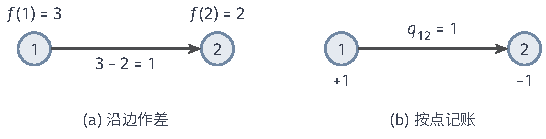
\includegraphics{figures/03-graphs/05-matrices-and-spectra/tikz/incidence-matrix-actions/figure.pdf}
  \caption{同一条参考边$1\to2$上的两种对偶运算。(a) 沿边差分算子$\bm{B}^\top$将两端顶点读数作差，得到边分量$d_{12}=f(1)-f(2)=1$。(b) 净流出汇总算子$\bm{B}$将该边上的单位正向流量$q_{12}=1$分配到两端，尾端净流出为$+1$，头端净流出为$-1$。}
  \label{fig:incidence-matrix-actions}
\end{BookInlineFigure}

\paragraph{伴随恒等式}

沿边差分算子$\bm{B}^\top\colon\mathbb{R}^V\to\mathbb{R}^E$与按顶点汇总算子$\bm{B}\colon\mathbb{R}^E\to\mathbb{R}^V$在矩阵形式上互为转置，在几何上则关于顶点内积与边内积互为伴随算子。

任取一个顶点函数$\bm{f}\in\mathbb{R}^V$和一个边流量向量$\bm{q}\in\mathbb{R}^E$。先算出沿边差分向量$\bm{B}^\top\bm{f}\in\mathbb{R}^E$，再与$\bm{q}$在边空间中作内积，按式~\eqref{eq:incidence-edge-inner-product}展开为对所有边的求和：
\[
\langle\bm{B}^\top\bm{f},\bm{q}\rangle_E
=\sum_{e\colon u\to v}\bigl(f(u)-f(v)\bigr)q_e
=\sum_{e\colon u\to v}\bigl(f(u)q_e-f(v)q_e\bigr).
\]
在最右端的求和式中，每条边$e\colon u\to v$产生了两项：尾端$u$处带有正号项$+f(u)q_e$，头端$v$处带有负号项$-f(v)q_e$。现在把求和次序从“逐边相加”改为“逐顶点归并”：固定一个顶点$w\in V$，把所有以$w$为尾端的边所贡献的$+f(w)q_e$与所有以$w$为头端的边所贡献的$-f(w)q_e$收集到一起，提出公因子$f(w)$，括号内剩下的恰好就是式~\eqref{eq:incidence-net-outflow}中顶点$w$的净流出量$(\bm{B}\bm{q})_w$：
\[
\begin{aligned}
\sum_{e\colon u\to v}\bigl(f(u)q_e-f(v)q_e\bigr)
&=\sum_{w\in V}f(w)\Biggl(\sum_{e:\,w\text{ 是尾端}}q_e-\sum_{e:\,w\text{ 是头端}}q_e\Biggr)\\
&=\sum_{w\in V}f(w)(\bm{B}\bm{q})_w.
\end{aligned}
\]
根据顶点内积定义式~\eqref{eq:incidence-vertex-inner-product}，最右端正是$\bm{f}$与净流出向量$\bm{B}\bm{q}$在顶点空间中的内积。于是我们得到伴随恒等式：
\begin{equation}
\langle\bm{B}^\top\bm{f},\bm{q}\rangle_E
=\langle\bm{f},\bm{B}\bm{q}\rangle_V.
\label{eq:incidence-adjoint-pairing}
\end{equation}
从代数上看，式~\eqref{eq:incidence-adjoint-pairing}就是向量内积的转置性质$(\bm{B}^\top\bm{f})^\top\bm{q}=\bm{f}^\top(\bm{B}\bm{q})$；从图上的记账来看，它表明“按每条边把两端读数差乘以边流量再求和”与“按每个顶点把读数乘以净流出量再求和”算的是同一笔总账。下一节证明环空间与割空间正交时，这一恒等式将起到核心作用。

最后说明参考方向的选择对计算结果的影响。如果将某一条边$e$的参考方向从$u\to v$反转为$v\to u$，矩阵$\bm{B}$的第$e$列随之变号；与此同时，同一股实际流量在新参考方向下的坐标$q_e$也变号。在计算$\bm{B}\bm{q}$时，列向量的负号与流量坐标的负号相乘抵消，因此每个顶点的净流出量$(\bm{B}\bm{q})_v$完全不变。

同理，沿边差分分量$(\bm{B}^\top\bm{f})_e$虽随参考方向变号，但与同样变号的$q_e$相乘后乘积不变。这意味着参考方向只是边空间坐标系的符号约定，顶点处的物理守恒关系以及下一节建立的子空间结构均不依赖于参考方向的具体选取。

\section{环空间与割空间}
\label{sec:graph-cycle-cut-spaces}

上一节建立了关联矩阵的两种对偶运算：沿边差分算子$\bm{B}^\top\colon\mathbb{R}^V\to\mathbb{R}^E$把顶点函数变成沿边差分向量，净流出汇总算子$\bm{B}\colon\mathbb{R}^E\to\mathbb{R}^V$把边流量向量变成各顶点的净流出量。这两个算子在边空间$\mathbb{R}^E$中自然划分出两类核心子空间——在所有顶点处净流出均为零的边流量构成环空间$\ker\bm{B}$，由顶点函数沿边差分生成的边向量构成割空间$\operatorname{im}\bm{B}^\top$。

本节依次建立这两个子空间的定义、正交直和分解与维数公式，最后利用生成森林构造出两组可直接读出坐标的显式基。

\subsection{环空间}
\label{sec:incidence-cycle-space}

我们先在图~\ref{fig:incidence-running-example}的四点五边图上考察什么样的边流量向量能使每个顶点的净流出量都等于零。

第一股流量沿外圈四元环$1\to2\to3\to4\to1$依次输送$1$个单位，对角边$13$上不送流。在每个顶点处核对进出账目：在顶点$1$，边$12$流出$1$个单位、边$41$流入$1$个单位，净流出为零；在顶点$2$，边$12$流入$1$个单位、边$23$流出$1$个单位，净流出也为零；顶点$3$与顶点$4$同理。因为外圈四条边的绕行方向与图~\ref{fig:incidence-running-example}约定的参考方向完全一致，按边序$(12,23,34,41,13)$记录，这股边流量向量为
\[
\bm{c}_1=(1,1,1,1,0)^\top.
\]
代入关联矩阵直接验算，确实有$\bm{B}\bm{c}_1=\bm{0}$。

第二股流量沿三角形回路$1\to3\to2\to1$绕行$1$个单位，外圈边$34$和$41$上不送流。逐边核对绕行方向与参考方向的关系：在对角边$13$上，绕行从$1$到$3$，与参考方向$1\to3$一致，分量取$+1$；在边$23$和边$12$上，绕行分别从$3$到$2$、从$2$到$1$，均与各自的参考方向（$2\to3$和$1\to2$）相反，分量均取$-1$；边$34$与$41$不在该三角形回路上，分量均取$0$。于是这股三角形环流写成边流量向量为
\[
\bm{c}_2=(-1,-1,0,0,1)^\top.
\]
逐行计算$\bm{B}\bm{c}_2$，每个顶点的流入与流出同样精确抵消，满足$\bm{B}\bm{c}_2=\bm{0}$。

由于矩阵乘法是线性的，两股处处守恒的边流量相加后依然满足守恒条件：$\bm{B}(\bm{c}_1+\bm{c}_2)=\bm{B}\bm{c}_1+\bm{B}\bm{c}_2=\bm{0}$。把两个向量逐分量相加：
\[
\bm{c}_1+\bm{c}_2=(1,1,1,1,0)^\top+(-1,-1,0,0,1)^\top=(0,0,1,1,1)^\top.
\]
图~\ref{fig:incidence-circulation-superposition}展示了这一叠加过程：在公共边$12$和$23$上，$\bm{c}_1$的正向单位流$+1$与$\bm{c}_2$的反向单位流$-1$恰好正反抵消、合成为零流量；剩下的三条边$34,41,13$首尾相接，恰好构成沿右下方三角形$1\to3\to4\to1$绕行的单位环流。同理，将任意守恒流量乘以实数倍，在每个顶点处的流入和流出按同一比例缩放，净流出量仍然为零。

\begin{BookInlineFigure}
  \centering
  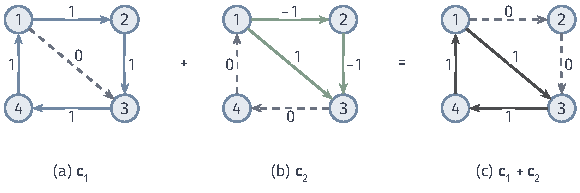
\includegraphics{figures/03-graphs/05-matrices-and-spectra/tikz/incidence-circulation-superposition/figure.pdf}
  \caption{四点五边图上两股环流的叠加$\bm{c}_1+\bm{c}_2$。边旁数字为对应参考方向下的流量分量，虚线表示流量为零。(a) 沿外圈$1\to2\to3\to4\to1$的单位环流$\bm{c}_1$。(b) 沿三角形$1\to3\to2\to1$的单位环流$\bm{c}_2$，其中边$12,23$因逆参考方向而取$-1$。(c) 叠加结果在边$12,23$上正反抵消为零，化为沿三角形$1\to3\to4\to1$的单位环流。}
  \label{fig:incidence-circulation-superposition}
\end{BookInlineFigure}

把“每个顶点处净流出量均为零”这一守恒条件写成一般形式，就得到环流与环空间的严格定义。

\begin{definition}[环流与环空间]
\label{def:graph-cycle-space}
设$\mathcal{G}=(V,E)$为有限图，$\bm{B}\in\mathbb{R}^{n\times m}$为其关联矩阵。若边流量向量$\bm{q}\in\mathbb{R}^E$在每个顶点处的净流出量均为零，即满足
\[
(\bm{B}\bm{q})_v=0\quad(\forall\,v\in V),
\qquad\text{或等价地}\qquad \bm{B}\bm{q}=\bm{0},
\]
则称$\bm{q}$为图$\mathcal{G}$上的一个\term{环流}（circulation）。全体实数环流构成的边空间线性子空间（即关联矩阵$\bm{B}\colon\mathbb{R}^E\to\mathbb{R}^V$的零空间）称为图$\mathcal{G}$的\term{环空间}（cycle space），记为
\begin{equation}
\mathcal{C}(\mathcal{G})=\{\bm{q}\in\mathbb{R}^E:\bm{B}\bm{q}=\bm{0}\}
=\ker\bm{B}.
\label{eq:incidence-cycle-space}
\end{equation}
\end{definition}

需要注意，本章定义的环空间$\mathcal{C}(\mathcal{G})$是实数域$\mathbb{R}$上的线性子空间：每条边可以承载任意实数大小的流量，负分量表示流向与参考方向相反。这与组合图论中在二元域$\mathbb{F}_2$（模$2$加法）下讨论的边子集对称差不同——在实数环空间中，两股同向的单位环流相加会变成$2$倍流量的环流，只有方向相反、大小相等的两股流量叠加才会抵消为零。

一般而言，环空间$\mathcal{C}(\mathcal{G})$中的元素既可以是沿单个简单环绕行的流量，也可以是由多个不同环路按任意实系数线性叠加而成的复合守恒流。那么，任意一个复杂的环流是否都能由少数几个基本简单环线性表出？第~\ref{sec:incidence-fundamental-bases}小节将利用生成森林给出肯定的回答与具体构造方法。在此之前，我们先考察边空间中由沿边差分生成的另一半子空间。

\subsection{割空间}
\label{sec:incidence-cut-space}

现在从相反的方向在边空间$\mathbb{R}^E$中生成向量：先给定顶点函数$\bm{f}\in\mathbb{R}^V$，再通过沿边差分算子$\bm{B}^\top$计算沿边差分向量$\bm{d}=\bm{B}^\top\bm{f}\in\mathbb{R}^E$。

最简单的一类顶点函数是将顶点集$V$分成两部分、在一侧赋$1$而在另一侧赋$0$的指示函数。任取顶点子集$S\subseteq V$，记其补集为$\bar{S}=V\setminus S$，令指示向量$\bm{1}_S\in\mathbb{R}^V$在$S$内的顶点上取$1$、在$\bar{S}$内的顶点上取$0$。对$\bm{1}_S$作用沿边差分算子，得到边空间中的列向量
\[
\bm{d}_S=\bm{B}^\top\bm{1}_S\in\mathbb{R}^E.
\]
对任意一条参考方向为$e\colon u\to v$的边，其分量$(\bm{d}_S)_e=\bm{1}_S(u)-\bm{1}_S(v)$只有三种可能取值：
\begin{itemize}
\item 若$u\in S$且$v\in\bar{S}$（边沿参考方向从$S$穿出到$\bar{S}$），则$(\bm{d}_S)_e=1-0=+1$；
\item 若$u\in\bar{S}$且$v\in S$（边沿参考方向从$\bar{S}$穿入到$S$），则$(\bm{d}_S)_e=0-1=-1$；
\item 若$u,v$同属于$S$或同属于$\bar{S}$（边不跨越割$(S,\bar{S})$），则$(\bm{d}_S)_e=0$。
\end{itemize}
因此，$\bm{d}_S$只在跨越割$(S,\bar{S})$的边上非零，称为对应于顶点子集$S$的\emph{割向量}（或带符号割指示向量）。

以四点五边图上的子集$S=\{1,2\}$及其补集$\bar{S}=\{3,4\}$为例。此时顶点指示向量为$\bm{1}_S=(1,1,0,0)^\top$。按边序$(12,23,34,41,13)$逐条检查五条边的端点位置：边$12$（$1\to2$）两端都在$S$内，差值为$1-1=0$；边$34$（$3\to4$）两端都在$\bar{S}$内，差值为$0-0=0$；边$23$（$2\to3$）和边$13$（$1\to3$）分别从$S$内的顶点$2,1$指向$\bar{S}$内的顶点$3$，差值均为$1-0=+1$；边$41$（$4\to1$）从$\bar{S}$内的$4$指向$S$内的$1$，差值为$0-1=-1$。汇总起来，子集$S=\{1,2\}$生成的割向量为
\[
\bm{d}_S=\bm{B}^\top\bm{1}_S=(0,1,0,-1,1)^\top\in\mathbb{R}^5.
\]
图~\ref{fig:incidence-cut-vector-example}直观展示了这一过程：左图以虚线将顶点集划分为上侧$S=\{1,2\}$（读数$1$）与下侧$\bar{S}=\{3,4\}$（读数$0$）；右图标出经$\bm{B}^\top$作用后各边上的差分分量，内部边$12,34$分量为$0$，三条跨割边$23,41,13$按穿行方向分别取$+1,-1,+1$。

\begin{BookInlineFigure}
  \centering
  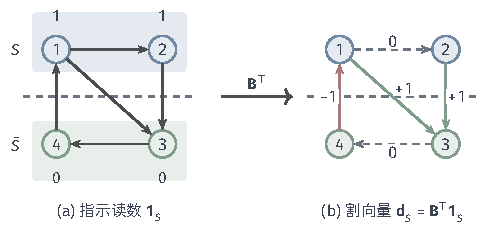
\includegraphics{figures/03-graphs/05-matrices-and-spectra/tikz/incidence-cut-vector-example/figure.pdf}
  \caption{四点五边图上子集$S=\{1,2\}$对应的割向量构造。(a) 将顶点划分为$S=\{1,2\}$（蓝底，赋读数$1$）与$\bar{S}=\{3,4\}$（绿底，赋读数$0$），构成顶点指示向量$\bm{1}_S=(1,1,0,0)^\top$。(b) 经沿边差分算子$\bm{B}^\top$作用后得到的割向量$\bm{d}_S=(0,1,0,-1,1)^\top$：同侧边$12,34$（虚线）差值为$0$，从$S$指向$\bar{S}$的跨割边$23,13$（绿线）取$+1$，从$\bar{S}$指向$S$的跨割边$41$（红线）取$-1$。}
  \label{fig:incidence-cut-vector-example}
\end{BookInlineFigure}

不仅$0$--$1$指示函数如此，任意一个实值顶点函数$\bm{f}\in\mathbb{R}^V$都可以按单点指示向量（即标准基向量$\bm{1}_{\{v\}}=\bm{e}_v$）展开为$\bm{f}=\sum_{v\in V}f(v)\bm{1}_{\{v\}}$。利用矩阵乘法的线性性，它的沿边差分向量可以写成
\[
\bm{B}^\top\bm{f}
=\sum_{v\in V}f(v)\,\bm{B}^\top\bm{1}_{\{v\}}
=\sum_{v\in V}f(v)\,\bm{d}_{\{v\}}.
\]
上式右端每一项都是单点割向量$\bm{d}_{\{v\}}=\bm{B}^\top\bm{1}_{\{v\}}$的数乘。这说明：任意顶点函数的沿边差分向量都是割向量的线性组合；反过来，任意一组割向量的线性组合$\sum_k\alpha_k\bm{B}^\top\bm{1}_{S_k}=\bm{B}^\top\bigl(\sum_k\alpha_k\bm{1}_{S_k}\bigr)$也必定是某个顶点函数的沿边差分向量。由此我们给出割空间的形式化定义。

\begin{definition}[割空间]
\label{def:graph-cut-space}
设$\mathcal{G}=(V,E)$为有限图，$\bm{B}\in\mathbb{R}^{n\times m}$为其关联矩阵。若边向量$\bm{d}\in\mathbb{R}^E$可以表示为某个顶点函数$\bm{f}\in\mathbb{R}^V$的沿边差分向量，即存在$\bm{f}\in\mathbb{R}^V$使得
\[
\bm{d}=\bm{B}^\top\bm{f}\qquad\bigl(\text{即对每条边 }e\colon u\to v\text{ 有 }d_e=f(u)-f(v)\bigr),
\]
则称$\bm{d}$为图$\mathcal{G}$上的一个沿边差分向量（或割差分向量）。全体顶点函数的沿边差分向量构成的边空间线性子空间（即沿边差分算子$\bm{B}^\top\colon\mathbb{R}^V\to\mathbb{R}^E$的像空间）称为图$\mathcal{G}$的\term{割空间}（cut space），记为
\begin{equation}
\mathcal{D}(\mathcal{G})=\{\bm{B}^\top\bm{f}:\bm{f}\in\mathbb{R}^V\}=\operatorname{im}\bm{B}^\top.
\label{eq:incidence-cut-space}
\end{equation}
\end{definition}

\paragraph{正交直和分解}

把定义~\ref{def:graph-cycle-space}与定义~\ref{def:graph-cut-space}放在一起，一个核心几何事实立刻浮现：环空间$\mathcal{C}(\mathcal{G})=\ker\bm{B}$与割空间$\mathcal{D}(\mathcal{G})=\operatorname{im}\bm{B}^\top$在边空间$\mathbb{R}^E$中正交互补。

先验证正交性。任取一个环流$\bm{c}\in\mathcal{C}(\mathcal{G})=\ker\bm{B}$和一个沿边差分向量$\bm{d}=\bm{B}^\top\bm{f}\in\mathcal{D}(\mathcal{G})$。根据式~\eqref{eq:incidence-adjoint-pairing}的伴随恒等式，二者在边空间中的内积为
\[
\langle\bm{d},\bm{c}\rangle_E
=\langle\bm{B}^\top\bm{f},\bm{c}\rangle_E
=\langle\bm{f},\bm{B}\bm{c}\rangle_V
=\langle\bm{f},\bm{0}\rangle_V=0,
\]
其中倒数第二步直接使用了环流的守恒条件$\bm{B}\bm{c}=\bm{0}$。

用简单环路可以直观看出两个向量内积为何恒为零。比如沿三角形$1\to2\to3\to1$绕行一圈的单位环流，将它与任意顶点函数$\bm{f}$的沿边差分作内积，相当于把沿环三步的端点差逐段相加：
\[
\bigl(f(1)-f(2)\bigr)+\bigl(f(2)-f(3)\bigr)+\bigl(f(3)-f(1)\bigr)=0.
\]
环上的每个顶点读数恰好出现两次——在离开该点的一步中取正号，在进入该点的一步中取负号——绕行闭合回路一圈后必然首尾相消（对应物理学中的基尔霍夫电压定律：保守势场沿任意闭合回路的电势降之和为零）。

不仅如此，割空间$\mathcal{D}(\mathcal{G})$的正交补$\mathcal{D}(\mathcal{G})^\perp$恰好就是整个环空间$\mathcal{C}(\mathcal{G})$。事实上，设边向量$\bm{q}\in\mathbb{R}^E$与割空间中的每一个沿边差分向量都正交，即对任意$\bm{f}\in\mathbb{R}^V$都有
\[
0=\langle\bm{B}^\top\bm{f},\bm{q}\rangle_E=\langle\bm{f},\bm{B}\bm{q}\rangle_V.
\]
由于上式对所有顶点函数$\bm{f}\in\mathbb{R}^V$均成立，特别地取$\bm{f}=\bm{B}\bm{q}\in\mathbb{R}^V$，即得
\[
\lVert\bm{B}\bm{q}\rVert_2^2=\langle\bm{B}\bm{q},\bm{B}\bm{q}\rangle_V=0,
\]
从而$\bm{B}\bm{q}=\bm{0}$，说明$\bm{q}\in\ker\bm{B}=\mathcal{C}(\mathcal{G})$。在有限维欧氏空间中，任意子空间与其正交补构成整个空间的正交直和（可参考\BookChapterRef{chap:inner-product-spaces}{卷二"内积空间"章}），因此边空间$\mathbb{R}^E$具有正交直和分解：
\begin{equation}
\mathbb{R}^E=\mathcal{C}(\mathcal{G})\oplus\mathcal{D}(\mathcal{G})
=\ker\bm{B}\oplus\operatorname{im}\bm{B}^\top.
\label{eq:incidence-edge-space-decomposition}
\end{equation}

式~\eqref{eq:incidence-edge-space-decomposition}表明，图上的任意边向量$\bm{q}\in\mathbb{R}^E$都可以唯一地分解为一个守恒环流$\bm{c}\in\mathcal{C}(\mathcal{G})$与一个沿边差分向量$\bm{d}\in\mathcal{D}(\mathcal{G})$之和：$\bm{q}=\bm{c}+\bm{d}$且$\langle\bm{c},\bm{d}\rangle_E=0$。分解的唯一性由正交性直接保证：若另有$\bm{q}=\bm{c}'+\bm{d}'$，相减得$\bm{c}-\bm{c}'=\bm{d}'-\bm{d}$；该差向量同时属于相互正交的$\mathcal{C}(\mathcal{G})$与$\mathcal{D}(\mathcal{G})$，故与自身的内积为零，只能是零向量。

我们用四点五边图上的边向量$\bm{q}=(1,2,1,0,1)^\top$验证这一正交分解：
\[
\bm{q}=\underbrace{(1,1,1,1,0)^\top}_{\bm{c}_1\in\mathcal{C}(\mathcal{G})}
      +\underbrace{(0,1,0,-1,1)^\top}_{\bm{d}_S\in\mathcal{D}(\mathcal{G})},
\]
其中第一项是外圈单位环流$\bm{c}_1$，第二项是子集$S=\{1,2\}$生成的割向量$\bm{d}_S$。容易核对$\langle\bm{c}_1,\bm{d}_S\rangle_E=0+1+0-1+0=0$。例如在边$41$上，环流分量$+1$与割差分分量$-1$叠加后恰好给出$q_{41}=0$；在边$23$上，两项同为$+1$，叠加给出$q_{23}=2$。图~\ref{fig:incidence-flow-decomposition}在三个并排面板中展示了$\bm{q}$、$\bm{c}_1$与$\bm{d}_S$的逐边分量关系。

\begin{BookInlineFigure}
  \centering
  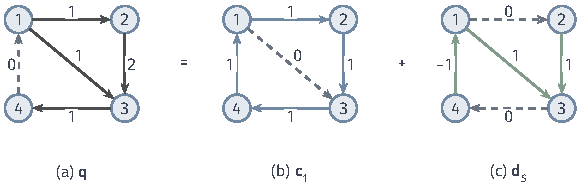
\includegraphics{figures/03-graphs/05-matrices-and-spectra/tikz/incidence-flow-decomposition/figure.pdf}
  \caption{四点五边图上的边向量正交分解$\bm{q}=\bm{c}_1+\bm{d}_S$，其中$S=\{1,2\}$。每条边旁的数值是对应参考方向下的边分量，虚线表示分量为零。}
  \label{fig:incidence-flow-decomposition}
\end{BookInlineFigure}

需要指出的是：虽然边向量$\bm{q}$分解出的沿边差分分量$\bm{d}\in\mathcal{D}(\mathcal{G})$是唯一的，但满足$\bm{B}^\top\bm{f}=\bm{d}$的原像顶点函数$\bm{f}\in\mathbb{R}^V$并不唯一——给$\bm{f}$加上任意属于零空间$\ker\bm{B}^\top$的向量，沿边差分向量$\bm{B}^\top\bm{f}$都保持不变。下一小节通过刻画$\ker\bm{B}^\top$的具体结构，精确算出关联矩阵的秩以及环空间、割空间的维数。

\subsection{子空间维数}
\label{sec:incidence-rank-dimensions}

要计算割空间$\mathcal{D}(\mathcal{G})=\operatorname{im}\bm{B}^\top$与环空间$\mathcal{C}(\mathcal{G})=\ker\bm{B}$各自的维数，关键在于先搞清楚：什么样的顶点函数$\bm{f}\in\mathbb{R}^V$在经过沿边差分算子$\bm{B}^\top$作用后会变成零向量？也就是说，零空间$\ker\bm{B}^\top=\{\bm{f}\in\mathbb{R}^V:\bm{B}^\top\bm{f}=\bm{0}\}$具有什么结构、维数是多少？下面我们分四步把推理过程完整展开。

\paragraph{第一步：同一连通分量内的顶点读数必定相等}

根据沿边差分的定义式~\eqref{eq:incidence-edge-difference}，$\bm{B}^\top\bm{f}=\bm{0}$等价于在每一条边$e\colon u\to v\in E$上都有
\[
f(u)-f(v)=0,\qquad\text{即}\qquad f(u)=f(v).
\]
这表明，只要两个顶点之间有一条边直接相连，它们的读数就必须相等。更进一步，如果两个顶点$i$和$j$属于图的同一个连通分量，那么按连通性的定义，图中存在一条连接$i$与$j$的路径$i=w_0,w_1,\ldots,w_s=j$，其中相邻两步$\{w_{r-1},w_r\}$都是图中的边。沿这条路径逐边应用“相邻端点读数相等”，便得到传递链：
\[
f(i)=f(w_0)=f(w_1)=\cdots=f(w_s)=f(j).
\]
因此，任何满足$\bm{B}^\top\bm{f}=\bm{0}$的顶点函数$\bm{f}$，在图的每一个连通分量内部都必须取同一个常数值。

\paragraph{第二步：不同连通分量之间的常数可以彼此独立选取}

如果整张图$\mathcal{G}$是连通的（只有$1$个连通分量），那么上面第一步已经说明所有$n$个顶点的读数都必须等于同一个常数$\alpha_1$。但如果图$\mathcal{G}$不连通，设它的顶点集$V$划分为$c$个互不相交的连通分量（connected components）：
\[
V=V_1\cup V_2\cup\cdots\cup V_c.
\]
为什么每个连通分量$V_k$可以各自独立地任选一个常数$\alpha_k\in\mathbb{R}$，而不会违反$\bm{B}^\top\bm{f}=\bm{0}$？

原因在于：不同连通分量$V_k$与$V_\ell$（$k\neq\ell$）之间没有任何边相连。换言之，图$\mathcal{G}$中的每一条边$e\colon u\to v\in E$，其两个端点$u$和$v$必定同时落在某一个连通分量$V_k$内部，绝不会出现一端在$V_k$、另一端在$V_\ell$的跨分量边。于是，只要我们在第$1$个连通分量$V_1$的所有顶点上统一赋常数$\alpha_1$，在第$2$个连通分量$V_2$的所有顶点上统一赋常数$\alpha_2$，……，在第$c$个连通分量$V_c$的所有顶点上统一赋常数$\alpha_c$，那么对任意一条边$e\colon u\to v$（不妨设它落在$V_k$内），两端的读数差就恒为
\[
f(u)-f(v)=\alpha_k-\alpha_k=0.
\]
至于其他分量$V_\ell$（$\ell\neq k$）上选了什么常数$\alpha_\ell$，没有边把$\alpha_\ell$和$\alpha_k$连起来作差，因此$\alpha_1,\alpha_2,\ldots,\alpha_c$这$c$个实数彼此之间没有任何耦合约束，可以完全独立地任意取值。特别地，若图中某个顶点$v$是不连任何边的孤立顶点（isolated vertex），它自己单独构成一个连通分量$V_k=\{v\}$；由于没有任何边以$v$为端点，$f(v)=\alpha_k$不出现在$\bm{B}^\top\bm{f}$的任何分量中，也可以独立任取一个实数。

\paragraph{第三步：用分量指示向量表示零空间$\ker\bm{B}^\top$}

为了把“在每个连通分量$V_k$上各自独立取常数$\alpha_k$”写成标准的线性代数语言，我们对第$k$个连通分量$V_k$（$k=1,\ldots,c$）定义其\emph{分量指示向量}$\bm{1}_{V_k}\in\mathbb{R}^V$：
\[
(\bm{1}_{V_k})_v=
\begin{cases}
1,& v\in V_k,\\
0,& v\notin V_k.
\end{cases}
\]
这样，给第$k$个分量的所有顶点赋常数$\alpha_k$，合在一起写成列向量就是线性组合
\begin{equation}
\bm{f}=\alpha_1\bm{1}_{V_1}+\alpha_2\bm{1}_{V_2}+\cdots+\alpha_c\bm{1}_{V_c}.
\label{eq:incidence-ker-bt-expansion}
\end{equation}
我们来逐坐标核对式~\eqref{eq:incidence-ker-bt-expansion}：任取图中的一个顶点$v\in V$，因为$V=V_1\cup\cdots\cup V_c$是互不相交的划分，$v$恰好属于唯一的一个连通分量$V_k$。在顶点$v$所在的坐标位置上，只有$\bm{1}_{V_k}$取$1$，其余$c-1$个指示向量$\bm{1}_{V_\ell}$（$\ell\neq k$）全部取$0$，因此式~\eqref{eq:incidence-ker-bt-expansion}右端在顶点$v$处的值恰好是
\[
\alpha_1\cdot 0+\cdots+\alpha_k\cdot 1+\cdots+\alpha_c\cdot 0=\alpha_k=f(v).
\]
这证明了：$\bm{f}\in\ker\bm{B}^\top$当且仅当$\bm{f}$可以写成式~\eqref{eq:incidence-ker-bt-expansion}的形式。也就是说，这$c$个分量指示向量$\{\bm{1}_{V_1},\ldots,\bm{1}_{V_c}\}$张成了整个零空间$\ker\bm{B}^\top$。

\paragraph{第四步：证明$c$个分量指示向量线性无关}

要确认$\{\bm{1}_{V_1},\ldots,\bm{1}_{V_c}\}$构成$\ker\bm{B}^\top$的一组基，还需证明它们线性无关。设有一组实系数$\alpha_1,\ldots,\alpha_c\in\mathbb{R}$使线性组合等于零向量：
\[
\alpha_1\bm{1}_{V_1}+\alpha_2\bm{1}_{V_2}+\cdots+\alpha_c\bm{1}_{V_c}=\bm{0}.
\]
对任意下标$k\in\{1,\ldots,c\}$，连通分量$V_k$都是非空顶点子集，我们在$V_k$中任取一个代表顶点$v\in V_k$，读取上式左右两端在第$v$个坐标处的分量：左端等于$\alpha_k$，右端等于零向量的分量$0$，故必有$\alpha_k=0$。由于$k$是任意的，全部系数$\alpha_1=\alpha_2=\cdots=\alpha_c=0$。这证明了$\{\bm{1}_{V_1},\ldots,\bm{1}_{V_c}\}$线性无关，从而构成$\ker\bm{B}^\top$的一组基，零空间的维数恰等于连通分量个数$c$：
\[
\dim\ker\bm{B}^\top=c.
\]

我们用一个具体例子配合图~\ref{fig:incidence-component-constants}来直观核对上述推理。考虑由$n=5$个顶点、$c=2$个连通分量组成的图：第一个分量$V_1=\{1,2,3\}$是一个三角形，第二个分量$V_2=\{4,5\}$是一条独立边。两个分量的指示向量分别为
\[
\bm{1}_{V_1}=(1,1,1,0,0)^\top,\qquad
\bm{1}_{V_2}=(0,0,0,1,1)^\top.
\]
它们的任意线性组合为
\[
\bm{f}=\alpha_1\bm{1}_{V_1}+\alpha_2\bm{1}_{V_2}
=(\alpha_1,\alpha_1,\alpha_1,\alpha_2,\alpha_2)^\top.
\]
如图~\ref{fig:incidence-component-constants}(c)所示，三角形内部三条边的两端读数均为$\alpha_1$，差值为$\alpha_1-\alpha_1=0$；底边$\{4,5\}$的两端读数均为$\alpha_2$，差值为$\alpha_2-\alpha_2=0$；而$V_1$与$V_2$之间没有边相连，$\alpha_1$与$\alpha_2$永远不会被放在同一条边上相减。若令$\bm{f}=(0,0,0,0,0)^\top$，从顶点$1$读出$\alpha_1=0$，从顶点$4$读出$\alpha_2=0$，两个指示向量显然线性无关，张成二维零空间$\ker\bm{B}^\top$。

\begin{BookInlineFigure}
  \centering
  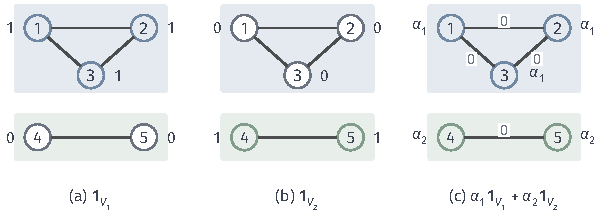
\includegraphics{figures/03-graphs/05-matrices-and-spectra/tikz/incidence-component-constants/figure.pdf}
  \caption{含$c=2$个连通分量$V_1=\{1,2,3\}$（蓝底）与$V_2=\{4,5\}$（绿底）的五点图上$\ker\bm{B}^\top$的基与通解。(a) 第一分量指示向量$\bm{1}_{V_1}=(1,1,1,0,0)^\top$。(b) 第二分量指示向量$\bm{1}_{V_2}=(0,0,0,1,1)^\top$。(c) 一般零空间向量$\bm{f}=\alpha_1\bm{1}_{V_1}+\alpha_2\bm{1}_{V_2}$在两个分量上分别取独立常数$\alpha_1,\alpha_2$，每条边的两端同属一个分量，沿边差分全为$0$。}
  \label{fig:incidence-component-constants}
\end{BookInlineFigure}

有了$\dim\ker\bm{B}^\top=c$，连续使用两次线性代数的秩零度定理（rank-nullity theorem），即可直接导出关联矩阵的秩以及割空间、环空间的维数公式。

\begin{theorem}[环空间与割空间的维数]
\label{thm:incidence-cycle-cut-dimensions}
设有限图$\mathcal{G}=(V,E)$有$n$个顶点、$m$条边和$c$个连通分量，关联矩阵为$\bm{B}\in\mathbb{R}^{n\times m}$。则关联矩阵的秩为
\begin{equation}
\operatorname{rank}\bm{B}=\operatorname{rank}\bm{B}^\top=n-c,
\label{eq:incidence-rank-components}
\end{equation}
且割空间$\mathcal{D}(\mathcal{G})=\operatorname{im}\bm{B}^\top$与环空间$\mathcal{C}(\mathcal{G})=\ker\bm{B}$的维数分别为
\begin{equation}
\dim\mathcal{D}(\mathcal{G})=n-c,\qquad
\dim\mathcal{C}(\mathcal{G})=m-n+c.
\label{eq:incidence-cycle-cut-dimensions}
\end{equation}
\end{theorem}

\begin{proof}
首先考察沿边差分算子$\bm{B}^\top\colon\mathbb{R}^V\to\mathbb{R}^E$。它的定义域是$n$维顶点空间$\mathbb{R}^V$，零空间$\ker\bm{B}^\top$由$c$个连通分量的指示向量$\{\bm{1}_{V_1},\ldots,\bm{1}_{V_c}\}$张成且线性无关，故$\dim\ker\bm{B}^\top=c$。对线性映射$\bm{B}^\top$应用秩零度定理，其像空间$\mathcal{D}(\mathcal{G})=\operatorname{im}\bm{B}^\top$的维数为
\[
\dim\mathcal{D}(\mathcal{G})=\operatorname{rank}\bm{B}^\top=\dim\mathbb{R}^V-\dim\ker\bm{B}^\top=n-c.
\]
由于矩阵与其转置的秩相等，有$\operatorname{rank}\bm{B}=\operatorname{rank}\bm{B}^\top=n-c$，式~\eqref{eq:incidence-rank-components}得证。

再考察净流出汇总算子$\bm{B}\colon\mathbb{R}^E\to\mathbb{R}^V$。它的定义域是$m$维边空间$\mathbb{R}^E$，秩为$\operatorname{rank}\bm{B}=n-c$。对$\bm{B}$应用秩零度定理，其零空间$\mathcal{C}(\mathcal{G})=\ker\bm{B}$的维数为
\[
\dim\mathcal{C}(\mathcal{G})=\dim\ker\bm{B}=\dim\mathbb{R}^E-\operatorname{rank}\bm{B}=m-(n-c)=m-n+c.
\]
式~\eqref{eq:incidence-cycle-cut-dimensions}得证。
\end{proof}

验证两个具体情形：在图~\ref{fig:incidence-running-example}的四点五边图上，$n=4,m=5,c=1$，由定理~\ref{thm:incidence-cycle-cut-dimensions}立得割空间维数为$4-1=3$，环空间维数为$5-4+1=2$，两者之和$3+2=5=m$，与正交直和分解式~\eqref{eq:incidence-edge-space-decomposition}完全吻合。

又若图$\mathcal{G}$是一片不含任何环的森林（forest），则边数恰为$m=n-c$，此时环空间维数$\dim\mathcal{C}(\mathcal{G})=(n-c)-n+c=0$，即森林上不存在任何非零环流。直观上，无环图中任何非零流量一旦沿某条边流出，最终必然到达度为$1$的叶子顶点而无法绕回，从而在叶子处破坏流量守恒。下一小节将利用生成森林把这一观察转化为显式基的构造与证明。

\subsection{基本环基}
\label{sec:incidence-fundamental-bases}

定理~\ref{thm:incidence-cycle-cut-dimensions}给出了环空间维数$m-n+c$和割空间维数$n-c$，但还没有具体指明怎样找出一组基向量。注意到在一张有$n$个顶点、$c$个连通分量的图$\mathcal{G}=(V,E)$中，任取一棵生成森林$F\subseteq E$（当图连通、$c=1$时就是一棵生成树$T$），森林$F$中包含的\emph{树边}（tree edges）条数恰好是$n-c$，等于割空间的维数；而留在森林之外的\emph{非树边}（non-tree edges，也称弦，$E\setminus F$）条数恰好是$m-(n-c)=m-n+c$，等于环空间的维数。

这并非巧合：用每条非树边与树路径闭合，可以逐一构造出$m-n+c$个线性无关的基本环向量；下一小节再逐一删去每条树边将生成树切成两半，构造出$n-c$个线性无关的基本割向量。

下面说明如何由生成森林$F$和每一条非树边$e\in E\setminus F$构造基本环向量。取定一条非树边$e\colon u\to v\in E\setminus F$，由于$e$的两个端点$u$和$v$属于同一个连通分量，在生成森林$F$内部已经存在唯一一条连接$v$到$u$的树路径$P_e\subseteq F$；将非树边$e$添入$F$中，边集$P_e\cup\{e\}$就构成唯一一个简单环，记为$C_e$。规定沿环$C_e$的绕行方向与非树边$e$本身的参考方向$u\to v$一致（即先沿$e$从$u$走到$v$，再沿树路径$P_e$从$v$走回$u$），据此定义一个边流量向量$\bm{c}^{(e)}\in\mathbb{R}^E$：
\[
\bigl(\bm{c}^{(e)}\bigr)_{e'}=
\begin{cases}
+1,& e'=e\text{（即该非树边本身）},\\[2pt]
+1,& e'\in P_e\text{ 且 }e'\text{ 的参考方向与 }C_e\text{ 的绕行方向一致},\\[2pt]
-1,& e'\in P_e\text{ 且 }e'\text{ 的参考方向与 }C_e\text{ 的绕行方向相反},\\[2pt]
0,& e'\notin C_e\text{（包括其余所有非树边及不在 }P_e\text{ 上的树边）}.
\end{cases}
\]
向量$\bm{c}^{(e)}$称为对应于非树边$e$的\term{基本环}向量（fundamental cycle vector）。

我们在图~\ref{fig:incidence-running-example}的四点五边图上演示这一构造过程。如图~\ref{fig:incidence-fundamental-cycles}(a)所示，选取路径生成树$T=\{12,23,34\}$（共$n-1=3$条树边），留下的两条非树边为$E\setminus T=\{41,13\}$（共$m-n+1=2$条非树边）。

先添入非树边$41$（参考方向$4\to1$）：如图~\ref{fig:incidence-fundamental-cycles}(b)所示，沿非树边$41$从$4$走到$1$，再沿树路径$1\to2\to3\to4$返回$4$。沿途经过的三条树边$12,23,34$均与各自的参考方向同向（各取$+1$），另一条非树边$13$不在环上（取$0$），按边序$(12,23,34,41,13)$得到第一个基本环向量
\[
\bm{c}_1=\bm{c}^{(41)}=(1,1,1,\;1,0)^\top.
\]
再添入非树边$13$（参考方向$1\to3$）：如图~\ref{fig:incidence-fundamental-cycles}(c)所示，沿非树边$13$从$1$走到$3$，再沿树路径$3\to2\to1$返回$1$。返回途中经过的树边$23$和$12$均与各自的参考方向（$2\to3$和$1\to2$）相反，分量均取$-1$；树边$34$和另一条非树边$41$不在环上，均取$0$，得到第二个基本环向量
\[
\bm{c}_2=\bm{c}^{(13)}=(-1,-1,0,\;0,1)^\top.
\]

\begin{BookInlineFigure}
  \centering
  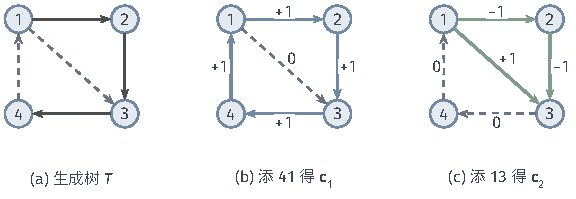
\includegraphics{figures/03-graphs/05-matrices-and-spectra/tikz/incidence-fundamental-cycles/figure.pdf}
  \caption{在四点五边图上由路径生成树$T=\{12,23,34\}$构造基本环基。(a) 实线为三条树边$12,23,34$，虚线为两条非树边$41,13$。(b) 添入非树边$41$并沿树路径$1\to2\to3\to4$闭合，得到基本环向量$\bm{c}_1=(1,1,1,1,0)^\top$。(c) 添入非树边$13$并沿树路径$3\to2\to1$闭合（逆参考方向经过$23$与$12$），得到基本环向量$\bm{c}_2=(-1,-1,0,0,1)^\top$。}
  \label{fig:incidence-fundamental-cycles}
\end{BookInlineFigure}

观察$\bm{c}_1$和$\bm{c}_2$在最后两个坐标——即两条非树边$(41,13)$——上的取值：$\bm{c}_1$在$(41,13)$处为$(1,0)^\top$，$\bm{c}_2$在$(41,13)$处为$(0,1)^\top$，拼在一起恰好是$2\times 2$单位矩阵$\bigl(\begin{smallmatrix}1&0\\0&1\end{smallmatrix}\bigr)$。每条非树边只出现在它自己生成的那个基本环中，而在其他所有基本环中坐标全为$0$。正是这一“非树边坐标呈单位阵”的结构，使基本环向量的线性无关性与坐标展开变得可以直接验证。

\begin{theorem}[基本环基]
\label{thm:incidence-fundamental-cycle-basis}
设有限图$\mathcal{G}=(V,E)$有$n$个顶点、$m$条边和$c$个连通分量，$F\subseteq E$为其一棵生成森林。则由$m-n+c$条非树边$e\in E\setminus F$构造的基本环向量集合
\[
\bigl\{\bm{c}^{(e)}:e\in E\setminus F\bigr\}
\]
构成环空间$\mathcal{C}(\mathcal{G})=\ker\bm{B}$的一组基。特别地，任意环流$\bm{q}\in\mathcal{C}(\mathcal{G})$均可按其在非树边上的分量唯一展开为
\begin{equation}
\bm{q}=\sum_{e\in E\setminus F}q_e\,\bm{c}^{(e)}.
\label{eq:incidence-fundamental-cycle-expansion}
\end{equation}
\end{theorem}

\begin{proof}
我们分三步证明：（1）每个$\bm{c}^{(e)}$属于$\mathcal{C}(\mathcal{G})$；（2）这$m-n+c$个向量线性无关；（3）任意环流$\bm{q}\in\mathcal{C}(\mathcal{G})$均满足展开式~\eqref{eq:incidence-fundamental-cycle-expansion}。

\textbf{第一步（属于环空间）}：对每条非树边$e\in E\setminus F$，$C_e$是一个简单闭合回路。不在$C_e$上的顶点关联的边流量全为$0$，净流出量为$0$；在$C_e$上的每个顶点恰好作为$C_e$中一条边的流入端和另一条边的流出端，按绕行方向一进一出各$1$个单位，根据关联矩阵作用公式~\eqref{eq:incidence-net-outflow}，其净流出量也为$1-1=0$。因此$\bm{B}\bm{c}^{(e)}=\bm{0}$，即$\bm{c}^{(e)}\in\mathcal{C}(\mathcal{G})$。

\textbf{第二步（线性无关）}：设有一组实系数$\{\alpha_e:e\in E\setminus F\}$使得
\[
\sum_{e'\in E\setminus F}\alpha_{e'}\,\bm{c}^{(e')}=\bm{0}.
\]
任取一条非树边$e\in E\setminus F$，读取上式两端在第$e$条边上的坐标分量。由基本环向量的构造规则，$\bm{c}^{(e)}$在边$e$上的分量为$1$，而其余所有基本环向量$\bm{c}^{(e')}$（$e'\neq e$）在非树边$e$上的分量全为$0$。因此上式左端在第$e$条边上的分量就是$\alpha_e\cdot 1+0=\alpha_e$，右端为$0$，故$\alpha_e=0$。对每条非树边$e\in E\setminus F$均如此，说明$\{\bm{c}^{(e)}:e\in E\setminus F\}$线性无关。

\textbf{第三步（张成性与唯一展开式）}：由定理~\ref{thm:incidence-cycle-cut-dimensions}，环空间的维数为$\dim\mathcal{C}(\mathcal{G})=m-n+c$，因此$\mathcal{C}(\mathcal{G})$中$m-n+c$个线性无关的向量已经构成一组基。为了直接导出展开式~\eqref{eq:incidence-fundamental-cycle-expansion}，任取环流$\bm{q}\in\ker\bm{B}$，直接用$\bm{q}$在各条非树边上的分量$q_e$作系数，构造余量向量
\[
\bm{r}=\bm{q}-\sum_{e\in E\setminus F}q_e\,\bm{c}^{(e)}.
\]
一方面，$\bm{r}$是环流的线性组合，故仍满足守恒条件$\bm{B}\bm{r}=\bm{0}$；另一方面，在每一条非树边$e\in E\setminus F$上，$r_e=q_e-q_e\cdot 1=0$。这意味着守恒流$\bm{r}$在所有非树边上全为零，只可能在生成森林$F$的树边上非零。

若$\bm{r}\neq\bm{0}$，设$F'\subseteq F$为$r_{e'}\neq 0$的树边子集。因为$F'$是森林的非空子图（无环），$F'$中必然存在一个只与$F'$中唯一一条边$e_1\in F'$相连的叶子顶点$v$。但在顶点$v$处，$\bm{r}$在关联于$v$的其余所有边上分量皆为$0$，故净流出量为$(\bm{B}\bm{r})_v=\pm r_{e_1}$；由守恒条件$(\bm{B}\bm{r})_v=0$立得$r_{e_1}=0$，与$e_1\in F'$矛盾。（等价地，从生成森林$F$的叶子顶点开始逐次剥去叶子与所连树边，每一步叶子处的守恒方程都迫使该树边流量为零，直至整片森林清空。）因此必有$\bm{r}=\bm{0}$，式~\eqref{eq:incidence-fundamental-cycle-expansion}得证。
\end{proof}

\subsection{基本割基}
\label{sec:incidence-fundamental-cut-bases}

与非树边生成基本环对偶，生成森林$F$中的每一条树边$e\in F$都可以用来构造一个基本割向量。取定一条树边$e\colon u\to v\in F$，设它属于连通分量$V_k$的生成树$T_k$。因为树是连通无环图，从$T_k$中删去树边$e$后，$T_k$恰好分裂成两棵互不连通的子树；取包含边$e$尾端$u$的那棵子树的顶点集为$S_e$（头端$v$落在另一侧$V\setminus S_e$中），以子集$S_e$的指示向量$\bm{1}_{S_e}\in\mathbb{R}^V$作用沿边差分算子$\bm{B}^\top$，定义
\[
\bm{d}^{(e)}=\bm{B}^\top\bm{1}_{S_e}\in\mathbb{R}^E.
\]
考察$\bm{d}^{(e)}$在各条边上的分量：在被删的树边$e\colon u\to v$本身上，尾端$u\in S_e$（读数$1$）、头端$v\notin S_e$（读数$0$），故$\bigl(\bm{d}^{(e)}\bigr)_e=1-0=+1$；在生成森林的其余所有树边$e'\in F\setminus\{e\}$上，删去$e$并没有切断$e'$，因此$e'$的两个端点必定同在$S_e$内或同在$S_e$外，两端读数相等，故$\bigl(\bm{d}^{(e)}\bigr)_{e'}=0$；在原图的非树边$e''\in E\setminus F$上，若$e''$跨越$S_e$与$V\setminus S_e$，则按参考方向从$S_e$穿出取$+1$、穿入取$-1$，不跨割则取$0$。向量$\bm{d}^{(e)}$称为对应于树边$e\in F$的\term{基本割}向量（fundamental cut vector）。

仍在四点五边图的路径生成树$T=\{12,23,34\}$上逐一构造全部$n-1=3$个基本割向量（边序仍为$12,23,34,41,13$），如图~\ref{fig:incidence-tree-cycle-cut}所示。

删去树边$12$（$1\to2$）时（图~\ref{fig:incidence-tree-cycle-cut}(a)），树$T$分裂为尾端侧$S_1=\{1\}$与头端侧$\bar{S}_1=\{2,3,4\}$，树边$12$从$S_1$指向$\bar{S}_1$（取$+1$），其余两条树边$23,34$两端都在$\bar{S}_1$内（取$0$），非树边$41$从$4$指向$1$（取$-1$），非树边$13$从$1$指向$3$（取$+1$），得到第一个基本割向量$\bm{d}_1=\bm{d}^{(12)}$。

删去树边$23$（$2\to3$）时（图~\ref{fig:incidence-tree-cycle-cut}(b)），树$T$分裂为$S_2=\{1,2\}$与$\bar{S}_2=\{3,4\}$，树边$23$取$+1$、树边$12,34$取$0$，非树边$41$取$-1$、$13$取$+1$，得到第二个基本割向量$\bm{d}_2=\bm{d}^{(23)}$。

删去树边$34$（$3\to4$）时（图~\ref{fig:incidence-tree-cycle-cut}(c)），树$T$分裂为$S_3=\{1,2,3\}$与$\bar{S}_3=\{4\}$，树边$34$取$+1$、树边$12,23$取$0$，非树边$41$从$4$进入$1$（取$-1$），非树边$13$两端都在$S_3$内（取$0$），得到第三个基本割向量$\bm{d}_3=\bm{d}^{(34)}$。三个基本割向量依次为
\[
\bm{d}_1=(1,0,0,\;-1,1)^\top,\quad
\bm{d}_2=(0,1,0,\;-1,1)^\top,\quad
\bm{d}_3=(0,0,1,\;-1,0)^\top.
\]

\begin{BookInlineFigure}
  \centering
  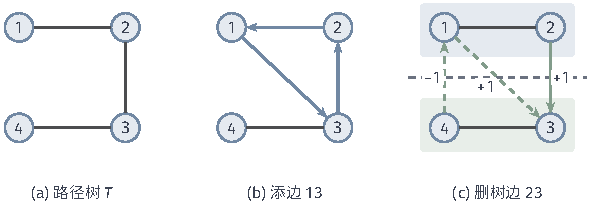
\includegraphics{figures/03-graphs/05-matrices-and-spectra/tikz/incidence-tree-cycle-cut/figure.pdf}
  \caption{在四点五边图上由路径生成树$T=\{12,23,34\}$构造三个基本割基向量。每个面板删去一条树边，蓝底标出含该树边尾端的子树顶点集$S_k$，绿底标出另一侧$\bar{S}_k$；绿实线（$+1$）和红实线（$-1$）为跨割边，灰虚线（$0$）为同侧边。(a) 删树边$12$，$S_1=\{1\}$，得$\bm{d}_1=(1,0,0,-1,1)^\top$。(b) 删树边$23$，$S_2=\{1,2\}$，得$\bm{d}_2=(0,1,0,-1,1)^\top$。(c) 删树边$34$，$S_3=\{1,2,3\}$，得$\bm{d}_3=(0,0,1,-1,0)^\top$。}
  \label{fig:incidence-tree-cycle-cut}
\end{BookInlineFigure}

观察$\bm{d}_1,\bm{d}_2,\bm{d}_3$在前三个坐标——即三条树边$(12,23,34)$——上的取值：它们依次为$(1,0,0)^\top,(0,1,0)^\top,(0,0,1)^\top$，拼在一起恰好是$3\times 3$单位矩阵。每条树边只出现在删去它自己时生成的那个基本割中，而在其余基本割中分量全为$0$。据此可立即证明基本割基定理。

\begin{theorem}[基本割基]
\label{thm:incidence-fundamental-cut-basis}
设有限图$\mathcal{G}=(V,E)$有$n$个顶点、$m$条边和$c$个连通分量，$F\subseteq E$为其一棵生成森林。则由$n-c$条树边$e\in F$构造的基本割向量集合
\[
\bigl\{\bm{d}^{(e)}:e\in F\bigr\}
\]
构成割空间$\mathcal{D}(\mathcal{G})=\operatorname{im}\bm{B}^\top$的一组基。特别地，任意割差分向量$\bm{d}\in\mathcal{D}(\mathcal{G})$均可按其在树边上的分量唯一展开为
\begin{equation}
\bm{d}=\sum_{e\in F}d_e\,\bm{d}^{(e)}.
\label{eq:incidence-fundamental-cut-expansion}
\end{equation}
\end{theorem}

\begin{proof}
首先，每个$\bm{d}^{(e)}=\bm{B}^\top\bm{1}_{S_e}$由顶点函数$\bm{1}_{S_e}$经$\bm{B}^\top$作用生成，故属于$\mathcal{D}(\mathcal{G})=\operatorname{im}\bm{B}^\top$。

其次证明线性无关。设有一组实系数$\{\beta_e:e\in F\}$使得
\[
\sum_{e'\in F}\beta_{e'}\,\bm{d}^{(e')}=\bm{0}.
\]
任取一条树边$e\in F$，读取上式两端在第$e$条边上的坐标分量。由基本割向量的构造规则，$\bm{d}^{(e)}$在树边$e$上的分量为$1$，而其余所有基本割向量$\bm{d}^{(e')}$（$e'\in F\setminus\{e\}$）在树边$e$上的分量全为$0$。因此左端在树边$e$处的分量就是$\beta_e\cdot 1+0=\beta_e$，右端为$0$，故$\beta_e=0$。这证明了$n-c$个基本割向量线性无关。

最后，由定理~\ref{thm:incidence-cycle-cut-dimensions}知割空间的维数为$\dim\mathcal{D}(\mathcal{G})=n-c$。在$n-c$维空间中，$n-c$个线性无关的向量$\{\bm{d}^{(e)}:e\in F\}$必然构成一组基。因此，任意$\bm{d}\in\mathcal{D}(\mathcal{G})$都可唯一展开为$\bm{d}=\sum_{e'\in F}\beta_{e'}\bm{d}^{(e')}$；读取两端在每条树边$e\in F$上的坐标分量，立得$d_e=\beta_e$，即展开式~\eqref{eq:incidence-fundamental-cut-expansion}成立。
\end{proof}

\paragraph{正交性的验证}

我们可以用四点五边图上求出的基本环基$\{\bm{c}_1,\bm{c}_2\}$与基本割基$\{\bm{d}_1,\bm{d}_2,\bm{d}_3\}$直接核对环空间与割空间的正交性。例如，取基本割向量$\bm{d}_2=(0,1,0,-1,1)^\top$，将其分别与$\bm{c}_1$和$\bm{c}_2$作内积：
\[
\begin{aligned}
\bm{c}_1^\top\bm{d}_2&=1\cdot0+1\cdot1+1\cdot0+1\cdot(-1)+0\cdot1=1-1=0,\\
\bm{c}_2^\top\bm{d}_2&=(-1)\cdot0+(-1)\cdot1+0\cdot0+0\cdot(-1)+1\cdot1=-1+1=0.
\end{aligned}
\]
从图上看，任何一个基本环一旦跨过基本割从$S_e$进入$\bar{S}_e$（贡献一次树边或非树边同向乘积），为了回到起点就必须再次跨过该割从$\bar{S}_e$返回$S_e$（贡献一次反向乘积），两次跨割的乘积符号相反、恰好成对抵消。

最后指出，换选另一棵生成树（或生成森林）会得到另一套基本环基和基本割基，基向量的具体坐标随之改变；但它们所张成的环空间$\mathcal{C}(\mathcal{G})=\ker\bm{B}$和割空间$\mathcal{D}(\mathcal{G})=\operatorname{im}\bm{B}^\top$本身只由原图的关联矩阵$\bm{B}$唯一确定，不随生成树的选择而改变。

\section{全幺模性}
\label{sec:graph-incidence-total-unimodularity}
\label{sec:incidence-tu-definition}

前面两节建立了顶点函数和边函数的空间，并给出了正交分解和维数。现在转向另一个问题：如果把图上的流量或选边写成线性规划，什么时候即使放开整数约束，最优解仍然是整数？答案取决于系数矩阵的方子式——这就是全幺模性。

举一个小例子。矩阵
\[
\bm{M}=\begin{pmatrix}1&1\\1&-1\end{pmatrix}
\]
的每个条目都是$\pm1$，但$\det\bm{M}=1\cdot(-1)-1\cdot1=-2$。以$(1,0)^\top$为右端解方程$\bm{M}\bm{x}=(1,0)^\top$，克莱姆法则给出
\[
x_1=\frac{\det\begin{pmatrix}1&1\\0&-1\end{pmatrix}}{\det\bm{M}}=\frac{-1}{-2}=\frac{1}{2},\qquad
x_2=\frac{\det\begin{pmatrix}1&1\\1&0\end{pmatrix}}{\det\bm{M}}=\frac{-1}{-2}=\frac{1}{2}.
\]
分母$-2$正是行列式的值。只要行列式不是$\pm1$，这种除法就可能产生分数。

全幺模性从根本上排除这个问题：它要求从矩阵中取出任意方形子矩阵时，所得行列式都属于$\{0,1,-1\}$。

\begin{definition}[全幺模矩阵]
\label{def:graph-total-unimodularity}
若矩阵的每个方形子矩阵的行列式都属于$\{0,1,-1\}$，就称它为\term{全幺模矩阵}（totally unimodular matrix，简称TUM）。
\end{definition}

取一阶方子式就是单个条目，因此全幺模矩阵的每个元素只能是$0$、$1$或$-1$。但上面的$\bm{M}$说明，仅检查条目远远不够——还必须检查所有更高阶的方子式。

\subsection{带符号关联矩阵的全幺模性}
\label{sec:incidence-signed-tu}

前一节定义的关联矩阵$\bm{B}$，每一列在尾端取$+1$、头端取$-1$，其余为零。这种矩阵称为\term{带符号关联矩阵}（signed incidence matrix）。无向图只需为每条边选一个记录方向；反转一条边只让相应列变号，而列变号不改变任何方子式的绝对值，所以全幺模性与方向选择无关。

\begin{theorem}[带符号关联矩阵]
\label{thm:graph-signed-incidence-tu}
有限无自环图的带符号关联矩阵是全幺模矩阵。
\end{theorem}

\begin{proof}
对方子式的阶数$k$做归纳。

$k=1$时，条目本身属于$\{0,1,-1\}$，满足条件。

设所有低于$k$阶的方子式已满足结论，考察$\bm{B}$中任意$k$行$k$列组成的方阵。按这个方阵中各列的结构，分三种情形讨论。

情形一：有一列在方阵中没有保留任何端点行。这一列全为零，含有零列的方阵行列式为零。

情形二：有一列只保留了一个端点行。这一列中唯一的非零元为$+1$或$-1$。沿这一列展开行列式，得到这个$\pm1$乘以一个$(k-1)$阶的余子式。由归纳假设，余子式属于$\{0,1,-1\}$，两者相乘仍属于$\{0,1,-1\}$。

情形三：每一列的两个端点行都保留了下来。此时每列恰有一个$+1$和一个$-1$，列和为零。把方阵的所有行相加，得到零行向量。行向量线性相关意味着行列式为零。

三种情形涵盖了所有可能的列结构，归纳完毕。
\end{proof}

用一个具体的例子来看证明是怎样起作用的。以无向三角形为例，按$1\to2$、$2\to3$、$3\to1$记录方向，关联矩阵为
\[
\bm{B}_\triangle=
\begin{pmatrix}
1&0&-1\\
-1&1&0\\
0&-1&1
\end{pmatrix}.
\]
三行之和为零向量，因此整体行列式为零——这正是情形三。再看左上角的$2\times2$子矩阵$\bigl(\begin{smallmatrix}1&0\\-1&1\end{smallmatrix}\bigr)$：其中第一列只保留了一个端点行（情形二），沿该列展开得到行列式$1$。

注意三角形含有奇数长的环，但这并不影响带符号关联矩阵的全幺模性。证明中用到的只是"每列有一个$+1$和一个$-1$"这个结构性质，与环的奇偶无关。

从$\bm{B}$中删掉若干行后，剩余矩阵的每个方子式仍然是原矩阵的某个方子式。因此约化后的矩阵也全幺模——后面讨论线性规划时删去冗余守恒式会用到这一点。

\subsection{无符号关联矩阵的全幺模性}
\label{sec:incidence-unsigned-tu}

如果只想记录一条边接在哪两个顶点，不需要区分出入方向，就在两个端点对应的行各填一个$1$，其余行填零。按这个规则得到的矩阵$\bm{N}$称为\term{无符号关联矩阵}（unsigned incidence matrix）。

仍用三角形，边序不变。无符号关联矩阵为
\[
\bm{N}_\triangle=
\begin{pmatrix}
1&0&1\\
1&1&0\\
0&1&1
\end{pmatrix}.
\]
与带符号版本的唯一区别是第三列第一行从$-1$变成了$+1$。计算行列式：沿第一行展开，
\[
\det\bm{N}_\triangle=1\cdot(1\cdot1-0\cdot1)-0+1\cdot(1\cdot1-1\cdot0)=1+1=2.
\]
同一张图在两种端点符号约定下产生了不同的行列式值。

\begin{theorem}[无符号关联矩阵]
\label{thm:graph-unsigned-incidence-tu}
有限简单无向图的无符号关联矩阵全幺模，当且仅当该图是二部图。
\end{theorem}

\begin{proof}
先证充分性。若图是二部图，顶点分为两侧$U$和$W$，每条边都连接两侧。把$W$侧对应的所有行乘以$-1$。每一列原先在两个端点都是$+1$，变号后$U$侧的端点留下$+1$，$W$侧的端点变成$-1$。这恰好是把所有边统一从$U$指向$W$得到的带符号关联矩阵。行变号不改变方子式的绝对值（每变号一行使行列式乘$-1$，多行变号的效果相乘）。因此由定理~\ref{thm:graph-signed-incidence-tu}可知原矩阵也全幺模。

再证必要性。若图不是二部图，则存在奇数长度的环。设这个环按顶点$1,2,\ldots,\ell$的次序闭合，$\ell$为奇数。只选这$\ell$个顶点的行和环上$\ell$条边的列（即边$\{1,2\},\{2,3\},\ldots,\{\ell,1\}$），得到一个$\ell\times\ell$方阵。

对这个方阵的行列式作排列展开。每列对应环上的一条边，恰好在两行上有$1$，因此每列必须从两个端点中选一行。选中的行不能重复。

从第一列开始：如果选尾端（行$1$），那么第二列的尾端行$2$还可用，但最后一列$\{\ell,1\}$的行$1$已经被第一列占走，所以最后一列只能选行$\ell$。沿环逐列推导，发现所有列都选尾端。如果第一列选头端（行$2$），那么第二列的行$2$被占，只能选行$3$，继续推理的效果是所有列都选头端。

因此非零排列项恰有两项：恒等排列（每列选尾端）和长度为$\ell$的循环置换（每列选头端）。恒等排列的符号为$+1$。循环置换可以拆成$\ell-1$次对换，而$\ell$为奇数时$\ell-1$为偶数，符号也是$+1$。两项同号，行列式为$1+1=2$，绝对值不属于$\{0,1,-1\}$，因此无符号关联矩阵不全幺模。
\end{proof}

图~\ref{fig:incidence-bipartite-signs}比较了两种环上的符号分配。观察四边环：从顶点$1$开始，沿边依次给下一个顶点分配相反的符号。$\{1,3\}$与$\{2,4\}$分成两侧，把$2,4$对应的行变号后，每条边恰好有一个正端点和一个负端点。再观察三角形：$1$与$2$需异号，$2$与$3$需异号，因此$1$和$3$已被定为同号。但最后一条边$\{3,1\}$连接两个同号端点，无法通过行变号变成一正一负。行列式计算中的$1+1=2$，正是这个符号冲突的具体表现。

\begin{BookInlineFigure}
  \centering
  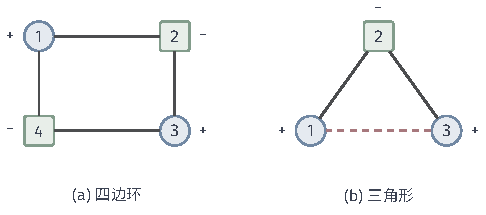
\includegraphics{figures/03-graphs/05-matrices-and-spectra/tikz/incidence-bipartite-signs/figure.pdf}
  \caption{沿环交替分配行符号。圆形顶点保留原行，方形顶点对应的行变号。四边环的每条边都连接异号端点，三角形的虚线边连接两个同号端点。}
  \label{fig:incidence-bipartite-signs}
\end{BookInlineFigure}

\subsection{整数最优解的存在}
\label{sec:incidence-integral-optima}

求最大流时，我们在每个顶点核对流入和流出。求匹配时，在每个顶点数一数选中了几条边。两类问题都是给每条边设一个变量，再用关联矩阵把变量汇总到顶点。如果允许变量取分数值，问题就变成一个普通的线性规划。什么条件能保证放宽后的问题仍有一个整数最优方案？

\subsubsection{关联约束的线性规划}
\label{sec:incidence-lp-models}

把边变量排成向量$\bm{x}$。等式可以规定每个顶点的净流出量，不等式可以限制每条边的容量或每个顶点选边的总量。将等式系数记为$\bm{P}$，上界约束的系数记为$\bm{Q}$，线性松弛可以写成
\begin{equation}
\begin{aligned}
\max_{\bm{x}}\quad &\bm{c}^\top\bm{x}\\
\text{满足}\quad &\bm{P}\bm{x}=\bm{b},\quad
\bm{Q}\bm{x}\leq\bm{d},\quad \bm{x}\geq\bm{0}.
\end{aligned}
\label{eq:incidence-lp-relaxation}
\end{equation}
这里$\bm{b}$和$\bm{d}$是整数数据，$\bm{c}$是目标系数。整数性成立的条件是：把$\bm{P}$和$\bm{Q}$纵向叠在一起得到的矩阵全幺模，并且两个右端都是整数向量。

对每条上界约束，引入一个\term{松弛变量}，记录它还剩多少余量：$\bm{z}=\bm{d}-\bm{Q}\bm{x}\geq\bm{0}$。原来的不等式就等价于$\bm{Q}\bm{x}+\bm{z}=\bm{d}$。把两组等式合在一起，标准型的约束变为
\begin{equation}
\begin{pmatrix}
\bm{P}&\bm{0}\\
\bm{Q}&\bm{I}
\end{pmatrix}
\begin{pmatrix}\bm{x}\\\bm{z}\end{pmatrix}
=
\begin{pmatrix}\bm{b}\\\bm{d}\end{pmatrix},
\qquad \bm{x},\bm{z}\geq\bm{0}.
\label{eq:incidence-lp-slack-matrix}
\end{equation}
每个$\bm{x}$唯一确定一组$\bm{z}$，目标仍为$\bm{c}^\top\bm{x}$。

标准型的系数矩阵右侧多了一个单位阵。看它的任意方子式：如果选中了某个松弛变量的列，这一列在方阵里要么全为零（行列式为零），要么只有一个$1$（沿之展开，阶数降低一）。把选中的松弛列逐一消去，最后剩下的是$\bm{P}$和$\bm{Q}$叠成的矩阵中的一个方子式。如果所有列都是松弛列，消去后空矩阵的行列式按约定等于$1$。因此标准型系数矩阵仍全幺模，右端也仍是整数。

\subsubsection{整数顶点定理}
\label{sec:incidence-integral-vertex-theorem}

把式~\eqref{eq:incidence-lp-slack-matrix}中的原变量和松弛变量合在一起记为$\bm{y}$，右端记为$\bm{r}$，目标系数记为$\bm{a}$（松弛变量的目标系数为零）。标准型变成
\begin{equation}
\max_{\bm{y}}\ \bm{a}^\top\bm{y}
\qquad
\text{满足}\quad \bm{A}\bm{y}=\bm{r},\quad \bm{y}\geq\bm{0}.
\label{eq:incidence-lp-standard}
\end{equation}
线性规划可行且最优值有限时，顶点定理保证最优值能在可行域的某个顶点取得。这里的"顶点"是指不能写成两个不同可行点的凸组合的点。要保证整数最优解存在，只需证明每个顶点的坐标都是整数。顶点定理可参考\BookChapterRef{chap:linear-programming}{卷五"线性规划"章}。

\begin{theorem}[标准型的整数顶点]
\label{thm:graph-tu-integral-vertices}
设式~\eqref{eq:incidence-lp-standard}的系数矩阵$\bm{A}$全幺模，右端$\bm{r}$为整数向量。则可行域的每个顶点都是整数向量。若问题可行且最优值有限，则至少存在一个整数最优解。
\end{theorem}

\begin{proof}
可行域为空时没有顶点需要考察。以下设可行域非空，记$r=\operatorname{rank}\bm{A}$。

先做约化。从$\bm{A}$中选取$r$个线性无关的行，保留对应的右端分量。被删的每一行是所选行的线性组合，把任意可行点代入，可知被删行的右端也是所选右端分量的同一线性组合——因此保留的等式已能推出全部等式。约化后的系数矩阵仍全幺模（方子式只会减少），右端仍为整数。以下继续用$\bm{A}$和$\bm{r}$表示约化后的数据。

若$r=0$，等式约束为空，可行域是$\{\bm{y}\geq\bm{0}\}$。其中每个非零可行点至少有一个正坐标$y_j>0$，沿第$j$个方向正反各动一小步就能把它写成两个不同可行点的中点，所以它不是顶点。只有零向量可能是顶点，它当然是整数向量。以下设$r>0$。

取任意顶点$\bm{y}^\star$，记$S=\{j:y_j^\star>0\}$为正坐标的下标集。我们分三步说明$\bm{y}^\star$为何是整数向量。

第一步：$S$对应的列线性无关。如果相关，就存在非零向量$\bm{h}$，在$S$之外全为零且$\bm{A}\bm{h}=\bm{0}$。取充分小的$\varepsilon>0$使得$\bm{y}^\star\pm\varepsilon\bm{h}$的$S$内坐标仍正，$S$外坐标仍为零。这两个不同的可行点以$\bm{y}^\star$为中点，与顶点定义矛盾。

第二步：将$S$的列补成一组基。$S$对应的独立列数$|S|\leq r$，补选一些列使下标集扩充为$r$列的$J$，令$\bm{A}_J$可逆。$J\setminus S$中的坐标及$J$之外的坐标全为零，因此
\[
\bm{A}_J\bm{y}^\star_J=\bm{r},\qquad \bm{y}^\star_{J^c}=\bm{0}.
\]
$\bm{A}_J$称为\term{基矩阵}，$\bm{y}^\star$是这组基给出的\term{基本可行解}。

第三步：用克莱姆法则求解。$\bm{A}_J$是全幺模矩阵的可逆方形子矩阵，行列式只能为$\pm1$。令$\bm{A}_J^{(i)}$为将$\bm{A}_J$的第$i$列换成$\bm{r}$后的矩阵，克莱姆法则给出
\[
(\bm{y}^\star_J)_i=\frac{\det(\bm{A}_J^{(i)})}{\det(\bm{A}_J)}.
\]
分子是整数矩阵的行列式，本身为整数。分母为$\pm1$。因此每个基坐标都是整数。非基坐标全为零，也是整数。

最后，可行且最优值有限时，由顶点定理取一个最优顶点，它已被证明为整数向量。
\end{proof}

从基矩阵的逆也能看到整数性。由求逆公式，
\[
\bm{A}_J^{-1}=\frac{\operatorname{adj}(\bm{A}_J)}{\det(\bm{A}_J)}.
\]
伴随矩阵$\operatorname{adj}(\bm{A}_J)$的每个条目是一个低一阶的方子式乘以符号，全幺模性保证它们属于$\{0,1,-1\}$。分母为$\pm1$，所以$\bm{A}_J^{-1}$是整数矩阵。用它乘整数右端$\bm{r}$，自然得到整数基坐标。

\subsubsection{图上的整数解}
\label{sec:incidence-integrality-applications}

回到图上的两类问题，分别检查它们的系数矩阵是否满足全幺模条件。

在流量问题里，每个顶点的守恒等式由带符号关联矩阵$\bm{B}$给出，每条弧的容量上界由单位行给出。把$\bm{B}$和$\bm{I}$纵向叠在一起后，任意方子式要么完全来自$\bm{B}$的行列，要么通过沿单位行展开后降阶仍落到$\bm{B}$的子式中。因此堆叠后的矩阵仍全幺模。

在二部匹配问题里，每个顶点的选边额度由无符号关联矩阵$\bm{N}$给出约束$\bm{N}\bm{x}\leq\bm{1}$。每条边恰好连接两个受限的顶点，所以每个$x_e$都被约束在$[0,1]$内。二部图的$\bm{N}$本身已经全幺模（定理~\ref{thm:graph-unsigned-incidence-tu}），松弛变量的单位列不改变全幺模性。

两类问题的右端都是整数，变量都有上界使可行域有界。定理~\ref{thm:graph-tu-integral-vertices}保证只要问题可行，就存在整数最优解。对匹配来说，整数边变量只能取$0$或$1$：$1$表示选中这条边，$0$表示不选。

最大流的流值$F$本身也是变量。图~\ref{fig:incidence-flow-integer-example}展示了一种处理方式：添加一条回流弧$t\to s$，使回流弧的流量$q_4$等于原网络的流值。加上回流弧后，每个顶点（包括源和汇）的守恒式都取零右端。目标就是最大化回流弧上的流量。删去回流弧就还原原图中的流。图中的三点网络里，中转路线$s\to a\to t$受容量$1$限制，直达路线$s\to t$的容量也是$1$，两条各运一个单位，达到最大流值$2$。如果是给定整数供需的最小费用流，则直接以指定的净流出量作为右端。

\begin{BookInlineFigure}
\centering
\begin{tikzpicture}[
  x=1.16cm, y=1cm,
  point/.style={circle,draw=incFlowBlue,fill=incFlowLight,
    minimum size=6mm,inner sep=0pt,line width=.75pt},
  arc/.style={-{Stealth[length=2.2mm]},draw=incFlowLine,line width=.85pt}
]
\definecolor{incFlowBlue}{HTML}{7188A3}
\definecolor{incFlowLight}{HTML}{E5EAF0}
\definecolor{incFlowLine}{HTML}{4C4D4F}
\definecolor{incFlowGreen}{HTML}{829C8B}
\node[point] (s) at (0,0) {$s$};
\node[point] (a) at (2,1.13) {$a$};
\node[point] (t) at (4,0) {$t$};
\draw[arc] (s) -- node[above left] {$q_1\;(2)$} (a);
\draw[arc] (a) -- node[above right] {$q_2\;(1)$} (t);
\draw[arc] (s) -- node[above] {$q_3\;(1)$} (t);
\draw[arc,draw=incFlowGreen,dashed] (t) to[bend left=26]
  node[below] {$q_4\;(3)$} (s);
\end{tikzpicture}

\caption{三点最大流网络。实线标出三条原有弧，括号内是容量。虚线是为守恒记账加上的回流弧，其流量$q_4$等于原网络的流值。}
\label{fig:incidence-flow-integer-example}
\end{BookInlineFigure}

图~\ref{fig:incidence-matching-comparison}对照了全幺模条件成立和失效时的选边方案。

在四边环上，两个交替选边的整数方案各选两条不相邻的边，总量为$2$。四条边各取$1/2$是这两个方案的平均，也达到最优值$2$。这说明整数最优解与分数最优点可以并存。

在三角形上，每条边取$1/2$恰好用满三个顶点的额度，总量为$3/2$。把三个约束$x_{12}+x_{23}\leq1$、$x_{12}+x_{13}\leq1$、$x_{23}+x_{13}\leq1$相加并除以$2$，可知$3/2$已经是松弛问题的上界。而整数匹配最多选一条边，最优值只有$1$。这个间隙的来源正是三角形的无符号关联矩阵行列式为$2$——克莱姆法则中的除法产生了$1/2$。

\begin{BookInlineFigure}
  \centering
  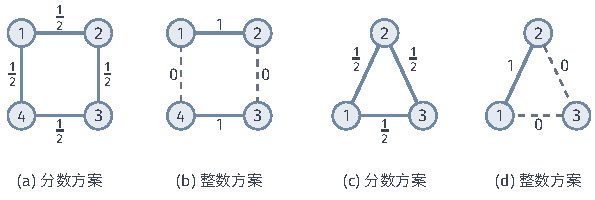
\includegraphics{figures/03-graphs/05-matrices-and-spectra/tikz/incidence-matching-comparison/figure.pdf}
  \caption{四边环和三角形上的选边方案。每个顶点周围的选边量之和都不超过$1$。边旁的数是选边量，实线表示该量为正，虚线表示为零。(a)、(b) 的总量均为$2$，(c)、(d) 分别为$3/2$和$1$。}
  \label{fig:incidence-matching-comparison}
\end{BookInlineFigure}

具体的求解方法见第~\ref{chap:max-flow-min-cut}章、第~\ref{chap:min-cost-flow}章和第~\ref{chap:bipartite-matching-assignment}章。
\section{本章小结}
\label{sec:graph-incidence-summary}

给定参考方向后，图的带符号关联矩阵$\bm{B}\in\mathbb{R}^{n\times m}$在第$e$列（对应有向边$e\colon u\to v$）于尾端$u$记$+1$、头端$v$记$-1$，把顶点函数空间$\mathbb{R}^V$与边空间$\mathbb{R}^E$连接成一对伴随映射：转置矩阵$\bm{B}^\top\colon\mathbb{R}^V\to\mathbb{R}^E$将顶点函数$\bm{f}$映射为沿边差分向量$\bm{d}=\bm{B}^\top\bm{f}$，矩阵本身$\bm{B}\colon\mathbb{R}^E\to\mathbb{R}^V$将边流量向量$\bm{q}$映射为各顶点的净流出向量$\bm{B}\bm{q}$，二者满足伴随恒等式$\langle\bm{B}^\top\bm{f},\bm{q}\rangle_E=\langle\bm{f},\bm{B}\bm{q}\rangle_V$。

在边空间$\mathbb{R}^E$中，每个顶点处净流出量均为零的边流量构成环空间$\mathcal{C}(\mathcal{G})=\ker\bm{B}$，能够表示为顶点函数沿边差分向量的边向量构成割空间$\mathcal{D}(\mathcal{G})=\operatorname{im}\bm{B}^\top$。由伴随恒等式，环空间与割空间正交互补，将边空间正交直和分解为$\mathbb{R}^E=\ker\bm{B}\oplus\operatorname{im}\bm{B}^\top$。

若图有$n$个顶点、$m$条边和$c$个连通分量，则$\ker\bm{B}^\top$由$c$个连通分量的指示向量张成且线性无关，维数为$c$；由秩零度定理，关联矩阵的秩与割空间维数均为$n-c$，环空间维数为$m-n+c$。

选定一棵生成森林$F$后，向$F$中逐一添入$m-n+c$条非树边得到环空间的基本环基（在非树边坐标上构成单位阵），从$F$中逐一删去$n-c$条树边得到割空间的基本割基（在树边坐标上构成单位阵）。

在组合优化中，若整数矩阵的任意阶方子式均属于$\{0,1,-1\}$，则称之为全幺模矩阵。在标准型线性规划中，全幺模系数矩阵与整数右端项使可行域的每个可逆基矩阵行列式均为$\pm1$，由克莱姆法则保证所有极点（基本可行解）均为整数向量，当问题可行且最优值有限时，便存在整数最优解。

按约束矩阵类型划分：以带符号关联矩阵$\bm{B}$为约束的有向网络流家族（最小费用流、最大流、最短路），因$\bm{B}$每列恰有一正一负、对任意无自环图恒全幺模，故在整数供需与容量、问题可行且最优值有限时存在整数最优流；最短路的单位流模型还须排除负费用环。

以无符号关联矩阵$\bm{N}$为约束的配对与覆盖家族（最大匹配、指派问题、最小顶点覆盖），因$\bm{N}$每列有两个$+1$、当且仅当图为不含奇环的二部图时全幺模（奇环子矩阵的排列展开给出行列式$1+1=2$），故在二部图上保证存在$\{0,1\}$整数最优解，而在含奇环图上会出现分数极点。

后续章节将频繁使用本章建立的关联矩阵框架。将沿边差分算子$\bm{B}^\top$、非负边权对角矩阵$\bm{C}$与净流出汇总算子$\bm{B}$依次复合，得到顶点空间上的对称半正定算子$\bm{L}=\bm{B}\bm{C}\bm{B}^\top$——这正是第~\ref{chap:graph-laplacian-matrix}章的组合拉普拉斯矩阵，并在第~\ref{chap:graph-electrical-networks}章的电网络方程中把电势差、支路电导与基尔霍夫电流守恒融为一体。


\chapter{邻接矩阵}
\label{chap:graph-adjacency-matrix}

在四个顶点组成的四元环上添一条对角线，图中就出现两个三角形。如果手里只有这张图的邻接矩阵特征值，还能数出这两个三角形吗？

答案是可以：把全部特征值各自立方后相加，再除以$6$，就得到三角形的个数。这个公式之所以成立，是因为邻接矩阵的三次幂记录了图中所有三步行走的条数，而在简单无向图中，走三步回到起点的闭行走恰好就是绕某个三角形走一圈（三个起点、顺逆两个方向共给出$6$条闭行走）。更一般地，邻接矩阵$k$次幂的第$(u,v)$个元素$(\bm A^k)_{u,v}$等于从顶点$u$到顶点$v$的$k$步行走条数。

本章围绕邻接矩阵的谱展开，按“谱是什么——典型图怎么算——谱本身有什么性质——能从谱读出什么图结构——谱和商谱丢失了什么信息”的脉络推进。第~\ref{sec:adjacency-walk-counts}节从行走计数出发，建立矩阵幂、迹与谱矩之间的基本联系。第~\ref{sec:adjacency-standard-spectra}节在完全图、完全二部图、环、路径、笛卡儿积图与正则补图上直接构造特征向量，提供一组可随时检验的基准谱。

第~\ref{sec:adjacency-spectral-properties}节研究邻接谱自身的结构性质：连通图最大特征值的单根性与正特征向量、平均度与最大度夹逼界、子图单调性，以及二部图谱关于原点的正负对称。

第~\ref{sec:adjacency-spectral-structure}节利用谱信息刻画图结构：先由低阶谱矩读出边数与三角形数，并说明四环计数还需度信息，再由特征值限制图的直径、色数和独立数，并通过同谱图反例指出完整谱的信息边界。

最后，第~\ref{sec:adjacency-spectral-invariant}节引入等价划分与颜色细化导出的公平划分，证明商谱精确嵌入完整邻接谱，并比较商谱保留的宏观块结构与丢失的块内微观细节\scite{brouwer2012spectra}。

沿用第~\ref{sec:graph-conn-adjacency-matrix}节的记号。在图$\mathcal G=(V,E)$中，$V$是顶点集，$E$是边集，记$n=|V|$为顶点数、$m=|E|$为边数。除特别说明外，本章讨论非空有限简单无向图（无自环、无重边）。

固定顶点排列次序$1,2,\ldots,n$后，$n\times n$邻接矩阵$\bm A=(a_{i,j})$定义为：若顶点$i$与$j$之间有边，则$a_{i,j}=1$；否则$a_{i,j}=0$。无向图的边没有方向，$a_{i,j}=a_{j,i}$，因此$\bm A$是实对称矩阵。实对称矩阵必有$n$个实特征值，将它们按降序排列为
\[
\lambda_1\geq\lambda_2\geq\cdots\geq\lambda_n,
\]
重根按代数重数重复计入，所成多重集称为图$\mathcal G$的\term{邻接谱}（adjacency spectrum）。

当图带有非负边权时，用$w_{i,j}=w_{j,i}\geq 0$记录连接顶点$i,j$的边权（不相邻的顶点对及对角元取$w_{i,j}=0$），构成$n\times n$非负实对称加权邻接矩阵$\bm W=(w_{i,j})$；简单无权图的邻接矩阵$\bm A$正是每条边权取$1$的特例。

\section{邻接矩阵的谱}
\label{sec:adjacency-walk-counts}

邻接矩阵记录哪些顶点直接相连。乘一次矩阵，相当于沿边走一步。多乘几次，就能数出不同长度的行走。如果只看那些走完又回到起点的行走，把各起点的数目相加，总数恰好是矩阵幂的迹——而迹可以用特征值直接算出来。

我们先从一步开始，看矩阵乘法怎样对应到行走的拼接。

从顶点$u$出发，走一步能到达哪些顶点？如果$u$和$v$之间有边，恰好有一种走法；如果没有边，走不过去。邻接矩阵的元素$a_{u,v}$就记录了这个数：有边时为$1$，无边时为$0$。换句话说，$(\bm A^1)_{u,v}=a_{u,v}$恰好等于从$u$到$v$的一步行走条数。

现在考虑两步行走。以路径$1\text{--}2\text{--}3$为例。从顶点$1$出发，第一步只能到$2$（因为$1$只和$2$相邻），第二步可以回到$1$或继续到$3$。两种走法分别是$1\to2\to1$和$1\to2\to3$。

写成矩阵乘法来看：$\bm A^2$的第$(1,3)$项是
\[
(\bm A^2)_{1,3}=\sum_{z\in V}a_{1,z}\,a_{z,3}.
\]
求和中的$z$跑遍所有顶点。只有$z=2$同时满足$a_{1,z}=1$和$a_{z,3}=1$，其余项都包含一个零因子。所以$(\bm A^2)_{1,3}=1$，正好等于从$1$经过一个中间点到$3$的行走条数。

这不是巧合。每一项$a_{1,z}\cdot a_{z,3}$恰好在$1$和$z$之间有边、同时$z$和$3$之间也有边时等于$1$，否则为零。也就是说，每一项对应一种中间顶点$z$的选择。把所有选择加起来，就是把所有可能的中间点$z$的行走都数到了。

图~\ref{fig:adjacency-walk-progression}用四点环加对角线$\{1,3\}$的例子，逐步展示从顶点$1$出发走$k=1,2,3$步能到达各点的行走条数，也就是$\bm A^k$第一行的各个元素。观察三个面板：一步只能到达$1$的直接邻居，二步可以经一个中间点到达更远的顶点（包括返回自身），三步则出现了更多走法。$(\bm A^3)_{1,1}=4$说明从$1$走三步回到$1$有四条不同的路线。

\begin{figure}[!htb]
\centering
\begin{tikzpicture}[x=1mm,y=1mm,>=Stealth,
  vertex/.style={circle,draw=FigureBlue,fill=FigureBlueFill,inner sep=0pt,
    minimum size=5mm,line width=.52pt,font=\figurefont\fontsize{8}{10}\selectfont},
  origin/.style={vertex,fill=FigureYellowFill,draw=FigureYellow,line width=.72pt},
  countlabel/.style={font=\figurefont\fontsize{7.5}{9}\selectfont,FigureInk},
  panel/.style={anchor=mid,font=\figurefont\footnotesize}]
  % Panel (a): k=1, A^1 row 1 = (0,1,1,1)
  \begin{scope}[xshift=0mm]
    \node[origin] (a1) at (0,12) {$1$};
    \node[vertex] (a2) at (12,12) {$2$};
    \node[vertex] (a3) at (12,0) {$3$};
    \node[vertex] (a4) at (0,0) {$4$};
    \draw[FigureStroke,line width=.45pt] (a1)--(a2) (a2)--(a3) (a3)--(a4) (a4)--(a1) (a1)--(a3);
    \draw[->,FigureBlue,line width=.7pt] (a1) -- (a2);
    \draw[->,FigureBlue,line width=.7pt] (a1) -- (a3);
    \draw[->,FigureBlue,line width=.7pt] (a1) -- (a4);
    \node[countlabel,above] at (a1.north) {$0$};
    \node[countlabel,above] at (a2.north) {$1$};
    \node[countlabel,below] at (a3.south) {$1$};
    \node[countlabel,below] at (a4.south) {$1$};
    \node[panel] at (6,-8) {(a) $k=1$};
  \end{scope}
  % Panel (b): k=2, A^2 row 1 = (3,1,2,1)
  \begin{scope}[xshift=36mm]
    \node[origin] (b1) at (0,12) {$1$};
    \node[vertex] (b2) at (12,12) {$2$};
    \node[vertex] (b3) at (12,0) {$3$};
    \node[vertex] (b4) at (0,0) {$4$};
    \draw[FigureStroke,line width=.45pt] (b1)--(b2) (b2)--(b3) (b3)--(b4) (b4)--(b1) (b1)--(b3);
    \node[countlabel,above] at (b1.north) {$3$};
    \node[countlabel,above] at (b2.north) {$1$};
    \node[countlabel,below] at (b3.south) {$2$};
    \node[countlabel,below] at (b4.south) {$1$};
    \node[panel] at (6,-8) {(b) $k=2$};
  \end{scope}
  % Panel (c): k=3, A^3 row 1 = (4,3,4,3)
  \begin{scope}[xshift=72mm]
    \node[origin] (c1) at (0,12) {$1$};
    \node[vertex] (c2) at (12,12) {$2$};
    \node[vertex] (c3) at (12,0) {$3$};
    \node[vertex] (c4) at (0,0) {$4$};
    \draw[FigureStroke,line width=.45pt] (c1)--(c2) (c2)--(c3) (c3)--(c4) (c4)--(c1) (c1)--(c3);
    \node[countlabel,above] at (c1.north) {$4$};
    \node[countlabel,above] at (c2.north) {$3$};
    \node[countlabel,below] at (c3.south) {$4$};
    \node[countlabel,below] at (c4.south) {$3$};
    \node[panel] at (6,-8) {(c) $k=3$};
  \end{scope}
\end{tikzpicture}
\caption{四点环加对角线$\{1,3\}$上，从顶点$1$出发走$k$步到达各顶点的行走条数，即$\bm A^k$第一行的各个元素。浅黄色标出起点$1$。(a) 一步只能到达三个邻居。(b) 两步后可以到达自身（三条往返路线），也能经过中间顶点到达$3$（两条路线）。(c) 三步后各点的行走数继续增长。}
\label{fig:adjacency-walk-progression}
\end{figure}

\paragraph{从一步到多步}

这个思路推广到$k$步行走。设我们已经知道$(\bm A^k)_{u,z}$等于从$u$到$z$的$k$步行走条数。现在要数从$u$到$v$的$k+1$步行走。

任取一条这样的行走$u=v_0\to v_1\to\cdots\to v_k\to v_{k+1}=v$。倒数第二个顶点$z=v_k$把这条行走唯一地拆成两段：前$k$步从$u$到$z$，最后一步从$z$到$v$。

反过来，对每个与$v$相邻的顶点$z$，把任意一条从$u$到$z$的$k$步行走接上最后一步$z\to v$，就拼出一条从$u$到$v$的$k+1$步行走。不同的$z$或不同的前段行走拼出的是不同的$k+1$步行走。

把所有中间点$z$的贡献相加：从$u$到$z$有$(\bm A^k)_{u,z}$条$k$步行走，其中每一条都可以接上最后一步$z\to v$，而最后一步能否走取决于$a_{z,v}$是否为$1$。因此
\[
\text{从$u$到$v$的$k+1$步行走数}
=\sum_{z\in V}(\bm A^k)_{u,z}\,a_{z,v}.
\]
右边按矩阵乘法的定义，正是$(\bm A^{k+1})_{u,v}$。综合以上推理，我们得到

\begin{theorem}[行走计数]
\label{thm:adjacency-walk-count}
设$\bm A$是简单无向图的邻接矩阵。对任意正整数$k$和任意一对顶点$u,v$，
\begin{equation}
(\bm A^k)_{u,v}=\text{从$u$到$v$的$k$步行走条数。}
\label{eq:adjacency-walk-count}
\end{equation}
\end{theorem}

\paragraph{闭行走与迹}

一条从$u$出发又回到$u$的行走叫作\term{闭行走}（closed walk）。在定理~\ref{thm:adjacency-walk-count}中取$v=u$，从$u$出发的$k$步闭行走数就是对角元$(\bm A^k)_{u,u}$。

把所有$k$步闭行走按起点分组。每条闭行走有唯一的第一个顶点，因此恰好属于一组。第$u$组有$(\bm A^k)_{u,u}$条记录。把各组加起来，
\begin{equation}
\text{$k$步闭行走总数}
=\sum_{u\in V}(\bm A^k)_{u,u}
=\operatorname{tr}(\bm A^k).
\label{eq:adjacency-closed-walk-trace}
\end{equation}

回到路径$1\text{--}2\text{--}3$的例子。从顶点$1$出发，两步回来只有$1\to2\to1$一条。从顶点$2$出发，有$2\to1\to2$和$2\to3\to2$两条。从顶点$3$出发，只有$3\to2\to3$一条。三个对角元依次是$1,2,1$，迹为$4$。行走$1\to2\to3$没有回到起点，记录在非对角项$(\bm A^2)_{1,3}$中，不计入迹。

起点是闭行走的一部分。沿三角形$1\to2\to3\to1$走一圈，换个起点就变成$2\to3\to1\to2$或$3\to1\to2\to3$，三条记录分别计入三个不同的对角元。

闭行走允许重复经过顶点和边。例如在只有一条边$\{a,b\}$的图上，$a\to b\to a$是两步闭行走，$a\to b\to a\to b\to a$是四步闭行走，两者都反复使用同一条边。只有在途中各顶点互不重复、最后一步回到起点、且长度至少为三时，才形成简单环。

\paragraph{迹与谱矩}

上面的结论把行走计数和矩阵幂联系在一起。下面再把矩阵幂的迹接到特征值上。

$\bm A$是实对称矩阵，因此有一组正交特征向量基$\bm u_1,\ldots,\bm u_n$和对应的实特征值$\lambda_1,\ldots,\lambda_n$。将这组基排成正交矩阵$\bm P$，可以写成$\bm A=\bm P\operatorname{diag}(\lambda_1,\ldots,\lambda_n)\bm P^\top$。

把$\bm A$乘$k$次。由于$\bm P^\top\bm P=\bm I$，相邻两个$\bm A$之间的$\bm P^\top$和$\bm P$互相抵消，只留下
\[
\bm A^k=\bm P\operatorname{diag}(\lambda_1^k,\ldots,\lambda_n^k)\bm P^\top.
\]
在特征基下，$\bm A^k$的对角元就是$\lambda_1^k,\ldots,\lambda_n^k$。

迹是对角元之和。换基不改变迹——准确地说，$\operatorname{tr}(\bm P\bm D\bm P^\top)=\operatorname{tr}(\bm D\bm P^\top\bm P)=\operatorname{tr}(\bm D)$，用到的是迹的循环性质$\operatorname{tr}(\bm X\bm Y)=\operatorname{tr}(\bm Y\bm X)$。因此
\begin{equation}
\operatorname{tr}(\bm A^k)=\sum_{i=1}^{n}\lambda_i^k,
\qquad k=1,2,\ldots .
\label{eq:adjacency-spectral-moments}
\end{equation}

\begin{definition}[邻接谱与谱矩]
\label{def:adjacency-spectrum}
设$\bm A$是$n$阶实对称邻接矩阵，$\lambda_1\ge\cdots\ge\lambda_n$为其特征值（按降序排列，重复的按重数计入）。全部特征值组成的多重集$\{\lambda_1,\ldots,\lambda_n\}$称为图的\term{邻接谱}（adjacency spectrum）。和$\sum_{i=1}^n\lambda_i^k$称为第$k$阶\term{谱矩}（spectral moment）。
\end{definition}

这样，我们有了一条从图结构到代数运算的路线：矩阵幂数行走，对角元数闭行走，迹把所有起点加起来，而谱矩只用特征值就能算出迹。后续各节将分别回答：典型图的特征值是什么（第~\ref{sec:adjacency-standard-spectra}节），谱本身有什么结构性质（第~\ref{sec:adjacency-spectral-properties}节），以及谱能够或不能够告诉我们哪些图的结构信息（第~\ref{sec:adjacency-spectral-structure}节和第~\ref{sec:adjacency-spectral-invariant}节）。

若改用带权矩阵$\bm W$，矩阵乘法的每一步都乘上对应边的权重。一条行走对$(\bm W^k)_{u,v}$的贡献不再是$1$，而是沿途$k$条边权重的乘积。一条边被走了几次，它的权重就乘几次。此时迹累计的是所有闭行走的权重和；取单位权时退化为闭行走条数。


\section{典型图的谱}
\label{sec:adjacency-standard-spectra}

上一节建立了闭行走计数与谱矩的一般联系。在研究一般图的谱性质之前，我们先问一个具体问题：对于完全图、完全二部图、环、路径、笛卡儿积图和正则补图这些结构高度对称或规则的图族，能否不解高次特征多项式，直接通过观察邻接矩阵对顶点赋值的作用构造出全部$n$个特征向量与特征值？

本节依次计算这几类典型图的完整邻接谱。它们不仅展示了利用对称性、周期边界和张量积分解求谱的基本技巧，也为后续各节检验谱界与构造反例提供了标准算例。

\subsection{完全图与完全二部图}
\label{sec:adjacency-complete-spectra}

完全图和完全二部图的共同特点是：同一类顶点的邻居集合几乎完全一致，因此邻接矩阵可以用全一矩阵$\bm J$或秩一分块矩阵简洁表示。

\paragraph{完全图}

在$n$个顶点的完全图$K_n$中，每个顶点都与除自身以外的其余$n-1$个顶点相邻。记$\bm 1=(1,\ldots,1)^\top\in\mathbb R^n$为全一列向量，$\bm J=\bm 1\bm 1^\top\in\mathbb R^{n\times n}$为全一矩阵，则$K_n$的邻接矩阵可以写为
\[
\bm A=\bm J-\bm I.
\]
这个分解式清楚地说明了$\bm A$对任意顶点向量$\bm x\in\mathbb R^n$的作用：因为$\bm J\bm x=\bm 1(\bm 1^\top\bm x)=\bigl(\sum_{j=1}^n x_j\bigr)\bm 1$，左乘$\bm J$相当于先把所有顶点的读数加成一个总和，再把这个总和复制到每一个顶点上；减去$\bm I\bm x=\bm x$则是从全图总和中扣掉每个顶点自身的读数，剩下的自然就是其余$n-1$个邻居的读数之和。

利用$\bm A=\bm J-\bm I$，可以直接在两个正交互补的子空间上读出全部特征向量。首先是$1$维常向量方向：取全一向量$\bm x=\bm 1$，由于$\bm J\bm 1=n\bm 1$，有
\[
\bm A\bm 1=(\bm J-\bm I)\bm 1=(n-1)\bm 1,
\]
因此$\bm 1$是属于特征值$\lambda_1=n-1$的特征向量，张成一个$1$维特征子空间。

其次考察与$\bm 1$正交的$n-1$维零和子空间
\[
\bm 1^\perp=\Bigl\{\bm x\in\mathbb R^n:\bm 1^\top\bm x=\sum_{j=1}^n x_j=0\Bigr\}.
\]
由于只有一个线性齐次约束$\sum_{j=1}^n x_j=0$，$\bm 1^\perp$的维数为$n-1$。对任意非零向量$\bm x\in\bm 1^\perp$，全图读数总和$\bm 1^\top\bm x=0$，故$\bm J\bm x=\bm 1(\bm 1^\top\bm x)=\bm 0$，从而
\[
\bm A\bm x=(\bm J-\bm I)\bm x=\bm 0-\bm x=-\bm x.
\]
这说明零和子空间$\bm 1^\perp$中的每一个非零向量都是$\bm A$属于特征值$-1$的特征向量。例如在三角形$K_3$上取$\bm x=(1,-1,0)^\top\in\bm 1^\perp$，顶点$1$的两个邻居读数之和为$(-1)+0=-1=-x_1$，其余两个顶点同理。常向量方向（$1$维）与零和子空间$\bm 1^\perp$（$n-1$维）正交直和构成整个$\mathbb R^n$（$1+(n-1)=n$），因此我们已经找齐了$K_n$的全部特征值。

\begin{theorem}[完全图的邻接谱]
\label{prop:adjacency-complete-spectrum}
$n$个顶点的完全图$K_n$（$n\geq 2$）的邻接特征值为$n-1$（重数$1$，对应常向量$\bm 1$）和$-1$（重数$n-1$，对应零和子空间$\bm 1^\perp$）。
\end{theorem}

可以用前两阶谱矩快速核对：特征值之和为$(n-1)+(n-1)(-1)=0=\operatorname{tr}(\bm A)$；特征值平方和为$(n-1)^2+(n-1)(-1)^2=n(n-1)=2\binom{n}{2}=2m=\operatorname{tr}(\bm A^2)$。

\paragraph{完全二部图}

完全二部图$K_{p,q}$的顶点集划分为左右两部分$U$和$W$，其中$|U|=p,|W|=q$，总顶点数为$n=p+q$。同侧顶点之间没有任何边，左侧每个顶点都与右侧全部$q$个顶点相邻，右侧每个顶点都与左侧全部$p$个顶点相邻。按先排$U$中$p$个顶点、再排$W$中$q$个顶点的顺序，邻接矩阵具有分块形式
\[
\bm A=
\begin{pmatrix}
\bm 0_{p\times p} & \bm 1_p\bm 1_q^\top\\
\bm 1_q\bm 1_p^\top & \bm 0_{q\times q}
\end{pmatrix}.
\]
对任意分块向量$\bm x=\binom{\bm x_U}{\bm x_W}$（其中$\bm x_U\in\mathbb R^p,\bm x_W\in\mathbb R^q$），邻接矩阵的作用是：将右侧分量之和$\bm 1_q^\top\bm x_W$赋给左侧的每一个顶点，同时将左侧分量之和$\bm 1_p^\top\bm x_U$赋给右侧的每一个顶点：
\[
\bm A\begin{pmatrix}\bm x_U\\\bm x_W\end{pmatrix}
=\begin{pmatrix}(\bm 1_q^\top\bm x_W)\bm 1_p\\(\bm 1_p^\top\bm x_U)\bm 1_q\end{pmatrix}.
\]

根据这一作用机制，我们按“两侧各自取常值”和“两侧各自零和”分两步找出全部$p+q$个特征方向。

先看$2$维的两侧常值方向：由于$\bm A$的输出在$U$侧和$W$侧内部总是常值，任何非零特征值$\lambda\neq 0$对应的特征向量必定在$U$侧取某个常数$a$、在$W$侧取某个常数$b$，即$\bm x=\binom{a\bm 1_p}{b\bm 1_q}$。此时左侧每个顶点有$q$个读数为$b$的右侧邻居，邻居和为$qb$；右侧每个顶点有$p$个读数为$a$的左侧邻居，邻居和为$pa$。特征方程$\bm A\bm x=\lambda\bm x$化为二元线性方程组
\[
qb=\lambda a,\qquad pa=\lambda b.
\]
将第一式$b=\lambda a/q$代入第二式，得$pa=\lambda^2 a/q$，因$(a,b)\neq(0,0)$，解得
\[
\lambda^2=pq,\qquad\text{即}\qquad \lambda=\pm\sqrt{pq}.
\]
当$\lambda=+\sqrt{pq}$时，$a/b=\sqrt{q/p}$，可取同号特征向量$(a,b)=(\sqrt{q},\sqrt{p})$；当$\lambda=-\sqrt{pq}$时，$a/b=-\sqrt{q/p}$，可取异号特征向量$(a,b)=(\sqrt{q},-\sqrt{p})$。这两个方向线性无关，共给出$2$个非零特征值$\pm\sqrt{pq}$。

再看$p+q-2$维的两侧零和子空间：若分块向量$\bm x=\binom{\bm x_U}{\bm x_W}$在左侧的读数总和为零（$\bm 1_p^\top\bm x_U=0$）且在右侧的读数总和也为零（$\bm 1_q^\top\bm x_W=0$），则由上面的分块作用公式立得$\bm A\bm x=\bm 0$，即$\bm x$是属于特征值$0$的特征向量。左侧零和条件$\bm 1_p^\top\bm x_U=0$留出$p-1$个独立方向，右侧零和条件$\bm 1_q^\top\bm x_W=0$留出$q-1$个独立方向，两侧直接拼合共给出$(p-1)+(q-1)=p+q-2$维零空间。两类子空间维数之和为$2+(p+q-2)=p+q=n$，覆盖了整个顶点空间。

\begin{theorem}[完全二部图的邻接谱]
\label{prop:adjacency-bipartite-complete-spectrum}
完全二部图$K_{p,q}$（$p,q\geq 1$）的邻接特征值为$\sqrt{pq}$（重数$1$）、$-\sqrt{pq}$（重数$1$）以及$0$（重数$p+q-2$）。
\end{theorem}

以五顶点星图$K_{1,4}$（$p=1$个中心点连接$q=4$个叶子点）为例：$\sqrt{pq}=\sqrt{1\times 4}=2$，零特征值重数为$1+4-2=3$，故完整邻接谱为$\{2,0,0,0,-2\}$。第~\ref{sec:adjacency-cospectral-graphs}节将用它与不连通图$C_4\sqcup K_1$构造同谱非同构图。同时可以看到，$K_{p,q}$的正负特征值$\pm\sqrt{pq}$成对对称出现——第~\ref{sec:adjacency-bipartite-symmetry}节将证明这是所有二部图的普遍性质。

\subsection{环与路径}
\label{sec:adjacency-cycle-path-spectra}

完全图和完全二部图的特征向量依靠“整块取常值”构造，而环$C_n$与路径$P_n$的每个顶点只和左右相邻顶点相连，其特征向量表现为沿顶点编号周期性起伏的复指数波或正弦驻波。

\paragraph{环}

将$n$点环$C_n$（$n\ge3$）的顶点沿圆周依次编号为$0,1,\ldots,n-1$（模$n$同余，使得第$n$个位置回到顶点$0$）。对每个顶点$j$，它的两个邻居是$j-1$和$j+1$，因此邻接矩阵$\bm A$的第$j$行作用在向量$\bm z=(z_0,z_1,\ldots,z_{n-1})^\top$上就是把左右两个邻居的值相加：
\[
(\bm A\bm z)_j=z_{j-1}+z_{j+1},\qquad j=0,1,\ldots,n-1\pmod n.
\]

由于图在顶点编号循环移位$j\mapsto j+1$下具有平移对称性，我们尝试幂函数形式的向量$z_j=\omega^j$（$\omega\in\mathbb C\setminus\{0\}$）。代入邻居和公式，左移一步乘以$\omega^{-1}$、右移一步乘以$\omega$，公共因子$\omega^j=z_j$直接提出来：
\[
(\bm A\bm z)_j=\omega^{j-1}+\omega^{j+1}=(\omega^{-1}+\omega)\omega^j=(\omega^{-1}+\omega)z_j.
\]
为了让$\bm z$在绕环一圈后首尾衔接无歧义，第$n$个位置的值必须等于第$0$个位置的值，即周期边界条件
\[
z_n=z_0\quad\Longleftrightarrow\quad \omega^n=1.
\]
方程$\omega^n=1$在复平面单位圆上恰有$n$个不同的$n$次单位根：
\[
\omega_k=\exp\Bigl(\frac{2\pi\mathrm ik}{n}\Bigr)=\cos\frac{2\pi k}{n}+\mathrm i\sin\frac{2\pi k}{n},
\qquad k=0,1,\ldots,n-1.
\]
对每个$k$，由于$\omega_k^{-1}=\exp(-2\pi\mathrm ik/n)=\cos(2\pi k/n)-\mathrm i\sin(2\pi k/n)$，对应的特征值为
\begin{equation}
\lambda_k=\omega_k^{-1}+\omega_k=2\cos\Bigl(\frac{2\pi k}{n}\Bigr),
\qquad k=0,1,\ldots,n-1.
\label{eq:adjacency-cycle-spectrum}
\end{equation}
当$k\neq\ell$时，$\omega_k^{-1}\omega_\ell=\exp(2\pi\mathrm i(\ell-k)/n)\neq 1$是异于$1$的$n$次单位根，由等比数列求和知两个模式向量的复内积为$\sum_{j=0}^{n-1}(\omega_k^{-1}\omega_\ell)^j=0$。因此这$n$个单位根模式向量两两正交、线性无关，式~\eqref{eq:adjacency-cycle-spectrum}给出了$C_n$的全部$n$个特征值。

\begin{theorem}[环的邻接谱]
\label{prop:adjacency-cycle-spectrum}
$n$个顶点的环$C_n$（$n\ge3$）的邻接特征值为
\[
\lambda_k=2\cos\Bigl(\frac{2\pi k}{n}\Bigr),
\qquad k=0,1,\ldots,n-1.
\]
\end{theorem}

虽然推导中借用了复指数向量$\bm z^{(k)}$，但由于$\cos(2\pi(n-k)/n)=\cos(2\pi k/n)$，共轭模式$k$与$n-k$具有相同的实特征值$\lambda_k$；当模式不为实数时，取$\bm z^{(k)}$的实部和虚部，得到实数域上的余弦特征向量$\cos(2\pi kj/n)$与正弦特征向量$\sin(2\pi kj/n)$。例如在四元环$C_4$上，$k=0,1,2,3$给出特征值$2,0,-2,0$（降序排列为$2,0,0,-2$），其中重数为$2$的特征值$0$对应两个正交实特征向量$(1,0,-1,0)^\top$和$(0,1,0,-1)^\top$。

\paragraph{路径}

先设$n\geq2$。$n$个顶点的路径$P_n$（顶点依次编号为$1,2,\ldots,n$）与环$C_n$的唯一区别在于两端边界：内部顶点$j\in\{2,\ldots,n-1\}$各有左右两个邻居$j-1$和$j+1$，而左端点$1$只有右邻居$2$，右端点$n$只有左邻居$n-1$：
\[
(\bm A\bm x)_1=x_2,\qquad
(\bm A\bm x)_j=x_{j-1}+x_{j+1}\quad(2\leq j\leq n-1),\qquad
(\bm A\bm x)_n=x_{n-1}.
\]

怎样让两个端点也能套用内部顶点的统一公式$x_{j-1}+x_{j+1}$？只需在路径左端外侧添一个虚拟顶点$0$、在右端外侧添一个虚拟顶点$n+1$，并强制要求这两个虚拟位置上的读数为零：
\[
x_0=0,\qquad x_{n+1}=0.
\]
一旦加上这两个零边界条件，左端点$j=1$处的$x_0+x_2$就自动退化为$x_2$，右端点$j=n$处的$x_{n-1}+x_{n+1}$就自动退化为$x_{n-1}$。于是整条路径的特征方程$\bm A\bm x=\lambda\bm x$完全等价于：寻找不全为零的序列$x_0,x_1,\ldots,x_{n+1}$，使其同时满足递推关系与两端零边界条件：
\[
x_{j-1}+x_{j+1}=\lambda x_j\quad(1\leq j\leq n),
\qquad x_0=0,\quad x_{n+1}=0.
\]

为自动满足左端零边界条件$x_0=0$，我们试取正弦驻波模式
\[
x_j=\sin(j\theta),\qquad j=0,1,\ldots,n+1,
\]
其中$\theta\in(0,\pi)$为待定角频率。显然$x_0=\sin 0=0$恒成立。对任意$1\leq j\leq n$，利用三角函数的和差化积公式展开左右邻居之和：
\[
x_{j-1}+x_{j+1}
=\sin\bigl((j-1)\theta\bigr)+\sin\bigl((j+1)\theta\bigr)
=2\cos\theta\,\sin(j\theta)
=(2\cos\theta)\,x_j.
\]
这说明只要右端零边界条件$x_{n+1}=0$也同时满足，正弦向量
\[
\bm x=(\sin\theta,\sin 2\theta,\ldots,\sin n\theta)^\top
\]
就是特征值$\lambda=2\cos\theta$对应的特征向量。

现在代入右端零边界条件$x_{n+1}=\sin\bigl((n+1)\theta\bigr)=0$。这要求$(n+1)\theta$必须是$\pi$的整数倍，即
\[
\theta_k=\frac{k\pi}{n+1},\qquad k=1,2,\ldots,n.
\]
当$k$取$1,2,\ldots,n$时，$\theta_k$严格落在开区间$(0,\pi)$内：首先$\sin\theta_k>0$保证了向量$\bm x^{(k)}$的第$1$个分量非零（从而不是零向量）；其次余弦函数$2\cos\theta$在$(0,\pi)$上严格单调递减，因此这$n$个角度给出的$n$个特征值两两互异，它们对应的$n$个实特征向量必然相互正交、线性无关，从而给出了$P_n$的全部特征值。

\begin{theorem}[路径的邻接谱]
\label{prop:adjacency-path-spectrum}
单点情形$P_1$的邻接矩阵为$(0)$，也符合以下公式。$n$个顶点的路径$P_n$（$n\geq 1$）的全部邻接特征值为
\begin{equation}
\lambda_k=2\cos\left(\frac{k\pi}{n+1}\right),
\qquad k=1,2,\ldots,n,
\label{eq:adjacency-path-spectrum}
\end{equation}
其中第$k$个特征值$\lambda_k$对应的特征向量第$j$个分量为$x_j^{(k)}=\sin\bigl(\frac{jk\pi}{n+1}\bigr)$（$j=1,\ldots,n$）。
\end{theorem}

以三点路径$P_3$（$n=3,n+1=4$）为例，图~\ref{fig:adjacency-path-sine-modes}画出了两端加上虚拟零点$j=0$和$j=4$后的三个正弦特征模式：
\begin{itemize}
\item $k=1$（$\theta_1=\pi/4$）：$\lambda_1=2\cos(\pi/4)=\sqrt{2}$，特征向量为
\[
\Bigl(\sin\frac{\pi}{4},\sin\frac{2\pi}{4},\sin\frac{3\pi}{4}\Bigr)^\top
=\Bigl(\frac{\sqrt{2}}{2},1,\frac{\sqrt{2}}{2}\Bigr)^\top,
\]
三个顶点同为正号；
\item $k=2$（$\theta_2=2\pi/4=\pi/2$）：$\lambda_2=2\cos(\pi/2)=0$，特征向量为$(1,0,-1)^\top$，中心点位于波节处取$0$，两端反号；
\item $k=3$（$\theta_3=3\pi/4$）：$\lambda_3=2\cos(3\pi/4)=-\sqrt{2}$，特征向量为$(\frac{\sqrt{2}}{2},-1,\frac{\sqrt{2}}{2})^\top$，相邻顶点正负交替。
\end{itemize}

\begin{BookInlineFigure}
  \centering
  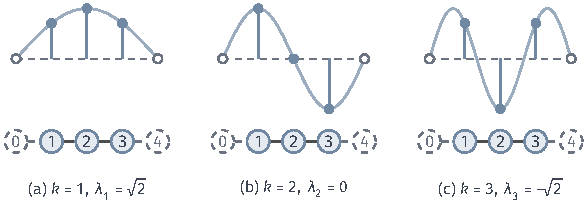
\includegraphics{figures/03-graphs/05-matrices-and-spectra/tikz/adjacency-path-sine-modes/figure.pdf}
  \caption{三点路径$P_3$上的三个正弦特征模式。底部虚线圆圈$0$和$4$为取零值的虚拟边界点，实线圆圈$1,2,3$为路径的实际顶点；上方曲线为$\sin(k\pi t/4)$，蓝色竖杆标出各顶点处的特征向量分量。(a) 基模$k=1$，$\lambda_1=\sqrt{2}$。(b) 二阶模$k=2$，$\lambda_2=0$。(c) 三阶模$k=3$，$\lambda_3=-\sqrt{2}$。}
  \label{fig:adjacency-path-sine-modes}
\end{BookInlineFigure}

\subsection{笛卡儿积图}
\label{sec:adjacency-cartesian-product-spectrum}

许多高维网格和超立方体图都可以由低维简单图通过笛卡儿积拼接而成。设$\mathcal G=(V_{\mathcal G},E_{\mathcal G})$和$\mathcal H=(V_{\mathcal H},E_{\mathcal H})$是两张图，它们的\term{笛卡儿积图}（Cartesian product of graphs）记为$\mathcal G\square\mathcal H$：其顶点集为笛卡儿积$V_{\mathcal G}\times V_{\mathcal H}=\{(u,v):u\in V_{\mathcal G},v\in V_{\mathcal H}\}$，两个顶点对$(u,v)$与$(u',v')$之间有边相连，当且仅当每次恰好沿着一个因子图走一步、另一个坐标保持不变：
\begin{itemize}
\item 要么第二坐标相同（$v=v'$），且第一坐标在$\mathcal G$中相邻（$\{u,u'\}\in E_{\mathcal G}$）；
\item 要么第一坐标相同（$u=u'$），且第二坐标在$\mathcal H$中相邻（$\{v,v'\}\in E_{\mathcal H}$）。
\end{itemize}

图~\ref{fig:adjacency-cartesian-edge-directions}展示了两个单边图$K_2$（顶点为$\{0,1\}$）的笛卡儿积$K_2\square K_2$：四个顶点对$(0,0),(1,0),(1,1),(0,1)$中，蓝色横边只改变第一坐标$u$，绿色竖边只改变第二坐标$v$，对角顶点$(0,0)$与$(1,1)$因同时改变了两个坐标而不相邻，最终围成四元环$C_4$。

\begin{BookInlineFigure}
  \centering
  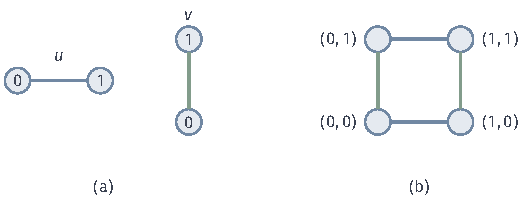
\includegraphics{figures/03-graphs/05-matrices-and-spectra/tikz/adjacency-cartesian-edge-directions/figure.pdf}
  \caption{两个单边图$K_2$的笛卡儿积$K_2\square K_2=C_4$。(a) 两个因子图分别提供第一坐标$u$与第二坐标$v$上的单步移动。(b) 蓝色横边只改变第一坐标$u$，绿色竖边只改变第二坐标$v$，四个顶点对围成四元环。}
  \label{fig:adjacency-cartesian-edge-directions}
\end{BookInlineFigure}

设$\mathcal G$有$p$个顶点、邻接矩阵为$\bm A_{\mathcal G}\in\mathbb R^{p\times p}$，$\mathcal H$有$q$个顶点、邻接矩阵为$\bm A_{\mathcal H}\in\mathbb R^{q\times q}$。按字典序排列$\mathcal G\square\mathcal H$的$pq$个顶点对：第一类边（改变$u$、保持$v$不变）对应的邻接作用是Kronecker积$\bm A_{\mathcal G}\otimes\bm I_q$；第二类边（保持$u$不变、改变$v$）对应的邻接作用是$\bm I_p\otimes\bm A_{\mathcal H}$。两类邻居相加，得到笛卡儿积图的邻接矩阵公式：
\begin{equation}
\bm A_{\mathcal G\square\mathcal H}
=\bm A_{\mathcal G}\otimes\bm I_q+\bm I_p\otimes\bm A_{\mathcal H}.
\label{eq:adjacency-cartesian-product}
\end{equation}

现在设$\bm x\in\mathbb R^p$是$\bm A_{\mathcal G}$属于特征值$\lambda$的特征向量（$\bm A_{\mathcal G}\bm x=\lambda\bm x$），$\bm y\in\mathbb R^q$是$\bm A_{\mathcal H}$属于特征值$\mu$的特征向量（$\bm A_{\mathcal H}\bm y=\mu\bm y$）。考察张量积向量$\bm x\otimes\bm y\in\mathbb R^{pq}$（它在顶点对$(u,v)$处的分量为乘积$x_u y_v$）。利用Kronecker积的混合乘积性质$(\bm M_1\otimes\bm M_2)(\bm x\otimes\bm y)=(\bm M_1\bm x)\otimes(\bm M_2\bm y)$，将$\bm A_{\mathcal G\square\mathcal H}$作用在$\bm x\otimes\bm y$上：
\[
\begin{aligned}
\bm A_{\mathcal G\square\mathcal H}(\bm x\otimes\bm y)
&=(\bm A_{\mathcal G}\bm x)\otimes(\bm I_q\bm y)+(\bm I_p\bm x)\otimes(\bm A_{\mathcal H}\bm y)\\
&=(\lambda\bm x)\otimes\bm y+\bm x\otimes(\mu\bm y)
=(\lambda+\mu)(\bm x\otimes\bm y).
\end{aligned}
\]
这表明$\bm x\otimes\bm y$是$\bm A_{\mathcal G\square\mathcal H}$的特征向量，对应的特征值恰好是两个因子特征值之和$\lambda+\mu$。分别取$\bm A_{\mathcal G}$的$p$个正交特征向量和$\bm A_{\mathcal H}$的$q$个正交特征向量，两两作Kronecker积共得到$pq$个两两正交的特征向量，张成整个$\mathbb R^{pq}$。

\begin{theorem}[笛卡儿积图的邻接谱]
\label{thm:adjacency-cartesian-product-spectrum}
设图$\mathcal G$的全部邻接特征值为$\lambda_1,\ldots,\lambda_p$（对应正交特征基$\bm x_1,\ldots,\bm x_p$），图$\mathcal H$的全部邻接特征值为$\mu_1,\ldots,\mu_q$（对应正交特征基$\bm y_1,\ldots,\bm y_q$）。则笛卡儿积图$\mathcal G\square\mathcal H$的全部$pq$个邻接特征值为两两之和
\[
\bigl\{\lambda_i+\mu_j:1\le i\le p,\;1\le j\le q\bigr\},
\]
其中$\lambda_i+\mu_j$对应的特征向量为$\bm x_i\otimes\bm y_j$。
\end{theorem}

定理~\ref{thm:adjacency-cartesian-product-spectrum}的一个经典应用是计算$d$维超立方体图$Q_d$的谱。$Q_d$的$2^d$个顶点是长度为$d$的$0$--$1$比特串$\{0,1\}^d$，两个比特串相邻当且仅当它们恰好在一个比特位上不同——这正是$d$个单边图$K_2$的连乘笛卡儿积$Q_d=K_2\square K_2\square\cdots\square K_2$。单边图$K_2$的两个特征值为$+1$和$-1$。在$d$个因子中各选一个特征值相加，若有$j$个因子选了$-1$、其余$d-j$个因子选了$+1$，则特征值之和为$(d-j)\cdot 1+j\cdot(-1)=d-2j$。从$d$个因子中挑出$j$个取$-1$共有$\binom{d}{j}$种选法，因此$Q_d$的特征值为$d-2j$（$j=0,1,\ldots,d$），重数为$\binom{d}{j}$。例如三维立方体$Q_3$的$8$个特征值为$3,1,1,1,-1,-1,-1,-3$。

\subsection{正则图的补图}
\label{sec:adjacency-complement-spectrum}

\begin{definition}[正则图]
\label{def:regular-graph}
若简单无向图$\mathcal G$的每个顶点都恰好有$d$个邻居（即所有顶点的度均等于$d$），则称$\mathcal G$为\term{$d$正则图}（$d$-regular graph）。
\end{definition}

在$d$正则图中，邻接矩阵$\bm A$的每一行都有$d$个$1$，行和恒等于$d$。因此给所有顶点统一赋读数$1$时，每个顶点的邻居读数之和都是$d$，即
\[
\bm A\bm 1=d\bm 1.
\]
这说明常向量$\bm 1$必定是$d$正则图属于特征值$d$的特征向量。又因$\bm A$是实对称矩阵，与常向量正交的零和子空间$\bm 1^\perp=\{\bm x\in\mathbb R^n:\bm 1^\top\bm x=0\}$在$\bm A$的作用下保持不变：对任意$\bm x\in\bm 1^\perp$，有$\bm 1^\top(\bm A\bm x)=(\bm A\bm 1)^\top\bm x=d(\bm 1^\top\bm x)=0$。于是我们可以在$\bm 1^\perp$内选出其余$n-1$个正交特征向量$\bm u_2,\ldots,\bm u_n$，这一性质使正则图的补图谱可以直接由原图谱换算出来。

\begin{theorem}[正则图的补图谱]
\label{thm:adjacency-regular-complement}
设$\mathcal G$是$n$个顶点的$d$正则简单无向图，其邻接特征值为$d=\lambda_1\ge\lambda_2\ge\cdots\ge\lambda_n$（其中$\lambda_1=d$对应常向量$\bm 1$，其余$\lambda_2,\ldots,\lambda_n$对应$\bm 1^\perp$中的正交特征向量$\bm u_2,\ldots,\bm u_n$）。则其补图$\overline{\mathcal G}$是$(n-1-d)$正则图，且$\overline{\mathcal G}$的全部邻接特征值为
\[
n-1-d\quad(\text{对应 }\bm 1),
\qquad\text{以及}\qquad
-1-\lambda_i\quad(i=2,\ldots,n,\text{ 对应 }\bm u_i).
\]
\end{theorem}

\begin{proof}
补图$\overline{\mathcal G}$保留相同的顶点集$V$，在所有互异且在原图$\mathcal G$中不相邻的顶点对之间连边。完全图的邻接矩阵为$\bm J-\bm I$，从中减去原图的邻接矩阵$\bm A_{\mathcal G}$，就得到补图的邻接矩阵：
\begin{equation}
\bm A_{\overline{\mathcal G}}=\bm J-\bm I-\bm A_{\mathcal G}.
\label{eq:adjacency-complement-matrix}
\end{equation}

分别考察$\bm A_{\overline{\mathcal G}}$在常向量$\bm 1$和在$\bm u_i\in\bm 1^\perp$（$i=2,\ldots,n$）上的作用：
\begin{itemize}
\item 在常向量$\bm 1$上，$\bm J\bm 1=n\bm 1$且$\bm A_{\mathcal G}\bm 1=d\bm 1$，故
\[
\bm A_{\overline{\mathcal G}}\bm 1=(\bm J-\bm I-\bm A_{\mathcal G})\bm 1=(n-1-d)\bm 1;
\]
\item 对每个$i\in\{2,\ldots,n\}$，因为$\bm u_i\in\bm 1^\perp$，有$\bm J\bm u_i=\bm 1(\bm 1^\top\bm u_i)=\bm 0$，且$\bm A_{\mathcal G}\bm u_i=\lambda_i\bm u_i$，故
\[
\bm A_{\overline{\mathcal G}}\bm u_i=(\bm J-\bm I-\bm A_{\mathcal G})\bm u_i=\bm 0-\bm u_i-\lambda_i\bm u_i=(-1-\lambda_i)\bm u_i.
\]
\end{itemize}
这$n$个正交特征向量给出了$\overline{\mathcal G}$的全部$n$个特征值。注意当原图$\mathcal G$不连通时，部分$i\geq 2$也可能满足$\lambda_i=d$，但由于$\bm u_i\in\bm 1^\perp$，它们在补图中均按$-1-\lambda_i=-1-d$换算。
\end{proof}

以四元环$C_4$（$n=4,d=2$）检验定理~\ref{thm:adjacency-regular-complement}：$C_4$的谱为$\lambda_1=2,\lambda_2=0,\lambda_3=0,\lambda_4=-2$。其补图$\overline{C_4}$只保留两条互不相交的对角边$\{1,3\}$与$\{2,4\}$（即$K_2\sqcup K_2$）。代入换算公式：常向量方向给出$n-1-d=4-1-2=1$；$\bm 1^\perp$中的三个特征值$0,0,-2$依次变为$-1-0=-1$、$-1-0=-1$、$-1-(-2)=1$。补图谱为$\{1,1,-1,-1\}$，与两条独立边各贡献一对$\pm1$完全一致。反之，若原图不是正则图，则$\bm A_{\mathcal G}\bm 1$的各分量是互不相等的顶点度，常向量$\bm 1$不再是$\bm A_{\mathcal G}$的特征向量，$\bm A_{\mathcal G}$与$\bm J$无法在常向量与$\bm 1^\perp$上同时对角化，上述简单换算公式便不再适用。

\section{谱的性质}
\label{sec:adjacency-spectral-properties}

上一节通过直接构造特征向量求出了几类典型图的完整谱。现在回到一般的图，研究邻接谱本身具有哪些普遍的结构性质。我们依次回答四个核心问题：
\begin{enumerate}
\item 最大特征值$\lambda_1$为什么地位特殊？它的重数是多少，对应的特征向量有什么符号特征？
\item 不必解出全部特征值，能否直接用顶点的度给出$\lambda_1$的上下界？
\item 从图中删去边、减小边权或删去顶点后，$\lambda_1$会如何变化？
\item 什么时候正特征值$\lambda$与负特征值$-\lambda$必定成对出现？
\end{enumerate}

本节在非负加权图的一般框架下统一讨论这些问题：设$\bm W=(w_{i,j})\in\mathbb R^{n\times n}$为非负实对称加权邻接矩阵（对角元$w_{i,i}=0$，边权$w_{i,j}=w_{j,i}\geq 0$）；简单无权图的邻接矩阵$\bm A$正是每条边权取$1$的特例。顶点$i$的加权度定义为第$i$行的边权之和$d_i=\sum_{j=1}^n w_{i,j}$。

\subsection{连通图的Perron定理}
\label{sec:adjacency-perron-theorem}

对实对称矩阵$\bm W$，其最大特征值$\lambda_1$可以通过单位球面上的Rayleigh商极值（可参考\BookChapterRef{chap:matrix-approximation}{卷二"矩阵逼近"章}）刻画为
\[
\lambda_1=\max_{\|\bm x\|_2=1}\bm x^\top\bm W\bm x.
\]
为了看清怎样的单位向量$\bm x=(x_1,\ldots,x_n)^\top$能让二次型$\bm x^\top\bm W\bm x$尽可能大，我们把矩阵二次型按图的边展开：
\[
\bm x^\top\bm W\bm x
=\sum_{i=1}^n\sum_{j=1}^n w_{i,j}x_i x_j
=2\sum_{\{i,j\}\in E}w_{i,j}x_i x_j.
\]
这里每一条无向边$\{i,j\}\in E$在双重大和中作为有序对$(i,j)$和$(j,i)$各出现一次，合并贡献$2w_{i,j}x_i x_j$。

观察单条正权边$\{i,j\}$（$w_{i,j}>0$）上的乘积项$2w_{i,j}x_i x_j$：如果两端顶点的赋值$x_i$与$x_j$正负号相反（例如一端取$+1$、另一端取$-1$），乘积$x_i x_j<0$，这条边就会给二次型带来负贡献$-2w_{i,j}|x_i||x_j|$，把总和往小里拉；反之，如果我们把向量$\bm x$的每一个分量都取绝对值，构造非负向量
\[
|\bm x|=\bigl(|x_1|,|x_2|,\ldots,|x_n|\bigr)^\top,
\]
那么一方面向量的欧氏长度完全不变：
\[
\bigl\||\bm x|\bigr\|_2=\sqrt{\sum_{i=1}^n |x_i|^2}=\sqrt{\sum_{i=1}^n x_i^2}=\|\bm x\|_2;
\]
另一方面，由于边权$w_{i,j}\geq 0$，每条边上的乘积都满足$w_{i,j}|x_i||x_j|\geq w_{i,j}x_i x_j$，因此二次型总和只会增大或保持不变：
\[
|\bm x|^\top\bm W|\bm x|
=2\sum_{\{i,j\}\in E}w_{i,j}|x_i||x_j|
\geq 2\sum_{\{i,j\}\in E}w_{i,j}x_i x_j
=\bm x^\top\bm W\bm x.
\]
这意味着：在单位球面上寻找最大化二次型的特征方向时，总可以选到各分量全非负的向量。

图~\ref{fig:adjacency-perron-absolute-value}在三点路径$1\!-\!2\!-\!3$（含两条单位权边$\{1,2\}$和$\{2,3\}$）上直观对比了取绝对值前后的效果。在图~\ref{fig:adjacency-perron-absolute-value}(a)中，取正负交替赋值$\bm x=(1,-1,1)^\top$，两条边的端点乘积均为$x_1x_2=x_2x_3=-1$，二次型为$\bm x^\top\bm A\bm x=2(-1)+2(-1)=-4$，Rayleigh商为$-4/3$；在图~\ref{fig:adjacency-perron-absolute-value}(b)中，逐分量取绝对值得到$|\bm x|=(1,1,1)^\top$，向量长度仍为$\sqrt{3}$，但两条边的端点乘积均变为$+1$，二次型跃升为$|\bm x|^\top\bm A|\bm x|=2(+1)+2(+1)=+4$，Rayleigh商提高到$+4/3$。

\begin{BookInlineFigure}
  \centering
  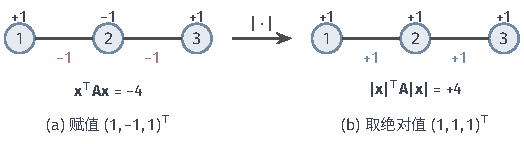
\includegraphics{figures/03-graphs/05-matrices-and-spectra/tikz/adjacency-perron-absolute-value/figure.pdf}
  \caption{三点路径$1\!-\!2\!-\!3$上逐分量取绝对值前后的二次型变化。边下方标注的是端点乘积$x_i x_j$。(a) 赋值$\bm x=(1,-1,1)^\top$时，两条边两端均异号，端点乘积为$-1$，二次型$\bm x^\top\bm A\bm x=2(-1-1)=-4$。(b) 取绝对值得到$|\bm x|=(1,1,1)^\top$后，向量长度不变，每条边的端点乘积变为$+1$，二次型升至$+4$。}
  \label{fig:adjacency-perron-absolute-value}
\end{BookInlineFigure}

在进入正式定理之前，我们先明确加权矩阵$\bm W$的连通条件。在矩阵乘向量$(\bm W\bm x)_i=\sum_{j=1}^n w_{i,j}x_j$中，若两个顶点$i,j$之间的权重$w_{i,j}=0$，则$x_j$对第$i$个输出分量没有任何贡献，二者在矩阵作用中互不相连；只有满足$w_{i,j}>0$的正权边才真正传递数值。为此给出正权支撑的正式定义。

\begin{definition}[正权支撑]
\label{def:positive-weight-support}
设$\bm W=(w_{i,j})\in\mathbb R^{n\times n}$为顶点集$V$上的非负对称邻接权矩阵（对角元$w_{i,i}=0$，边权$w_{i,j}=w_{j,i}\geq 0$）。保留全体顶点$V$、仅保留严格正权边
\begin{equation}
E_+=\bigl\{\{i,j\}\subseteq V:w_{i,j}>0\bigr\}
\label{eq:positive-weight-support}
\end{equation}
所构成的无权简单图$\mathcal G_+=(V,E_+)$称为加权图（或矩阵$\bm W$）的\term{正权支撑}（positive-weight support）。
\end{definition}

当正权支撑$\mathcal G_+$连通时，任意两个顶点之间都存在一条每步边权均严格大于零的路径，非零读数才能沿正权路径传遍全图所有顶点。

\begin{theorem}[连通图的Perron定理]
\label{thm:adjacency-perron}
设$\bm W=(w_{i,j})\in\mathbb R^{n\times n}$为有限无向图的非负对称邻接权矩阵，且其正权支撑$\mathcal G_+$连通（$n\geq 2$）。则：
\begin{enumerate}
\item 最大特征值$\lambda_1>0$的代数重数为$1$，且存在各分量均严格为正的特征向量$\bm p=(p_1,\ldots,p_n)^\top$（$p_i>0,\forall i$）；
\item $\bm W$的任意特征值$\lambda$均满足$|\lambda|\leq\lambda_1$（即谱半径等于$\lambda_1$）。
\end{enumerate}
\end{theorem}

\begin{proof}
我们分三步依次证明：（1）存在各分量严格为正的最大特征向量$\bm p$；（2）最大特征值$\lambda_1$的特征空间是一维的（重数为$1$）；（3）其余特征值均满足$|\lambda|\leq\lambda_1$。

\textbf{第一步（严格正特征向量的存在性）}：在单位球面$\|\bm x\|_2=1$上任取一个使Rayleigh商达到最大值$\lambda_1$的单位特征向量$\bm x$，令$\bm p=|\bm x|$。由前面的绝对值不等式，有
\[
\lambda_1\geq\bm p^\top\bm W\bm p
=\sum_{i,j}w_{i,j}|x_i||x_j|
\geq\sum_{i,j}w_{i,j}x_i x_j
=\bm x^\top\bm W\bm x=\lambda_1,
\]
且$\|\bm p\|_2=\|\bm x\|_2=1$。因此$\bm p^\top\bm W\bm p=\lambda_1$，即非负单位向量$\bm p$也在单位球面上达到最大Rayleigh商$\lambda_1$。由Rayleigh商在极值点处的驻点条件，$\bm p$本身就是属于最大特征值$\lambda_1$的特征向量：$\bm W\bm p=\lambda_1\bm p$。又因正权支撑连通且$n\geq 2$，图中至少有一条正权边，取常向量即可见$\lambda_1>0$。

下面用反证法说明$\bm p$不可能含有零分量。假设存在某个顶点$i$使得$p_i=0$。读取特征方程$\bm W\bm p=\lambda_1\bm p$的第$i$行：
\[
0=\lambda_1 p_i=\sum_{j=1}^n w_{i,j}p_j.
\]
由于右端每一项都满足$w_{i,j}\geq 0$且$p_j\geq 0$，非负项之和等于零迫使每一项都等于零。特别地，对顶点$i$在正权支撑中的每一个邻居$j$（满足$w_{i,j}>0$），都必有$p_j=0$。也就是说，“分量为零”这一性质会从顶点$i$传播到它的所有正权邻居。由于正权支撑$\mathcal G_+$连通，从$i$出发沿正权路径逐歩传递，最终推出全图所有顶点的分量都满足$p_k=0$（$\forall k\in V$），即$\bm p=\bm 0$，这与$\|\bm p\|_2=1$矛盾。因此$\bm p$的每个分量都严格为正：$p_i>0$（$\forall i\in V$）。

\textbf{第二步（$\lambda_1$的重数为$1$）}：用反证法。假设$\lambda_1$的特征子空间维数大于$1$，则可以在该特征子空间中选出一个与$\bm p$正交的单位特征向量$\bm y$（满足$\bm W\bm y=\lambda_1\bm y$，$\|\bm y\|_2=1$，且$\langle\bm p,\bm y\rangle=0$）。

对$\bm y$重复第一步的推导：令$|\bm y|=(|y_1|,\ldots,|y_n|)^\top$，则$|\bm y|$也是属于$\lambda_1$的非负单位特征向量；再由第一步的零分量传播论证，可知$|\bm y|$的每个分量都严格为正，从而$\bm y$的每个分量都非零（$y_i\neq 0,\forall i\in V$）。

另一方面，由于$|\bm y|^\top\bm W|\bm y|=\bm y^\top\bm W\bm y=\lambda_1$，不等式
\[
\sum_{\{i,j\}\in E}2w_{i,j}|y_i||y_j|
\geq\sum_{\{i,j\}\in E}2w_{i,j}y_i y_j
\]
必须取等号。因为每一条边上的差$2w_{i,j}(|y_i||y_j|-y_i y_j)\geq 0$都非负，总和为零要求每一条正权边$\{i,j\}\in E_+$（$w_{i,j}>0$）都满足$|y_i||y_j|=y_i y_j$。由于$y_i\neq 0$且$y_j\neq 0$，这意味着正权边的两个端点$y_i$与$y_j$必须严格同号。沿连通的正权支撑传递，向量$\bm y$的所有$n$个分量必定同为正数或同为负数。然而$\bm p$的所有分量严格为正，于是内积$\langle\bm p,\bm y\rangle=\sum_{i=1}^n p_i y_i$是$n$个严格同号非零项之和，绝不可能等于$0$——这与$\langle\bm p,\bm y\rangle=0$矛盾。故$\lambda_1$的特征空间只能是一维的，重数为$1$。

\textbf{第三步（谱半径界$|\lambda|\leq\lambda_1$）}：任取$\bm W$的一个特征值$\lambda$及其单位特征向量$\bm z$（$\|\bm z\|_2=1$）。由三角不等式与$\lambda_1$的极大性质，
\[
|\lambda|
=|\bm z^\top\bm W\bm z|
=\Bigl|\sum_{i,j}w_{i,j}z_i z_j\Bigr|
\leq\sum_{i,j}w_{i,j}|z_i||z_j|
=|\bm z|^\top\bm W|\bm z|
\leq\lambda_1,
\]
定理证毕。
\end{proof}

定理~\ref{thm:adjacency-perron}中唯一确定的严格正单位特征向量$\bm p$称为图的\term{Perron向量}（Perron vector）。需要注意，定理保证最大特征值$\lambda_1$本身是单根，但并不排除最小特征值$\lambda_n$达到相反数$-\lambda_1$（此时$|\lambda_n|=\lambda_1$）。例如单边图$K_2$的特征值为$+1$和$-1$。第~\ref{sec:adjacency-bipartite-symmetry}小节将证明：在正权支撑连通图上，$\lambda_n=-\lambda_1$发生当且仅当该图是二部图。

\subsection{谱的上下界}
\label{sec:adjacency-degree-bounds}

Perron定理确立了最大特征值$\lambda_1$的单根性与正特征向量，但在一般非正则图上并不能直接写出$\lambda_1$的闭式解。下面我们分别利用Rayleigh商的下界性质和Perron向量的最大分量，证明$\lambda_1$始终被夹在图的平均度$\overline d$与最大度$d_{\max}$之间。

\paragraph{下界：用全一常向量测试Rayleigh商}

根据Rayleigh商的极大性质，最大特征值$\lambda_1$是$\frac{\bm x^\top\bm W\bm x}{\bm x^\top\bm x}$在所有非零向量$\bm x\neq\bm 0$上的最大值：
\[
\lambda_1=\max_{\bm x\neq\bm 0}\frac{\bm x^\top\bm W\bm x}{\bm x^\top\bm x}.
\]
因此，我们随便挑选一个具体的非零向量$\bm x$代进去算出的Rayleigh商，都必然小于或等于最大值$\lambda_1$。

取最简单的全一常向量$\bm x=\bm 1=(1,1,\ldots,1)^\top\in\mathbb R^n$（所有顶点赋相同的读数$1$），分两步计算它的Rayleigh商。先算矩阵乘向量$\bm W\bm 1$：按矩阵乘法规则，$\bm W\bm 1$的第$i$个分量是把$\bm W$第$i$行的所有元素各自乘以$1$再相加：
\[
(\bm W\bm 1)_i=\sum_{j=1}^n w_{i,j}\cdot 1=\sum_{j=1}^n w_{i,j}=d_i.
\]
也就是说，对全一向量$\bm 1$作用一次邻接矩阵$\bm W$，输出向量的第$i$个分量恰好就是顶点$i$的加权度$d_i$，即$\bm W\bm 1=(d_1,d_2,\ldots,d_n)^\top$（若改用单位化常向量$\bm u=\frac{1}{\sqrt n}\bm 1$，则输出的第$i$个分量为$d_i/\sqrt n$）。

再算二次型与Rayleigh商：用行向量$\bm 1^\top$左乘输出向量$\bm W\bm 1$，相当于把全部$n$个顶点的度相加：
\[
\bm 1^\top\bm W\bm 1=\sum_{i=1}^n 1\cdot(\bm W\bm 1)_i=\sum_{i=1}^n d_i.
\]
而全一向量本身的长度平方为$\bm 1^\top\bm 1=\sum_{i=1}^n 1^2=n$。将两者相除，就得到全一向量$\bm 1$的Rayleigh商恰好等于全图的平均度$\overline d$：
\[
\frac{\bm 1^\top\bm W\bm 1}{\bm 1^\top\bm 1}
=\frac{1}{n}\sum_{i=1}^n d_i
=\overline d.
\]
在简单无权图中，每条无向边为两个端点的度各贡献$1$，总度数$\sum_{i=1}^n d_i=2m$，故平均度为$\overline d=2m/n$。由于最大值$\lambda_1$不小于特定向量$\bm 1$的Rayleigh商，立即得到下界：
\[
\lambda_1\geq\overline d.
\]

\paragraph{上界：在Perron向量的最大分量处放缩}

再证上界$\lambda_1\leq d_{\max}$，其中$d_{\max}=\max_{1\leq i\leq n}d_i$为全图的最大度。取属于$\lambda_1$的非负特征向量$\bm p=(p_1,\ldots,p_n)^\top\neq\bm 0$（连通图上即为严格正的Perron向量），并在全部$n$个顶点中找出分量最大的那个顶点$i^\star$，使得
\[
p_{i^\star}=\max_{1\leq j\leq n}p_j>0.
\]
写出特征方程$\bm W\bm p=\lambda_1\bm p$在顶点$i^\star$这一行的等式，并将右端每个邻居的分量$p_j$放大为最大值$p_{i^\star}$（注意到$w_{i^\star,j}\geq 0$）：
\[
\lambda_1 p_{i^\star}
=\sum_{j=1}^n w_{i^\star,j}\,p_j
\leq\sum_{j=1}^n w_{i^\star,j}\,p_{i^\star}
=\Bigl(\sum_{j=1}^n w_{i^\star,j}\Bigr)p_{i^\star}
=d_{i^\star}\,p_{i^\star}
\leq d_{\max}\,p_{i^\star}.
\]
因为$p_{i^\star}>0$，在不等式两端同除以正数$p_{i^\star}$，即得上界$\lambda_1\leq d_{\max}$。

\begin{theorem}[最大邻接特征值的度界]
\label{prop:adjacency-degree-bounds}
对任意非负实对称邻接矩阵$\bm W\in\mathbb R^{n\times n}$，其最大特征值$\lambda_1$满足
\begin{equation}
\overline d\leq\lambda_1\leq d_{\max}.
\label{eq:adjacency-degree-spectral-bounds}
\end{equation}
若$\bm W$的正权支撑连通，则$\lambda_1=\overline d$（或$\lambda_1=d_{\max}$）成立当且仅当图中所有顶点的加权度均相等（即图为正则图）。
\end{theorem}

\paragraph{取等条件}

我们来追踪正权支撑连通时式~\eqref{eq:adjacency-degree-spectral-bounds}两端何时取等号。若上界$\lambda_1=d_{\max}$取等，则前面关于最大分量顶点$i^\star$的两步放缩必须同时取等号：第一步等号$\sum_j w_{i^\star,j}(p_{i^\star}-p_j)=0$要求$i^\star$的每一个正权邻居$j$（$w_{i^\star,j}>0$）都达到最大分量$p_j=p_{i^\star}$，第二步等号要求$d_{i^\star}=d_{\max}$。既然正权邻居$j$也达到了最大分量$p_j=p_{i^\star}$，对顶点$j$再次应用同样的推理，可知$d_j=d_{\max}$且$j$的所有正权邻居分量也等于$p_{i^\star}$。沿连通的正权支撑传遍全图，所有顶点的度都必须等于$d_{\max}$，图必为正则图。

若下界$\lambda_1=\overline d$取等，则说明常向量$\bm 1$的Rayleigh商已经达到了全局最大值$\lambda_1$，因此$\bm 1$本身就是属于$\lambda_1$的特征向量，满足$\bm W\bm 1=\overline d\,\bm 1$。逐分量读取该式，即得对所有顶点$i$都有$d_i=(\bm W\bm 1)_i=\overline d$，图同样是正则图。

以三点路径$P_3$和四点环$C_4$对照：$P_3$的度序列为$(1,2,1)$，平均度$\overline d=4/3\approx 1.333$，最大特征值$\lambda_1=\sqrt 2\approx 1.414$，最大度$d_{\max}=2$，满足严格不等式$4/3<\sqrt 2<2$；而$2$正则图$C_4$的度序列为$(2,2,2,2)$，三者相等$\overline d=\lambda_1=d_{\max}=2$。

\subsection{子图的谱单调性}
\label{sec:adjacency-spectral-monotonicity}

如果在图中删去一条边、降低某条边的正权重，或者删去一个顶点及其关联边，每个顶点的邻居贡献只减不增。下面用非负最大化向量证明：最大特征值$\lambda_1$对子图具有单调性，且在连通图上删去任何正权边或顶点都会使$\lambda_1$严格下降。

设$\bm W'\in\mathbb R^{n\times n}$是由$\bm W\in\mathbb R^{n\times n}$减小部分边权（包括将边权降为$0$以表示删边，或将某个被删顶点的整行整列置为$0$）所得的非负对称矩阵，满足逐元素$0\leq w'_{i,j}\leq w_{i,j}$。在$\bm W'$上取一个非负单位特征向量$\bm x\geq\bm 0$（$\|\bm x\|_2=1$）使得$\bm x^\top\bm W'\bm x=\lambda_1(\bm W')$。将同一个非负单位向量$\bm x$代入原矩阵$\bm W$的二次型比较：
\[
\lambda_1(\bm W')
=\bm x^\top\bm W'\bm x
=\sum_{i,j}w'_{i,j}x_i x_j
\leq\sum_{i,j}w_{i,j}x_i x_j
=\bm x^\top\bm W\bm x
\leq\lambda_1(\bm W).
\]
这里第一个不等式来自$0\leq w'_{i,j}\leq w_{i,j}$与$x_i x_j\geq 0$，第二个不等式来自$\lambda_1(\bm W)$是$\bm W$在单位球面上的最大Rayleigh商。

进一步，若原图$\bm W$的正权支撑连通，且$\bm W'\neq\bm W$（确实减小了至少一条边$\{u,v\}$的权重$w'_{u,v}<w_{u,v}$），能否出现等号$\lambda_1(\bm W')=\lambda_1(\bm W)$？若两端相等，则上面不等式链中的两处不等号都必须取等：一方面，第二处取等$\bm x^\top\bm W\bm x=\lambda_1(\bm W)$说明$\bm x$也是连通矩阵$\bm W$达到$\lambda_1(\bm W)$的单位特征向量，由定理~\ref{thm:adjacency-perron}（Perron定理）知$\bm x$的每一个分量都严格为正（$x_i>0,\forall i\in V$）；另一方面，既然$x_u>0$且$x_v>0$，在权重严格减小的那条边$\{u,v\}$上就有$w'_{u,v}x_u x_v<w_{u,v}x_u x_v$，导致第一处不等式严格成立$\bm x^\top\bm W'\bm x<\bm x^\top\bm W\bm x$，产生矛盾。因此，在正权支撑连通图上，删去任意正权边、降低任意正权边的权重，或删去任意顶点，都会使最大邻接特征值严格减小：$\lambda_1(\bm W')<\lambda_1(\bm W)$。

例如从$n$点环$C_n$中删去一条边得到路径$P_n$，最大特征值从$\lambda_1(C_n)=2$严格下降为$\lambda_1(P_n)=2\cos\bigl(\frac{\pi}{n+1}\bigr)<2$。反之，若原图不连通，例如取$\mathcal G=C_4\sqcup K_2$，其最大特征值$\lambda_1=2$由$C_4$分量单独决定；此时删去较小分量$K_2$中的边并不会改变全图的最大特征值$\lambda_1=2$，这说明严格单调性确实依赖原图的连通性假设。

\subsection{二部图的谱对称性}
\label{sec:adjacency-bipartite-symmetry}

前面三小节聚焦于谱右端的最大特征值$\lambda_1$。现在我们把目光转向整个邻接谱的左右两端：在什么条件下，图的邻接谱关于原点对称（即每个特征值$\lambda$与$-\lambda$以相同重数成对出现）？答案恰好刻画了二部图。

先看二部图为什么必然具有对称谱。设图$\mathcal G$是二部图，其顶点集划分为左右两个独立集$V=X\cup Y$，所有正权边都横跨在$X$与$Y$之间（同侧内部没有任何正权边）。我们构造一个$n\times n$对角符号矩阵$\bm S=\operatorname{diag}(s_1,\ldots,s_n)$：
\[
s_i=
\begin{cases}
+1,& i\in X,\\
-1,& i\in Y.
\end{cases}
\]
显然$\bm S^\top=\bm S$且$\bm S^2=\bm I$（$\bm S$是正交对合矩阵）。考察正交相似变换$\bm S\bm W\bm S$的第$(i,j)$个元素$s_i w_{i,j}s_j$：当$w_{i,j}>0$时，边$\{i,j\}$连接$X$与$Y$异侧端点，必有$s_i s_j=(+1)(-1)=-1$，故$s_i w_{i,j}s_j=-w_{i,j}$；当$w_{i,j}=0$时，同样有$s_i w_{i,j}s_j=0=-w_{i,j}$。因此，对角符号矩阵$\bm S$把整个邻接权矩阵$\bm W$变成了它的相反数：
\begin{equation}
\bm S\bm W\bm S=-\bm W,\qquad\text{或等价地}\qquad \bm W\bm S=-\bm S\bm W.
\label{eq:adjacency-bipartite-anticommute}
\end{equation}

利用式~\eqref{eq:adjacency-bipartite-anticommute}，若$\bm x$是$\bm W$属于特征值$\lambda$的特征向量（$\bm W\bm x=\lambda\bm x$），将$\bm W$作用在翻转了$Y$侧符号的向量$\bm S\bm x$上：
\[
\bm W(\bm S\bm x)=-\bm S\bm W\bm x=-\bm S(\lambda\bm x)=(-\lambda)(\bm S\bm x).
\]
这表明$\bm S\bm x$正是$\bm W$属于相反数特征值$-\lambda$的特征向量。图~\ref{fig:adjacency-bipartite-sign-flip}在四元环$C_4$（二部划分$X=\{1,3\},Y=\{2,4\}$）上展示了这一操作：将属于$\lambda=+2$的特征向量$\bm x=(1,1,1,1)^\top$在$Y$侧变号，立即得到属于$-\lambda=-2$的特征向量$\bm S\bm x=(1,-1,1,-1)^\top$。由于可逆矩阵$\bm S$在$\lambda$的特征子空间与$-\lambda$的特征子空间之间建立了线性同构，两个特征值$\lambda$与$-\lambda$的代数重数必然完全相等，即整个邻接谱关于原点对称：$\lambda_i=-\lambda_{n+1-i}$（$i=1,\ldots,n$）。

\begin{BookInlineFigure}
  \centering
  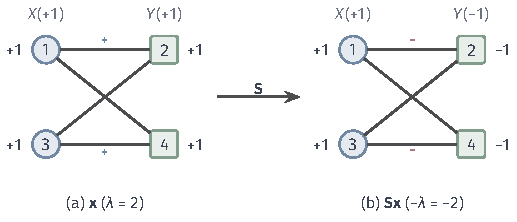
\includegraphics{figures/03-graphs/05-matrices-and-spectra/tikz/adjacency-bipartite-sign-flip/figure.pdf}
  \caption{二部图上的对角符号翻转$\bm S\bm W\bm S=-\bm W$（以$C_4$为例，圆点为$X=\{1,3\}$，方点为$Y=\{2,4\}$）。(a) 属于特征值$\lambda=+2$的特征向量$\bm x=(1,1,1,1)^\top$，跨部边两端同号。(b) 经$\bm S$保持$X$侧符号、翻转$Y$侧符号后，跨部边两端全部反号，得到属于特征值$-\lambda=-2$的特征向量$\bm S\bm x=(1,-1,1,-1)^\top$。}
  \label{fig:adjacency-bipartite-sign-flip}
\end{BookInlineFigure}

反过来，谱关于原点对称（甚至在连通图上仅最小特征值满足$\lambda_n=-\lambda_1$）也能反推出图是二部图。

\begin{theorem}[二部图的谱对称性]
\label{thm:adjacency-bipartite-spectral-symmetry}
设$\bm W\in\mathbb R^{n\times n}$为有限无向无自环图的非负对称邻接权矩阵。则以下命题成立：
\begin{enumerate}
\item $\bm W$的邻接谱关于零对称（即对每个$i=1,\ldots,n$都有$\lambda_i=-\lambda_{n+1-i}$），当且仅当其正权支撑$\mathcal G_+$是二部图（不含奇数长度的环）；
\item 若进一步$\bm W$的正权支撑连通且$n\geq 2$，则只需两端特征值满足$\lambda_n=-\lambda_1$，即可判定正权支撑$\mathcal G_+$是二部图。
\end{enumerate}
\end{theorem}

\begin{proof}
\textbf{第1条}：充分性（二部图$\implies$谱关于零对称）已由式~\eqref{eq:adjacency-bipartite-anticommute}给出。下面证明必要性（谱关于零对称$\implies$不含奇环）：若邻接谱关于零对称，则对任意正奇数$k=1,3,5,\ldots$，每一对相反特征值$\lambda$与$-\lambda$的奇数次幂滿足$(-\lambda)^k=-\lambda^k$，相加相互抵消（零特征值的幂本身为$0$），因此所有奇数阶谱矩恒等于零：
\[
\operatorname{tr}(\bm W^k)=\sum_{i=1}^n\lambda_i^k=0,\qquad k=1,3,5,\ldots.
\]
假设正权支撑$\mathcal G_+$中含有一个奇数长度$\ell$的简单环$v_1\to v_2\to\cdots\to v_\ell\to v_1$。沿该奇环绕行一圈是一条长度为$\ell$的闭行走，其沿途每一步的边权均严格为正，乘积$w_{v_1,v_2}w_{v_2,v_3}\cdots w_{v_\ell,v_1}>0$为$(\bm W^\ell)_{v_1,v_1}$贡献了一个严格正数。由于$\bm W$的所有元素非负，其余一切$\ell$步闭行走的权重乘积均非负，不可能抵消这一正贡献，从而$\operatorname{tr}(\bm W^\ell)>0$，与奇数阶迹为零矛盾。故正权支撑$\mathcal G_+$中不含奇环，必为二部图。

\textbf{第2条}：设正权支撑$\mathcal G_+$连通（$n\geq 2$，从而$\lambda_1>0$）且$\lambda_n=-\lambda_1$。取属于最小特征值$\lambda_n$的实单位特征向量$\bm x$（$\bm W\bm x=\lambda_n\bm x$，$\|\bm x\|_2=1$），则$\bm x^\top\bm W\bm x=\lambda_n=-\lambda_1$。考察绝对值向量$|\bm x|=(|x_1|,\ldots,|x_n|)^\top$的二次型：
\[
\begin{aligned}
\lambda_1
&\geq|\bm x|^\top\bm W|\bm x|
=\sum_{i,j}w_{i,j}|x_i||x_j|
\geq\Bigl|\sum_{i,j}w_{i,j}x_i x_j\Bigr|\\
&=|\bm x^\top\bm W\bm x|
=-\bm x^\top\bm W\bm x
=-\lambda_n=\lambda_1.
\end{aligned}
\]
首尾两端相等迫使中间不等式全部取等号。首先，$|\bm x|^\top\bm W|\bm x|=\lambda_1$说明非负单位向量$|\bm x|$达到了最大特征值$\lambda_1$；由定理~\ref{thm:adjacency-perron}（Perron定理），$|\bm x|$是严格正的Perron向量，故$|x_i|>0$（即$x_i\neq 0,\forall i\in V$）。其次，$\sum_{i,j}w_{i,j}|x_i||x_j|=\sum_{i,j}w_{i,j}(-x_i x_j)$等价于
\[
\sum_{\{i,j\}\in E_+}2w_{i,j}\bigl(|x_i||x_j|+x_i x_j\bigr)=0.
\]
由于对每条边都有$|x_i||x_j|+x_i x_j\geq 0$且正权边满足$w_{i,j}>0$，每一条正权边$\{i,j\}\in E_+$都必须满足
\[
x_i x_j=-|x_i||x_j|<0.
\]
这意味着：每条正权边的两个端点在向量$\bm x$中的分量符号必定一正一负。令
\[
X=\{i\in V:x_i>0\},\qquad Y=\{i\in V:x_i<0\},
\]
由于每个$x_i\neq 0$，$V=X\cup Y$构成顶点集的一个划分，且所有正权边都连接$X$中的顶点与$Y$中的顶点，$X$与$Y$内部均无正权边。因此正权支撑$\mathcal G_+$是二部图。
\end{proof}

对比两个例子：四元环$C_4$的谱为$\{2,0,0,-2\}$，关于零对称且$\lambda_4=-2=-\lambda_1$，是二部图；三角形$C_3$的谱为$\{2,-1,-1\}$，不关于零对称且$\lambda_3=-1\neq -\lambda_1$，含有奇环。同时要注意第2条中“正权支撑连通”这一前提不可省略：若取不连通图$\mathcal G=C_3\sqcup K_{3,3}$，其中$C_3$的谱为$\{2,-1,-1\}$、二部图分量$K_{3,3}$的谱为$\{3,0,0,0,0,-3\}$，合在一起全图最大特征值$\lambda_1=3$与最小特征值$\lambda_9=-3$依然满足$\lambda_9=-\lambda_1$，但整张图因包含三角形分量$C_3$而不是二部图（此时完整谱中由$C_3$贡献的$+2$没有对应的$-2$，按第1条的完整谱对称性仍能准确排除二部性）。

\section{图结构的谱刻画}
\label{sec:adjacency-spectral-structure}

如果只知道一张简单无向图$\mathcal G=(V,E)$的邻接谱$\lambda_1\ge\lambda_2\ge\cdots\ge\lambda_n$，我们能从中恢复出哪些图的结构参数，又能对哪些组合不变量给出上下界？

本节从局部到全局依次展开：第~\ref{sec:adjacency-low-spectral-moments}小节由二阶、三阶谱矩计数边和三角形，并结合顶点度从四阶谱矩计算四环数；第~\ref{sec:adjacency-diameter-bound}小节利用矩阵幂的线性无关性证明不同特征值的个数至少比图的直径多$1$；第~\ref{sec:adjacency-chromatic-bounds}小节结合导出子图的谱交错性质与单位根相位消去法，给出图色数$\chi(\mathcal G)$的谱上下界；第~\ref{sec:adjacency-hoffman-independence}小节通过中心化指示向量的Rayleigh商导出正则图最大独立集$\alpha(\mathcal G)$的Hoffman上界；最后，第~\ref{sec:adjacency-spectral-information}小节通过同谱非同构图反例，总结完整邻接谱的信息边界。

\subsection{局部结构}
\label{sec:adjacency-low-spectral-moments}

设简单无向图$\mathcal G=(V,E)$有$n=|V|$个顶点、$m=|E|$条边，顶点$v$的度记为$d_v$。由第~\ref{sec:adjacency-walk-counts}节的谱矩公式~\eqref{eq:adjacency-spectral-moments}，第$k$阶谱矩$\sum_{i=1}^n\lambda_i^k=\operatorname{tr}(\bm A^k)$等于全图长度为$k$的闭行走总数。当$k=1$时，简单无向图没有自环，一步闭行走条数为零，故一阶谱矩恒为$\operatorname{tr}(\bm A)=\sum_{i=1}^n\lambda_i=0$。下面依次分析$k=2,3,4$时的闭行走与局部子图计数。

\paragraph{边数}

考察长度为$2$的闭行走$u\to z\to u$。由于步数只有两步，第一步从起点$u$走到某个邻居$z$，第二步必须沿同一条边$\{u,z\}$原路退回$u$。因此，对顶点$u$的每一个邻居$z$，都恰好有一条两步闭行走$u\to z\to u$，从而对角元$(\bm A^2)_{u,u}=d_u$就是顶点$u$的度。

如图~\ref{fig:adjacency-edge-triangle-walks}(a)(b)所示，图中的每一条无向边$\{u,v\}\in E$恰好对应两条起点不同的两步闭行走：$u\to v\to u$（计入$(\bm A^2)_{u,u}$）和$v\to u\to v$（计入$(\bm A^2)_{v,v}$）。全图共有$m$条边，故两步闭行走总数为$2m$：
\[
\operatorname{tr}(\bm A^2)=\sum_{u\in V}d_u=\sum_{i=1}^n\lambda_i^2=2m.
\]

\paragraph{三角形数}

考察长度为$3$的闭行走$u\to v\to w\to u$。因为简单图没有自环，相邻两步的顶点必定互不相同（$v\neq u$，$w\neq v$，$u\neq w$），所以途中经过的三个顶点$u,v,w$必然两两互异，且两两之间都有边相连——它们在图中恰好围成一个三角形（三元环$C_3$）。

每一个三角形$\{u,v,w\}$会贡献多少条三步闭行走？如图~\ref{fig:adjacency-edge-triangle-walks}(c)(d)所示，固定一个起点$u$后，可以按$u\to v\to w\to u$和$u\to w\to v\to u$两个相反方向绕行，给出$2$条三步闭行走；三角形共有$3$个顶点可作为起点，每个起点各有$2$个绕行方向，因此每一个三角形恰好产生$3\times 2=6$条三步闭行走。

\begin{BookInlineFigure}
  \centering
  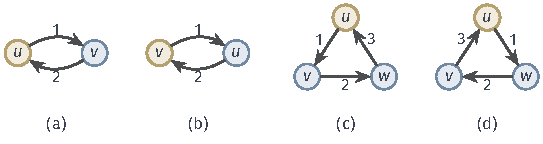
\includegraphics{figures/03-graphs/05-matrices-and-spectra/tikz/adjacency-edge-triangle-walks/figure.pdf}
  \caption{简单图上的两步与三步闭行走计数。浅黄色顶点标出闭行走的起点，箭头旁数字为步序。(a)(b) 同一条无向边$\{u,v\}$分别以$u$和$v$为起点各产生一条两步往返闭行走，共$2$条。(c)(d) 同一个三角形$\{u,v,w\}$在固定起点$u$下有顺、逆两个绕行方向；换遍三个起点共产生$3\times 2=6$条三步闭行走。}
  \label{fig:adjacency-edge-triangle-walks}
\end{BookInlineFigure}

记$t_3$为图$\mathcal G$中三角形（无序三元子集）的个数，则全图三步闭行走总数为$6t_3$。由此，图的边数$m$与三角形个数$t_3$可完全由二阶与三阶谱矩直接算出：
\begin{equation}
m=\frac12\operatorname{tr}(\bm A^2)=\frac12\sum_{i=1}^n\lambda_i^2,
\qquad
t_3=\frac16\operatorname{tr}(\bm A^3)=\frac16\sum_{i=1}^n\lambda_i^3.
\label{eq:adjacency-edge-triangle-counts}
\end{equation}

我们在四点环加对角边$\{1,3\}$的图上核对式~\eqref{eq:adjacency-edge-triangle-counts}。该图有$n=4$个顶点、$m=5$条边和$t_3=2$个三角形（即$\{1,2,3\}$与$\{1,3,4\}$）。其邻接矩阵$\bm A$与平方$\bm A^2$分别为
\[
\bm A=
\begin{bmatrix}
0&1&1&1\\
1&0&1&0\\
1&1&0&1\\
1&0&1&0
\end{bmatrix},
\qquad
\bm A^2=
\begin{bmatrix}
3&1&2&1\\
1&2&1&2\\
2&1&3&1\\
1&2&1&2
\end{bmatrix}.
\]
读取$\bm A^2$的四个对角元$(3,2,3,2)$，恰好是四个顶点的度$(d_1,d_2,d_3,d_4)$，二阶迹为$\operatorname{tr}(\bm A^2)=3+2+3+2=10$，除以$2$得边数$m=10/2=5$。再算$\bm A^3=\bm A^2\bm A$的对角元：例如$(\bm A^3)_{1,1}$是$\bm A^2$的第一行$(3,1,2,1)$与$\bm A$的第一列$(0,1,1,1)^\top$的内积，等于$1+2+1=4$（对应经过顶点$1$的两个三角形各贡献$2$个绕行方向）；同理可得$\bm A^3$的四个对角元为$(4,2,4,2)$，三阶迹为$\operatorname{tr}(\bm A^3)=4+2+4+2=12$，除以$6$得三角形数$t_3=12/6=2$。

\paragraph{四环数}

到了$k=4$步闭行走$v_0\to v_1\to v_2\to v_3\to v_0$，由于闭行走既可以沿简单四元环绕行，也可以在单条边或相邻两条边上来回折返，四阶谱矩$\operatorname{tr}(\bm A^4)$不再只包含四元环。按一条四步闭行走途中实际访问的不同顶点个数，可以将其不重不漏地分为三类（图~\ref{fig:adjacency-four-step-walks}）：
\begin{enumerate}
\item \textbf{第一类（只经过$2$个不同顶点）}：如图~\ref{fig:adjacency-four-step-walks}(a)所示，四步始终在同一条边$\{u,v\}$上来回折返两次。每条边有$u\to v\to u\to v\to u$和$v\to u\to v\to u\to v$两条记录，全图$m$条边共贡献$2m$条闭行走。
\item \textbf{第二类（经过$3$个不同顶点）}：如图~\ref{fig:adjacency-four-step-walks}(b)所示，在四个步序位置$v_0,v_1,v_2,v_3$中，必有某一个中心顶点$v$出现了两次，另外两个顶点$a,b$各出现一次（因无自环，重复顶点$v$只能隔一步出现在$v_0,v_2$或$v_1,v_3$位置，且$a,b$均与中心点$v$相邻，构成长为$2$的星形分支$a\text{--}v\text{--}b$）。对固定的一对公共邻居$\{a,b\}\subseteq N(v)$，共有$4$条四步闭行走：从中心$v$出发的$v\to a\to v\to b\to v$和$v\to b\to v\to a\to v$（$2$条），从端点$a$出发的$a\to v\to b\to v\to a$（$1$条），以及从端点$b$出发的$b\to v\to a\to v\to b$（$1$条）。在每个顶点$v\in V$处，从其$d_v$个邻居中选出一对无序邻居$\{a,b\}$共有$\binom{d_v}{2}$种选法，因此第二类闭行走总数为$4\sum_{v\in V}\binom{d_v}{2}$。
\item \textbf{第三类（经过$4$个不同顶点）}：如图~\ref{fig:adjacency-four-step-walks}(c)所示，四个顶点互不重复，首尾相连围成一个简单四元环$C_4$。设图中四元环的个数为$t_4$，每个四元环有$4$个可选起点、每个起点有顺逆$2$个绕行方向，共贡献$8t_4$条闭行走。
\end{enumerate}

\begin{BookInlineFigure}
  \centering
  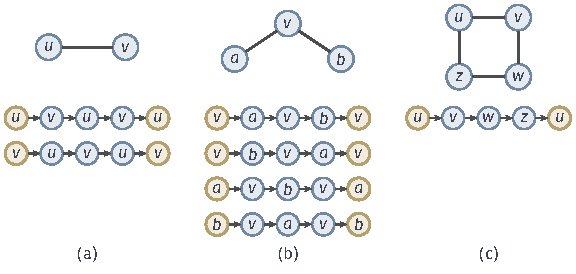
\includegraphics{figures/03-graphs/05-matrices-and-spectra/tikz/adjacency-four-step-walks/figure.pdf}
  \caption{按途中访问的不同顶点个数对四步闭行走分类。上排画出所使用的边，下排每一行从左到右列出一条五点访问序列，浅黄色标出重合的起点与终点。(a) 仅用$2$个顶点：在同一条边上来回折返两次（每条边$2$条）。(b) 使用$3$个顶点：在共享端点$v$的两条相邻边上各往返一次（每对相邻边$4$条）。(c) 使用$4$个不同顶点：沿简单四元环绕行一圈（每个四环$4\times 2=8$条）。}
  \label{fig:adjacency-four-step-walks}
\end{BookInlineFigure}

将三类闭行走条数相加，得到四阶谱矩分解公式：
\begin{equation}
\operatorname{tr}(\bm A^4)=\sum_{i=1}^n\lambda_i^4
=2m+4\sum_{v\in V}\binom{d_v}{2}+8t_4.
\label{eq:adjacency-four-cycle-count}
\end{equation}
在四点五边图上核对：第一类贡献$2m=10$；第二类中四个顶点的度依次为$3,2,3,2$，故$4\sum_v\binom{d_v}{2}=4\times(3+1+3+1)=32$；第三类中外圈$1\text{--}2\text{--}3\text{--}4\text{--}1$是唯一的四元环（$t_4=1$），贡献$8\times 1=8$；三项之和为$10+32+8=50$，与$\bm A^2$所有元素的平方和$\operatorname{tr}(\bm A^4)=\|\bm A^2\|_{\mathrm F}^2=(9+1+4+1)+(1+4+1+4)\times 2+(4+1+9+1)=50$完全一致。注意到式~\eqref{eq:adjacency-four-cycle-count}中出现了度平方和项$\sum_v\binom{d_v}{2}$：由于仅凭邻接谱一般无法唯一确定非正则图的度序列，从四阶谱矩$\operatorname{tr}(\bm A^4)$并不能单独反解出四元环个数$t_4$（第~\ref{sec:adjacency-cospectral-graphs}小节将给出具体反例）。

\subsection{直径的谱界}
\label{sec:adjacency-diameter-bound}

低阶谱矩刻画的是局部短闭行走。现在我们从另一个角度利用行走计数定理~\ref{thm:adjacency-walk-count}：如果图中两个顶点$u,v$之间的最短路距离为$k$，那么走少于$k$步绝对到不了$v$，而走恰好$k$步至少有一条路线能到达$v$。这一定性观察可以将图的全局直径与邻接矩阵不同特征值的个数联系起来。

回忆连通图$\mathcal G$中两点$u,v$之间的距离$\operatorname{dist}(u,v)$是连接它们的最短路径所含的边数，而图的直径$D=\max_{u,v\in V}\operatorname{dist}(u,v)$是所有点对距离的最大值。

取一对距离达到直径$D$的顶点，并写出连接它们的一条长度为$D$的最短路径：
\[
u_0\to u_1\to u_2\to\cdots\to u_D.
\]
对任意$k\in\{1,\ldots,D\}$，路径前缀$u_0\to u_1\to\cdots\to u_k$必然也是从$u_0$到$u_k$的最短路径（若存在少于$k$步的更短路径连接$u_0$与$u_k$，接上后缀$u_k\to\cdots\to u_D$就会得到一条总长小于$D$的从$u_0$到$u_D$的路径，与$\operatorname{dist}(u_0,u_D)=D$矛盾）。因此，$\operatorname{dist}(u_0,u_k)=k$。翻译成邻接矩阵幂的元素，就是：
\begin{equation}
(\bm A^j)_{u_0,u_k}=0\quad(\forall\,0\leq j<k),
\qquad\text{且}\qquad
(\bm A^k)_{u_0,u_k}\geq 1>0.
\label{eq:adjacency-diameter-echelon-entries}
\end{equation}
式~\eqref{eq:adjacency-diameter-echelon-entries}表明，$\bm I,\bm A,\bm A^2,\ldots,\bm A^D$这$D+1$个矩阵在一系列点对$(u_0,u_k)$处呈现出严格的“阶梯状”非零结构，由此可立即导出不同特征值个数的下界。

\begin{theorem}[直径的谱界]
\label{thm:adjacency-diameter-bound}
设连通简单无向图$\mathcal G$的直径为$D$，其邻接矩阵$\bm A$共有$r$个互不相同的特征值（不计重数）。则
\begin{equation}
r\geq D+1,\qquad\text{即}\qquad D\leq r-1.
\label{eq:adjacency-diameter-bound}
\end{equation}
\end{theorem}

\begin{proof}
我们分两步证明：（1）在$n\times n$矩阵空间中，$D+1$个矩阵幂$\bm I,\bm A,\bm A^2,\ldots,\bm A^D$线性无关；（2）若$\bm A$只有$r$个不同特征值，则$\bm A^r$可由$\bm I,\bm A,\ldots,\bm A^{r-1}$线性表出。

\textbf{第一步（$\bm I,\bm A,\ldots,\bm A^D$线性无关）}：用反证法。假设存在不全为零的实系数$c_0,c_1,\ldots,c_D$使得
\[
c_0\bm I+c_1\bm A+c_2\bm A^2+\cdots+c_D\bm A^D=\bm 0.
\]
令$k=\max\{j\in\{0,1,\ldots,D\}:c_j\neq 0\}$为最后一个非零系数的幂次，则上式化为
\[
c_0\bm I+c_1\bm A+\cdots+c_k\bm A^k=\bm 0,\qquad c_k\neq 0.
\]
在上面选出的最短路径$u_0\to u_1\to\cdots\to u_D$上，读取该矩阵等式在位置$(u_0,u_k)$处的元素：由式~\eqref{eq:adjacency-diameter-echelon-entries}，当$0\leq j<k$时$(\bm A^j)_{u_0,u_k}=0$，所有低次项在该位置全为$0$；唯一留下的最高次项为$c_k(\bm A^k)_{u_0,u_k}$。于是
\[
0=\sum_{j=0}^k c_j(\bm A^j)_{u_0,u_k}=c_k(\bm A^k)_{u_0,u_k}.
\]
但$c_k\neq 0$且$(\bm A^k)_{u_0,u_k}\geq 1>0$，乘积不可能等于$0$，矛盾。这证明了$\bm I,\bm A,\ldots,\bm A^D$这$D+1$个矩阵必定线性无关。

\textbf{第二步（利用特征根构造零化多项式）}：设$\bm A$的$r$个互不相同的实特征值为$\eta_1,\eta_2,\ldots,\eta_r$。构造$r$次首一多项式
\[
p(t)=(t-\eta_1)(t-\eta_2)\cdots(t-\eta_r)=t^r+b_{r-1}t^{r-1}+\cdots+b_1 t+b_0.
\]
因为实对称矩阵$\bm A$有一组由特征向量构成的完整正交基$\bm u_1,\ldots,\bm u_n$，每个基向量$\bm u_i$对应的特征值$\lambda_i$必定等于某个$\eta_j$。将矩阵多项式$p(\bm A)$作用在$\bm u_i$上，因子$(\bm A-\eta_j\bm I)\bm u_i=\bm 0$使整项归零：$p(\bm A)\bm u_i=\bm 0$（$\forall i=1,\ldots,n$）。在一个基上全为零的矩阵必为零矩阵，故
\[
p(\bm A)=\bm A^r+b_{r-1}\bm A^{r-1}+\cdots+b_1\bm A+b_0\bm I=\bm 0.
\]
这说明$\bm I,\bm A,\ldots,\bm A^r$这$r+1$个矩阵线性相关。若$r\leq D$，则$\{\bm I,\bm A,\ldots,\bm A^r\}$是线性无关组$\{\bm I,\bm A,\ldots,\bm A^D\}$的子集，不可能线性相关——矛盾。因此必有$r\geq D+1$。
\end{proof}

验证两个极端例子：完全图$K_n$（$n\geq 2$）的直径为$D=1$，定理~\ref{thm:adjacency-diameter-bound}要求它至少有$r\geq 2$个不同特征值，而第~\ref{sec:adjacency-complete-spectra}小节算出$K_n$恰有$n-1$和$-1$两个不同特征值（$r=2$），不等式取等；路径$P_n$的两端点距离为$D=n-1$，定理要求至少有$r\geq n$个不同特征值，因此$P_n$的全部$n$个特征值必定两两互异（单根），这与定理~\ref{prop:adjacency-path-spectrum}算出的$2\cos\bigl(\frac{k\pi}{n+1}\bigr)$完全一致。

\subsection{色数的谱界}
\label{sec:adjacency-chromatic-bounds}

图的正常顶点着色（proper vertex coloring）要求给每个顶点涂上一种颜色，使得任意一条边的两个端点颜色不同；所需的最少颜色数称为图的\emph{色数}（chromatic number），记为$\chi(\mathcal G)$。下面我们证明，仅凭最大特征值$\lambda_1$与最小特征值$\lambda_n$，就可以从上下两侧同时夹逼色数$\chi(\mathcal G)$。

在证明色数上界之前，需要先知道从图$\mathcal G$中删去若干顶点（连同关联的边）得到导出子图$\mathcal G'$时，邻接特征值如何变化。从矩阵上看，删去若干顶点相当于从邻接矩阵$\bm A$中删去相同编号的行和列，留下的子图邻接矩阵$\bm A_0$正是$\bm A$的一个主子矩阵（principal submatrix）。例如从三点路径$P_3$（特征值为$\sqrt 2,0,-\sqrt 2$）中删去端点$3$，留下的导出子图是单边图$K_2$（特征值为$1,-1$）。如图~\ref{fig:adjacency-interlacing-path}所示，$K_2$的两个特征值$1$和$-1$分别分别落在$P_3$相邻特征值所夹的区间$[0,\sqrt 2]$与$[-\sqrt 2,0]$内。

\begin{BookInlineFigure}
  \centering
  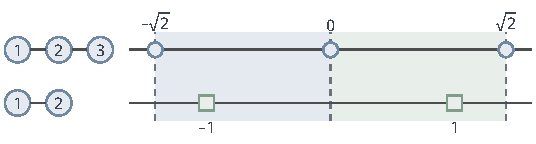
\includegraphics{figures/03-graphs/05-matrices-and-spectra/tikz/adjacency-interlacing-path/figure.pdf}
  \caption{删去三点路径$P_3$的端点$3$得到导出子图$K_2$时的特征值交错关系。上排圆点为$P_3$的邻接特征值$\sqrt2,0,-\sqrt2$，下排方点为二阶主子矩阵$K_2$的特征值$1,-1$，每个新特征值都落在相邻两个原特征值所夹的区间内。}
  \label{fig:adjacency-interlacing-path}
\end{BookInlineFigure}

这正是实对称矩阵的Cauchy交错定理（证明见\BookChapterRef{chap:condition-and-spectral-perturbation}{卷二"条件数与谱扰动"章}）：若$n$阶实对称矩阵$\bm A$的特征值为$\lambda_1\geq\cdots\geq\lambda_n$，其$k$阶主子矩阵$\bm A_0$的特征值为$\mu_1\geq\cdots\geq\mu_k$，则对每个$i=1,\ldots,k$都有$\lambda_i\geq\mu_i\geq\lambda_{i+n-k}$。特别地，取$i=1$可知：任意导出子图$\mathcal G'$的最大邻接特征值都不超过原图的最大邻接特征值，即$\lambda_1(\mathcal G')\leq\lambda_1(\mathcal G)$。需要注意，删顶点得到的是主子矩阵，可直接应用Cauchy交错定理；而单纯删边不删顶点只改变部分非对角元，并非主子矩阵截取。

有了导出子图的最大特征值界，下面同时证明色数$\chi(\mathcal G)$的Wilf上界与Hoffman下界。

\begin{theorem}[色数的谱上下界]
\label{thm:adjacency-chromatic-bounds}
设有限简单无向图$\mathcal G$至少含有一条边，色数为$\chi(\mathcal G)$，其最大与最小邻接特征值分别为$\lambda_1$与$\lambda_n$。则
\begin{equation}
1-\frac{\lambda_1}{\lambda_n}
\leq\chi(\mathcal G)
\leq 1+\lfloor\lambda_1\rfloor.
\label{eq:adjacency-chromatic-bounds}
\end{equation}
\end{theorem}

\begin{proof}
我们先证右侧上界$\chi(\mathcal G)\leq 1+\lfloor\lambda_1\rfloor$（Wilf界），再证左侧下界$\chi(\mathcal G)\geq 1-\lambda_1/\lambda_n$（Hoffman色数界）。

\textbf{第一步（上界证明：导出子图最小度与逆序贪心着色）}：任取原图$\mathcal G$的一个非空导出子图$\mathcal G'$，记其最小顶点度为$\delta(\mathcal G')$，平均度为$\overline d(\mathcal G')$。因为一组数的最小值不超过其平均值，且由定理~\ref{prop:adjacency-degree-bounds}（度下界）与主子矩阵Cauchy交错性质，有不等式链：
\[
\delta(\mathcal G')
\leq\overline d(\mathcal G')
\leq\lambda_1(\mathcal G')
\leq\lambda_1(\mathcal G)=\lambda_1.
\]
由于顶点度是整数，这保证了在$\mathcal G$的任意非空导出子图$\mathcal G'$中，总存在至少一个度不超过$\lfloor\lambda_1\rfloor$的顶点。

据此构造顶点删除序列：在原图$\mathcal G=\mathcal G_n$中选一个度$\leq\lfloor\lambda_1\rfloor$的顶点记为$v_n$并将其删去，得到$n-1$个顶点的导出子图$\mathcal G_{n-1}$；在$\mathcal G_{n-1}$中再选一个在$\mathcal G_{n-1}$内度$\leq\lfloor\lambda_1\rfloor$的顶点记为$v_{n-1}$并删去……如此继续，直到剩下一个顶点$v_1$。现在准备$\lfloor\lambda_1\rfloor+1$种颜色，按相反次序$v_1,v_2,\ldots,v_n$逐个将顶点放回并贪心着色：当放回顶点$v_j$时，它在已放回子图$\mathcal G_j=\{v_1,\ldots,v_j\}$中的邻居个数至多为$\lfloor\lambda_1\rfloor$，这些已着色的邻居至多占用了$\lfloor\lambda_1\rfloor$种颜色，因此在$\lfloor\lambda_1\rfloor+1$种颜色中必有至少一种空闲颜色可供$v_j$使用。故$\chi(\mathcal G)\leq 1+\lfloor\lambda_1\rfloor$。

\textbf{第二步（下界证明：单位根相位消去法）}：由于图至少有一条边，有$\lambda_1>0$；又因$\sum_{i=1}^n\lambda_i=\operatorname{tr}(\bm A)=0$，最小特征值必满足$\lambda_n<0$。

设图$\mathcal G$可以用$k=\chi(\mathcal G)$种颜色正常着色，将颜色编号为$c(u)\in\{0,1,\ldots,k-1\}$（$u\in V$），每条边$\{u,v\}\in E$的两端颜色不同：$c(u)\neq c(v)$。取$k$次本原单位根$\omega=\exp(2\pi\mathrm i/k)$，构造$n\times n$酉对角矩阵
\[
\begin{aligned}
\bm U&=\operatorname{diag}\bigl(\omega^{c(1)},\omega^{c(2)},\ldots,\omega^{c(n)}\bigr),\\
\bm U^*&=\bm U^{-1}=\operatorname{diag}\bigl(\omega^{-c(1)},\omega^{-c(2)},\ldots,\omega^{-c(n)}\bigr).
\end{aligned}
\]
对每个整数$j\in\{0,1,\ldots,k-1\}$，考察共轭矩阵$\bm U^{-j}\bm A\bm U^j$在位置$(u,v)$处的元素：
\[
\bigl(\bm U^{-j}\bm A\bm U^j\bigr)_{u,v}
=a_{u,v}\,\omega^{j(c(v)-c(u))}.
\]
将$j$从$0$到$k-1$对这$k$个矩阵求和：若$\{u,v\}\notin E$，则$a_{u,v}=0$，求和自然为$0$；若$\{u,v\}\in E$，因正常着色要求两端异色，$c(v)-c(u)\not\equiv 0\pmod k$，故公比$\eta=\omega^{c(v)-c(u)}\neq 1$且满足$\eta^k=1$，由等比数列求和公式有
\[
\sum_{j=0}^{k-1}\eta^j=\frac{1-\eta^k}{1-\eta}=0.
\]
这意味着在所有位置$(u,v)$上，$k$个共轭矩阵之和全为零矩阵：
\begin{equation}
\sum_{j=0}^{k-1}\bm U^{-j}\bm A\bm U^j=\bm 0.
\label{eq:adjacency-chromatic-phase-cancellation}
\end{equation}

现在取$\bm A$属于最大特征值$\lambda_1$的实单位特征向量$\bm x\in\mathbb R^n$（$\|\bm x\|_2=1$，$\bm x^\top\bm A\bm x=\lambda_1$），用$\bm x^\top$和$\bm x$夹乘式~\eqref{eq:adjacency-chromatic-phase-cancellation}两端，并令$\bm z^{(j)}=\bm U^j\bm x\in\mathbb C^n$：
\[
0=\sum_{j=0}^{k-1}\bm x^\top\bigl(\bm U^{-j}\bm A\bm U^j\bigr)\bm x
=\bm x^\top\bm A\bm x+\sum_{j=1}^{k-1}(\bm z^{(j)})^*\bm A\bm z^{(j)}.
\]
由于$\bm U^j$的对角元模长全为$1$，每个$\bm z^{(j)}=\bm U^j\bm x$仍是单位向量（$(\bm z^{(j)})^*\bm z^{(j)}=\|\bm x\|_2^2=1$）。在实对称矩阵$\bm A$的正交特征基下展开，任意复单位向量的二次型$(\bm z^{(j)})^*\bm A\bm z^{(j)}$都是特征值$\lambda_1,\ldots,\lambda_n$的凸组合，故不小于最小特征值$\lambda_n$。将$j=0$项的$\lambda_1$与其余$k-1$项的下界$\lambda_n$代入上式：
\[
0\geq\lambda_1+(k-1)\lambda_n.
\]
将负项$-(k-1)\lambda_n$移到左端并同除以$-\lambda_n>0$（注意$\lambda_n<0$），得$k-1\geq\frac{\lambda_1}{-\lambda_n}$，即$k\geq 1-\frac{\lambda_1}{\lambda_n}$。
\end{proof}

我们在完全图$K_n$和五元环$C_5$上检验定理~\ref{thm:adjacency-chromatic-bounds}。对完全图$K_n$，$\lambda_1=n-1,\lambda_n=-1$，下界给出$1-\frac{n-1}{-1}=n$，上界给出$1+\lfloor n-1\rfloor=n$，上下界同时取等，唯一确定$\chi(K_n)=n$。对五元奇环$C_5$，由定理~\ref{prop:adjacency-cycle-spectrum}知$\lambda_1=2$，$\lambda_5=2\cos(4\pi/5)=-\frac{1+\sqrt 5}{2}\approx -1.618$，下界给出
\[
\chi(C_5)\geq 1+\frac{2}{(1+\sqrt 5)/2}=1+\sqrt 5-1=\sqrt 5\approx 2.236.
\]
因为色数必须是整数，向上取整立得$\chi(C_5)\geq 3$；而上界给出$\chi(C_5)\leq 1+2=3$，上下界共同确定$\chi(C_5)=3$。

\subsection{独立数的谱界}
\label{sec:adjacency-hoffman-independence}

在图的正常着色中，涂同一种颜色的所有顶点彼此之间不能有边相连。这种两两互不相邻的顶点子集$S\subseteq V$称为图的\emph{独立集}（independent set），图所含最大独立集的顶点数称为\emph{独立数}（independence number），记为$\alpha(\mathcal G)$。显然，若用$\chi(\mathcal G)$种颜色把$n$个顶点分成$\chi(\mathcal G)$个独立集，每个独立集至多含$\alpha(\mathcal G)$个顶点，必有$n\leq\chi(\mathcal G)\alpha(\mathcal G)$，即$\chi(\mathcal G)\geq n/\alpha(\mathcal G)$。那么，能否直接用邻接谱给出独立数$\alpha(\mathcal G)$的上界？

如果直接取独立集$S$的$0$--$1$指示向量$\bm 1_S$（在$S$内取$1$、在$S$外取$0$），由于$S$内部没有任何边，二次型$\bm 1_S^\top\bm A\bm 1_S=0$恒等于零，从中读不出$|S|$的大小。为了把独立集向外部发出的边数信息引入二次型，同时也为了消去常向量$\bm 1$方向（最大特征值$\lambda_1=d$方向）的分量，我们在$d$正则图上从指示向量$\bm 1_S$中减去它的全图平均值$s/n$（其中$s=|S|$），构造中心化测试向量
\[
\bm x=\bm 1_S-\frac{s}{n}\bm 1.
\]
经过中心化后，$\bm x$在$S$内的$s$个顶点上取正值$1-\frac{s}{n}$，在$S$外的$n-s$个顶点上取负值$-\frac{s}{n}$，且全部$n$个分量之和为零（$\bm 1^\top\bm x=0$，即$\bm x\perp\bm 1$）。此时从$S$连向$V\setminus S$的跨界边两端一正一负，产生负的二次型，正好受最小特征值$\lambda_n$的下方约束。

\begin{theorem}[独立数的Hoffman界]
\label{thm:adjacency-hoffman-independence}
设$\mathcal G$是$n$个顶点的简单$d$正则无向图（$d\geq 1$），最小邻接特征值为$\lambda_n$。则其独立数$\alpha(\mathcal G)$满足
\begin{equation}
\alpha(\mathcal G)\leq n\,\frac{-\lambda_n}{d-\lambda_n}.
\label{eq:adjacency-hoffman-independence}
\end{equation}
\end{theorem}

\begin{proof}
任取$\mathcal G$的一个非空独立集$S\subseteq V$，记$s=|S|\geq 1$。因为$d\geq 1$，图中每个顶点都有边相连，独立集不可能包含全部顶点，故$1\leq s<n$。令$\bm x=\bm 1_S-\frac{s}{n}\bm 1$，则$\bm 1^\top\bm x=s-\frac{s}{n}\cdot n=0$，即$\bm x\in\bm 1^\perp$。

我们分别计算向量$\bm x$的欧氏长度平方$\|\bm x\|_2^2$和二次型$\bm x^\top\bm A\bm x$。首先计算长度平方：因为$\bm 1_S^\top\bm 1_S=s$且$\bm 1_S^\top\bm 1=s$，展开得
\[
\begin{aligned}
\|\bm x\|_2^2
&=\Bigl(\bm 1_S-\frac{s}{n}\bm 1\Bigr)^\top\Bigl(\bm 1_S-\frac{s}{n}\bm 1\Bigr)
=s-2\frac{s}{n}\cdot s+\frac{s^2}{n^2}\cdot n\\
&=s-\frac{s^2}{n}
=s\Bigl(1-\frac{s}{n}\Bigr)>0.
\end{aligned}
\]

再计算二次型$\bm x^\top\bm A\bm x$：利用双线性展开，
\[
\bm x^\top\bm A\bm x
=\bm 1_S^\top\bm A\bm 1_S
-2\frac{s}{n}\bm 1_S^\top\bm A\bm 1
+\frac{s^2}{n^2}\bm 1^\top\bm A\bm 1.
\]
逐项化简右端三项：第一项$\bm 1_S^\top\bm A\bm 1_S=\sum_{u,v\in S}a_{u,v}$等于独立集$S$内部边数的两倍，由于$S$是独立集、内部无边，故$\bm 1_S^\top\bm A\bm 1_S=0$；第二项利用$d$正则图的性质$\bm A\bm 1=d\bm 1$，得$\bm 1_S^\top\bm A\bm 1=d(\bm 1_S^\top\bm 1)=ds$；第三项同样由$\bm A\bm 1=d\bm 1$，得$\bm 1^\top\bm A\bm 1=d(\bm 1^\top\bm 1)=dn$。将三项结果代回，得到
\[
\bm x^\top\bm A\bm x
=0-2\frac{s}{n}(ds)+\frac{s^2}{n^2}(dn)
=-\frac{ds^2}{n}.
\]

现在应用Rayleigh商的最小特征值下界：对任意非零向量$\bm x$，都有$\bm x^\top\bm A\bm x\geq\lambda_n\|\bm x\|_2^2$。将上面算出的$\bm x^\top\bm A\bm x$与$\|\bm x\|_2^2$代入：
\[
-\frac{ds^2}{n}\geq\lambda_n\Bigl(s-\frac{s^2}{n}\Bigr).
\]
在不等式两端同除以正数$s>0$，得
\[
-\frac{ds}{n}\geq\lambda_n-\lambda_n\frac{s}{n}
\quad\Longrightarrow\quad
(d-\lambda_n)\frac{s}{n}\leq -\lambda_n.
\]
因为$d\geq 1$且$\lambda_n<0$，必有$d-\lambda_n>0$。两端同除以$d-\lambda_n$再乘以$n$，即得$s\leq n\frac{-\lambda_n}{d-\lambda_n}$。对最大独立集取$s=\alpha(\mathcal G)$，式~\eqref{eq:adjacency-hoffman-independence}得证。
\end{proof}

从证明过程还可以看到：在$d$正则图上，将式~\eqref{eq:adjacency-hoffman-independence}代入色数与独立数的关系$\chi(\mathcal G)\geq\frac{n}{\alpha(\mathcal G)}$，立得$\chi(\mathcal G)\geq\frac{d-\lambda_n}{-\lambda_n}=1-\frac{d}{\lambda_n}=1-\frac{\lambda_1}{\lambda_n}$，这从独立集视角再次印证了定理~\ref{thm:adjacency-chromatic-bounds}中的Hoffman色数下界。

检验两个例子：对偶数长环$C_{2r}$（$d=2,\lambda_n=-2$）或等侧完全二部图$K_{r,r}$（$d=r,\lambda_n=-r$），Hoffman界给出$\alpha(\mathcal G)\leq n\frac{d}{2d}=\frac{n}{2}$，取二部划分的任一侧即达到等号；对五元环$C_5$（$n=5,d=2,\lambda_5=-\frac{1+\sqrt 5}{2}$），Hoffman界给出$\alpha(C_5)\leq 5\cdot\frac{(1+\sqrt 5)/2}{2+(1+\sqrt 5)/2}=\sqrt 5\approx 2.236$，由于独立数是整数，向下取整得$\alpha(C_5)\leq 2$，任取两个不相邻顶点即达到最大值$2$。

\subsection{同谱图}
\label{sec:adjacency-spectral-information}
\label{sec:adjacency-cospectral-graphs}

综合前面几节的结果，我们可以对“完整邻接谱究竟能告诉我们多少图结构信息”作一全面梳理。

\paragraph{邻接谱确定的图不变量}

给定简单无向图$\mathcal G$的全部$n$个邻接特征值$\lambda_1\ge\cdots\ge\lambda_n$，以下不变量与界可由谱确定（界不等于相应参数的精确值）：
\begin{enumerate}
\item \textbf{顶点数$n$、边数$m$与三角形个数$t_3$}：特征值总个数就是顶点数$n$；由式~\eqref{eq:adjacency-edge-triangle-counts}，$m=\frac12\sum_{i=1}^n\lambda_i^2$，三角形个数$t_3=\frac16\sum_{i=1}^n\lambda_i^3$，以及任意阶$k$步闭行走的总数$\sum_{i=1}^n\lambda_i^k$。
\item \textbf{是否为正则图}：由定理~\ref{prop:adjacency-degree-bounds}，先由二阶谱矩算出平均度$\overline d=\frac1n\sum_{i=1}^n\lambda_i^2$，再检查最大特征值是否满足$\lambda_1=\overline d$。因为常向量$\bm 1$达到最大Rayleigh商$\lambda_1$当且仅当$\bm A\bm 1=\lambda_1\bm 1$（无论图是否连通），所以$\mathcal G$是正则图当且仅当$\lambda_1=\frac1n\sum_{i=1}^n\lambda_i^2$。
\item \textbf{是否为二部图}：由定理~\ref{thm:adjacency-bipartite-spectral-symmetry}的第1条，$\mathcal G$是二部图当且仅当全部特征值关于原点对称（$\lambda_i=-\lambda_{n+1-i},\forall i$）。
\item \textbf{直径、色数与独立数的硬性范围约束}：不同特征值个数给出连通图直径上界$D\leq r-1$，最大与最小特征值给出色数范围$1-\lambda_1/\lambda_n\leq\chi(\mathcal G)\leq 1+\lfloor\lambda_1\rfloor$及正则图独立数上界$\alpha(\mathcal G)\leq n\frac{-\lambda_n}{d-\lambda_n}$。
\end{enumerate}

\paragraph{同谱非同构图}

尽管邻接谱包含丰富的代数信息，但它不能唯一确定图的同构类。如果两张图$\mathcal G$与$\mathcal H$的邻接谱（作为带重数的多重集）完全相同，则称它们为\term{同谱图}（cospectral graphs，或等谱图）。两张同构的图仅相差顶点重新编号（即邻接矩阵相差置换相似变换$\bm P\bm A\bm P^\top$），因此必然同谱；但反过来，存在大量结构截然不同、却拥有完全相同邻接谱的非同构图。

最经典的一对五顶点同谱非同构图如图~\ref{fig:adjacency-cospectral-pair}所示：左图是星图$K_{1,4}$，右图是四元环与一个孤立顶点的不交并$C_4\sqcup K_1$。

\begin{figure}[!htb]
  \centering
  \begingroup
\definecolor{GraphSpectrumNode}{HTML}{E5EAF0}
\definecolor{GraphSpectrumOutline}{HTML}{7188A3}
\definecolor{GraphSpectrumEdge}{HTML}{4C4D4F}
\definecolor{GraphSpectrumText}{HTML}{3B4252}
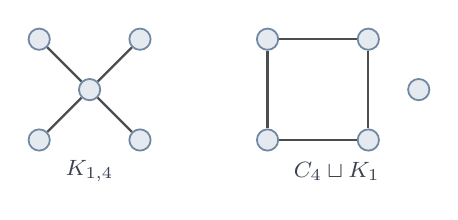
\begin{tikzpicture}[x=8mm,y=8mm,
  vertex/.style={circle,inner sep=0pt,minimum size=2.7mm,
    fill=GraphSpectrumNode,draw=GraphSpectrumOutline,line width=.65pt},
  every path/.style={line width=.8pt},
  title/.style={text=GraphSpectrumText,font=\footnotesize}]
  \begin{scope}
    \node[vertex] (s) at (0,0) {};
    \node[vertex] (l1) at (-.8,.8) {};
    \node[vertex] (l2) at (.8,.8) {};
    \node[vertex] (l3) at (.8,-.8) {};
    \node[vertex] (l4) at (-.8,-.8) {};
    \foreach \v in {l1,l2,l3,l4} {
      \draw[GraphSpectrumEdge] (s) -- (\v);
    }
    \node[title] at (0,-1.3) {$K_{1,4}$};
  \end{scope}
  \begin{scope}[xshift=29mm]
    \node[vertex] (c1) at (-.8,.8) {};
    \node[vertex] (c2) at (.8,.8) {};
    \node[vertex] (c3) at (.8,-.8) {};
    \node[vertex] (c4) at (-.8,-.8) {};
    \node[vertex] at (1.6,0) {};
    \draw[GraphSpectrumEdge] (c1) -- (c2) -- (c3) -- (c4) -- (c1);
    \node[title] at (.3,-1.3) {$C_4\sqcup K_1$};
  \end{scope}
\end{tikzpicture}
\endgroup

  \caption{最小的一对简单无向邻接同谱非同构图。(a) 左图星图$K_{1,4}$由$1$个中心顶点连接$4$个叶子顶点，连通且无环。(b) 右图$C_4\sqcup K_1$由一个四元环与一个孤立顶点组成，不连通且含四元环。两图的邻接谱同为$\{2,0,0,0,-2\}$。}
  \label{fig:adjacency-cospectral-pair}
\end{figure}

利用第~\ref{sec:adjacency-standard-spectra}节的结果立即可以核对两图的谱：左图$K_{1,4}$是$p=1,q=4$的完全二部图，由定理~\ref{prop:adjacency-bipartite-complete-spectrum}，其非零特征值为$\pm\sqrt{1\times 4}=\pm 2$，零特征值重数为$1+4-2=3$，故谱为$\{2,0,0,0,-2\}$；右图$C_4\sqcup K_1$是分块对角矩阵，$C_4$的特征值为$2,0,0,-2$，孤立顶点$K_1$添入一个特征值$0$，合起来的谱也是$\{2,0,0,0,-2\}$。

两张图的全部$5$个特征值一模一样，但它们展示出邻接谱丢失的三项重要结构信息：
\begin{enumerate}
\item \textbf{邻接谱不能判定连通性}：$K_{1,4}$是连通图（一棵树），而$C_4\sqcup K_1$不连通（有$2$个连通分量）。（第~\ref{chap:graph-laplacian-matrix}章将看到，拉普拉斯矩阵的零特征值重数恰等于连通分量个数，从而弥补邻接谱的这一缺陷。）
\item \textbf{邻接谱不能确定度序列}：$K_{1,4}$的度序列是$(4,1,1,1,1)$，而$C_4\sqcup K_1$的度序列是$(2,2,2,2,0)$。虽然两图的度之和都是$2m=8$，但各自的度分布完全不同。
\item \textbf{邻接谱不能确定四元环个数$t_4$}：$K_{1,4}$是树，四元环个数$t_4=0$；而$C_4\sqcup K_1$含有$t_4=1$个四元环。
\end{enumerate}

\paragraph{闭行走的补偿机制}

既然两图同谱，它们的任意阶谱矩$\operatorname{tr}(\bm A^k)=\sum_{i=1}^5\lambda_i^k$都相等，特别是四阶谱矩均为$\operatorname{tr}(\bm A^4)=2^4+(-2)^4=32$。为什么一张没有四元环（$t_4=0$）、另一张有一个四元环（$t_4=1$），四步闭行走的总数却同样是$32$？

用式~\eqref{eq:adjacency-four-cycle-count}把两图的四步闭行走按三类拆开：在星图$K_{1,4}$上，单边往返（第一类）有$2m=8$条，中心点度为$4$、有$\binom{4}{2}=6$对相邻边从而贡献$4\times 6=24$条星形分支往返（第二类），四元环绕行（第三类）为$8\times 0=0$条，合计$8+24+0=32$条。

而在$C_4\sqcup K_1$上，单边往返（第一类）也是$2m=8$条，四环上的$4$个顶点度均为$2$、各有$\binom{2}{2}=1$对相邻边从而只贡献$4\times(1+1+1+1)=16$条第二类行走，但多出的$1$个四元环恰好补上了$8\times 1=8$条第三类绕行，合计同样是$8+16+8=32$条。

可以看到，$K_{1,4}$靠度为$4$的中心节点多产生了$8$条三顶点折返行走，恰好与$C_4\sqcup K_1$沿四元环绕行产生的$8$条行走在求和后相抵。迹算子$\operatorname{tr}(\bm A^k)$只汇总闭行走的总条数，抹去了闭行走究竟来自星形高次度节点还是来自四元环的拓扑细节。

总结而言，邻接谱是图同构的一个必要非充分不变量：若两张图的邻接谱不同，立即可断定它们不同构；但若邻接谱相同，仅凭特征值还不足以确认同构。下一节我们将进一步考察：如果把原图的顶点按对称角色聚合成若干块，用更小的商矩阵代替原邻接矩阵，这种粗粒化的“商谱”又能保留多少谱信息？

\section{商谱}
\label{sec:adjacency-spectral-invariant}

完整邻接谱包含全部$n$个特征值，计算时需要处理$n\times n$矩阵。如果图中的顶点可以按连接角色分成$k$个块（$k\leq n$），使得同一块内的顶点对各个块具有完全相同的邻居计数，那么块与块之间的数值传递就可以用一个规模小得多的$k\times k$矩阵——商矩阵——来完整描述。从商矩阵算出的$k$个特征值称为图的商谱。

商谱并非对原图特征值的粗略数值近似，而是完整邻接谱中对应于“块内取常值”特征方向的精确子集。本节先定义等价划分、商矩阵与商谱，再说明颜色细化算法如何自动生成最粗的等价划分（即公平划分），最后严格证明商矩阵的实谱性质、不变子空间分解以及商谱对完整谱的精确嵌入定理。

\subsection{商矩阵}
\label{sec:adjacency-equitable-quotient}

我们先在四点环加对角边$\{1,3\}$的图上观察一种特殊的分块赋值现象。把度为$3$的两个对角顶点归为第一块$C_1=\{1,3\}$，把度为$2$的另外两个顶点归为第二块$C_2=\{2,4\}$。如图~\ref{fig:adjacency-quotient-block-values}(a)所示，给$C_1$中的顶点$1,3$统一赋读数$a$，给$C_2$中的顶点$2,4$统一赋读数$b$，构成块常值向量$\bm x=(a,b,a,b)^\top$。

现在对$\bm x$施加一次邻接矩阵$\bm A$，逐点查看邻居读数之和：在第一块$C_1$中，顶点$1$的三个邻居是$3\in C_1$（读数$a$）以及$2,4\in C_2$（读数各为$b$），邻居和为$1\cdot a+2\cdot b=a+2b$，顶点$3$的三个邻居是$1\in C_1$和$2,4\in C_2$，邻居和同样为$a+2b$。

在第二块$C_2$中，顶点$2$和顶点$4$的两个邻居都是$1,3\in C_1$（读数各为$a$）、在$C_2$内部没有邻居，故邻居和同为$2\cdot a+0\cdot b=2a$。如图~\ref{fig:adjacency-quotient-block-values}(b)所示，经过邻接矩阵作用后，同一块内的顶点依然保持相同的输出值。第一块统一从$a$更新为$a+2b$，第二块统一从$b$更新为$2a$。这意味着我们无需再逐个追踪全部$4$个顶点，只需用一个$2\times 2$小矩阵就能直接写出两块代表值$(a,b)^\top$的更新规则：
\[
\begin{bmatrix}1&2\\2&0\end{bmatrix}
\begin{bmatrix}a\\b\end{bmatrix}
=\begin{bmatrix}a+2b\\2a\end{bmatrix}.
\]

\begin{BookInlineFigure}
  \centering
  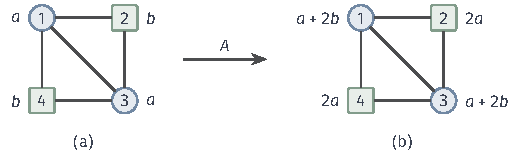
\includegraphics{figures/03-graphs/05-matrices-and-spectra/tikz/adjacency-quotient-block-values/figure.pdf}
  \caption{四点五边图上的块常值赋值与邻接更新。(a) 圆形顶点$C_1=\{1,3\}$统一赋读数$a$，方形顶点$C_2=\{2,4\}$统一赋读数$b$。(b) 经邻接矩阵$\bm A$作用后，$C_1$内每个顶点同取$a+2b$，$C_2$内每个顶点同取$2a$，输出仍为块常值向量。}
  \label{fig:adjacency-quotient-block-values}
\end{BookInlineFigure}

为什么同块内的顶点在乘$\bm A$之后还能保持取值一致？关键在于：同一个块$C_i$中的每一个顶点，落在任意块$C_j$中的邻居个数都是同一个常数。把这一结构条件提炼出来，就得到等价划分与商矩阵的定义。

\begin{definition}[等价划分与商矩阵]
\label{def:adjacency-equitable-partition}
设$\mathcal P=\{C_1,\ldots,C_r\}$是图$\mathcal G=(V,E)$顶点集$V$的一个划分（各块$C_i$非空且互不相交）。若对任意一对下标$i,j\in\{1,\ldots,r\}$（允许$i=j$），块$C_i$中的每一个顶点$u\in C_i$在块$C_j$中所拥有的邻居个数都等于同一个常数$q_{i,j}$（即$\bigl|N(u)\cap C_j\bigr|=q_{i,j}$仅依赖于$i,j$而与$u\in C_i$的具体选取无关），则称$\mathcal P$为图$\mathcal G$的一个\term{等价划分}（equitable partition）。由块间邻居计数$q_{i,j}$排成的$r\times r$矩阵$\bm Q=(q_{i,j})\in\mathbb R^{r\times r}$称为该等价划分的\term{商矩阵}（quotient matrix），$\bm Q$的全部特征值组成的多重集$\operatorname{spec}(\bm Q)$称为对应的\term{商谱}（quotient spectrum）。
\end{definition}

在上面四点五边图的划分$C_1=\{1,3\},C_2=\{2,4\}$中，$q_{1,1}=1,q_{1,2}=2,q_{2,1}=2,q_{2,2}=0$，商矩阵正是
\[
\bm Q=
\begin{bmatrix}
1&2\\
2&0
\end{bmatrix}.
\]
解二次特征方程$\det(\lambda\bm I-\bm Q)=\lambda(\lambda-1)-4=\lambda^2-\lambda-4=0$，立得商谱为
\[
\operatorname{spec}(\bm Q)=\left\{\frac{1+\sqrt{17}}{2},\;\frac{1-\sqrt{17}}{2}\right\}.
\]
原图的完整邻接谱有$4$个特征值，而商谱给出了其中$2$个——那么怎样在一般图上自动寻找这样的划分？另外$2$个特征值又藏在哪里？下面两小节依次回答这两个问题。

\subsection{公平划分}
\label{sec:adjacency-color-refinement-partition}

上一小节从分块矩阵的邻居计数定义了等价划分，但一张图往往存在不止一个等价划分（例如把每个顶点各自单独作为一块，总是包含$n$块的平凡等价划分）。在图算法中，我们希望从没有任何先验区分的统一初色出发，完全依靠图的局部连接结构自动划分出最精简的顶点类别。为此，先从顶点着色（色类）的角度给出公平划分的定义。

\begin{definition}[公平划分]
\label{def:fair-partition}
设图$\mathcal G=(V,E)$的顶点集$V$被划分为$k$个互不相交的非空子集（称为色类或单元）：
\[
V=C_1\cup C_2\cup\cdots\cup C_k.
\]
称该划分为图$\mathcal G$的一个\term{公平划分}（fair partition），如果对任意两个色类$C_i$与$C_j$（$1\leq i,j\leq k$，$i$与$j$可相同也可不同），色类$C_i$中的任意顶点$u\in C_i$在色类$C_j$中的邻居个数都等于一个固定常数$b_{i,j}=\bigl|N(u)\cap C_j\bigr|$，该常数仅取决于色类对$(C_i,C_j)$，而与顶点$u\in C_i$的具体选择无关。
\end{definition}

对比定义~\ref{def:adjacency-equitable-partition}与定义~\ref{def:fair-partition}可以看出，公平划分与等价划分所要求的块间邻居计数条件（$b_{i,j}=q_{i,j}$）在数学上完全一致。本章把这两个名称作为同义表述，不以构造方式区分它们。颜色细化的稳定划分是其中一个特殊成员，须另行证明其最粗性。下面我们依次证明：颜色细化的稳定划分必为公平划分，且它是图上所有等价划分中最粗（块数最少）的那一个。

\subsubsection{颜色细化的稳定划分}
\label{sec:adjacency-color-refinement-stable}

回顾第~\ref{sec:graph-wl-refinement}节的颜色细化算法：初始时（第$0$轮），给图中所有顶点赋同一种初始颜色；在每一轮迭代中，同时检验每个顶点当前的自身颜色以及它在各个当前色类中的邻居个数（合称为该顶点的颜色签名），只有自身颜色相同且对每种颜色的邻居个数也完全相同的顶点，才在下一轮归入同一个新色类，否则就被拆分成不同的色类。由于每次拆分都会使色类的个数严格增加，而$n$个顶点至多只能拆成$n$个单点色类，因此迭代必然在有限步（至多$n-1$轮拆分）内达到稳定状态——即再执行一轮细化，色类划分不再发生任何改变。

图~\ref{fig:adjacency-color-refinement-steps}展示了四点五边图从统一初色出发的颜色细化过程：
\begin{itemize}
\item \textbf{第$0$轮（统一初色）}：如图~\ref{fig:adjacency-color-refinement-steps}(a)所示，四个顶点$\{1,2,3,4\}$全部涂成同一种初始颜色（色$0$）。
\item \textbf{第$1$轮（按度分色）}：如图~\ref{fig:adjacency-color-refinement-steps}(b)所示，统计每个顶点在色$0$中的邻居个数（即顶点度）：顶点$1,3$各有$3$个色$0$邻居（$d=3$），顶点$2,4$各有$2$个色$0$邻居（$d=2$）。于是顶点集分裂为两个色类$C_1=\{1,3\}$（蓝圆）与$C_2=\{2,4\}$（绿方）。
\item \textbf{第$2$轮（核对邻居色分布并稳定）}：如图~\ref{fig:adjacency-color-refinement-steps}(c)所示，分别统计每个顶点在$(C_1,C_2)$两个色类中的邻居个数：$C_1$中的顶点$1$和$3$在$(C_1,C_2)$中的邻居个数同为$(1,2)$；$C_2$中的顶点$2$和$4$在$(C_1,C_2)$中的邻居个数同为$(2,0)$。同一色类内部的所有顶点具有完全相同的邻居计数签名，不再发生任何拆分，算法稳定于划分$\mathcal P_{\mathrm{stable}}=\bigl\{\{1,3\},\{2,4\}\bigr\}$。
\end{itemize}
又如在六元环$C_6$（或任意$d$正则图）上，第$0$轮所有顶点同为色$0$，第$1$轮每个顶点都有$d=2$个色$0$邻居，签名完全相同，从第一步起就不再分裂，稳定划分只有一个色类$C_1=V$。

\begin{BookInlineFigure}
  \centering
  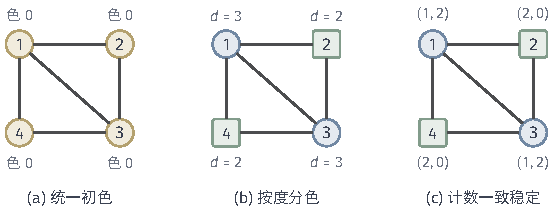
\includegraphics{figures/03-graphs/05-matrices-and-spectra/tikz/adjacency-color-refinement-steps/figure.pdf}
  \caption{四点五边图上的颜色细化稳定过程。(a) 第$0$轮：所有顶点赋统一初色（色$0$）。(b) 第$1$轮：按色$0$邻居数（即顶点度）拆分为度$3$色类$C_1=\{1,3\}$（蓝圆）与度$2$色类$C_2=\{2,4\}$（绿方）。(c) 第$2$轮：$C_1$内各点对$(C_1,C_2)$的邻居计数均为$(1,2)$，$C_2$内各点均为$(2,0)$，划分达到稳定。}
  \label{fig:adjacency-color-refinement-steps}
\end{BookInlineFigure}

下面的定理说明，颜色细化停止（稳定）的那一刻，所得的色类划分自动满足公平划分的定义。

\begin{theorem}[颜色细化的稳定划分是公平划分]
\label{thm:stable-is-equitable}
对任意有限简单无向图$\mathcal G=(V,E)$，从统一初色出发运行颜色细化算法，达到稳定时的色类划分$\mathcal P_{\mathrm{stable}}=\{C_1,\ldots,C_k\}$必为图$\mathcal G$的公平划分。
\end{theorem}

\begin{proof}
设算法在达到稳定划分$\mathcal P_{\mathrm{stable}}=\{C_1,\ldots,C_k\}$后再执行一轮核对。任取两个色类$C_i,C_j\in\mathcal P_{\mathrm{stable}}$，并任取色类$C_i$中的两个顶点$u,v\in C_i$。

因为划分$\mathcal P_{\mathrm{stable}}$已经稳定，再执行一轮颜色细化不会把同属$C_i$的顶点$u$和$v$拆入不同的新色类。根据颜色细化的更新规则，两个同色顶点$u,v$在下一轮保持同色，当且仅当它们在每一个当前色类$C_\ell$（$\ell=1,\ldots,k$）中的邻居个数都分别相等。特别地，取$\ell=j$，即有
\[
\bigl|N(u)\cap C_j\bigr|=\bigl|N(v)\cap C_j\bigr|.
\]
由于$u,v\in C_i$是任意选取的，这说明$C_i$中所有顶点在$C_j$中的邻居个数都等于同一个常数$b_{i,j}$。由定义~\ref{def:fair-partition}，$\mathcal P_{\mathrm{stable}}$是公平划分。
\end{proof}

\subsubsection{最粗等价划分}
\label{sec:adjacency-coarsest-equitable-partition}

既然公平划分与等价划分满足相同的块间邻居计数条件，为什么由颜色细化生成的公平划分在所有等价划分中地位最特殊？答案是：它合并了尽可能多的“结构角色不可区分”的顶点，是图上所有等价划分中最粗（块数最少）的那一个。为了严格表述这一结论，我们先定义两个划分之间的细化偏序关系。

\begin{definition}[划分的细化]
\label{def:partition-refinement}
设$\mathcal P=\{D_1,\ldots,D_r\}$与$\mathcal P'=\{C_1,\ldots,C_k\}$是同一顶点集$V$上的两个划分。若$\mathcal P$中的每一个块$D_a$都完整地包含在$\mathcal P'$的某一个块$C_i$之内（即对每个$a\in\{1,\ldots,r\}$，存在$i\in\{1,\ldots,k\}$使得$D_a\subseteq C_i$），则称划分$\mathcal P$是划分$\mathcal P'$的\term{细化}（refinement），或称$\mathcal P'$比$\mathcal P$更粗（coarser）。若$\mathcal P$是$\mathcal P'$的细化且$\mathcal P\neq\mathcal P'$，则称$\mathcal P$是$\mathcal P'$的严格细化。
\end{definition}

根据定义~\ref{def:partition-refinement}，说$\mathcal P$是$\mathcal P'$的细化，直观上就是指$\mathcal P$可以通过把$\mathcal P'$的某些块进一步切碎得到；等价地，$\mathcal P'$的每一个块$C_i$都恰好是$\mathcal P$中若干个完整块的并集。例如在四点集$\{1,2,3,4\}$上，$\mathcal P=\bigl\{\{1\},\{2\},\{3,4\}\bigr\}$是$\mathcal P'=\bigl\{\{1,2\},\{3,4\}\bigr\}$的细化（将$\{1,2\}$拆成了$\{1\}$和$\{2\}$）；而$\bigl\{\{1,3\},\{2,4\}\bigr\}$不是$\mathcal P'$的细化，因为块$\{1,3\}$横跨了$\mathcal P'$的两个块。在全体划分中，最细的划分是每个顶点各自成一块的单点划分（共$n$块），最粗的划分是全体顶点合成一块的整图划分（仅$1$块）。

现在我们证明：任何等价划分都是颜色细化稳定划分的细化。

\begin{theorem}[统一初色的稳定划分是最粗等价划分]
\label{thm:color-refinement-coarsest}
设$\mathcal P_{\mathrm{stable}}=\{C_1,\ldots,C_k\}$是从统一初色出发运行颜色细化得到的稳定公平划分，$\mathcal P=\{D_1,\ldots,D_r\}$是图$\mathcal G$的任意一个等价划分。则$\mathcal P$必为$\mathcal P_{\mathrm{stable}}$的细化（即$\mathcal P_{\mathrm{stable}}$是图$\mathcal G$最粗的等价划分，并在不计块的排列次序下唯一确定）。
\end{theorem}

\begin{proof}
记$\mathcal P^{(t)}$为颜色细化第$t$轮结束时的色类划分（$t=0,1,2,\ldots$）。我们对轮数$t$作数学归纳法，证明对一切$t\geq 0$，$\mathcal P$都是$\mathcal P^{(t)}$的细化——即颜色细化在任何一轮都不会把等价划分$\mathcal P$的同一个块$D_a$中的两个顶点拆开。

\textbf{归纳基础（$t=0$）}：第$0$轮为统一初色，$\mathcal P^{(0)}=\{V\}$只有一个块。对任意$D_a\in\mathcal P$，显然有$D_a\subseteq V$，故$\mathcal P$是$\mathcal P^{(0)}$的细化。

\textbf{归纳步骤}：假设第$t$轮结束时$\mathcal P$是$\mathcal P^{(t)}$的细化。这意味着$\mathcal P^{(t)}$中的每一个当前色类$C\in\mathcal P^{(t)}$，都恰好是$\mathcal P$中若干个完整块的并集。

现在考察第$t+1$轮的颜色更新。任取$\mathcal P$的一个块$D_a\in\mathcal P$，并任取其中的两个顶点$u,v\in D_a$。由归纳假设，$u$和$v$在第$t$轮属于同一个色类，具有相同的第$t$轮颜色。要证明它们在第$t+1$轮仍然获得相同颜色，只需证明对$\mathcal P^{(t)}$中的任意一个色类$C\in\mathcal P^{(t)}$，$u$和$v$在$C$中的邻居个数相等。

由于$C\in\mathcal P^{(t)}$是$\mathcal P$中若干个互不相交块的并集，设
\[
C=D_{b_1}\cup D_{b_2}\cup\cdots\cup D_{b_s}.
\]
因为$\mathcal P=\{D_1,\ldots,D_r\}$是等价划分（商矩阵记为$q_{a,b}$），块$D_a$中的任意顶点在块$D_{b_\ell}$中的邻居个数都等于固定常数$q_{a,b_\ell}$。由于$D_{b_1},\ldots,D_{b_s}$互不相交，顶点$u\in D_a$在并集$C$中的邻居总数为
\[
\bigl|N(u)\cap C\bigr|
=\sum_{\ell=1}^s\bigl|N(u)\cap D_{b_\ell}\bigr|
=q_{a,b_1}+q_{a,b_2}+\cdots+q_{a,b_s}.
\]
完全相同地，顶点$v\in D_a$在$C$中的邻居总数也为
\[
\bigl|N(v)\cap C\bigr|
=\sum_{\ell=1}^s\bigl|N(v)\cap D_{b_\ell}\bigr|
=q_{a,b_1}+q_{a,b_2}+\cdots+q_{a,b_s}
=\bigl|N(u)\cap C\bigr|.
\]
这对所有色类$C\in\mathcal P^{(t)}$均成立，故$u$和$v$在第$t+1$轮的颜色签名完全一致，仍然留在同一个第$t+1$轮色类中。因此，块$D_a$的全体顶点整体包含在$\mathcal P^{(t+1)}$的某个色类中，即$\mathcal P$也是$\mathcal P^{(t+1)}$的细化。

由数学归纳法，当算法在有限步达到稳定划分$\mathcal P_{\mathrm{stable}}$时，$\mathcal P$仍是$\mathcal P_{\mathrm{stable}}$的细化。
\end{proof}

定理~\ref{thm:color-refinement-coarsest}给出了一个构造结论：我们不需要靠人工猜测去寻找等价划分，只需从统一初色运行确定性的颜色细化算法，就一定能找到全图最粗、块数最少（从而商矩阵维数最小）的规范公平划分$\mathcal P_{\mathrm{stable}}$。当需要判断两张图$\mathcal G$和$\mathcal H$是否可能同构时，可以在它们的不交并$\mathcal G\sqcup\mathcal H$上使用同一套颜色编码同步运行颜色细化：若两图同构，稳定后每个色类在两图中的顶点数$|C_i|$以及块间邻居计数$b_{i,j}$必定完全匹配，导出相同的公平划分商矩阵$\bm Q$；反之，只要色类大小或商矩阵不匹配，立即可断定两图不同构。

\subsection{公平划分的性质}
\label{sec:adjacency-spectral-hierarchy}

找到公平划分$\mathcal P=\{C_1,\ldots,C_k\}$及其$k\times k$商矩阵$\bm Q=(b_{i,j})$之后，一个核心的谱图论问题是：这个小矩阵$\bm Q$的特征值（商谱）与原图$n\times n$邻接矩阵$\bm A$的特征值（完整邻接谱）之间究竟有什么关系？下面我们分三个子小节，通过形式化定理和严格证明逐一揭示商矩阵的实谱性质、块常值不变子空间交织恒等式以及商谱对完整谱的精确嵌入分解，并剖析商谱保留与丢失的结构信息。

\subsubsection{商矩阵的实谱}
\label{sec:adjacency-quotient-real-spectrum}

首先，对给定的图$\mathcal G$，一般的等价划分可以有很多个，各自导出不同阶数的商矩阵；但根据定理~\ref{thm:color-refinement-coarsest}，从统一初色出发由颜色细化生成的公平划分$\mathcal P=\{C_1,\ldots,C_k\}$作为最粗等价划分是唯一确定的。因此，在不计$k$个色类排列顺序（即对$\bm Q$的行和列同时施加相同置换$\bm P\bm Q\bm P^\top$）的意义下，公平划分导出的商矩阵$\bm Q$及其商谱$\operatorname{spec}(\bm Q)$是图$\mathcal G$唯一确定的代数不变量。

其次，观察商矩阵$\bm Q=(b_{i,j})$的形式：虽然原图的邻接矩阵$\bm A$是对称矩阵，但商矩阵$\bm Q$通常不是对称矩阵。例如在三点路径$1\text{--}2\text{--}3$上，公平划分将两个度为$1$的端点归为第一块$C_1=\{1,3\}$（$|C_1|=2$），将度为$2$的中心点归为第二块$C_2=\{2\}$（$|C_2|=1$）。此时，$C_1$中的每个端点在$C_2$中只有$b_{1,2}=1$个邻居，而$C_2$中的中心点在$C_1$中却有$b_{2,1}=2$个邻居，商矩阵为
\[
\bm Q=\begin{bmatrix}0&1\\2&0\end{bmatrix},\qquad b_{1,2}=1\neq 2=b_{2,1}.
\]
既然$\bm Q$不对称，它的特征值会不会出现复数？能不能对角化？下面的定理通过“双向计数跨块边数”证明：商矩阵$\bm Q$虽然自身未必对称，但通过块大小对角矩阵作一次对角相似变换，就能变成实对称矩阵。

\begin{theorem}[商矩阵的实谱性质]
\label{thm:quotient-matrix-real-spectrum}
设$\mathcal P=\{C_1,\ldots,C_k\}$是有限简单无向图$\mathcal G=(V,E)$的一个公平划分（或任意等价划分），商矩阵为$\bm Q=(b_{i,j})\in\mathbb R^{k\times k}$，记块大小对角矩阵为
\[
\bm D_C=\operatorname{diag}\bigl(|C_1|,|C_2|,\ldots,|C_k|\bigr).
\]
则块大小与商矩阵满足对称平衡恒等式
\begin{equation}
|C_i|\,b_{i,j}=|C_j|\,b_{j,i}\quad(\forall\,1\leq i,j\leq k),
\qquad\text{即}\qquad
\bm D_C\bm Q=\bm Q^\top\bm D_C.
\label{eq:adjacency-quotient-symmetry}
\end{equation}
进一步，矩阵
\[
\widetilde{\bm Q}=\bm D_C^{1/2}\bm Q\bm D_C^{-1/2}
\]
是$k\times k$实对称矩阵。因此，商矩阵$\bm Q$在实数域$\mathbb R$上可对角化，其全部$k$个特征值均为实数。
\end{theorem}

\begin{proof}
任取两个色类$C_i$与$C_j$（当$i=j$时$|C_i|b_{i,i}=|C_j|b_{j,i}$恒成立；以下设$i\neq j$），我们从左右两侧分别计算横跨在$C_i$与$C_j$之间的无向边总数$e(C_i,C_j)$：从$C_i$一侧计数，$C_i$中共有$|C_i|$个顶点，由公平划分定义，其中每一个顶点在$C_j$中都恰好有$b_{i,j}$个邻居，故跨块边总数为$e(C_i,C_j)=|C_i|\,b_{i,j}$；从$C_j$一侧计数，$C_j$中共有$|C_j|$个顶点，其中每一个顶点在$C_i$中都恰好有$b_{j,i}$个邻居，故同一批跨块边的总数又等于$e(C_i,C_j)=|C_j|\,b_{j,i}$。两边相等即得$|C_i|\,b_{i,j}=|C_j|\,b_{j,i}$。注意到$(\bm D_C\bm Q)_{i,j}=|C_i|b_{i,j}$，而$(\bm Q^\top\bm D_C)_{i,j}=(\bm Q^\top)_{i,j}|C_j|=b_{j,i}|C_j|$，故矩阵等式$\bm D_C\bm Q=\bm Q^\top\bm D_C$成立，式~\eqref{eq:adjacency-quotient-symmetry}得证。

由于每个色类$C_i$非空，$|C_i|\geq 1>0$，对角矩阵
\[
\bm D_C^{1/2}=\operatorname{diag}\bigl(\sqrt{|C_1|},\ldots,\sqrt{|C_k|}\bigr)
\]
及其逆矩阵$\bm D_C^{-1/2}$均为实可逆对角矩阵。对$\bm D_C\bm Q=\bm Q^\top\bm D_C$两端左乘$\bm D_C^{-1/2}$、右乘$\bm D_C^{-1/2}$，得到
\[
\bm D_C^{1/2}\bm Q\bm D_C^{-1/2}
=\bm D_C^{-1/2}\bm Q^\top\bm D_C^{1/2}
=\bigl(\bm D_C^{1/2}\bm Q\bm D_C^{-1/2}\bigr)^\top,
\]
这证明了$\widetilde{\bm Q}=\bm D_C^{1/2}\bm Q\bm D_C^{-1/2}$是实对称矩阵（其第$(i,j)$个元素为$b_{i,j}\sqrt{|C_i|/|C_j|}=b_{j,i}\sqrt{|C_j|/|C_i|}$）。

由实对称矩阵谱定理，$\widetilde{\bm Q}$有$k$个实特征值和一组标准正交实特征向量基$\tilde{\bm y}_1,\ldots,\tilde{\bm y}_k$。因为$\bm Q=\bm D_C^{-1/2}\widetilde{\bm Q}\bm D_C^{1/2}$与实对称矩阵$\widetilde{\bm Q}$相似，二者具有完全相同的特征多项式与实特征值，且$\bm y_r=\bm D_C^{-1/2}\tilde{\bm y}_r$（$r=1,\ldots,k$）构成$\bm Q$在$\mathbb R^k$中的一组线性无关实特征向量基，故$\bm Q$在$\mathbb R$上可对角化。
\end{proof}

\subsubsection{商谱嵌入}
\label{sec:adjacency-quotient-spectrum-embedding}

为了把$k\times k$商矩阵$\bm Q$与$n\times n$邻接矩阵$\bm A$连接起来，我们引入公平划分$\mathcal P=\{C_1,\ldots,C_k\}$的\emph{块指示矩阵}（characteristic matrix）$\bm S\in\mathbb R^{n\times k}$：其第$j$列就是色类$C_j$在顶点空间$\mathbb R^n$中的$0$--$1$指示向量$\bm 1_{C_j}$：
\[
S_{u,j}=(\bm 1_{C_j})_u=
\begin{cases}
1,& u\in C_j,\\
0,& u\notin C_j,
\end{cases}
\qquad 1\leq u\leq n,\;1\leq j\leq k.
\]
由于$C_1,\ldots,C_k$互不相交且非空，$\bm S$的各列在不同坐标集合上取$1$，满足
\[
\bm S^\top\bm S=\operatorname{diag}\bigl(|C_1|,\ldots,|C_k|\bigr)=\bm D_C,
\]
故$\bm S$列满秩（$\operatorname{rank}\bm S=k$）。

对任意块读数向量$\bm y=(y_1,\ldots,y_k)^\top\in\mathbb R^k$，左乘$\bm S$得到的$n$维向量
\[
\bm S\bm y=\sum_{j=1}^k y_j\,\bm 1_{C_j}\in\mathbb R^n
\]
在每个色类$C_j$的所有顶点上统一取常数值$y_j$。因此，$\bm S$的列空间
\[
\mathcal W=\operatorname{col}(\bm S)=\bigl\{\bm S\bm y:\bm y\in\mathbb R^k\bigr\}\subseteq\mathbb R^n
\]
是由全体“在每个色类内部取常值”的顶点向量组成的$k$维子空间，称为划分$\mathcal P$的\term{块常值子空间}（block-constant subspace）。而$\mathcal W$在$\mathbb R^n$中的正交补空间
\[
\mathcal W^\perp
=\ker(\bm S^\top)
=\Bigl\{\bm z\in\mathbb R^n:\bm 1_{C_j}^\top\bm z=\sum_{u\in C_j}z_u=0,\;\forall\,j=1,\ldots,k\Bigr\}
\]
则由全体“在每一个色类内部分量之和均为零”的顶点向量组成，维数为$n-k$。

下面的定理揭示了公平划分的本质代数特征：块常值子空间$\mathcal W$及其正交补$\mathcal W^\perp$都是邻接矩阵$\bm A$的不变子空间。

\begin{theorem}[商矩阵的交织恒等式]
\label{thm:quotient-intertwining}
设$\mathcal P=\{C_1,\ldots,C_k\}$是图$\mathcal G=(V,E)$的顶点集划分，$\bm S\in\mathbb R^{n\times k}$为其块指示矩阵。则$\mathcal P$是以$\bm Q=(b_{i,j})\in\mathbb R^{k\times k}$为商矩阵的公平划分（等价划分），当且仅当邻接矩阵$\bm A$与商矩阵$\bm Q$满足交织恒等式
\begin{equation}
\bm A\bm S=\bm S\bm Q.
\label{eq:adjacency-quotient-intertwining}
\end{equation}
在此条件下，块常值子空间$\mathcal W=\operatorname{col}(\bm S)$及其正交补空间$\mathcal W^\perp=\ker(\bm S^\top)$均为$\bm A$的不变子空间（即$\bm A\mathcal W\subseteq\mathcal W$且$\bm A\mathcal W^\perp\subseteq\mathcal W^\perp$）。
\end{theorem}

\begin{proof}
首先证明$\mathcal P$为商矩阵是$\bm Q$的公平划分当且仅当$\bm A\bm S=\bm S\bm Q$。任取顶点$u\in V$（设$u$属于色类$C_i$）和列下标$j\in\{1,\ldots,k\}$，分别计算式~\eqref{eq:adjacency-quotient-intertwining}左右两端在位置$(u,j)$处的元素。左端$\bm A\bm S$的第$j$列为$\bm A\bm 1_{C_j}$，其在顶点$u$处的元素为
\[
(\bm A\bm S)_{u,j}=(\bm A\bm 1_{C_j})_u=\sum_{v\in C_j}a_{u,v}=\bigl|N(u)\cap C_j\bigr|,
\]
即顶点$u$在色类$C_j$中的邻居个数；右端$\bm S\bm Q$在位置$(u,j)$处的元素为$\sum_{\ell=1}^k S_{u,\ell}\,b_{\ell,j}$，因为$u\in C_i$，只有$\ell=i$时$S_{u,i}=1$、其余$\ell\neq i$时$S_{u,\ell}=0$，故
\[
(\bm S\bm Q)_{u,j}=b_{i,j}.
\]
对比左右两端可知：$(\bm A\bm S)_{u,j}=(\bm S\bm Q)_{u,j}$对所有$u\in C_i$和所有$i,j$成立，当且仅当对任意$u\in C_i$都有$|N(u)\cap C_j|=b_{i,j}$，这正是定义~\ref{def:fair-partition}中公平划分的充要条件。

接下来证明$\mathcal W$与$\mathcal W^\perp$均为$\bm A$的不变子空间。一方面，对任意块常值向量$\bm w=\bm S\bm y\in\mathcal W$（$\bm y\in\mathbb R^k$），由交织恒等式~\eqref{eq:adjacency-quotient-intertwining}，有
\[
\bm A\bm w=\bm A(\bm S\bm y)=(\bm A\bm S)\bm y=\bm S(\bm Q\bm y)\in\operatorname{col}(\bm S)=\mathcal W,
\]
故$\bm A\mathcal W\subseteq\mathcal W$。另一方面，对任意$\bm z\in\mathcal W^\perp$和任意$\bm w\in\mathcal W$，由于$\bm A$是实对称矩阵（$\bm A^\top=\bm A$）且已证$\bm A\bm w\in\mathcal W$，有
\[
\langle\bm A\bm z,\bm w\rangle
=(\bm A\bm z)^\top\bm w
=\bm z^\top(\bm A\bm w)
=\langle\bm z,\bm A\bm w\rangle=0.
\]
这说明$\bm A\bm z$与$\mathcal W$中的一切向量正交，即$\bm A\bm z\in\mathcal W^\perp$，故$\bm A\mathcal W^\perp\subseteq\mathcal W^\perp$。定理得证。
\end{proof}

由定理~\ref{thm:quotient-intertwining}的交织恒等式$\bm A\bm S=\bm S\bm Q$，我们可以立即导出商谱与原图完整邻接谱之间的精确嵌合定理。

\begin{theorem}[商谱嵌入定理]
\label{thm:quotient-spectrum-inclusion}
设$\mathcal P=\{C_1,\ldots,C_k\}$是有限简单无向图$\mathcal G=(V,E)$的一个公平划分（或任意等价划分），块指示矩阵为$\bm S\in\mathbb R^{n\times k}$，商矩阵为$\bm Q\in\mathbb R^{k\times k}$。则：
\begin{enumerate}
\item 若$\bm y\in\mathbb R^k\setminus\{\bm 0\}$是商矩阵$\bm Q$属于特征值$\lambda$的特征向量（$\bm Q\bm y=\lambda\bm y$），则块常值向量$\bm S\bm y\in\mathcal W\setminus\{\bm 0\}$是原图邻接矩阵$\bm A$属于同一特征值$\lambda$的特征向量；
\item 按代数重数计，商矩阵的商谱$\operatorname{spec}(\bm Q)$等于$\bm A$限制在块常值子空间$\mathcal W$上的特征值多重集$\operatorname{spec}(\bm A|_{\mathcal W})$，从而完整包含在原图邻接谱中：
\[
\operatorname{spec}(\bm Q)\subseteq\operatorname{spec}(\bm A),\qquad
\operatorname{spec}(\bm A)=\operatorname{spec}(\bm Q)\,\cup\,\operatorname{spec}(\bm A|_{\mathcal W^\perp}),
\]
其中$\bm A$限制在正交补$\mathcal W^\perp$上的$n-k$个特征值$\operatorname{spec}(\bm A|_{\mathcal W^\perp})$称为该划分下的\term{剩余谱}（residual spectrum）；
\item 原图的最大邻接特征值$\lambda_1(\bm A)$必然包含在商谱$\operatorname{spec}(\bm Q)$中。
\end{enumerate}
\end{theorem}

\begin{proof}
\textbf{第1条与第2条}：因为$\bm S^\top\bm S=\bm D_C$可逆，线性映射$\bm S\colon\mathbb R^k\to\mathcal W$是双射（线性同构）：当$\bm y\neq\bm 0$时必有$\bm S\bm y\neq\bm 0$。若$\bm Q\bm y=\lambda\bm y$，由定理~\ref{thm:quotient-intertwining}的$\bm A\bm S=\bm S\bm Q$，立得
\[
\bm A(\bm S\bm y)=\bm S(\bm Q\bm y)=\bm S(\lambda\bm y)=\lambda(\bm S\bm y),
\]
即$\bm S\bm y\in\mathcal W$是$\bm A$属于特征值$\lambda$的特征向量。更进一步，式~\eqref{eq:adjacency-quotient-intertwining}表明线性算子$\bm A|_{\mathcal W}\colon\mathcal W\to\mathcal W$在基$\{\bm 1_{C_1},\ldots,\bm 1_{C_k}\}$下的表示矩阵恰好就是$\bm Q$，因此$\bm A|_{\mathcal W}$的特征多项式与$\bm Q$的特征多项式恒同，$\operatorname{spec}(\bm A|_{\mathcal W})=\operatorname{spec}(\bm Q)$（含重数）。又因$\mathbb R^n=\mathcal W\oplus\mathcal W^\perp$是$\bm A$的两个正交不变子空间的直和，在由$\mathcal W$的一组正交特征基与$\mathcal W^\perp$的一组正交特征基拼成的全空间正交基下，$\bm A$呈分块对角形$\operatorname{diag}(\bm A|_{\mathcal W},\bm A|_{\mathcal W^\perp})$，故完整邻接谱$\operatorname{spec}(\bm A)$等于商谱$\operatorname{spec}(\bm Q)$与剩余谱$\operatorname{spec}(\bm A|_{\mathcal W^\perp})$的并集。

\textbf{第3条（$\lambda_1(\bm A)\in\operatorname{spec}(\bm Q)$）}：由定理~\ref{thm:quotient-matrix-real-spectrum}，实对称矩阵$\widetilde{\bm Q}=\bm D_C^{1/2}\bm Q\bm D_C^{-1/2}$逐元素非负，与$\bm Q$（从而与$\bm A|_{\mathcal W}$）具有相同的最大特征值$\mu_{\max}=\lambda_1(\bm Q)$。在原图$\mathcal G$中取一个达到全图最大邻接特征值$\lambda_1(\bm A)$的连通分量$V_0$；当$V_0$至少含两个顶点时应用定理~\ref{thm:adjacency-perron}，单点分量则直接取其指示向量。由此存在一个在$V_0$上各分量严格为正、在$V\setminus V_0$上为$0$的非负特征向量$\bm p\in\mathbb R^n$，满足$\bm A\bm p=\lambda_1(\bm A)\bm p$。

而在正交补$\mathcal W^\perp$中，任意向量$\bm z\in\mathcal W^\perp$在每个色类$C_j$内的分量之和均为零（$\sum_{u\in C_j}z_u=0$）。考察$\bm p$在块常值子空间$\mathcal W$上的正交投影$\bm p_{\mathcal W}$：它在每个色类$C_j$上取该块内$\bm p$分量的平均值$\bar p_j=\frac{1}{|C_j|}\sum_{u\in C_j}p_u\geq 0$。因为$\bm p$在$V_0$上严格为正，至少有一个色类的平均值$\bar p_j>0$，故$\bm p_{\mathcal W}\neq\bm 0$。又因为$\mathcal W$与$\mathcal W^\perp$是$\bm A$的正交不变子空间，$\bm A\bm p=\lambda_1(\bm A)\bm p$两边向$\mathcal W$作正交投影即得$\bm A\bm p_{\mathcal W}=\lambda_1(\bm A)\bm p_{\mathcal W}$。这证明了$\bm p_{\mathcal W}\in\mathcal W\setminus\{\bm 0\}$是$\bm A|_{\mathcal W}$属于$\lambda_1(\bm A)$的特征向量，故$\lambda_1(\bm A)\in\operatorname{spec}(\bm A|_{\mathcal W})=\operatorname{spec}(\bm Q)$。
\end{proof}

我们回到四点五边图（图~\ref{fig:adjacency-quotient-block-values}），用定理~\ref{thm:quotient-spectrum-inclusion}把它的$4$个特征值完整拆解为商谱与剩余谱两部分。首先，在块常值子空间$\mathcal W$中（$k=2$个特征值），公平划分为$C_1=\{1,3\},C_2=\{2,4\}$，$\mathcal W=\operatorname{span}\{(1,0,1,0)^\top,(0,1,0,1)^\top\}$是二维的，前面已由$2\times 2$商矩阵$\bm Q=\bigl[\begin{smallmatrix}1&2\\2&0\end{smallmatrix}\bigr]$算出两个商特征值
\[
\lambda_1=\frac{1+\sqrt{17}}{2}\approx 2.562,\qquad
\lambda_4=\frac{1-\sqrt{17}}{2}\approx -1.562,
\]
全图的最大特征值$\lambda_1=(1+\sqrt{17})/2$确实落在了商谱中。

其次，在正交补$\mathcal W^\perp$中（$n-k=2$个剩余特征值），向量要求在$C_1=\{1,3\}$内分量之和为零（$z_1+z_3=0$）且在$C_2=\{2,4\}$内分量之和也为零（$z_2+z_4=0$），因此$\mathcal W^\perp$直接由两个块内反对称差向量张成：
\[
\bm z_1=(1,0,-1,0)^\top,\qquad
\bm z_2=(0,1,0,-1)^\top.
\]
将邻接矩阵$\bm A$分别作用在这两个向量上：对$\bm z_1=(1,0,-1,0)^\top$，顶点$1$读到邻居$3$的$-1$，顶点$3$读到邻居$1$的$+1$，顶点$2,4$同时读到邻居$1$的$+1$与邻居$3$的$-1$（相加为$0$），故$\bm A\bm z_1=(-1,0,1,0)^\top=-\bm z_1$，直接给出第一个剩余特征值$\lambda_3=-1$；对$\bm z_2=(0,1,0,-1)^\top$，顶点$1$和$3$各自同时连接邻居$2$（读数$+1$）和邻居$4$（读数$-1$），正负抵消为$0$，顶点$2$和$4$只连接读数为$0$的顶点$1,3$，邻居和也为$0$，故$\bm A\bm z_2=\bm 0=0\cdot\bm z_2$，给出第二个剩余特征值$\lambda_2=0$。将商谱$\bigl\{\frac{1+\sqrt{17}}{2},\frac{1-\sqrt{17}}{2}\bigr\}$与剩余谱$\{0,-1\}$合并，就精确得到了四点五边图的全部$4$个邻接特征值：
\[
\operatorname{spec}(\bm A)=\left\{\frac{1+\sqrt{17}}{2},\;0,\;-1,\;\frac{1-\sqrt{17}}{2}\right\}.
\]

\subsubsection{商谱的局限}
\label{sec:adjacency-quotient-information}

定理~\ref{thm:quotient-spectrum-inclusion}的正交分解$\mathbb R^n=\mathcal W\oplus\mathcal W^\perp$揭示了商矩阵$\bm Q$与商谱$\operatorname{spec}(\bm Q)$能够捕捉什么、又会遗漏什么。根据定义~\ref{def:fair-partition}，商矩阵$\bm Q=(b_{i,j})$只记录色类$C_i$中的每个顶点落在色类$C_j$中的邻居个数$b_{i,j}$。只要块间与块内的邻居计数$b_{i,j}$给定，邻接矩阵$\bm A$在块常值子空间$\mathcal W$上的作用就完全固定，从而唯一决定了包括全图最大特征值$\lambda_1(\bm A)$在内的全部$k$个商特征值。

然而，给定每个顶点在同色类内部的邻居个数$b_{i,i}$（或两个色类之间的邻居个数$b_{i,j}$），并不能唯一决定这些边在色类内部究竟是如何连接的。例如在一个包含$6$个顶点的色类中，要求每个顶点恰好有$b_{1,1}=2$个同色邻居，这$6$个顶点既可以首尾相连围成一个连通的六元环$C_6$，也可以拆成两个互不相连的三角形$2C_3=C_3\sqcup C_3$。任何保持各块邻居计数$b_{i,j}$不变的内部重连，都不会改变公平划分和商矩阵$\bm Q$；它们对邻接矩阵$\bm A$的影响完全局限在块内零和的正交补空间$\mathcal W^\perp$上，只可能改变该子空间上的限制算子及其剩余谱，商谱保持不变；不同限制算子仍可能同谱。

图~\ref{fig:adjacency-c6-vs-2c3-quotient}具体展示了六点环$C_6$与两个不相交三角形$2C_3$的这一对比。由于两张图都是$6$个顶点的$2$正则图，从统一初色出发运行颜色细化时，每个顶点都有$2$个同色邻居，第一轮就不发生任何分裂，稳定后的公平划分都只有$k=1$个色类$C_1=V$，导出的$1\times 1$商矩阵同为$\bm Q=(2)$，商谱同为$\operatorname{spec}(\bm Q)=\{2\}$（对应一维常向量子空间$\mathcal W=\operatorname{span}\{\bm 1\}$）。

但在五维正交补空间$\mathcal W^\perp=\bm 1^\perp$上，两张图的内部连接差异使剩余谱完全不同：连通六元环$C_6$的完整邻接谱为$\{2,1,1,-1,-1,-2\}$，扣去商谱$\{2\}$后的$5$个剩余特征值为$1,1,-1,-1,-2$。

而不连通图$2C_3$由两个三角形拼成，完整邻接谱为$\{2,2,-1,-1,-1,-1\}$，其$5$个剩余特征值为$2,-1,-1,-1,-1$（其中落在$\mathcal W^\perp$中的第二个特征值$2$直接反映了两个连通分量的存在，而这一信息在缩减为商矩阵$\bm Q=(2)$时已经丢失）。

\begin{BookInlineFigure}
  \centering
  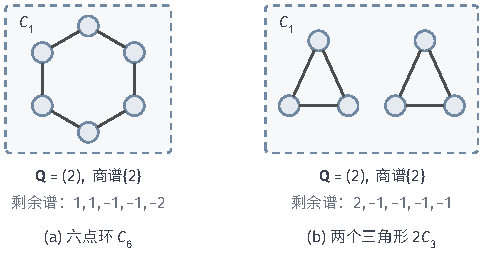
\includegraphics{figures/03-graphs/05-matrices-and-spectra/tikz/adjacency-c6-vs-2c3-quotient/figure.pdf}
  \caption{商谱相同而剩余谱不同的两张$6$点$2$正则图。在统一初色下，两图的公平划分都只有单一色类$C_1=V$（虚线框，$k=1$），商矩阵均为$\bm Q=(2)$，商谱均为$\{2\}$。(a) 六点环$C_6$在$\mathcal W^\perp$上的$5$个剩余特征值为$1,1,-1,-1,-2$。(b) 两个三角形$2C_3$在$\mathcal W^\perp$上的$5$个剩余特征值为$2,-1,-1,-1,-1$。}
  \label{fig:adjacency-c6-vs-2c3-quotient}
\end{BookInlineFigure}

最后，把$C_6$与$2C_3$的例子同第~\ref{sec:adjacency-cospectral-graphs}小节的五顶点同谱图$K_{1,4}$与$C_4\sqcup K_1$（图~\ref{fig:adjacency-cospectral-pair}）放在一起，就能看清颜色细化（公平划分）与完整邻接谱在区分非同构图时的互补关系。

一方面，商谱只是完整邻接谱在$\mathcal W$上的子集：像$C_6$与$2C_3$这样颜色细化完全无法区分（公平划分与商谱均相同）的两张正则图，仍有可能依靠$\mathcal W^\perp$上的剩余谱被完整邻接谱区分开。

另一方面，完整邻接谱也并不能涵盖颜色细化的全部信息：$K_{1,4}$与$C_4\sqcup K_1$拥有完全相同的完整邻接谱$\{2,0,0,0,-2\}$，但颜色细化在第一轮按顶点度分色时，就会把$K_{1,4}$拆成度为$4$和度为$1$的两个色类（大小$1+4$，商矩阵$\bigl(\begin{smallmatrix}0&4\\1&0\end{smallmatrix}\bigr)$），而把$C_4\sqcup K_1$拆成度为$2$和度为$0$的两个色类（大小$4+1$，商矩阵$\bigl(\begin{smallmatrix}2&0\\0&0\end{smallmatrix}\bigr)$），从而将这两张同谱图区分开。完整邻接谱与公平划分各自从特征值多重集和局部度传递层次刻画了图的结构。

\section{本章小结}
\label{sec:adjacency-matrix-summary}

邻接矩阵的$k$次幂在位置$(u,v)$记录从$u$到$v$的$k$步行走条数。对角元之和（迹）给出闭行走总数。实对称性保证迹等于特征值$k$次幂之和，这就是谱矩。

典型图的谱可以直接构造。完全图利用常向量与零和向量，完全二部图利用两侧对称，环利用周期边界的单位根，路径利用零端边界的正弦模式。笛卡儿积图的特征值等于各因子特征值之和。正则图的常向量特征值等于度，补图的谱由此换算。

谱本身具有结构性质。连通图的最大特征值是单根，有严格正的Perron向量。它夹在平均度和最大度之间，连通正则图中两端同时取等。删边或删正权顶点不增大谱半径。二部图的谱关于零对称，非二部图没有这种对称。

完整谱与图结构的关系体现在两个方面。一方面，谱记录了图的宏观代数特征：低阶谱矩确定边数和三角形数，极端特征值限制直径、独立数和色数。另一方面，谱丢失了同构信息：$K_{1,4}$和$C_4\sqcup K_1$有相同谱却不同构，不同来源的闭行走在求和后互相补偿。

更粗的商谱进一步缩减信息。等价划分把图缩成商矩阵，颜色细化给出最粗的等价划分。商谱保留了块间连接密度的框架，丢失了块内的微观差异——颜色细化分不出的两张图，完整谱仍可以不同。

下一章把邻接作用换成沿边差分再加权汇总，得到拉普拉斯矩阵。常值函数的沿边差分全为零，因此零空间直接揭示连通分量——恰好弥补邻接谱在这方面的缺失。


\chapter{拉普拉斯矩阵}
\label{chap:graph-laplacian-matrix}

沿用图~\ref{fig:incidence-running-example}中的四点五边图：四条外圈环边为$12,23,34,41$，另有一条对角边$13$。除特别说明外，五条边的权重均取$1$；一般推导考虑至少含一个顶点的有限无向无自环图，边权非负；涉及第二小特征值时另设$n\geq2$。

我们先用一个具体计算引入拉普拉斯矩阵。设顶点$1$的读数为$3$，它的三个邻居$2,3,4$的读数分别为$2,1,0$。将顶点$1$的本点读数分别减去三个邻居的读数，得到$3-2=1$、$3-1=2$、$3-0=3$，三项相加为$6$。这一运算汇总了本点读数相对于所有相邻顶点的偏离总和。

对全图每个顶点同时执行这一运算，就得到顶点空间上的对称线性算子——组合拉普拉斯矩阵$\bm L=\bm D-\bm W$。结合第~\ref{chap:graph-incidence-matrix}章的带符号关联矩阵$\bm B$，这一算子可分解为“沿边取差—乘边权—按顶点汇总”三步复合$\bm L=\bm B\bm C\bm B^\top$，其二次型$\bm x^\top\bm L\bm x=\sum_{\{i,j\}\in E}w_{i,j}(x_i-x_j)^2$直接给出全图各边读数差的加权平方和。

围绕这一核心矩阵，本章按照“矩阵定义—二次型—拉普拉斯谱—生成树计数—按度归一化”的脉络展开：第~\ref{sec:graph-laplacian}节建立加权度、度矩阵以及组合拉普拉斯矩阵$\bm L$的逐点定义与关联矩阵分解；第~\ref{sec:graph-laplacian-energy}节定义拉普拉斯二次型，证明$\bm L$的半正定性等基本性质，阐明二次型与图平滑性及割边权重的结构联系，并简介其在图分割与图信号去噪中的应用。

第~\ref{sec:graph-laplacian-eigenvalues}节研究$\bm L$的拉普拉斯谱，依次讨论特征值、零特征值与连通分量、特征值的上下界、加边单调性以及典型图族的显式谱。

第~\ref{sec:graph-matrix-tree}节将拉普拉斯矩阵的主余子式与除去一个零特征值后的其余特征值乘积应用于生成树计数，证明矩阵树定理、谱计数公式与Cayley公式。

第~\ref{sec:graph-normalized-laplacian}节针对度数不均图上的扩散与划分问题，引入度加权内积、对称归一化拉普拉斯$\mathcal L$与随机游走拉普拉斯$\bm L_{\mathrm{rw}}$，对比两种归一化算子并证明归一化拉普拉斯谱的性质。

\section{组合拉普拉斯}
\label{sec:graph-laplacian}

第~\ref{chap:graph-incidence-matrix}章的关联矩阵$\bm B$把顶点函数映射为沿边差分，又把边上的流量汇总到各顶点。如果将“沿边取差—乘以边权—按顶点汇总”三步复合起来，就得到顶点空间$\mathbb R^n$上的对称线性算子——组合拉普拉斯矩阵$\bm L$。本节依次介绍加权度与度矩阵、组合拉普拉斯矩阵的逐点定义以及它与关联矩阵的分解关系。

\subsection{加权度与度矩阵}
\label{sec:graph-weighted-adjacency}

沿用第~\ref{chap:graph-adjacency-matrix}章的记号。设有限无向无自环图$\mathcal G=(V,E)$有$n$个顶点、$m$条边，加权邻接矩阵$\bm W=(w_{i,j})\in\mathbb R^{n\times n}$在每对相邻顶点$(i,j)$处记录边权$w_{i,j}=w_{j,i}\geq 0$，无边处和对角线处均取零。

给定顶点函数$\bm x\in\mathbb R^n$，矩阵乘积$\bm W\bm x$的第$i$个分量把顶点$i$的所有邻居读数按对应边权加权求和：
\begin{equation}
  (\bm W\bm x)_i=\sum_{j=1}^n w_{i,j}\,x_j.
  \label{eq:graph-weighted-neighbor-sum}
\end{equation}
在图~\ref{fig:incidence-running-example}的四点五边单位权图上取读数$\bm x=(3,2,1,0)^\top$，第一行对顶点$1$的三个邻居$2,3,4$求和，得到$1\cdot2+1\cdot1+1\cdot0=3$；第二行只对顶点$2$的两个邻居$1$和$3$求和，得到$1\cdot3+1\cdot1=4$。如果把所有顶点的读数都取为常值$1$，顶点$1$的输出是$1+1+1=3$，而顶点$2$的输出是$1+1=2$。可见即使各点读数完全相同，$(\bm W\bm x)_i$的数值仍随顶点连接的总边权而不同。

将一个顶点的全部邻边权重相加，就得到该顶点的\term{加权度}（weighted degree），排成对角矩阵即得\emph{度矩阵}（degree matrix）：
\begin{equation}
  d_i=\sum_{j=1}^n w_{i,j}=(\bm W\bm 1)_i,\qquad
  \bm D=\operatorname{diag}(d_1,\ldots,d_n).
  \label{eq:graph-laplacian-weighted-degree}
\end{equation}
在单位权图中，$d_i$就是顶点$i$的邻居个数。若增大某条现有边的权重，只有该边两个端点的加权度随之增加，图的连接结构本身并不改变。由于所有边权非负，加权度$d_i=0$当且仅当顶点$i$关联的所有边权重全为零，即$i$是定义~\ref{def:positive-weight-support}中正权支撑$\mathcal G_+=(V,E_+)$的孤立顶点。

在四点五边算例中，顶点$1,3$各连接三个邻居，顶点$2,4$各连接两个邻居。当五条边均取单位权时，度向量为$\bm d=(3,2,3,2)^\top$；若仅把对角边$13$的权重改为$2$，则两端点$1$和$3$的加权度各增加$1$，度向量变为$(4,2,4,2)^\top$。除特别说明外，后文算例仍取全部边为单位权。

\subsection{组合拉普拉斯的定义}
\label{sec:graph-laplacian-matrix-form}

有了邻居加权和$\bm W\bm x$与度矩阵$\bm D$，就可以把“本点读数相对于各邻居读数的带权偏离总和”写成线性算子。对每条边$\{i,j\}$，用本点读数$x_i$减去邻居读数$x_j$，再乘上边权$w_{i,j}$；把顶点$i$所有邻边的带权差相加，就得到组合拉普拉斯在顶点$i$处的输出。

\begin{definition}[组合拉普拉斯矩阵]
\label{def:graph-combinatorial-laplacian}
设$\bm W$和$\bm D$分别为有限无向非负加权图的加权邻接矩阵和度矩阵。图的\term{组合拉普拉斯}（combinatorial Laplacian）矩阵$\bm L\in\mathbb R^{n\times n}$定义为
\begin{equation}
  (\bm L\bm x)_i=\sum_{j=1}^n w_{i,j}(x_i-x_j),\qquad
  \bm L=\bm D-\bm W.
  \label{eq:graph-combinatorial-laplacian}
\end{equation}
\end{definition}

将式~\eqref{eq:graph-combinatorial-laplacian}第一式按被减数与减数拆开：
\[
  (\bm L\bm x)_i
  =\sum_{j=1}^n w_{i,j}x_i - \sum_{j=1}^n w_{i,j}x_j
  =d_i x_i - (\bm W\bm x)_i.
\]
其中被减数部分$(\bm D\bm x)_i=d_i x_i$收集了本点读数的全部权重系数，减数部分$(\bm W\bm x)_i$则是式~\eqref{eq:graph-weighted-neighbor-sum}的邻居加权和，写成矩阵等式即为$\bm L=\bm D-\bm W$。

当$d_i>0$时，还可从邻域平均的角度理解这一输出。将$d_i$提取出来，式~\eqref{eq:graph-combinatorial-laplacian}可改写为
\[
  (\bm L\bm x)_i = d_i\left(x_i - \sum_{j=1}^n \frac{w_{i,j}}{d_i}x_j\right).
\]
括号内的求和是邻居读数按权重份额$w_{i,j}/d_i$（总和为$1$）计算的加权平均值，因此$(\bm L\bm x)_i$等于加权度$d_i$乘以本点读数高出邻居加权平均值的幅度。

定义~\ref{def:graph-combinatorial-laplacian}是按顶点逐行遍历邻居的写法；若改为按边逐条汇总，就能把$\bm L$与第~\ref{chap:graph-incidence-matrix}章的带符号关联矩阵$\bm B\in\mathbb R^{n\times m}$直接联系起来。固定每条边$e=\{i,j\}$的参考方向$i\to j$，关联矩阵的第$e$列为$\bm b_e=\bm e_i-\bm e_j$。将$\bm L$作用于顶点函数$\bm x$的过程可分解为先后衔接的三步：

第一步是沿边取差。左乘$\bm B^\top$将$n$维顶点函数$\bm x$映射为$m$维沿边差分向量$\bm B^\top\bm x$，其第$e$个分量为
\[
  (\bm B^\top\bm x)_e=\bm b_e^\top\bm x=x_i-x_j.
\]

第二步是按边乘权。左乘边权对角阵$\bm C=\operatorname{diag}(w_{e_1},\ldots,w_{e_m})$，将每条边的差值乘以该边的权重，得到带权边差向量$\bm C\bm B^\top\bm x$，其第$e$个分量为$w_e(x_i-x_j)$。

第三步是按顶点汇总。左乘$\bm B$把每条边的带权差送回它的两个端点：边$e$对应的单列项$w_e\bm b_e(\bm b_e^\top\bm x)$在尾端$i$处加上$w_e(x_i-x_j)$，在头端$j$处加上$-w_e(x_i-x_j)=w_e(x_j-x_i)$。将全部$m$条边的贡献叠加，即得组合拉普拉斯的关联矩阵分解：
\begin{equation}
  \bm L=\sum_{e\in E} w_e\bm b_e\bm b_e^\top
       =\bm B\bm C\bm B^\top.
  \label{eq:graph-laplacian-incidence-factorization}
\end{equation}

在式~\eqref{eq:graph-laplacian-incidence-factorization}的每一项秩一矩阵$w_e\bm b_e\bm b_e^\top$中，列向量$\bm b_e$出现两次。若反转边$e$的参考方向，$\bm b_e$变为$-\bm b_e$，两次负号相互抵消，故$\bm L$完全不依赖各边参考方向的选取。

图~\ref{fig:laplacian-readings-aggregation}在四点单位权图上展示了“沿边取差—乘边权—按顶点汇总”的三步过程。例如边$41$的参考方向为$4\to 1$，沿边差分为$x_4-x_1=0-3=-3$；汇总到头端顶点$1$时乘以$B_{1,41}=-1$得到$-(-3)=+3$，与边$12$送来的$+1$和边$13$送来的$+2$相加，给出$(\bm L\bm x)_1=6$。

\begin{BookInlineFigure}
  \centering
  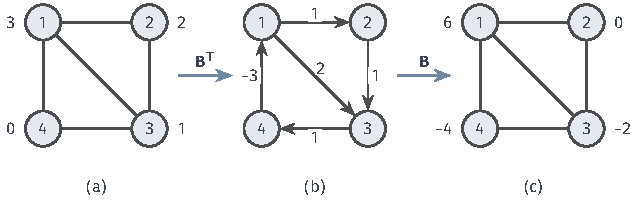
\includegraphics{figures/03-graphs/05-matrices-and-spectra/tikz/laplacian-readings-aggregation.pdf}
  \caption{四点单位权图上计算$\bm L\bm x$的三步分解。（a）顶点旁标注读数$\bm x=(3,2,1,0)^\top$。（b）箭头表示参考方向，边旁数字为沿边差分$\bm B^\top\bm x$（单位权下乘$\bm C$后不变）。（c）左乘$\bm B$汇总回各顶点的输出$\bm L\bm x=(6,0,-2,-4)^\top$。}
  \label{fig:laplacian-readings-aggregation}
\end{BookInlineFigure}

由分解式~\eqref{eq:graph-laplacian-incidence-factorization}立即可见：当所有顶点取同一常数$\bm x=c\bm 1$时，每条边两端读数相等，沿边差分$\bm B^\top(c\bm 1)=\bm 0$，从而$\bm L(c\bm 1)=\bm 0$。无论各顶点的加权度如何分布，全一常向量$\bm 1$始终属于$\bm L$的零空间。

在四点五边单位权算例中，将度向量$\bm d=(3,2,3,2)^\top$填入对角线，并在五条边对应的非对角位置各填$-1$，即得
\[
  \bm L=
  \begin{bmatrix}
  3&-1&-1&-1\\
  -1&2&-1&0\\
  -1&-1&3&-1\\
  -1&0&-1&2
  \end{bmatrix}.
\]
用单位脉冲$\bm e_1=(1,0,0,0)^\top$核对第一列：顶点$1$比三个邻居$2,3,4$各高出$1$，偏离总和为$3$；三个邻居$2,3,4$各自只有一个读数为$1$的邻居，偏离量均为$0-1=-1$，所得$(3,-1,-1,-1)^\top$恰好是$\bm L$的第一列。

\section{拉普拉斯二次型}
\label{sec:graph-laplacian-energy}

上一节给出了组合拉普拉斯矩阵$\bm L=\bm D-\bm W=\bm B\bm C\bm B^\top$及其对顶点函数$\bm x\in\mathbb R^n$的线性作用$\bm x\mapsto\bm L\bm x$。将线性输出$\bm L\bm x$与原向量$\bm x$作内积，就得到实对称矩阵$\bm L$所对应的二次型$\bm x^\top\bm L\bm x$。本节依次介绍拉普拉斯二次型的定义、半正定性等基本代数性质、它与图上顶点读数平滑性及子集割边权重的关系，最后简要介绍它在图分割与图信号处理中的应用。

\subsection{拉普拉斯二次型的定义}
\label{sec:graph-laplacian-quadratic-form}

在线性输出$(\bm L\bm x)_i=\sum_j w_{i,j}(x_i-x_j)$中，同一个顶点与不同邻居的一正一负差值会在求和时相互抵消。例如在三点单位权路径$1\!-\!2\!-\!3$上取$\bm x=(0,1,2)^\top$，中间顶点$2$与左邻$1$相差$+1$、与右邻$3$相差$-1$，相加得到$(\bm L\bm x)_2=0$，仅看该点输出看不出读数正在沿路径递增。

若改为考察二次型$\bm x^\top\bm L\bm x$，利用关联矩阵分解式~\eqref{eq:graph-laplacian-incidence-factorization}，可以把顶点空间上的内积$\bm x^\top(\bm L\bm x)$逐步转写到边空间上。记沿边差分向量为$\bm z=\bm B^\top\bm x\in\mathbb R^m$，其第$e$个分量（对应边$e=\{i,j\}$）为$z_e=x_i-x_j$，则
\[
  \begin{aligned}
    \bm x^\top\bm L\bm x
    &=\bm x^\top(\bm B\bm C\bm B^\top)\bm x\\
    &=(\bm B^\top\bm x)^\top\bm C(\bm B^\top\bm x)\\
    &=\bm z^\top\bm C\bm z\\
    &=\sum_{\{i,j\}\in E}w_{i,j}(x_i-x_j)^2.
  \end{aligned}
\]
若将关于无向边$\{i,j\}\in E$的求和改写为关于全体有序顶点对$(i,j)\in V\times V$的双重求和，每条无向边在$(i,j)$与$(j,i)$处各被计入一次，故须乘以因子$\frac12$。

\begin{definition}[拉普拉斯二次型与沿边变化能量]
\label{def:graph-dirichlet-energy}
设$\mathcal G=(V,E)$为有限无向非负加权图，$\bm L=\bm D-\bm W=\bm B\bm C\bm B^\top$为其组合拉普拉斯矩阵。对任意顶点函数$\bm x\in\mathbb R^n$，称
\begin{equation}
  \bm x^\top\bm L\bm x
  =\lVert\bm C^{1/2}\bm B^\top\bm x\rVert_2^2
  =\sum_{\{i,j\}\in E}w_{i,j}(x_i-x_j)^2
  =\frac12\sum_{i,j=1}^n w_{i,j}(x_i-x_j)^2
  \label{eq:graph-laplacian-energy}
\end{equation}
为$\bm x$的\emph{拉普拉斯二次型}（Laplacian quadratic form），也称为$\bm x$在图上的\term{沿边变化能量}（Dirichlet energy）。
\end{definition}

与逐点线性输出不同，式~\eqref{eq:graph-laplacian-energy}对每条边的两端差值$x_i-x_j$先平方再乘以边权$w_{i,j}$求和，因此不同边上的正负差值不再相互抵消。在刚才的三点路径上，$\bm x=(0,1,2)^\top$的二次型为$(0-1)^2+(1-2)^2=2$，真实反映了读数在两条边上的累积变化。

\subsection{拉普拉斯二次型的性质}
\label{sec:graph-laplacian-quadratic-properties}

由定义式~\eqref{eq:graph-laplacian-energy}中“加权平方和”的结构，可以直接导出组合拉普拉斯矩阵$\bm L$的半正定性以及二次型的平移不变性与边权可加性。

\begin{theorem}[拉普拉斯二次型的性质与半正定性]
\label{prop:graph-laplacian-quadratic-form}
设$\mathcal G=(V,E)$为有限无向非负加权图，组合拉普拉斯矩阵为$\bm L$。则：
\begin{enumerate}
  \item \emph{半正定性}：$\bm L$是实对称半正定矩阵，即对任意$\bm x\in\mathbb R^n$都有$\bm x^\top\bm L\bm x\geq 0$；且$\bm x^\top\bm L\bm x=0$当且仅当在每条正权边$\{i,j\}\in E_+$上都有$x_i=x_j$。
  \item \emph{常数平移不变性}：对任意$\bm x\in\mathbb R^n$和任意实数$c\in\mathbb R$，有
  \[
    (\bm x+c\bm 1)^\top\bm L(\bm x+c\bm 1)=\bm x^\top\bm L\bm x.
  \]
  \item \emph{关于边权的可加性与单调性}：若同一顶点集$V$上的两张非负加权图$\mathcal G_1,\mathcal G_2$按对应边权相加合成图$\mathcal G=\mathcal G_1+\mathcal G_2$，则对任意$\bm x\in\mathbb R^n$有
  \[
    \bm x^\top\bm L(\mathcal G)\bm x
    =\bm x^\top\bm L(\mathcal G_1)\bm x+\bm x^\top\bm L(\mathcal G_2)\bm x
    \geq\bm x^\top\bm L(\mathcal G_1)\bm x.
  \]
\end{enumerate}
\end{theorem}

\begin{proof}
（1）由$\bm W^\top=\bm W$和$\bm D^\top=\bm D$知$\bm L^\top=(\bm D-\bm W)^\top=\bm L$，故$\bm L$是实对称矩阵。在式~\eqref{eq:graph-laplacian-energy}中，由于每条边的权重$w_{i,j}\geq 0$且平方项$(x_i-x_j)^2\geq 0$，各项均非负，故$\bm x^\top\bm L\bm x\geq 0$，即$\bm L$半正定。非负项之和为零当且仅当每一项都为零；对于$w_{i,j}>0$的正权边$\{i,j\}\in E_+$，这等价于$(x_i-x_j)^2=0$，即$x_i=x_j$。

（2）将每个顶点的读数同时加上常数$c$后，任意一条边$\{i,j\}$两端的读数差为$(x_i+c)-(x_j+c)=x_i-x_j$，逐边差值完全不变，代入式~\eqref{eq:graph-laplacian-energy}即知二次型不变（这也与$\bm L\bm 1=\bm 0$一致）。

（3）当边权相加$w_{i,j}=w_{i,j}^{(1)}+w_{i,j}^{(2)}$时，由$\bm L=\sum_{e\in E}w_e\bm b_e\bm b_e^\top$对边权的线性性，有$\bm L(\mathcal G)=\bm L(\mathcal G_1)+\bm L(\mathcal G_2)$。左乘$\bm x^\top$、右乘$\bm x$即得二次型的可加性；再由$\bm x^\top\bm L(\mathcal G_2)\bm x\geq 0$立得不等式。
\end{proof}

\subsection{二次型与图结构}
\label{sec:graph-laplacian-cut-quadratic-form}

式~\eqref{eq:graph-laplacian-energy}将代数二次型$\bm x^\top\bm L\bm x$与图的拓扑连接紧密绑定在一起，主要体现在连续向量的沿边平滑度与离散子集的割边代价两个方面。

对于一般实向量$\bm x\in\mathbb R^n$，$\bm x^\top\bm L\bm x$度量了\emph{顶点函数沿图结构的平滑程度}。在求和式$\sum_{\{i,j\}\in E}w_{i,j}(x_i-x_j)^2$中，每一项都用边权$w_{i,j}$惩罚相邻顶点取值的不一致：如果图中相连的顶点（尤其是边权$w_{i,j}$较大的紧密连接顶点对）拥有相近的读数$x_i\approx x_j$，那么每条边上的$(x_i-x_j)^2$都很小，$\bm x^\top\bm L\bm x$就会非常小；反之，如果相邻顶点的读数剧烈反号或相差悬殊，$\bm x^\top\bm L\bm x$就会很大。

以四点五边单位权图为例，同样取长度为$2$的零和向量作比较。若取$\bm x=(1,1,-1,-1)^\top$，边$12$和边$34$两端读数相同（差为$0$），只有边$23,41,13$跨越正负号（差为$2$），二次型为$3\times 2^2=12$；若改为取$\bm x=(1,-1,1,-1)^\top$，四条外圈环边两端全部正负交替（差均为$2$），二次型增大为$4\times 2^2=16$。

当$\bm x=\bm 1_S$取为某个顶点子集$S\subseteq V$的$0$--$1$指示向量（在$i\in S$处取$1$，在$i\notin S$处取$0$）时，拉普拉斯二次型\emph{精确等于跨子集边界被切断的边的总权重（割边代价）}。对图中任意一条边$\{i,j\}\in E$，若两端点同在$S$内部或同在$V\setminus S$内部，则$\bm 1_S(i)=\bm 1_S(j)$，该边平方差为$0$；只有一端在$S$内、另一端在$V\setminus S$内的跨割边满足$|\bm 1_S(i)-\bm 1_S(j)|=1$，从而贡献其边权$w_{i,j}$：
\begin{equation}
  \bm 1_S^\top\bm L\bm 1_S
  =\sum_{\{i,j\}\in E}w_{i,j}(\bm 1_S(i)-\bm 1_S(j))^2
  =\sum_{i\in S,\,j\in V\setminus S}w_{i,j}
  =c(S,V\setminus S).
  \label{eq:graph-laplacian-cut-energy}
\end{equation}
同理，若用$\pm 1$指示向量$\bm s=2\bm 1_S-\bm 1$（在$S$内取$+1$，在$V\setminus S$内取$-1$）标记二分划分，则每条跨割边两端相差$2$、平方为$4$，从而$\bm s^\top\bm L\bm s=4\,c(S,V\setminus S)$。

图~\ref{fig:laplacian-edge-energy}在四点五边单位权图上展示了两个$0$--$1$指示向量的二次型。图~\ref{fig:laplacian-edge-energy}(a)取$S=\{1,3\}$的指示向量$\bm x=(1,0,1,0)^\top$，对角边$13$两端同在$S$内（差为$0$），四条外圈环边均跨越$S$与$\{2,4\}$（平方差各为$1$），故$\bm x^\top\bm L\bm x=4=c(\{1,3\},\{2,4\})$。图~\ref{fig:laplacian-edge-energy}(b)取单点集$S=\{1\}$的指示向量$\bm e_1=(1,0,0,0)^\top$，被切断的边恰好是与顶点$1$关联的三条边$12,41,13$，故$\bm e_1^\top\bm L\bm e_1=3=d_1$，这与对角元$L_{i,i}=\bm e_i^\top\bm L\bm e_i=d_i$完全一致。

\begin{BookInlineFigure}
  \centering
  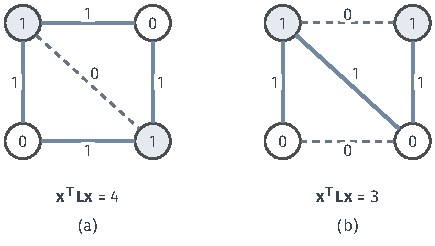
\includegraphics{figures/03-graphs/05-matrices-and-spectra/tikz/laplacian-edge-energy.pdf}
  \caption{四点单位权图上两个$0$--$1$指示向量的拉普拉斯二次型$\bm x^\top\bm L\bm x$。圆内为顶点读数，边旁为该边的平方差$(x_i-x_j)^2$。实线为跨割边（贡献$1$），虚线为同侧边（贡献$0$）。（a）$\bm x=\bm 1_{\{1,3\}}=(1,0,1,0)^\top$的二次型为$4$。（b）$\bm e_1=\bm 1_{\{1\}}=(1,0,0,0)^\top$的二次型为$3=d_1$。}
  \label{fig:laplacian-edge-energy}
\end{BookInlineFigure}

\subsection{在图问题中的应用}
\label{sec:graph-laplacian-quadratic-applications}

得益于“离散指示向量上等于割边代价、连续实向量上度量沿边平滑度”这一双重特性，拉普拉斯二次型在图算法与图数据分析中常作为核心目标函数或正则项出现。

第一类典型应用是\emph{图分割}（graph partitioning）。要把一张图切分为内部连接紧密、跨区连接稀疏的两个子集$S$与$V\setminus S$，就需要最小化跨子集的割边代价$c(S,V\setminus S)=\bm 1_S^\top\bm L\bm 1_S$，同时在子集大小$|S|$或连接体积上施加平衡约束，防止切出孤立小碎片。直接搜索最优离散子集是组合难问题；将离散指示向量松弛为满足正交与长度约束的连续实向量$\bm x\in\mathbb R^n$并最小化二次型$\bm x^\top\bm L\bm x$，离散割问题就转化为对称矩阵的瑞利商极值与特征向量计算问题，这也是第~\ref{chap:spectral-partition}章谱划分方法的出发点。

第二类典型应用是\emph{图信号处理中的去噪与平滑}（graph signal denoising and smoothing）。在传感器网络、社交网络或三维网格上，每个顶点带有一个观测读数$y_i$，排成观测向量$\bm y\in\mathbb R^n$。在采用图平滑先验的模型中，假设待恢复信号在相连顶点之间变化较小，而观测扰动会增加沿边差异；这一假设须与具体数据相符。将拉普拉斯二次型作为图平滑正则项加入最小二乘拟合，可构造如下去噪目标：
\begin{equation}
  \min_{\bm x\in\mathbb R^n}\Bigl\{\lVert\bm x-\bm y\rVert_2^2 + \gamma\,\bm x^\top\bm L\bm x\Bigr\}\qquad(\gamma>0),
  \label{eq:graph-laplacian-denoising}
\end{equation}
其中第一项要求恢复信号$\bm x$贴近观测$\bm y$，第二项以权重$\gamma$惩罚相连顶点之间的数值跳变。

由于$\bm L$半正定，式~\eqref{eq:graph-laplacian-denoising}的目标函数关于$\bm x$严格凸。对$\bm x$求梯度并令其为零，得到线性方程组
\[
  (\bm I+\gamma\bm L)\bm x=\bm y,\qquad
  \bm x=(\bm I+\gamma\bm L)^{-1}\bm y.
\]
该解在拟合观测与降低沿边变化之间作折中；若真实信号含有沿边突变，平滑正则化也可能引入偏差。类似地，若仅在部分边界顶点上已知标签读数，而在其余未知顶点上直接最小化沿边变化能量$\bm x^\top\bm L\bm x$，则得到图上的谐波插值与半监督标签传播；每个正权连通分量都含已知边界顶点时，未知读数唯一确定，其物理对应正是第~\ref{chap:graph-electrical-networks}章电网络中的最小能量原理。

\section{拉普拉斯特征值}
\label{sec:graph-laplacian-eigenvalues}

把一组顶点读数全部乘$2$，每条边的差也乘$2$，平方之后能量变成$4$倍。要比较两组读数在图上变化的方式——而不是单纯因为数值放大而显得能量更高——就需要先把它们缩放到相同的长度。特征向量给出了一组这样的标准方向，特征值告诉我们每个标准方向上的沿边能量。

\subsection{特征向量的变化尺度}
\label{sec:graph-laplacian-frequency}

$\bm L$是实对称矩阵，因此可以取一组标准正交特征向量$\bm u_1,\ldots,\bm u_n$，对应的特征值按$0=\lambda_1\leq\lambda_2\leq\cdots\leq\lambda_n$排列。实对称矩阵的正交谱分解可参考\BookChapterRef{chap:eigen-spectral-decomposition}{卷二"谱分解"章}。

任意顶点读数$\bm x$可以在这组特征基下表示。将$\bm x$投影到每个特征方向上，得到坐标$a_i=\bm u_i^\top\bm x$。这些坐标还原为顶点读数就是
\[
  \bm x=\sum_{i=1}^n a_i\bm u_i.
\]

作用一次拉普拉斯矩阵后，每个方向的坐标从$a_i$变成$\lambda_i a_i$：
\[
  \bm L\bm x=\sum_{i=1}^n\lambda_i a_i\bm u_i.
\]

现在用输入$\bm x$与输出$\bm L\bm x$做内积。由于特征向量两两正交，不同方向的交叉项为零，只有同一方向的坐标相乘。第$i$个方向贡献$a_i\cdot\lambda_i a_i=\lambda_i a_i^2$。类似地，$\bm x$与自身的内积给出各坐标平方之和。这就给出
\begin{equation}
  \bm x^\top\bm L\bm x
  =\sum_{i=1}^n\lambda_i a_i^2,\qquad
  \lVert\bm x\rVert_2^2=\sum_{i=1}^n a_i^2.
  \label{eq:graph-laplacian-spectral-energy}
\end{equation}

当$\bm x$恰好等于某个特征向量$\bm u_i$时，只有第$i$个坐标为$1$，其余全为$0$。此时长度为$1$，能量恰好等于$\lambda_i$。零特征值对应的方向在各连通分量内为常值，沿边没有变化。较小的正特征值对应整图上加权平方差之和较小的读数模式——但这是全图加权累计的结果，并不意味着每条边上的差都比其他方向小。

下面在四点图上逐个核验。先取
\[
  \bm x=(0,1,0,-1)^\top.
\]
顶点$1$的三个邻居$2,3,4$读数分别为$1,0,-1$，差值为$-1,0,1$，加起来为$0$。类似地，顶点$3$的输出也为$0$。顶点$2$的两个邻居$1$和$3$都是$0$，差值都等于自己，输出$2$。顶点$4$的两个邻居也都是$0$，输出$-2$。因此$\bm L\bm x=(0,2,0,-2)^\top=2\bm x$，这是特征值$2$的方向。

将此向量归一化为$\bm x/\sqrt2=(0,1/\sqrt2,0,-1/\sqrt2)^\top$。四条环边中，$12$和$41$的差平方为$1/2$，$23$和$34$也是$1/2$，共贡献$4\cdot(1/2)=2$。对角边$13$两端都是$0$，没有贡献。单位向量的总能量为$2$，确实等于特征值。

换成$\bm x=(1,0,-1,0)^\top$。顶点$1$的两个环邻居$2$和$4$各差$1$，对角邻居$3$差$2$，总和$1+2+1=4$。顶点$3$对称地得到$-4$。顶点$2$和$4$的两个邻居一正一负，恰好相消。因此$\bm L\bm x=(4,0,-4,0)^\top=4\bm x$，特征值为$4$。

最后取$\bm x=(1,-1,1,-1)^\top$。四条环边每对相邻顶点取值相差$2$，差平方为$4$。对角边$13$两端都是$1$，差为零。每个顶点的两个环邻居各贡献$2$，对角邻居（如果有的话）贡献$0$或$2$。以顶点$1$为例，邻居$2,3,4$的差值为$2,-2,2$，之和为$4\cdot1$，于是$\bm L\bm x=4\bm x$，特征值同样为$4$。

这三个非零特征方向加上常向量$(1,1,1,1)^\top$，构成四维空间的一组正交基。四点算例的完整拉普拉斯谱是$0,2,4,4$。特征值$4$出现两次，对应的两个特征向量$(1,0,-1,0)^\top$和$(1,-1,1,-1)^\top$描绘了不同的变化方式，但单位长度下的总能量相同。

图~\ref{fig:laplacian-four-modes}把四个单位特征向量画在同一张图上。比较后面两个方向：$(1,0,-1,0)^\top$在对角边上两端读数不同，$(1,-1,1,-1)^\top$在对角边上两端相同。但加上四条环边的贡献后，两者的总能量都等于$4$。

\begin{BookInlineFigure}
  \centering
  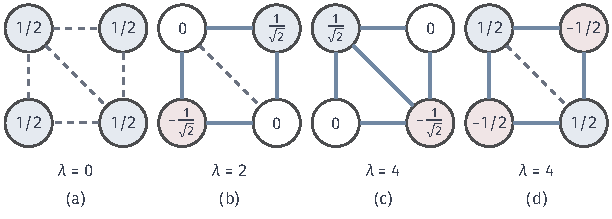
\includegraphics{figures/03-graphs/05-matrices-and-spectra/tikz/laplacian-four-modes.pdf}
  \caption{四点单位权图的四个单位特征向量。圆内为该点的坐标，浅蓝、浅红和白色分别表示正、负和零。两端读数不同的边画成实线，读数相等的边画成虚线。每幅图下的特征值就是沿边变化能量。}
  \label{fig:laplacian-four-modes}
\end{BookInlineFigure}

\subsection{特征值估计}
\label{sec:graph-laplacian-eigenvalue-bounds}

即使暂时没有求出全部特征向量，也能从度的信息估计特征值的范围。此外，在固定顶点集上加边后，各特征值只能不减。

先看上界。对单条边$\{i,j\}$，差的平方可以用两端读数各自的平方控制：
\[
  (x_i-x_j)^2\leq 2x_i^2+2x_j^2.
\]
将每条边的这个不等式乘上边权后求和。顶点$i$的$x_i^2$在它的每条邻边中都出现一次，这些边的权重加起来就是$d_i$。因此$x_i^2$的总系数为$2d_i$，从而
\[
  0\leq \bm x^\top\bm L\bm x
  \leq 2\sum_{i=1}^n d_ix_i^2
  \leq 2d_{\max}\lVert\bm x\rVert_2^2,
\]
其中$d_{\max}=\max_i d_i$。令$\bm x$取各单位特征向量，得到
\begin{equation}
  0\leq\lambda_i\leq 2d_{\max},\qquad i=1,\ldots,n.
  \label{eq:graph-laplacian-spectrum-bound}
\end{equation}
最大度给出了所有特征值的统一上界。

接下来考虑加边的影响。在固定的顶点集上增加一条权重为$a\geq0$的新边$e$，拉普拉斯矩阵从$\bm L$变为
\[
  \bm L'=\bm L+a\bm b_e\bm b_e^\top.
\]
新增项$a\bm b_e\bm b_e^\top$是半正定的，因此对任何向量$\bm x$，新图的二次型$\bm x^\top\bm L'\bm x$至少不小于旧图的$\bm x^\top\bm L\bm x$。

要把这个逐向量的比较转化为逐特征值的比较，需要用到 Courant--Fischer 刻画：第$i$个最小特征值等于"先选$i$维子空间，在子空间中求最大的单位能量，再在所有$i$维子空间中取最小值"。可参考\BookChapterRef{chap:condition-and-spectral-perturbation}{卷二"条件数与谱扰动"章}。

固定任何一个$i$维子空间$U$。旧图中在$U$内达到最大单位能量的向量放进新图，能量只会增加或保持，所以新图在$U$内的最大值不会更小。这对每个$U$都成立。在所有$U$中取最小值时，新图的最小值也不会更小。因此
\begin{equation}
  \lambda_i(\bm L')\geq\lambda_i(\bm L),\qquad i=1,\ldots,n.
  \label{eq:graph-laplacian-edge-monotonicity}
\end{equation}
这个比较使用同一个顶点集上的向量空间。删去一个顶点时，向量空间的维数和度都会改变，不能直接套用这个结论。

用四点图来验证。单位权四点环的谱是$0,2,2,4$（下面会给出环图的谱公式）。加入对角边$13$后变为$0,2,4,4$。观察方向$(1,0,-1,0)^\top$，它在新增边上两端读数不同，加入该边后沿边能量增加，这个方向原来对应特征值$2$，现在上升到$4$。另一方向$(0,1,0,-1)^\top$在新增边上两端相等，不受影响，仍对应$2$。

\subsection{典型图的拉普拉斯谱}
\label{sec:graph-typical-laplacian-spectra}

对几类常见图，可以利用它们的结构直接写出谱。正则图的拉普拉斯谱与邻接谱之间有简单的标量关系。

在简单无权的$d$正则图上，每个顶点的度都为$d$，所以$\bm D=d\bm I$。设$\bm x$是邻接矩阵$\bm A$的特征向量，对应特征值$\alpha$。拉普拉斯作用于$\bm x$时，
\[
  \bm L\bm x=(d\bm I-\bm A)\bm x=d\bm x-\alpha\bm x=(d-\alpha)\bm x.
\]
特征向量保持不变，邻接特征值$\alpha$变成了拉普拉斯特征值$d-\alpha$。如果各点度不同，$\bm D$不是标量矩阵，就不能用这种简单的平移换算。

利用这个关系，可以直接把上一章算出的邻接谱转成拉普拉斯谱。

\begin{theorem}[典型图的拉普拉斯谱]
\label{prop:graph-typical-laplacian-spectra}
\leavevmode
\begin{enumerate}
  \item 完全图$K_n$：$0$（重数$1$），$n$（重数$n-1$）。
  \item 环$C_n$（$n\ge3$）：$\lambda_k=2-2\cos(2\pi k/n)$，$k=0,\ldots,n-1$。
  \item 路径$P_n$（$n\ge2$）：$\lambda_k=2-2\cos(k\pi/n)$，$k=0,\ldots,n-1$。
  \item 星$K_{1,n-1}$（$n\ge2$）：$0$（重数$1$），$1$（重数$n-2$），$n$（重数$1$）。
\end{enumerate}
\end{theorem}

\paragraph{完全图}

对完全图$K_n$，邻接谱为$n-1$（重数$1$）和$-1$（重数$n-1$），度$d=n-1$，拉普拉斯谱为$0$（重数$1$）和$n$（重数$n-1$）。

\paragraph{环}

对环图$C_n$（$n\geq3$），邻接特征值为$2\cos(2\pi k/n)$，度$d=2$，拉普拉斯特征值为
\begin{equation}
  \lambda_k^{(C)}=2-2\cos(2\pi k/n),\qquad k=0,\ldots,n-1.
  \label{eq:graph-cycle-laplacian-spectrum}
\end{equation}
$k$是模态编号，写出的顺序不一定是特征值的升序。取$n=4$得到$0,2,4,2$，排序后为$0,2,2,4$，与四点环未加对角线时的谱一致。

\paragraph{路径}

对路径$P_n$，因为端点只有一个邻居。内部顶点$i$的拉普拉斯输出是$2x_i-x_{i-1}-x_{i+1}$。端点$1$只有右邻点$2$，输出是$x_1-x_2$。

为了统一处理端点和内部顶点，我们在左端外添一个辅助坐标$x_0=x_1$。此时
\[
  2x_1-x_0-x_2=2x_1-x_1-x_2=x_1-x_2,
\]
与端点的真实输出一致。等值的辅助坐标没有引入新的沿边差异。右端同样用$x_{n+1}=x_n$。

接下来找满足$x_{i-1}+x_{i+1}=\lambda x_i$的模式。尝试$x_i=\cos\bigl((i-\tfrac12)\theta\bigr)$，其中$\theta$是相邻读数的相位差。利用三角和差公式可得$x_{i-1}+x_{i+1}=2\cos\theta\cdot x_i$，因此内部顶点上的特征值为$2-2\cos\theta$。

左端的辅助条件自动满足：$\cos(-\theta/2)=\cos(\theta/2)$，余弦的偶性保证了$x_0=x_1$。右端的条件要求
\[
  x_{n+1}-x_n=-2\sin(n\theta)\sin(\theta/2)=0.
\]
取$\theta=k\pi/n$，$k=0,\ldots,n-1$，每个角度给出一个非零向量。$n$个不同的特征值为
\begin{equation}
  \lambda_k^{(P)}=2-2\cos(k\pi/n),\qquad k=0,\ldots,n-1.
  \label{eq:graph-path-laplacian-spectrum}
\end{equation}
其中半格偏移$\tfrac12$对应两端保持相同读数的边界条件，这与邻接矩阵路径公式所用的两端为零条件不同。

\paragraph{星图}

对星图$K_{1,n-1}$（$n\geq2$），设中心读数为零，各叶读数之和也为零。每片叶只与中心相连，输出等于自己的读数减去中心读数，即等于自己。中心读取所有叶的差值之和，由于叶总和为零，输出也为零。这给出维数$n-2$、特征值为$1$的子空间。

剩下两个方向可以取常向量（特征值$0$）和"中心为$n-1$、各叶为$-1$"的向量。后者在每条边上相差$n$，中心的邻居和为$(n-1)\cdot(-1)$，输出为$(n-1)(n-1-(- 1))=n(n-1)$。等等，这里更直接地算：各点的$\bm L$作用下，中心输出$d_{\text{center}}\cdot(n-1)-\sum_{\text{leaves}}(-1)=(n-1)(n-1)+(n-1)=n(n-1)$，而每片叶输出$1\cdot(-1-(n-1))=-n$。因此$\bm L\bm x=n\bm x$，特征值为$n$。四顶点星图的谱为$0,1,1,4$。虽然和四点路径一样有四个顶点三条边，两者的拉普拉斯谱完全不同。

\paragraph{补图}

最后看补图的谱换算。对简单无权图$\mathcal G$，它与补图$\overline{\mathcal G}$的边合在一起构成完全图，且没有重复。因此
\begin{equation}
  \bm L(\overline{\mathcal G})
  =\bm L(K_n)-\bm L(\mathcal G)
  =n\bm I-\bm1\bm1^\top-\bm L(\mathcal G).
  \label{eq:graph-complement-laplacian}
\end{equation}
常向量$\bm1$对两张图都是零方向。沿与常向量正交的原图特征向量$\bm u_i$（$i\geq2$），$\bm1\bm1^\top\bm u_i=\bm0$，因此补图的特征值变成$n-\lambda_i$。如果原图恰好有某个特征值等于$n$，补图在该方向上的特征值为零，对应一个额外的零方向——由定理~\ref{thm:graph-laplacian-components}可知，补图多了一个连通分量。

\section{拉普拉斯谱与生成树}
\label{sec:graph-matrix-tree}

第~\ref{sec:graph-laplacian-eigenvalues}节利用拉普拉斯矩阵的零特征值重数刻画了图的连通分量个数：正权支撑连通（即图中至少存在一棵正权生成树）当且仅当$\lambda_2>0$。本节进一步展示，拉普拉斯矩阵的主余子式以及除去一个零特征值后的$n-1$个特征值$\lambda_2,\ldots,\lambda_n$的乘积，能够精确数出一张图共有多少棵不同的生成树（在加权图中，给出所有生成树的边权乘积之和）。

在四点五边算例中，同样是从五条边中选出三条边，选$\{12,23,34\}$得到一条经过全部四个顶点的无环路径（是生成树），而选$\{12,23,13\}$则把三条边全用在三角形上、遗漏了顶点$4$（不是生成树，见图~\ref{fig:laplacian-tree-minors}）。要理解拉普拉斯矩阵为何能自动筛除所有含环边集、只保留生成树，我们按四个步骤推进：先分析约化关联矩阵的$(n-1)$阶子式如何区分生成树与含环边集，再结合 Cauchy--Binet 公式证明用主余子式计数生成树的矩阵树定理，接着通过特征多项式建立生成树计数的拉普拉斯谱公式，最后代入完全图的拉普拉斯谱导出经典的 Cayley 公式。

\subsection{生成树的关联子式}
\label{sec:graph-tree-incidence-minors}

固定一个顶点$r$作为根，从关联矩阵$\bm B$中删去第$r$行，得到$(n-1)\times m$的约化关联矩阵$\overline{\bm B}$。它仍保留全部$m$条边的列。然后按边序选择$n-1$条边组成集合$S$，只取这些边对应的列，得到$(n-1)\times(n-1)$的方阵$\overline{\bm B}_{:,S}$。

为什么可以删去根的那一行？因为$\bm B$的任一条边的列在两个端点分别取$+1$和$-1$，其余为$0$，所以$\bm B$的各行相加为零向量。一旦其余$n-1$行确定了，根行的值也由零和条件唯一确定。删去根行不会丢失信息。

\begin{lemma}[生成树的关联子式]
\label{lem:graph-tree-incidence-minors}
若$S$构成生成树，则$\det(\overline{\bm B}_{:,S})\in\{1,-1\}$。其他含$n-1$条边的集合$S$都使该行列式为零。
\end{lemma}

\begin{proof}
先处理$S$含环的情形。沿环选定一个行走方向，对每条环边，如果行走方向与记录方向一致就取原列，否则取负列。调整后，每列把环的上一步端点标为$+1$、下一步端点标为$-1$。

环上的任何一个顶点都在两条环边上出现：从进入的边收到$-1$，从离开的边收到$+1$，两者抵消为零。把调整后的列全部加起来，得到零向量。删去根行后仍然是零。这说明列之间有线性关系，行列式为零。

再处理$S$不含环的情形。$n$个顶点和$n-1$条无环边构成一个森林。设森林有$c$个连通分量，其中每棵树的顶点数比边数多一，因此总共有$n-c$条边。我们选了$n-1$条边，所以$c=1$，这组边构成一棵生成树。

对生成树，我们用递归计算它的关联子式。树中至少有两个顶点，就可以找到一个不是根的叶顶点。叶在生成树中只连一条边，因此$\overline{\bm B}_{:,S}$中对应的行只有一个非零条目，值为$+1$或$-1$。

沿这一行展开行列式，去掉叶所在的行和叶边所在的列，剩余矩阵是较小的树删去根行后的关联矩阵。每次展开只乘一个$\pm1$的因子。反复删去非根叶，最后只剩根，而根行在开始时已经删去，此时是一个空矩阵，行列式约定为$1$。逐层回乘，原行列式的绝对值为$1$。
\end{proof}

在四点算例中删去第$4$行。取边集$\{12,23,34\}$得到
\[
  \overline{\bm B}_{:,\{12,23,34\}}=
  \begin{bmatrix}
  1&0&0\\
  -1&1&0\\
  0&-1&1
  \end{bmatrix}.
\]
这是对角线全为$1$的下三角矩阵，行列式为$1$。改选$\{12,23,13\}$，由于这三条边构成三角形$1\!-\!2\!-\!3$，环的线性关系使行列式为零。后一组虽然也是三条边，却遗漏了顶点$4$。

图~\ref{fig:laplacian-tree-minors}把两种选法并排展示。左图中的边$34$经过根顶点$4$，但它的列仍然保留——删去的只是根对应的行，不影响边的列。

\begin{BookInlineFigure}
  \centering
  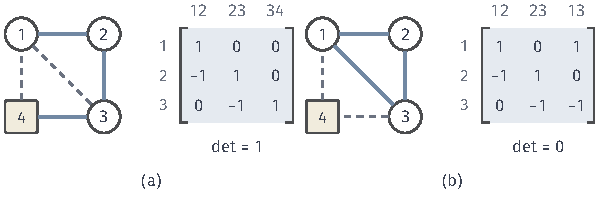
\includegraphics{figures/03-graphs/05-matrices-and-spectra/tikz/laplacian-tree-minors.pdf}
  \caption{固定根$4$后对照两组边的关联子式。方框标出根，它没有对应的矩阵行。实线表示选中的边，同时给出矩阵的列标。（a）生成树的子式行列式为一。（b）三角形的子式前两列相加等于第三列。}
  \label{fig:laplacian-tree-minors}
\end{BookInlineFigure}

\subsection{生成树的代数余子式计数}
\label{sec:graph-matrix-tree-proof}

现在把约化关联子式的判别性质与\BookChapterRef{chap:linear-operations}{卷二“向量、矩阵与张量的运算”章}的 Cauchy--Binet 公式结合起来，导出用拉普拉斯矩阵的代数余子式计数生成树的矩阵树定理。

从组合拉普拉斯矩阵$\bm L$中删去第$r$行和第$r$列，得到$(n-1)\times(n-1)$主子矩阵$\overline{\bm L}=\bm L^{(r,r)}$，其行列式$\det\overline{\bm L}=(-1)^{r+r}\det\bm L^{(r,r)}$正是对角位置$(r,r)$处的代数余子式$C_{r,r}$。

由关联分解式~\eqref{eq:graph-laplacian-incidence-factorization}，$\overline{\bm L}$的每个条目为
\[
  \overline L_{i,j}=\sum_{e\in E} B_{i,e}\,w_e\,B_{j,e},
\]
其中$i,j$遍历除$r$以外的$n-1$个顶点，求和仍遍及全部$m$条边。因此可以用$(n-1)\times m$约化关联矩阵$\overline{\bm B}$写成
\[
  \overline{\bm L}=\overline{\bm B}\,\bm C\,\overline{\bm B}^\top.
\]

进一步令$\bm M=\overline{\bm B}\bm C^{1/2}\in\mathbb R^{(n-1)\times m}$，使$\bm M$的每列为原来的约化关联列乘以该边权重的平方根$\sqrt{w_e}$。于是主子矩阵分解为
\[
  \overline{\bm L}=\bm M\bm M^\top,
\]
这正是 Cauchy--Binet 公式适用的矩形矩阵乘积形式。

\begin{theorem}[矩阵树定理]
\label{thm:graph-matrix-tree}
对有限无向非负权图，设$\mathcal T$为图的所有生成树的集合。则组合拉普拉斯矩阵$\bm L$在任意位置$(i,j)$处的代数余子式$C_{i,j}=(-1)^{i+j}\det\bm L^{(i,j)}$（特别地，删去任一顶点$r$的第$r$行与第$r$列所得的主余子式$\det\overline{\bm L}$）全部相等，且\term{矩阵树定理}（matrix-tree theorem）给出
\begin{equation}
  \det \overline{\bm L}=(-1)^{i+j}\det\bm L^{(i,j)}=\sum_{T\in\mathcal T}\prod_{e\in T}w_e.
  \label{eq:graph-matrix-tree}
\end{equation}
单位权时每棵生成树贡献$1$，该代数余子式就是生成树的数目。
\end{theorem}

\begin{proof}
第一步，对$(n-1)\times m$矩阵$\bm M$与$m\times(n-1)$矩阵$\bm M^\top$的乘积$\overline{\bm L}=\bm M\bm M^\top$应用 Cauchy--Binet 公式（参见\BookChapterRef{chap:linear-operations}{卷二“向量、矩阵与张量的运算”章}）。每次从$m$列中选出$n-1$个列指标（即选出一个$n-1$元边集$S\subseteq E$），由于$(\bm M^\top)_{S,:}=(\bm M_{:,S})^\top$，对应行和对应列组成的两个$(n-1)$阶子方阵互为转置、行列式相等，故
\[
  \det\overline{\bm L}
  =\sum_{\substack{S\subseteq E\\ |S|=n-1}}\det(\bm M_{:,S})\det\bigl((\bm M^\top)_{S,:}\bigr)
  =\sum_{\substack{S\subseteq E\\ |S|=n-1}}\det(\bm M_{:,S})^2.
\]

第二步，提取每条边的权重因子。$\bm M$的第$e$列是$\overline{\bm B}$的第$e$列乘以$\sqrt{w_e}$。取出$S$中各列后，由行列式对各列的齐次性，每列各提出一个$\sqrt{w_e}$因子，平方后变成$w_e$，因此
\[
  \det(\bm M_{:,S})^2=\det(\overline{\bm B}_{:,S})^2\prod_{e\in S}w_e.
\]

第三步，代入关联子式的判别结果。由引理~\ref{lem:graph-tree-incidence-minors}，如果$S$构成生成树，关联子式$\det(\overline{\bm B}_{:,S})$为$\pm1$，平方为$1$，该项贡献恰好是这棵生成树各边权重的乘积$\prod_{e\in S}w_e$；如果$S$不是生成树，关联子式为零，该项贡献为零。把所有非零项相加，即得对角位置的主余子式公式$\det\overline{\bm L}=\sum_{T\in\mathcal T}\prod_{e\in T}w_e$。

第四步，证明任意非对角位置$(i,j)$（$i\neq j$）的代数余子式$C_{i,j}=(-1)^{i+j}\det\bm L^{(i,j)}$也等于$\det\bm L^{(i,i)}$。在删去第$i$行与第$j$列所得的$(n-1)$阶子矩阵$\bm L^{(i,j)}$中，原矩阵的第$i$列保留了下来；将$\bm L^{(i,j)}$中除原第$i$列以外的其余$n-2$列全部加到原第$i$列上，行列式不变。由于$\bm L$的每一行元素之和为零（$\bm L\bm 1=\bm 0$），相加后原第$i$列在每一行上的新元素恰好等于$-\bm L^{(i,i)}$中原编号为$j$的列的元素。

最后，通过$|i-j|-1$次相邻列交换，把这一列移到原第$j$列在$\bm L^{(i,i)}$中的位置。列变号与列交换带来的总符号因子为$-(-1)^{|i-j|-1}=(-1)^{i+j}$，与代数余子式定义中的$(-1)^{i+j}$相乘恰好为$+1$，从而$(-1)^{i+j}\det\bm L^{(i,j)}=\det\bm L^{(i,i)}$。
\end{proof}

由于树权总和不涉及任何特定根，删去不同顶点的行列后得到的主余子式全都相等。含零权边的树在乘积中贡献为零；若正权支撑不连通，所有生成树至少包含一条零权边，权积全为零，代数余子式也为零。

下面在四点五边单位权算例上核对。删去顶点$3$对应的行和列，得到$3\times 3$约化矩阵
\[
  \overline{\bm L}=
  \begin{bmatrix}
  3&-1&-1\\
  -1&2&0\\
  -1&0&2
  \end{bmatrix}.
\]
沿第一行展开行列式：
\[
  \begin{aligned}
    \det\overline{\bm L}
    &=3\cdot\det\begin{bmatrix}2&0\\0&2\end{bmatrix}
      -(-1)\cdot\det\begin{bmatrix}-1&0\\-1&2\end{bmatrix}
      +(-1)\cdot\det\begin{bmatrix}-1&2\\-1&0\end{bmatrix}\\
    &=3\times 4 + 1\times(-2) - 1\times 2 = 12-2-2=8.
  \end{aligned}
\]

从组合计数看，五条边任选三条共有$\binom53=10$组。其中两个三角形$\{12,23,13\}$与$\{13,34,41\}$各自成环，贡献为零；其余$8$组各构成一棵生成树，单位权下各贡献$1$，总数为$8$。

若将对角边$13$的权重改为$2$，生成树的集合本身不变，但每棵包含边$13$的生成树权积变为$2$。含边$13$的生成树还需将顶点$2$和$4$分别接入$\{1,3\}$：顶点$2$可选边$12$或$23$（$2$种），顶点$4$可选边$34$或$41$（$2$种），共$2\times 2=4$棵。这$4$棵树各贡献$2$，其余$4$棵不含边$13$的树各贡献$1$，加权生成树总和变为$4\times 2+4\times 1=12$。

\subsection{生成树的拉普拉斯谱公式}
\label{sec:graph-tree-counting-formulas}

矩阵树定理把生成树权重总和表示为删去任一顶点行列所得的主余子式$\det\overline{\bm L}$。将全部$n$个顶点的主余子式汇总到$\bm L$的特征多项式一次项系数中，就可以直接用拉普拉斯矩阵的其余$n-1$个特征值$\lambda_2,\ldots,\lambda_n$表达生成树权重总和。

\begin{theorem}[生成树计数的拉普拉斯谱公式]
\label{cor:graph-tree-count-spectrum}
设$n\geq 2$，有限无向非负加权图的组合拉普拉斯特征值按升序排列为$0=\lambda_1\leq\lambda_2\leq\cdots\leq\lambda_n$。则图的生成树权重总和满足
\begin{equation}
  \sum_{T\in\mathcal T}\prod_{e\in T}w_e
  =\frac1n\prod_{i=2}^n\lambda_i.
  \label{eq:graph-tree-count-from-spectrum}
\end{equation}
\end{theorem}

\begin{proof}
第一步，从特征值展开计算$\det(t\bm I+\bm L)$中$t$的一次项系数。在$\bm L$的正交特征基下，$t\bm I+\bm L$的特征值为$t+\lambda_1,\ldots,t+\lambda_n$；因$\lambda_1=0$，有
\[
  \det(t\bm I+\bm L)=t\prod_{i=2}^n(t+\lambda_i).
\]
将其按$t$的幂展开，$t$的一次项系数为$\prod_{i=2}^n\lambda_i$。

第二步，从行列式按列的多线性计算同一系数。将$\det(t\bm I+\bm L)$的第$r$列写成$t\bm e_r + \bm L_{:,r}$；展开式中含$t$的一次项恰好来自“在某一列$r$选取$t\bm e_r$、在其余$n-1$列选取$\bm L$的原列”的所有组合。对固定的$r\in\{1,\ldots,n\}$，将第$r$列替换为$t\bm e_r$后沿第$r$列作拉普拉斯展开，所得$t$的系数正是删去$\bm L$的第$r$行与第$r$列后的主余子式$\det\overline{\bm L}^{(r)}$。

第三步，应用矩阵树定理求并比较系数。由定理~\ref{thm:graph-matrix-tree}，每个顶点$r$的主余子式均等于$\sum_{T\in\mathcal T}\prod_{e\in T}w_e$。对$r=1,\ldots,n$求和，可知$\det(t\bm I+\bm L)$中$t$的一次项系数又等于$n\sum_{T\in\mathcal T}\prod_{e\in T}w_e$。比较两种展开的一次项系数并除以$n$，即得式~\eqref{eq:graph-tree-count-from-spectrum}。
\end{proof}

在四点五边单位权算例中，第~\ref{sec:graph-laplacian-frequency}小节已算出$\bm L$的四个特征值为$0,2,4,4$。代入式~\eqref{eq:graph-tree-count-from-spectrum}得
\[
  \frac{1}{4}\times(2\times 4\times 4)=8,
\]
与上一小节直接展开$3\times 3$约化行列式所得的$8$棵生成树完全一致。

此外，若将全图所有边权同时乘以正数$a>0$，每棵生成树包含$n-1$条边，其边权乘积乘以$a^{n-1}$；与此同时，每个非零特征值$\lambda_i$也乘以$a$，式~\eqref{eq:graph-tree-count-from-spectrum}右侧$n-1$个特征值之积同样乘以$a^{n-1}$，两端具有相同的齐次尺度。

\subsection{完全图的Cayley公式}
\label{sec:graph-cayley-formula}

将第~\ref{sec:graph-typical-laplacian-spectra}小节求出的典型图拉普拉斯谱代入定理~\ref{cor:graph-tree-count-spectrum}，无需再逐个展开行列式，就能直接算出图族的生成树数目。其中最著名的应用是完全图$K_n$的生成树计数——由于$K_n$包含$n$个标号顶点之间的全部可能连边，$K_n$的生成树与$n$个标号顶点上的所有标号树一一对应。

\begin{theorem}[Cayley公式]
\label{thm:graph-cayley-formula}
设$n\geq 2$。单位权完全图$K_n$的生成树个数（即$n$个标号顶点上的标号树总数）满足\emph{Cayley公式}（Cayley's formula）：
\begin{equation}
  |\mathcal T(K_n)|=n^{n-2}.
  \label{eq:graph-cayley-count}
\end{equation}
\end{theorem}

\begin{proof}
由定理~\ref{prop:graph-typical-laplacian-spectra}，单位权完全图$K_n$的组合拉普拉斯谱为$\lambda_1=0$（重数$1$）与$\lambda_2=\cdots=\lambda_n=n$（重数$n-1$）。代入谱公式~\eqref{eq:graph-tree-count-from-spectrum}，立得
\[
  |\mathcal T(K_n)|=\frac{1}{n}\prod_{i=2}^n n=\frac{1}{n}\cdot n^{n-1}=n^{n-2}.
\]
\end{proof}

也可以直接在约化矩阵上核对完全图的 Cayley 公式：从$\bm L(K_n)=n\bm I_n-\bm 1_n\bm 1_n^\top$中删去一行一列后，$(n-1)\times(n-1)$约化矩阵为$\overline{\bm L}=n\bm I_{n-1}-\bm 1_{n-1}\bm 1_{n-1}^\top$。该矩阵在全一向量$\bm 1_{n-1}$方向上的特征值为$n-(n-1)=1$，在正交补上的$n-2$个特征值仍为$n$，特征值乘积同样给出$\det\overline{\bm L}=1\cdot n^{n-2}=n^{n-2}$。

用同样的方法核对星图$K_{1,n-1}$：由定理~\ref{thm:graph-star-laplacian-spectrum}知其非零拉普拉斯特征值为$n-2$个$1$和$1$个$n$，代入式~\eqref{eq:graph-tree-count-from-spectrum}得$|\mathcal T(K_{1,n-1})|=\frac{1}{n}(1^{n-2}\cdot n)=1$，与树本身只有唯一一棵生成树一致。

\section{归一化拉普拉斯}
\label{sec:graph-normalized-laplacian}

前面几节讨论的组合拉普拉斯矩阵$\bm L=\bm D-\bm W$在标准欧氏内积下给每个顶点相同的单位权重$1$。它可描述以边权为跳转速率的连续时间扩散；若采用每步跳转一次、按边权比例选择邻居的离散随机游走，则应使用按度归一化的算子。两种模型的时间尺度不同。下面通过两个例子说明归一化的作用（图~\ref{fig:laplacian-diffusion-bottleneck}）。

第一个例子是图~\ref{fig:laplacian-diffusion-bottleneck}(a)所示的“双团哑铃图”：两个各含$m$个顶点的稠密完全图团$K_m$之间仅通过一条单位权桥边$u\!-\!v$相连。在桥端点$u$处，共有$m-1$条边连向同侧团内部，只有$1$条桥边连向对侧团（度数为$d_u=m$）。当一个随机游走粒子到达$u$时，它在下一步等概率地从$m$条关联边中任选一条迈出，因此只有$\frac{1}{m}$的概率跨过桥边进入右侧团，而有$\frac{m-1}{m}$的概率退回左侧团内部。当团规模$m$很大时，尽管桥边的绝对权重仍为$1$，粒子在桥端点跨团转移的概率却因团内邻接边增多而降为$\frac{1}{m}$，全图的跨团混合速度随团规模增大而变慢。

第二个例子是图~\ref{fig:laplacian-diffusion-bottleneck}(b)所示的含高连接度枢纽的网络：中心枢纽顶点$h$连接了$D\gg 1$条边，而右侧普通顶点$i$只连接$2$条边。粒子从普通顶点$i$出发时，每条关联边分到$\frac{1}{2}$的转移概率；而从枢纽顶点$h$出发时，每条边分到的转移概率$w_{h,j}/d_h$为$\frac{1}{D}$。

若把全图所有边权同时乘以$10$，每个正度顶点按权重比例选择邻居的转移概率$w_{i,j}/d_i$保持不变，离散随机游走也保持不变；组合拉普拉斯及其特征值则乘以$10$，对应连续时间扩散加速$10$倍。若只缩放局部边权，边界顶点的转移概率一般会改变，不能作相同推断。

\begin{BookInlineFigure}
  \centering
  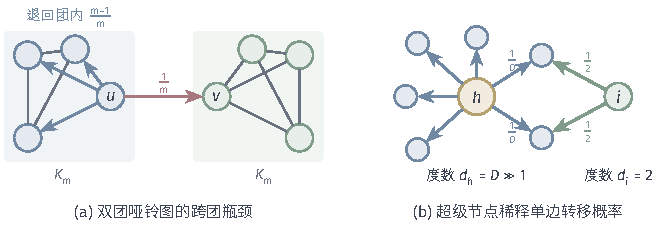
\includegraphics[width=111.633mm]{figures/03-graphs/05-matrices-and-spectra/tikz/laplacian-diffusion-bottleneck/figure.pdf}
  \caption{度数分布对一步随机游走转移概率的稀释效应。（a）双团哑铃图中，桥端点$u$有$m-1$条团内边和$1$条跨团桥边，粒子跨过桥边的概率仅为$1/m$，以$(m-1)/m$的概率退回原团。（b）度数为$D\gg 1$的枢纽顶点$h$将每条关联边上的转移概率稀释为$1/D$，而度数为$2$的普通节点$i$在每条边上分配$1/2$的转移概率。}
  \label{fig:laplacian-diffusion-bottleneck}
\end{BookInlineFigure}

在每步跳转一次的离散随机游走模型中，转移概率取决于边权占顶点加权度的比例，跨区瓶颈则与割权占集合体积$\operatorname{vol}(S)=\sum_{i\in S}d_i$的比例有关。归一化谱与这一时间尺度相适应。

为研究上述离散随机游走，使用度矩阵$\bm D$对拉普拉斯矩阵作归一化。本节先引入以度数计权的度加权内积与集合体积，再分别构造对称归一化拉普拉斯$\mathcal L=\bm D^{-1/2}\bm L\bm D^{-1/2}$和随机游走拉普拉斯$\bm L_{\mathrm{rw}}=\bm D^{-1}\bm L$，对比两种归一化算子的联系与分工，最后证明归一化拉普拉斯谱的性质。

\subsection{度加权内积}
\label{sec:graph-degree-weighted-inner-product}

标准欧氏长度平方$\sum_i x_i^2$给每个顶点相同的权重$1$。为了按每个顶点的连接量计权，将第$i$个坐标的权重替换为该顶点的加权度$d_i$，在正度顶点集$V_+=\{i\in V:d_i>0\}$上定义\term{度加权内积}（degree-weighted inner product）及其诱导范数：
\begin{equation}
  \langle \bm x,\bm y\rangle_{\bm D}
  =\bm x^\top\bm D\bm y
  =\sum_{i\in V_+}d_i\,x_iy_i,
  \qquad
  \lVert\bm x\rVert_{\bm D}^2=\bm x^\top\bm D\bm x.
  \label{eq:graph-degree-weighted-inner-product}
\end{equation}
在$V_+$上所有$d_i>0$，故任意非零向量的度加权长度平方$\lVert\bm x\rVert_{\bm D}^2>0$，式~\eqref{eq:graph-degree-weighted-inner-product}确实构成$V_+$上的内积。

用度加权范数衡量单点脉冲$\bm e_i$（$i\in V_+$）时，其沿边变化能量为$\bm e_i^\top\bm L\bm e_i=d_i$，度加权长度平方同样为$\lVert\bm e_i\rVert_{\bm D}^2=d_i$，两者之比对任意正度顶点都恒等于
\[
  \frac{\bm e_i^\top\bm L\bm e_i}{\lVert\bm e_i\rVert_{\bm D}^2}=\frac{d_i}{d_i}=1.
\]
例如在四点五边单位权图上，度为$3$的顶点$1$与度为$2$的顶点$2$在标准欧氏范数下的单位脉冲能量分别为$3$和$2$，而在度加权范数下，每单位连接量所承担的变化比值完全一致，均为$1$。

将任意顶点子集$S\subseteq V$的指示向量$\bm 1_S$代入度加权长度平方，立得子集内各顶点的加权度总和：
\begin{equation}
  \operatorname{vol}(S)=\sum_{i\in S}d_i
  =\lVert\bm1_S\rVert_{\bm D}^2.
  \label{eq:graph-laplacian-vertex-volume}
\end{equation}
这个和称为顶点子集$S$的\emph{体积}（volume），它精确计量了$S$所关联的边权容量：两端都在$S$内部的边在两个端点各计一次共两倍权重，跨出$S$的边计一倍权重。例如四点五边图中$S=\{1,2\}$的体积为$d_1+d_2=3+2=5$。

结合第~\ref{sec:graph-laplacian-energy}节的割权公式$\bm 1_S^\top\bm L\bm 1_S=c(S,V\setminus S)$，指示向量$\bm 1_S$的度加权Rayleigh商为
\[
  \frac{\bm 1_S^\top\bm L\bm 1_S}{\bm 1_S^\top\bm D\bm 1_S}
  =\frac{c(S,V\setminus S)}{\operatorname{vol}(S)}.
\]
这一比值直接给出了切开$S$的跨割边权重占$S$总连接体积的比例——这正是第~\ref{chap:spectral-partition}章导通率与归一化割（NCut）的核心度量。

需要注意，孤立顶点的加权度$d_i=0$，一个只在孤点上取$1$的非零向量在$\bm x^\top\bm D\bm x$下得零值，因此在包含孤点的全空间上$\sqrt{\bm x^\top\bm D\bm x}$只是半范数，相应双线性型不构成正定内积。下面的推导先在正度顶点集$V_+$上进行，再约定孤点在全空间矩阵中的零扩展。

\subsection{对称归一化拉普拉斯}
\label{sec:graph-symmetric-normalized-laplacian}

在$V_+$上，一组读数的能量与度加权长度平方之比为
\[
  \frac{\bm x^\top\bm L\bm x}{\bm x^\top\bm D\bm x},
  \qquad \bm x\ne\bm0.
\]
这是一个广义 Rayleigh 商。如果能把分母变成普通欧氏长度平方，就可以直接使用对称矩阵的谱分析工具。

观察分母中的每一项$d_ix_i^2$。它可以写成$(\sqrt{d_i}\,x_i)^2$。这就提示我们引入新坐标$y_i=\sqrt{d_i}\,x_i$。在正度顶点上，这个变换是可逆的：$x_i=y_i/\sqrt{d_i}$。新坐标描述的仍然是同一组读数，只是数值按度的平方根缩放了。

以四点图上的常值读数$x_i=1$为例。顶点$1$和$3$的度为$3$，对应新坐标为$\sqrt3$。顶点$2$和$4$的度为$2$，对应新坐标为$\sqrt2$。尽管四个新坐标的数值不同，还原后的实际读数仍然处处相等。

将$\bm x=\bm D^{-1/2}\bm y$代入分子，左右各出现一个$\bm D^{-1/2}$：
\[
  \bm x^\top\bm L\bm x
  =\bm y^\top(\bm D^{-1/2}\bm L\bm D^{-1/2})\bm y.
\]
分母已经变成$\bm y^\top\bm y$。整个比值成为新坐标上一个对称矩阵的普通 Rayleigh 商。矩阵极值性质可参考\BookChapterRef{chap:matrix-approximation}{卷二"矩阵逼近"章}。

\begin{definition}[对称归一化拉普拉斯]
\label{def:graph-symmetric-normalized-laplacian}
在正度顶点上，\term{对称归一化拉普拉斯}（symmetric normalized Laplacian）定义为
\begin{equation}
  \begin{aligned}
  \mathcal L&=\bm D^{-1/2}\bm L\bm D^{-1/2}\\
            &=\bm I-\bm D^{-1/2}\bm W\bm D^{-1/2}.
  \end{aligned}
  \label{eq:graph-symmetric-normalized-laplacian}
\end{equation}
含孤点时，在$\bm D^{-1/2}$中将孤点位置取零，用第一式定义全空间上的矩阵。
\end{definition}

在新坐标中，一条边比较的是$y_i/\sqrt{d_i}$和$y_j/\sqrt{d_j}$，即还原后的实际读数。因此，原读数在某个连通分量上取常值$1$、分量外取$0$时，新坐标中的零方向变为$\bm D^{1/2}\bm1_{V_a}$，即各点取$\sqrt{d_i}$。图~\ref{fig:laplacian-degree-coordinates}展示了四点图上常值读数的两种坐标。右图中四个坐标因度而异，但还原为实际读数后各边差值仍为零。

\begin{BookInlineFigure}
  \centering
  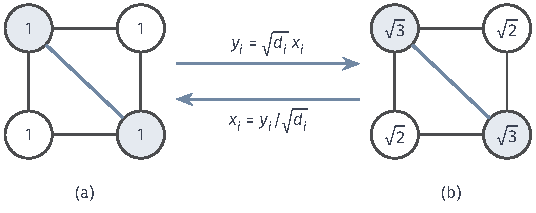
\includegraphics{figures/03-graphs/05-matrices-and-spectra/tikz/laplacian-degree-coordinates.pdf}
  \caption{同一组常值读数的两种坐标。浅蓝顶点度为三，白色顶点度为二。（a）原读数都为一。（b）按度的平方根缩放后，坐标因度而异。计算边差时，先按下方箭头把每个坐标还原。}
  \label{fig:laplacian-degree-coordinates}
\end{BookInlineFigure}

现在把孤点放回全空间。规定孤点在矩阵中有一行零、一列零，表示它的读数不参与任何邻居的计算。$\bm D^{-1/2}$在全空间中的对角矩阵于是在孤点位置取零。坐标的可逆换元仍然只在正度空间上使用。

如果按式~\eqref{eq:graph-symmetric-normalized-laplacian}的第二行来理解全空间矩阵，就需要注意单位阵的对应调整。在第一行中，$\bm D^{-1/2}\bm D\bm D^{-1/2}$在正度位置得到$1$，在孤点位置得到$0$。因此第二行的$\bm I$应当理解为$\bm\Pi_+$，即正度处取$1$、孤点处取$0$的对角投影阵。

用一个小例子核验。只在顶点$1,2$之间放一条单位权边，顶点$3$为孤点。$\bm D=\operatorname{diag}(1,1,0)$，按定义得到
\[
  \mathcal L=\begin{bmatrix}1&-1&0\\-1&1&0\\0&0&0\end{bmatrix}.
\]
零空间由$(1,1,0)^\top$和$(0,0,1)^\top$张成。如果错把孤点的对角元设成$1$，就会丢掉孤点对应的零方向。

\subsection{随机游走拉普拉斯}
\label{sec:graph-random-walk-laplacian}

归一化邻居平均提供了第二种视角。对正度顶点$i\in V_+$，将每个邻居的边权除以该点的总加权度$d_i$，所得$P_{i,j}=w_{i,j}/d_i$是邻居$j$在顶点$i$的所有连接中所占的权重份额。所有份额非负且总和为$\sum_j P_{i,j}=1$，因此
\begin{equation}
  (\bm P\bm x)_i=\sum_{j=1}^n\frac{w_{i,j}}{d_i}x_j
  \label{eq:graph-random-walk-neighbor-average}
\end{equation}
正是顶点$i$的邻居读数的加权平均。若某个顶点$i$是零度孤点（$d_i=0$），约定其保持原读数不变，即令$P_{i,i}=1$且$P_{i,j}=0$（$j\ne i$）。

\begin{definition}[随机游走拉普拉斯]
\label{def:graph-random-walk-laplacian}
设$\bm P$为按上述规则定义的邻域平均矩阵。图的\term{随机游走拉普拉斯}（random-walk Laplacian）定义为
\begin{equation}
  \bm L_{\mathrm{rw}}=\bm I-\bm P.
  \label{eq:graph-random-walk-laplacian}
\end{equation}
在正度顶点集$V_+$上，$\bm P=\bm D^{-1}\bm W$，从而$\bm L_{\mathrm{rw}}=\bm I-\bm D^{-1}\bm W=\bm D^{-1}\bm L$。
\end{definition}

随机游走拉普拉斯直接以原顶点读数$\bm x$为输入，在每个正度顶点$i$处输出本点读数$x_i$减去邻居加权平均$(\bm P\bm x)_i$的偏离量；在孤点处，因$(\bm P\bm x)_i=x_i$，输出恒为零。

在四点五边单位权图上取$\bm x=(1,0,1,0)^\top$核对：组合拉普拉斯输出为$\bm L\bm x=(2,-2,2,-2)^\top$，逐行除以各点度数$(3,2,3,2)$即得
\[
  \bm L_{\mathrm{rw}}\bm x=(2/3,-1,2/3,-1)^\top.
\]
逐点检查：顶点$1$的三个邻居$2,3,4$读数为$0,1,0$，平均值为$1/3$，本点读数$1$减去$1/3$得$2/3$；顶点$2$的两个邻居$1,3$读数均为$1$，平均值为$1$，本点读数$0$减去$1$得$-1$。

虽然在度数不均匀的图上，$\bm P=\bm D^{-1}\bm W$与$\bm L_{\mathrm{rw}}=\bm D^{-1}\bm L$在标准欧氏内积下一般不对称，但在正度空间$V_+$的度加权内积$\langle\cdot,\cdot\rangle_{\bm D}$下，它们都是自伴算子。事实上，由$\bm D\bm P=\bm W=\bm W^\top=\bm P^\top\bm D$，对任意$\bm x,\bm y\in\mathbb R^{V_+}$有
\[
  \begin{aligned}
    \langle \bm x,\bm P\bm y\rangle_{\bm D}
    &=\bm x^\top\bm D\bm P\bm y\\
    &=\bm x^\top\bm W\bm y\\
    &=(\bm P\bm x)^\top\bm D\bm y
     =\langle \bm P\bm x,\bm y\rangle_{\bm D}.
  \end{aligned}
\]

名称中的“随机游走”源于$P_{i,j}=w_{i,j}/d_i$的概率解释：将其视为从顶点$i$出发下一步随机移向邻居$j$的转移概率时，$(\bm P\bm x)_i$恰好是下一步所在顶点读数的条件期望。第~\ref{chap:graph-walks}章将围绕转移矩阵$\bm P$展开图上随机游走的分布演化与收敛分析。

\subsection{两种归一化拉普拉斯的对比}
\label{sec:graph-normalized-laplacian-comparison}

对称归一化拉普拉斯$\mathcal L=\bm D^{-1/2}\bm L\bm D^{-1/2}$与随机游走拉普拉斯$\bm L_{\mathrm{rw}}=\bm D^{-1}\bm L=\bm I-\bm P$从不同方式对度数作了归一化，二者在相似关系、对称性与应用场景上既有紧密联系，又有明确分工。

\paragraph{相似关系}
在正度空间$V_+$上，先用$\bm D^{-1/2}$把缩放坐标还原为原顶点读数，再作用$\bm L_{\mathrm{rw}}=\bm D^{-1}\bm L$，最后用$\bm D^{1/2}$转回缩放坐标，合并左侧的$\bm D^{1/2}\bm D^{-1}=\bm D^{-1/2}$即得相似恒等式
\begin{equation}
  \mathcal L=\bm D^{-1/2}\bm L\bm D^{-1/2}=\bm D^{1/2}\bm L_{\mathrm{rw}}\bm D^{-1/2}.
  \label{eq:graph-normalized-laplacian-similarity}
\end{equation}
因此，$\mathcal L$与$\bm L_{\mathrm{rw}}$在$V_+$上互为相似矩阵，拥有完全相同的特征值（连同每个零度孤点在两个矩阵中各自贡献的一个零特征值，两者在全空间上的谱也完全一致）。

两者的特征向量之间相差一个度平方根缩放因子：若$\bm x\in\mathbb R^{V_+}$满足$\bm L_{\mathrm{rw}}\bm x=\mu\bm x$，左乘$\bm D^{1/2}$即知$\bm y=\bm D^{1/2}\bm x$满足$\mathcal L\bm y=\mu\bm y$。特别地，对于零特征值$\mu=0$，$\bm L_{\mathrm{rw}}$在连通分量上的零特征向量是处处相等的常值向量$\bm 1_{V_a}$，而$\mathcal L$对应的零特征向量则是按度平方根加权的$\bm D^{1/2}\bm 1_{V_a}$。

\paragraph{对称性}
$\mathcal L$从左右两侧对称地乘上$\bm D^{-1/2}$，在标准欧氏内积$\langle\bm y,\bm y'\rangle=\bm y^\top\bm y'$下是实对称矩阵（$\mathcal L^\top=\mathcal L$），其不同特征子空间关于标准欧氏内积正交。

$\bm L_{\mathrm{rw}}=\bm D^{-1}\bm L$只在左侧乘以$\bm D^{-1}$，一般不对称；只有每条正权边的两端加权度相等时才对称（不同连通分量可以有不同的度）；但它在度加权内积$\langle\bm x,\bm x'\rangle_{\bm D}=\bm x^\top\bm D\bm x'$下自伴，可选取关于度加权内积$\bm D$-正交的特征向量基，这恰好对应缩放后的向量$\bm y=\bm D^{1/2}\bm x$关于标准欧氏内积正交。

\paragraph{应用场景}
当需要利用实对称矩阵的正交谱分解、Courant--Fischer极小极大原理或矩阵范数工具（例如第~\ref{chap:spectral-partition}章求解归一化割NCut的谱松弛与第~\ref{chap:graph-sparsification}章的谱稀疏化）时，采用实对称的$\mathcal L$最为直接。

当需要直接对原顶点函数作局部邻域加权平均、或追踪概率分布在图上一步步扩散的马尔可夫链演化（例如第~\ref{chap:graph-walks}章的随机游走与PageRank）时，采用保持行和为零的$\bm L_{\mathrm{rw}}=\bm I-\bm P$更为自然。当图为正度$d$正则图时，$\bm D=d\bm I$，两种归一化矩阵合二为一，均简化为$\mathcal L=\bm L_{\mathrm{rw}}=\bm L/d$。

\subsection{归一化拉普拉斯谱的性质}
\label{sec:graph-normalized-laplacian-spectrum}

由于$\mathcal L$与$\bm L_{\mathrm{rw}}$具有相同的特征值，我们统称其为图的\emph{归一化拉普拉斯谱}。下面的定理证明，按度归一化后，任意图的全部特征值都被收束在无量纲的固定区间$[0,2]$内，且上界$\mu=2$直接刻画了图的二部性。

\begin{theorem}[归一化拉普拉斯谱的范围]
\label{prop:graph-normalized-spectrum-bound}
有限无向非负加权图的对称归一化拉普拉斯$\mathcal L$（以及随机游走拉普拉斯$\bm L_{\mathrm{rw}}$）的全部特征值$\mu$均满足
\begin{equation}
  0\leq\mu\leq2.
  \label{eq:graph-normalized-spectrum-bound}
\end{equation}
其中零特征值的重数等于正权支撑$\mathcal G_+$的连通分量个数$c$；最大特征值达到上界$\mu=2$当且仅当正权支撑$\mathcal G_+$至少含有一个带正权边的二部连通分量。
\end{theorem}

\begin{proof}
第一步，将特征值写为度加权Rayleigh商并确定下界与零特征值重数。孤立顶点在$\mathcal L$和$\bm L_{\mathrm{rw}}$上均对应零特征值且自成无边的连通分量，故只需在正度顶点集$V_+$上分析。设非零向量$\bm x\in\mathbb R^{V_+}$满足$\bm L_{\mathrm{rw}}\bm x=\mu\bm x$，即$\bm D^{-1}\bm L\bm x=\mu\bm x$。左乘$\bm x^\top\bm D$并除以$\bm x^\top\bm D\bm x>0$，得
\[
  \mu=\frac{\bm x^\top\bm L\bm x}{\bm x^\top\bm D\bm x}
  =\frac{\sum_{\{i,j\}\in E}w_{i,j}(x_i-x_j)^2}{\sum_{i\in V_+}d_i x_i^2}.
\]
分子非负给出$\mu\geq 0$；且$\mu=0\iff\bm x^\top\bm L\bm x=0$，由定理~\ref{thm:graph-laplacian-components}知这等价于$\bm x$在每个正权连通分量上取常值，连同孤点在内零特征值重数恰为$c$。

第二步，证明上界$\mu\leq 2$。将$2\bm x^\top\bm D\bm x=2\sum_{i\in V_+}d_i x_i^2=\sum_{\{i,j\}\in E}2w_{i,j}(x_i^2+x_j^2)$与分子$\bm x^\top\bm L\bm x=\sum_{\{i,j\}\in E}w_{i,j}(x_i-x_j)^2$作差，利用代数恒等式$2(x_i^2+x_j^2)-(x_i-x_j)^2=(x_i+x_j)^2$，得到
\[
  2\bm x^\top\bm D\bm x-\bm x^\top\bm L\bm x
  =\sum_{\{i,j\}\in E}w_{i,j}(x_i+x_j)^2\geq 0.
\]
两端除以$\bm x^\top\bm D\bm x>0$即得$2-\mu\geq 0$，即$\mu\leq 2$。

第三步，分析取等号$\mu=2$的充要条件。上式取等号当且仅当存在非零向量$\bm x\in\mathbb R^{V_+}$使得$\sum_{\{i,j\}\in E}w_{i,j}(x_i+x_j)^2=0$，即对每条正权边$\{i,j\}\in E_+$都有$x_i+x_j=0$（$x_j=-x_i$）。

若$\mu=2$，任取$\bm x$的一个非零分量顶点$u\in V_+$，其所在正权连通分量$C$至少含有一条正权边。沿$C$中的任意正权路径每走一步，顶点读数变为相反数，故$C$中所有顶点的读数均取$\pm|x_u|\neq 0$，且每条正权边都连接一个取$+|x_u|$的顶点和一个取$-|x_u|$的顶点；将$C$按读数的正负号划分为两部分，即知$C$为含边的二部连通分量。

反之，若$\mathcal G_+$含有一个带边的二部连通分量$C=A\cup B$，令$\bm x$在$A$上取$+1$、在$B$上取$-1$、在其余分量上取$0$，则$\bm x\in\mathbb R^{V_+}$非零且在每条正权边上满足$x_i+x_j=0$，其度加权Rayleigh商达到$\mu=2$。
\end{proof}

这一结论可与第~\ref{sec:adjacency-bipartite-symmetry}小节二部图邻接谱的对称性对照：在四点单位权图上，四元环$C_4$是二部图，沿环交替赋$+1,-1$即可使每条边两端互为相反数，达到$\mu=2$；添入对角边$13$后，顶点$1$和$3$被连入同一个三角形，无法再为三个两两相邻的顶点同时赋予互为相反数的非零值，故四点五边图的归一化拉普拉斯最大特征值严格小于$2$。

最后考察边权整体缩放：若将全图所有边权同时乘以正数$a>0$，则$\bm L$和$\bm D$同时乘以$a$，$\mathcal L=\bm D^{-1/2}\bm L\bm D^{-1/2}$中两侧的$a^{-1/2}$与中间的$a$恰好抵消，随机游走矩阵$\bm P=\bm D^{-1}\bm W$也保持不变，说明归一化谱完全消除了边权的整体量纲尺度。例如四元环$C_4$的组合拉普拉斯谱为$0,2,2,4$，除以正则度数$d=2$即得归一化谱$0,1,1,2$，无论把四条边的权重同时改为何种正数，这一归一化谱始终不变。

\section{本章小结}
\label{sec:graph-laplacian-summary}

组合拉普拉斯把沿边取差、乘权和返回顶点三个步骤合成为$\bm L=\bm B\bm C\bm B^\top$。逐点来看，它输出的是每个顶点与邻居的带权偏离之和。若要衡量整张图上读数的变化而不让正负相消，就逐边取差、平方、乘权再求和。这个沿边变化能量恰好等于拉普拉斯的二次型$\bm x^\top\bm L\bm x$。

能量为零要求每条正权边的两端读数相等。沿正权路径传递这个等值关系，每个连通分量上的读数各为常值，分量之间可以独立选择。分量的个数就是零特征值的重数。

按边集展开约化拉普拉斯的行列式时，只有构成生成树的边组留下非零的关联子式。因此，删去任一个顶点对应的行和列后所得的主余子式都给出同一个树权总和。对正权支撑连通的图，也可以用$n-1$个非零特征值的乘积除以顶点数$n$来计算它。

每个特征值还描述了对应单位特征向量的变化尺度——长度为一的读数方向上的沿边能量。加边使每个方向的单位能量不减，进而使按大小排序的各特征值逐个不减。

三种矩阵使用不同的内积和坐标。组合拉普拉斯$\bm L=\bm D-\bm W$在原顶点读数上计算带权差的总和。随机游走拉普拉斯$\bm L_{\mathrm{rw}}=\bm I-\bm P$用同样的原顶点读数，输出的是本点读数与邻居加权平均的差。对称归一化拉普拉斯$\mathcal L=\bm D^{-1/2}\bm L\bm D^{-1/2}$在缩放坐标$\bm y=\bm D^{1/2}\bm x$上计算，使得度加权能量比变成普通 Rayleigh 商。三种形式的零方向都来自各分量上的常值读数——在原坐标中是分量指示向量$\bm1_{V_a}$，在缩放坐标中变为$\bm D^{1/2}\bm1_{V_a}$。三种矩阵都对孤点留出零块。

后续各章使用的矩阵形式各不相同。第~\ref{chap:graph-electrical-networks}章的电网络从注入电流出发求电势，方程的系数是组合拉普拉斯。第~\ref{chap:spectral-partition}章要比较连接量不同的顶点集合两侧的割与体积，归一化形式提供了按体积计量的尺度。第~\ref{chap:graph-walks}章用转移矩阵$\bm P$描述逐步选择邻居的演化，从邻居平均出发的收敛分析建立在归一化谱之上。


\chapter{电网络}
\label{chap:graph-electrical-networks}

在四点环加对角边$13$的图上，从顶点$1$送入一单位电流，从顶点$3$取出。电流可以直接走对角边，也可以沿环上的两条外侧支路绕行。怎样在这些支路之间分配电流，取决于各条边的电阻。分配确定后，维持单位电流所需要的两端电势差，就概括了整张网络对这一对顶点的作用。

我们先分别写出逐边的电势与电流关系，以及逐点的流入流出平衡。把两个条件联立后，未知量只剩各顶点的电势，系数矩阵正是第~\ref{chap:graph-laplacian-matrix}章的组合拉普拉斯。解出电势，就能沿边恢复电流。

还可以把不同的分流方案放在一起比较耗散。在给定注入下，实际电流是所有守恒分流中耗散最小的，这就是Thomson原理。从单位分流所需的端点压降，可以引出有效电阻。它在后面的稀疏化抽样与往返时间计算中都有直接用途。

\section{电网络的基本定律}
\label{sec:electrical-network-laws}

把带正权边的无向图看成\term{电网络}（electrical network）：每条正权边是一个电阻元件，顶点是这些元件连接的接点，外部可以在指定接点注入或取出电流。我们先从一个接点看各条边的净流量，建立电流守恒方程；再从一条边看两端电势怎样决定流过它的电流，写出Ohm定律。

\subsection{电流守恒}
\label{sec:electrical-current-conservation}

一条边导电的容易程度用\term{电导}（conductance）$c_e = w_e > 0$来衡量，倒数$r_e = 1/c_e$是\term{电阻}（resistance）。电导越大，同样的电势差下流过的电流越多。零权边不导电，删去它们后保留的图称为正权支撑。正权支撑仍包括所有顶点，即使某个顶点不再与任何正权边相邻。

设顶点数为$n$，正权边数为$m$。每条边记录一个带符号的电流，组成向量$\bm f\in\mathbb R^m$。记录方向沿用第~\ref{chap:graph-incidence-matrix}章的约定：关联矩阵$\bm B\in\mathbb R^{n\times m}$的每列在尾端取$+1$、头端取$-1$。$f_e > 0$表示电流沿记录方向流动，$f_e < 0$表示实际流向与记录相反。

以四点图为例。边$41$的记录方向为$4\to1$。若边上流量为$-2$，实际含义是$2$个单位的电流从$1$流向$4$。看顶点$1$，这条边从外面带来了$2$个单位的电流。

每个顶点的进出必须平衡。由关联矩阵按行读取，顶点$i$在出发边上取$+f_e$，在到达边上取$-f_e$，各项相加得到净流出量$(\bm B\bm f)_i$。假设两条边的记录方向都朝外，其流量分别为$3$和$-1$。实际上前者送出$3$，后者从外面送入$1$，净流出$3 - 1 = 2$。

外部在顶点$i$注入电流$b_i$，这些电流必须从该点流向网络内部。$b_i > 0$是注入，$b_i < 0$是引出。\term{Kirchhoff电流定律}（Kirchhoff's current law）要求每个顶点的网络净流出等于外部注入：
\begin{equation}
  \bm B\bm f = \bm b.
  \label{eq:electrical-current-conservation}
\end{equation}
上面那个接点的净流出为$2$，所以外部恰好需要送入$b_i = 2$单位电流来维持平衡。

图~\ref{fig:electrical-local-current-balance}把同一个接点的电流守恒用两种方式画出来。左图用记录方向和带符号的数值。右图把方向转成实际流向，在接点处画出外部注入的量。

\begin{BookInlineFigure}
  \centering
  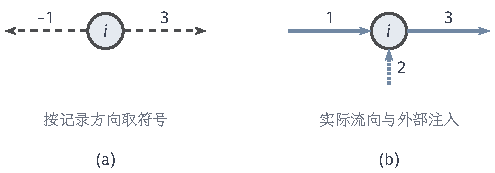
\includegraphics[scale=1]{figures/03-graphs/05-matrices-and-spectra/tikz/electrical-local-current-balance/figure.pdf}
  \caption{接点的电流守恒。(a)~虚线箭头给出两条边的记录方向，左边的负号表示逆向流动。(b)~两条实线箭头给出真实流向，下方点线箭头给出维持守恒所需的外部注入量。}
  \label{fig:electrical-local-current-balance}
\end{BookInlineFigure}

把式~\eqref{eq:electrical-current-conservation}的$n$个方程按顶点求和。每条边在尾端贡献$+f_e$，在头端贡献$-f_e$，两者抵消。因此全图的外部注入总和必须为零：
\[
  \sum_{i=1}^n b_i = \bm 1^\top \bm b = 0.
\]
对单个连通分量也一样——如果两个分量之间没有正电导边，电流就无法从一个分量穿越到另一个。每个正权连通分量必须各自满足注入总量为零。

\subsection{Ohm定律}
\label{sec:electrical-ohm-law}

守恒只限制流入和流出的总量，还没有决定每条边上有多少电流。每条边的电流由两端的电势差和该边的电导共同决定。

给每个顶点一个电势值$v_i$，组成向量$\bm v\in\mathbb R^n$。沿边$e\colon i\to j$看，电势从$v_i$变到$v_j$，沿记录方向的压降为$v_i - v_j$。例如$v_i = 3$、$v_j = 1$，压降为$2$。若这条边的电导为$c_e = 1/2$，\term{Ohm定律}（Ohm's law）给出流过它的电流：
\[
  f_e = c_e(v_i - v_j) = \tfrac{1}{2} \times 2 = 1.
\]
压降越大或电导越大，电流越大。

对所有记录边一起取差，得到压降向量$\bm B^\top\bm v$。再在每条边上乘以该边的电导，便得到全部电流：
\begin{equation}
  \bm f = \bm C\bm B^\top\bm v, \qquad \bm C = \operatorname{diag}(c_e\colon e\in E).
  \label{eq:electrical-ohm-law}
\end{equation}

沿任一闭环累计压降，中间顶点的电势在前一步的末端和后一步的始端各出现一次，正好抵消。在四点图上，沿$1\to2\to3\to1$走一圈：
\[
  (v_1 - v_2) + (v_2 - v_3) + (v_3 - v_1) = 0.
\]
这就是\term{Kirchhoff电压定律}（Kirchhoff's voltage law）。它说明由顶点电势产生的压降向量一定落在第~\ref{chap:graph-incidence-matrix}章的割空间$\operatorname{im}\bm B^\top$中。沿环检验时，若已知边电流$f_e$，先乘电阻得到压降$r_e f_e$，再按行进方向加减。

把所有电势同时加上同一个常数$c$，各条边的压降为$(v_i + c) - (v_j + c) = v_i - v_j$，保持不变。因此电流也不会改变。这个常数自由度说明，单靠注入量无法唯一确定电势本身，但可以确定电势差和边电流。下一节求解时，我们会选一个顶点固定电势基准来消去这个自由度。

\section{拉普拉斯方程的求解}
\label{sec:graph-laplacian-solve}

给定各顶点的外部注入电流$\bm b\in\mathbb R^n$，将上一节的Ohm定律与Kirchhoff电流定律联立，即可导出仅含顶点电势$\bm v\in\mathbb R^n$的线性方程组。具体分三步完成：

第一步，用顶点电势表示边压降。由关联矩阵转置的作用，全图$m$条有向参考边上的压降向量为$\Delta\bm v = \bm B^\top\bm v$，其中第$e\colon i\to j$条边的分量为$v_i - v_j$。

第二步，由Ohm定律写出边电流。将每条边的压降乘以该边电导$c_e$，得到边电流向量式~\eqref{eq:electrical-ohm-law}：
\[
  \bm f = \bm C\bm B^\top\bm v.
\]

第三步，代入Kirchhoff电流定律。将$\bm f = \bm C\bm B^\top\bm v$代入守恒方程$\bm B\bm f = \bm b$，消去中间变量$\bm f$，得到
\[
  \bm B\bm C\bm B^\top\bm v = \bm b.
\]
对比第~\ref{sec:graph-laplacian}节的关联矩阵分解式~\eqref{eq:graph-laplacian-incidence-factorization}，左侧的复合矩阵$\bm B\bm C\bm B^\top$正是图的组合拉普拉斯矩阵$\bm L=\bm D-\bm W$（其中边权取为电导$w_{i,j}=c_{i,j}$）。于是电网络的平衡条件归结为如下\emph{拉普拉斯方程}：
\begin{equation}
  \bm L\bm v = \bm b, \qquad \bm L = \bm B\bm C\bm B^\top = \bm D - \bm W.
  \label{eq:electrical-laplacian-system}
\end{equation}
按第$i$个顶点展开，式~\eqref{eq:electrical-laplacian-system}的第$i$行方程为
\[
  (\bm L\bm v)_i = \sum_{j=1}^n c_{i,j}(v_i - v_j) = d_i v_i - \sum_{j=1}^n c_{i,j}v_j = b_i,
\]
其物理含义十分直观：从顶点$i$经所有相邻电阻支路流向邻居的电流之和$\sum_j c_{i,j}(v_i-v_j)$，必须等于外部在顶点$i$注入的电流$b_i$。

本节先证明拉普拉斯方程$\bm L\bm v=\bm b$的可解性充要条件与解空间结构，再说明如何通过选定一个接地点消去电势的常数平移自由度以获得唯一解，随后介绍一般网络的数值求解方法，最后给出树网络上的线性时间求解算法。

\subsection{拉普拉斯方程的可解性}
\label{sec:electrical-laplacian-derivation}

因为组合拉普拉斯矩阵$\bm L$满足$\bm L\bm 1=\bm 0$，它是奇异矩阵（不可逆），并非对任意右端向量$\bm b$都有解。下面的定理给出了拉普拉斯方程$\bm L\bm v=\bm b$有解的充要条件以及全部解的结构。

\begin{theorem}[拉普拉斯方程的可解性与解集结构]
\label{thm:electrical-laplacian-solvability}
设有限无向电网络的正权支撑连通，组合拉普拉斯矩阵为$\bm L\in\mathbb R^{n\times n}$。
\begin{enumerate}
  \item 线性方程组$\bm L\bm v=\bm b$有解，当且仅当全图外部注入电流的总和为零：
  \begin{equation}
    \bm 1^\top\bm b = \sum_{i=1}^n b_i = 0.
    \label{eq:electrical-zero-sum-condition}
  \end{equation}
  \item 当$\bm 1^\top\bm b=0$时，若$\bm v_0$是一个特解，则方程组$\bm L\bm v=\bm b$的通解为
  \[
    \bm v = \bm v_0 + c\bm 1 \qquad (c\in\mathbb R),
  \]
  即任意两组电势解仅相差一个全局常数平移$c\bm 1$；所有电势解经Ohm定律生成的边电流向量$\bm f=\bm C\bm B^\top\bm v$唯一确定。
  \item 在满足$\bm 1^\top\bm v=0$的零均值子空间$\bm 1^\perp$内，方程组$\bm L\bm v=\bm b$存在唯一解，由Moore--Penrose伪逆给出：$\bm v_{\mathrm{zm}} = \bm L^\dagger\bm b$。
\end{enumerate}
\end{theorem}

\begin{proof}
（1）由定理~\ref{thm:graph-laplacian-components}，当正权支撑连通时，$\bm L$的零空间为一维常向量空间$\ker\bm L=\operatorname{span}\{\bm 1\}$。由于$\bm L$是实对称矩阵，其列空间（像空间）等于零空间的正交补：
\[
  \operatorname{im}\bm L = (\ker\bm L)^\perp = \bm 1^\perp = \Bigl\{\bm b\in\mathbb R^n : \bm 1^\top\bm b = 0\Bigr\}.
\]
因此$\bm b\in\operatorname{im}\bm L$（即$\bm L\bm v=\bm b$有解）当且仅当$\bm 1^\top\bm b = 0$。

（2）设$\bm v_1,\bm v_2$均满足$\bm L\bm v=\bm b$，作差得$\bm L(\bm v_1-\bm v_2)=\bm 0$，即$\bm v_1-\bm v_2\in\ker\bm L=\operatorname{span}\{\bm 1\}$，故存在常数$c\in\mathbb R$使得$\bm v_2=\bm v_1+c\bm 1$。代入Ohm定律，因$\bm B^\top\bm 1=\bm 0$，有
\[
  \bm C\bm B^\top\bm v_2 = \bm C\bm B^\top(\bm v_1 + c\bm 1) = \bm C\bm B^\top\bm v_1,
\]
故边电流向量唯一确定。

（3）由于$\ker\bm L=\operatorname{span}\{\bm 1\}$且$\operatorname{im}\bm L=\bm 1^\perp$，$\bm L$限制在不变子空间$\bm 1^\perp$上是到自身的对称正定可逆算子（$n\geq2$时最小特征值为$\lambda_2>0$；单点网络的零和空间只有零向量），其逆算子在$\bm 1^\perp$上正是Moore--Penrose伪逆$\bm L^\dagger$，故唯一零均值解为$\bm v_{\mathrm{zm}}=\bm L^\dagger\bm b$。
\end{proof}

若正权支撑不连通，有$c$个连通分量$V_1,\ldots,V_c$，则由$\ker\bm L=\operatorname{span}\{\bm 1_{V_1},\ldots,\bm 1_{V_c}\}$可知：$\bm L\bm v=\bm b$有解当且仅当每个连通分量内部的外部注入总和各自为零（$\bm 1_{V_a}^\top\bm b=0$，$a=1,\ldots,c$），此时各连通分量的电势可独立平移各自的常数。

\subsection{接地与唯一解}
\label{sec:electrical-grounding}

定理~\ref{thm:electrical-laplacian-solvability}表明，在连通网络中，同一组相容注入$\bm b$对应无穷多组相差常数平移的电势解。为了在实际计算中直接通过可逆方阵唯一解出各点电势，最简便的做法是选定某个参考顶点$q\in V$，将其电势固定为零：
\[
  v_q = 0.
\]
这一操作称为在顶点$q$处\term{接地}（grounding）。例如三点电势$(5,3,2)^\top$在第三个顶点接地后，整体减去基准值$2$，即唯一确定为$(3,1,0)^\top$。

在选定接地点$q$并令$v_q=0$后，第$q$列在矩阵乘积$\bm L\bm v$中的贡献恒为$v_q\bm L_{:,q}=\bm 0$，因此可以直接删去$\bm L$的第$q$列；同时，由于全部$n$个顶点的守恒方程之和恒为零，只要其余$n-1$个顶点的守恒方程得到满足，第$q$个顶点的守恒方程就会自动满足，因此也可以删去$\bm L$的第$q$行。记从$\bm L$中删去第$q$行和第$q$列所得的$(n-1)\times(n-1)$主子矩阵为$\overline{\bm L}$，同时从$\bm v$和$\bm b$中删去第$q$个分量得到$\overline{\bm v},\overline{\bm b}\in\mathbb R^{n-1}$。

需要特别注意，删去第$q$行和第$q$列并不意味着把接地点$q$关联的边从电路中剪断：若边$e$连接保留顶点$i$与接地点$q$，它在第$i$行方程中原本贡献$c_e(v_i - v_q)$，代入$v_q = 0$后变为$c_e v_i$，该电导$c_e$依然保留在$\overline{\bm L}$的第$i$个对角元$d_i$中。

\begin{theorem}[接地约化系统的正定性与唯一解]
\label{prop:electrical-grounded-system}
设有限无向电网络的正权支撑连通，任选顶点$q\in V$接地（令$v_q=0$）。则删去$\bm L$的第$q$行和第$q$列所得的约化拉普拉斯矩阵$\overline{\bm L}\in\mathbb R^{(n-1)\times(n-1)}$是对称正定矩阵。对任意满足$\bm 1^\top\bm b=0$的注入向量$\bm b\in\mathbb R^n$，约化方程组
\begin{equation}
  \overline{\bm L}\,\overline{\bm v} = \overline{\bm b}
  \label{eq:electrical-grounded-system}
\end{equation}
存在唯一解$\overline{\bm v}=\overline{\bm L}^{-1}\overline{\bm b}$；将其在第$q$个位置补入$v_q=0$后，即得原方程组$\bm L\bm v=\bm b$满足$v_q=0$的唯一电势解。
\end{theorem}

\begin{proof}
第一步，证明$\overline{\bm L}$对称正定。$\overline{\bm L}$作为实对称矩阵$\bm L$的主子矩阵显然对称。任取非零向量$\overline{\bm x}\in\mathbb R^{n-1}$，在第$q$个位置补入$x_q=0$延拓为$n$维向量$\bm x\in\mathbb R^n$。由于$\overline{\bm x}\neq\bm 0$而$x_q=0$，$\bm x$的各个分量不全相等，故$\bm x\notin\operatorname{span}\{\bm 1\}=\ker\bm L$。由定理~\ref{prop:graph-laplacian-quadratic-form}(1)与定理~\ref{thm:graph-laplacian-components}，得
\[
  \overline{\bm x}^\top \overline{\bm L}\,\overline{\bm x}
  = \bm x^\top \bm L \bm x > 0.
\]
因此$\overline{\bm L}$是对称正定矩阵，从而可逆（这也与第~\ref{sec:graph-matrix-tree-proof}小节矩阵树定理给出的$\det\overline{\bm L}>0$一致）。

第二步，验证补入$v_q=0$后的向量$\bm v$满足全部$n$行方程$\bm L\bm v=\bm b$。令$\overline{\bm v}=\overline{\bm L}^{-1}\overline{\bm b}$并在第$q$个分量补入$v_q=0$得到$\bm v\in\mathbb R^n$。因为$v_q=0$，乘积$\bm L\bm v$中第$q$列不产生贡献，故在除$q$以外的$n-1$行上已有$(\bm L\bm v)_i=(\overline{\bm L}\,\overline{\bm v})_i=b_i$（$i\neq q$）。

对于被删去的第$q$行，利用$\bm 1^\top\bm L=\bm 0^\top$与相容条件$\bm 1^\top\bm b=0$，全体$n$个分量的残差之和满足
\[
  \sum_{i=1}^n\bigl((\bm L\bm v)_i - b_i\bigr)
  = \bm 1^\top(\bm L\bm v - \bm b)
  = (\bm 1^\top\bm L)\bm v - \bm 1^\top\bm b = 0.
\]
既然其余$n-1$项残差$(\bm L\bm v)_i-b_i$（$i\neq q$）全为零，第$q$项残差$(\bm L\bm v)_q-b_q$也必然为零，故$\bm L\bm v=\bm b$成立。由定理~\ref{thm:electrical-laplacian-solvability}(2)，满足$v_q=0$的解显然唯一。
\end{proof}

若已求出接地解$\bm v$，只需将每个分量减去全体分量的算术平均值$\bar v = \frac1n\bm 1^\top\bm v$，即可立刻得到定理~\ref{thm:electrical-laplacian-solvability}(3)中的零均值解$\bm v_{\mathrm{zm}}=\bm L^\dagger\bm b = \bm v - \bar v\bm 1$。

\begin{example}[四点电网络的接地求解]
\label{ex:electrical-four-vertex-network}
在四点环加对角边$13$的网络中，五条边均取单位电导$c_e=1$，边的参考方向依次为$1\to2$、$2\to3$、$3\to4$、$4\to1$、$1\to3$。在顶点$1$注入$1$单位电流，从顶点$3$引出$1$单位电流，顶点$2,4$无外部注入，即$\bm b=(1,0,-1,0)^\top$（满足$\bm 1^\top\bm b=0$）。选顶点$3$接地，令$v_3 = 0$。

第一步，写出接地后的$3\times 3$约化系统（图~\ref{fig:electrical-grounded-matrix}）。删去$\bm L$的第$3$行和第$3$列，保留顶点$1,2,4$的未知量$\overline{\bm v}=(v_1,v_2,v_4)^\top$与右端$\overline{\bm b}=(1,0,0)^\top$，得到
\[
  \begin{bmatrix}
    3 & -1 & -1\\
    -1 & 2 & 0\\
    -1 & 0 & 2
  \end{bmatrix}
  \begin{bmatrix}
    v_1\\ v_2\\ v_4
  \end{bmatrix}
  =
  \begin{bmatrix}
    1\\ 0\\ 0
  \end{bmatrix}.
\]

第二步，逐行消元求解电势。由第二行$-v_1+2v_2=0$和第三行$-v_1+2v_4=0$，得
\[
  v_2 = \frac{v_1}{2},\qquad v_4 = \frac{v_1}{2}.
\]
代入第一行$3v_1 - v_2 - v_4 = 1$，得$3v_1 - \frac12 v_1 - \frac12 v_1 = 2v_1 = 1$，解得$v_1 = 1/2$，从而$v_2 = v_4 = 1/4$。补回接地点$v_3=0$，得完整电势向量
\[
  \bm v = (1/2, \; 1/4, \; 0, \; 1/4)^\top.
\]

第三步，由Ohm定律恢复各边电流。沿五条有向参考边依次计算$f_e = c_e(v_i - v_j)$：
\[
  \begin{aligned}
    f_{12} &= v_1 - v_2 = \tfrac12 - \tfrac14 = \tfrac14,\qquad
    f_{23} = v_2 - v_3 = \tfrac14 - 0 = \tfrac14,\\
    f_{34} &= v_3 - v_4 = 0 - \tfrac14 = -\tfrac14,\qquad
    f_{41} = v_4 - v_1 = \tfrac14 - \tfrac12 = -\tfrac14,\\
    f_{13} &= v_1 - v_3 = \tfrac12 - 0 = \tfrac12.
  \end{aligned}
\]
其中$f_{34}=-1/4$和$f_{41}=-1/4$的负号表示实际电流为$1/4$，方向分别为$4\to 3$和$1\to 4$。排成边电流向量即为
\[
  \bm f = (1/4, \; 1/4, \; -1/4, \; -1/4, \; 1/2)^\top.
\]
逐点核对净流出：顶点$1$向两条外侧支路各送出$1/4$、向对角边送出$1/2$，总流出为$1$；顶点$2$和$4$各自从$1$接收$1/4$后转交给$3$，净流出为$0$；顶点$3$从三条支路合收$1/4+1/4+1/2=1$（净流出为$-1$），与$\bm b$完全一致。
\end{example}

图~\ref{fig:electrical-grounded-matrix}展示了例~\ref{ex:electrical-four-vertex-network}接地前后的矩阵方程：上方全系统中蓝色列对应已固定为$v_3=0$的列，黄色行对应冗余的第$3$行守恒方程；删去第$3$行和第$3$列后即得下方的$3\times 3$正定约化系统。图~\ref{fig:electrical-grounding-overview}与图~\ref{fig:electrical-current-split}展示了求解所得的电势分布与支路分流。

\begin{BookInlineFigure}
  \centering
  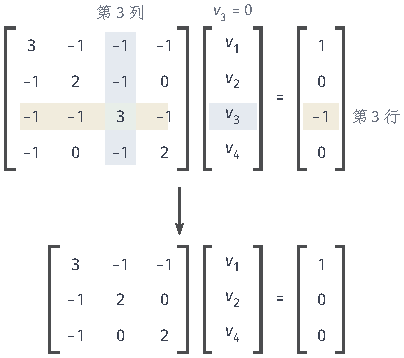
\includegraphics[scale=1]{figures/03-graphs/05-matrices-and-spectra/tikz/electrical-grounded-matrix/figure.pdf}
  \caption{在顶点$3$接地。上方是四点网络的全系统，蓝色竖带标出乘$v_3$的一列，黄色横带标出顶点$3$的方程。约化系统保留顶点$1,2,4$的未知量和守恒式。}
  \label{fig:electrical-grounded-matrix}
\end{BookInlineFigure}

\begin{figure}[!htb]
\centering
\begin{tikzpicture}[x=1mm,y=1mm,>=Stealth,
  vertex/.style={circle,draw=FigureBlue,fill=FigureBlueFill,inner sep=0pt,
    minimum size=5.5mm,line width=.52pt,font=\figurefont\fontsize{8}{10}\selectfont},
  gnd/.style={vertex,fill=FigureBlueFill,draw=FigureBlue,line width=.72pt},
  inject/.style={vertex,fill=FigureYellowFill,draw=FigureYellow,line width=.72pt},
  elabel/.style={font=\figurefont\fontsize{7}{8.5}\selectfont,FigureInk},
  vlabel/.style={font=\figurefont\fontsize{7.5}{9}\selectfont,FigureInk},
  panel/.style={anchor=mid,font=\figurefont\footnotesize}]
  % Left: setup
  \begin{scope}[xshift=0mm]
    \node[inject] (l1) at (0,14) {$1$};
    \node[vertex] (l2) at (14,14) {$2$};
    \node[gnd]    (l3) at (14,0) {$3$};
    \node[vertex] (l4) at (0,0) {$4$};
    \draw[FigureStroke,line width=.45pt] (l1)--(l2) (l2)--(l3) (l3)--(l4) (l4)--(l1) (l1)--(l3);
    \draw[->,FigureYellow,line width=.8pt] (-6,14) -- (l1) node[vlabel,midway,above] {$+1$};
    \draw[->,FigureBlue,line width=.8pt]  (l3) -- (20,0) node[vlabel,midway,above] {$-1$};
    \node[vlabel,below=1mm] at (l3.south) {接地};
    \node[panel] at (7,-8) {(a) 注入与接地};
  \end{scope}
  % Arrow
  \draw[->,FigureStroke,line width=.7pt] (26,7) -- (38,7) node[midway,above,font=\figurefont\fontsize{7}{8.5}\selectfont] {求解};
  % Right: solution
  \begin{scope}[xshift=44mm]
    \node[inject] (r1) at (0,14) {$1$};
    \node[vertex] (r2) at (14,14) {$2$};
    \node[gnd]    (r3) at (14,0) {$3$};
    \node[vertex] (r4) at (0,0) {$4$};
    \draw[FigureStroke,line width=.45pt] (r1)--(r2) (r2)--(r3) (r3)--(r4) (r4)--(r1) (r1)--(r3);
    \node[vlabel,left=1.5mm] at (r1) {$\frac{1}{2}$};
    \node[vlabel,right=1.5mm] at (r2) {$\frac{1}{4}$};
    \node[vlabel,right=1.5mm] at (r3) {$0$};
    \node[vlabel,left=1.5mm] at (r4) {$\frac{1}{4}$};
    % Current arrows
    \draw[->,FigureBlue,line width=.65pt] ([xshift=.5mm,yshift=-1mm]r1.east) -- ([xshift=-.5mm,yshift=-1mm]r2.west) node[elabel,above=.5mm,midway] {$\frac{1}{4}$};
    \draw[->,FigureBlue,line width=.65pt] ([xshift=-1mm,yshift=.5mm]r2.south) -- ([xshift=-1mm,yshift=-.5mm]r3.north) node[elabel,left=.5mm,midway] {$\frac{1}{4}$};
    \draw[->,FigureBlue,line width=.65pt] ([xshift=1mm,yshift=.5mm]r4.north) -- ([xshift=1mm,yshift=-.5mm]r1.south) node[elabel,right=.5mm,midway] {$\frac{1}{4}$};
    \draw[->,FigureBlue,line width=.65pt] ([xshift=.5mm,yshift=1mm]r3.west) -- ([xshift=-.5mm,yshift=1mm]r4.east) node[elabel,below=.5mm,midway] {$\frac{1}{4}$};
    \draw[->,FigureBlue,line width=.85pt] ([xshift=1.5mm,yshift=-1.5mm]r1.south east) -- ([xshift=-1.5mm,yshift=1.5mm]r3.north west) node[elabel,above right=0mm,midway] {$\frac{1}{2}$};
    \node[panel] at (7,-8) {(b) 电势与电流};
  \end{scope}
\end{tikzpicture}
\caption{四点电网络的接地求解。(a) 在顶点$1$注入$1$单位电流（浅黄），在顶点$3$接地（浅蓝）并引出$1$单位。(b) 求解后的电势标在顶点旁，蓝色箭头和数值给出实际电流方向及大小。对角边承载$1/2$的电流，两条外侧支路各承载$1/4$。}
\label{fig:electrical-grounding-overview}
\end{figure}

\begin{figure}[htbp]
  \centering
  \begin{tikzpicture}[
  figure picture,
  terminal/.style={circle,draw=FigureStroke,fill=FigureModelFill,
    minimum size=7mm,inner sep=0pt,line width=.75pt},
  conductor/.style={figure flow},
]
  \node[terminal] (v1) at (-2.3,0) {$1$};
  \node[terminal] (v2) at (0,1.3) {$2$};
  \node[terminal] (v3) at (2.3,0) {$3$};
  \node[terminal] (v4) at (0,-1.3) {$4$};

  \draw[conductor] (v1) -- node[figure edge label,above left] {$1/4$} (v2);
  \draw[conductor] (v2) -- node[figure edge label,above right] {$1/4$} (v3);
  \draw[conductor] (v1) -- node[figure edge label,below left] {$1/4$} (v4);
  \draw[conductor] (v4) -- node[figure edge label,below right] {$1/4$} (v3);
  \draw[conductor] (v1) -- node[figure edge label,above] {$1/2$} (v3);

  \node[left=4pt of v1] {$v_1=1/2$};
  \node[above=4pt of v2] {$v_2=1/4$};
  \node[right=4pt of v3] {$v_3=0$};
  \node[below=4pt of v4] {$v_4=1/4$};
\end{tikzpicture}

  \caption{四点环加对角边的电流分配。各边电导为一，顶点$1$注入一单位电流，顶点$3$接地并引出一单位。节点旁标注电势，边上箭头和数值给出实际电流方向及大小。两条外侧支路各输送$1/4$，中间支路输送$1/2$。}
  \label{fig:electrical-current-split}
\end{figure}

\subsection{一般网络的数值求解}
\label{sec:electrical-numerical-solve}

对于一般的连通电网络，接地后的约化方程组$\overline{\bm L}\,\overline{\bm v} = \overline{\bm b}$是一个$(n-1)$阶对称正定线性方程组，不接地时在正交补子空间$\bm 1^\perp$上求最小范数解$\bm v_{\mathrm{zm}}=\bm L^\dagger\bm b$则是对称半正定相容方程组的求解问题。因此，\BookChapterRef{part:linear-equations-optimization}{卷二第三部分“线性方程与优化”}中建立的各类线性方程组求解方法均可直接应用于电网络求解。

首先是直接分解法（详见\BookChapterRef{chap:direct-linear-solvers}{卷二“线性方程的直接求解”章}），如LU分解、对称正定矩阵的Cholesky分解$\overline{\bm L}=\bm G\bm G^\top$或分块$\bm L\bm D\bm L^\top$分解，在精确算术下通过前代与回代于有限步内求出电势；浮点实现还需控制舍入误差。当图结构与接地点固定而需对多个注入右端$\overline{\bm b}$反复求解时，三角因子可重复使用；但在稀疏图上消去内部顶点$i$会使它的所有邻居两两产生新的非零耦合项（即消元填充现象，见图~\ref{fig:electrical-cholesky-fill-in}），实际存储与计算开销取决于消元顺序下的填充边数量。

其次是定常迭代法（详见\BookChapterRef{sec:ls-stationary-iterations}{卷二“定常迭代法”章}）与行列投影法（详见\BookChapterRef{sec:ls-row-projection}{卷二“行列投影迭代法”章}），如Richardson、Jacobi、Gauss--Seidel、逐次超松弛（SOR/SSOR）或Kaczmarz投影法，仅通过局部邻域电势更新逐步逼近平衡电势，无需改动原图的稀疏结构。

再者是Krylov子空间法与预条件技术（详见\BookChapterRef{chap:krylov-methods}{卷二“Krylov子空间法”章}），如共轭梯度法（CG）、最小残差法（MINRES）与预条件共轭梯度法（PCG）。每步迭代的核心运算只需遍历全部$m$条边计算一次稀疏矩阵向量乘法$\bm x\mapsto\bm L\bm x$（耗时$O(n+m)$）；对条件数为$\kappa=\kappa_2(\bm A)$的正定系统$\bm A\bm x=\bm d$，共轭梯度法第$k$步能量范数误差满足
\begin{equation}
  \lVert\bm e^{(k)}\rVert_{\bm A}
  \leq 2\left(\frac{\sqrt\kappa - 1}{\sqrt\kappa + 1}\right)^k
  \lVert\bm e^{(0)}\rVert_{\bm A}.
  \label{eq:electrical-cg-error}
\end{equation}
至于直接法与各类迭代法在误差控制与总计算成本上的权衡选择，可参见\BookChapterRef{chap:solution-error-regularization}{卷二“求解误差、正则化与方法选择”章}；第~\ref{chap:graph-sparsification}章还将专门讨论如何用图的谱稀疏化构造拉普拉斯预条件子。

\begin{BookInlineFigure}
  \centering
  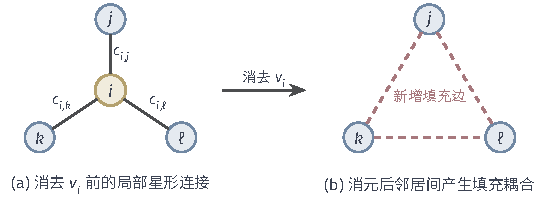
\includegraphics[width=92.385mm]{figures/03-graphs/05-matrices-and-spectra/tikz/electrical-cholesky-fill-in/figure.pdf}
  \caption{稀疏电网络直接消元中的填充现象。（a）消去顶点$i$之前，$i$与三个彼此不相邻的邻居$j,k,\ell$呈星形连接。（b）消去$v_i$后，邻居$j,k,\ell$之间两两产生新的非零耦合项（红色虚线填充边）。}
  \label{fig:electrical-cholesky-fill-in}
\end{BookInlineFigure}

\subsection{树上的线性时间求解}
\label{sec:electrical-tree-solve}

当电网络的正权支撑是一棵树$T=(V,E)$（边数$m=n-1$）时，图中不存在环路；按叶节点到根的顺序消元不会产生填充，任意消元顺序则未必如此。利用树的无环结构，无需显式构造矩阵，只需通过“自底向上求边电流、自顶向下求顶点电势”的两遍树遍历，就能在$O(n)$线性时间内精确解出拉普拉斯方程$\bm L\bm v=\bm b$。

先推导树上边电流与子树注入量的直接关系。任选顶点$q\in V$作为树的根（并令其为接地点$v_q=0$）。对每个非根顶点$i\neq q$，记$p(i)$为其父顶点，并将连接$i$与$p(i)$的唯一树边定向为从子指向父：$e_i\colon i\to p(i)$。删去树边$e_i$会将整棵树恰好切分为两部分：以$i$为根的子树$T_i$，以及包含根$q$的其余部分$V\setminus T_i$。

将子树$T_i$内部所有顶点$u\in T_i$的Kirchhoff电流守恒方程相加：子树内部的每一条边两个端点都在$T_i$内，其电流在尾端贡献正值、在头端贡献负值，正负成对抵消；唯一一条一端在$T_i$内、另一端在$T_i$外（即父顶点$p(i)$）的边界边正是$e_i\colon i\to p(i)$。因此，从$i$流向父顶点$p(i)$的边电流$s_i = f_{i\to p(i)}$必然精确等于整棵子树$T_i$内部的外部注入总和：
\begin{equation}
  s_i = \sum_{u\in T_i} b_u = b_i + \sum_{j\colon p(j) = i} s_j\qquad (i\neq q).
  \label{eq:electrical-subtree-injection}
\end{equation}

有了每条树边上的电流$s_i$后，再沿每条边$i\to p(i)$应用Ohm定律$s_i = c_{i,p(i)}(v_i - v_{p(i)})$，即可由父顶点的电势$v_{p(i)}$直接递推算出子顶点$i$的电势：
\begin{equation}
  v_i = v_{p(i)} + r_{i,p(i)}\,s_i\qquad (i\neq q),
  \label{eq:electrical-tree-voltage}
\end{equation}
其中$r_{i,p(i)} = 1/c_{i,p(i)}$为该树边的电阻。

据此，树上拉普拉斯方程$\bm L\bm v=\bm b$的$O(n)$求解算法完整流程如下（图~\ref{fig:electrical-tree-two-pass}）：

\paragraph{第一阶段：定根与父子序构建}
以接地点$q$为根，从$q$出发作一次广度优先或深度优先搜索，确定每个非根顶点$i\neq q$的父顶点$p(i)$及子节点列表，并按从根到叶的顺序记录遍历序列$(u_1=q, u_2, \ldots, u_n)$（父节点始终排在子节点之前）。

\paragraph{第二阶段：自底向上汇总子树注入求边电流（子节点先于父节点）}
按序列的逆序$u_n, u_{n-1}, \ldots, u_1$（即从叶子向根的自底向上顺序，此时处理顶点$i$时其所有子节点$j$的$s_j$均已算出）依次计算式~\eqref{eq:electrical-subtree-injection}：
\[
  s_i \leftarrow b_i + \sum_{j\colon p(j)=i} s_j.
\]
对叶节点，求和为空，直接有$s_i = b_i$；对内部节点$i\neq q$，算出的$s_i$即为边$i\to p(i)$上的电流。到达根节点$q$时，算出$s_q = \sum_{u\in V}b_u$：若$s_q\neq 0$，则外部注入总和不为零，报告方程组无解并终止；若$s_q = 0$，进入第三阶段。

\paragraph{第三阶段：自顶向下累加压降恢复顶点电势（父节点先于子节点）}
固定根节点电势$v_q \leftarrow 0$。按正序$u_2, \ldots, u_n$（即从根向叶的自顶向下顺序，此时处理顶点$i$时其父电势$v_{p(i)}$已经算出）依次由式~\eqref{eq:electrical-tree-voltage}计算
\[
  v_i \leftarrow v_{p(i)} + r_{i,p(i)}\,s_i.
\]
遍历结束即得全部顶点的唯一接地电势向量$\bm v$与全部树边的电流（若原边参考方向为$p(i)\to i$，只需将该边电流取为$-s_i$）。三个阶段均只对每个顶点和每条树边访问常数次，总时间复杂度和空间复杂度均为$O(n)$。

\begin{BookInlineFigure}
  \centering
  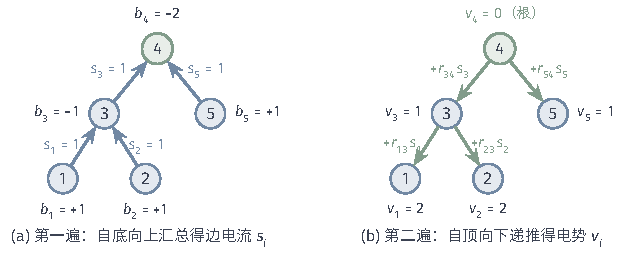
\includegraphics[width=105.174mm]{figures/03-graphs/05-matrices-and-spectra/tikz/electrical-tree-two-pass/figure.pdf}
  \caption{五顶点单位电阻树（以顶点$4$为根，注入$\bm b=(1,1,-1,-2,1)^\top$）上的两遍线性时间求解过程。（a）第一遍自底向上（从叶向根）按$s_i=b_i+\sum_{j:p(j)=i}s_j$汇总子树注入，直接定出每条边指向父节点的电流$s_1=1,s_2=1,s_3=-1+1+1=1,s_5=1$。（b）第二遍自顶向下（从根$v_4=0$向叶）按$v_i=v_{p(i)}+r_{i,p(i)}s_i$逐层累加压降，算出各点电势$v_3=1,v_5=1,v_1=2,v_2=2$。}
  \label{fig:electrical-tree-two-pass}
\end{BookInlineFigure}

以图~\ref{fig:electrical-tree-two-pass}中的五顶点单位电阻树（$r_e=1$）核对算法过程：设根为$4$，顶点$3$和$5$以$4$为父，叶子$1$和$2$以$3$为父，外部注入为$\bm b=(1,1,-1,-2,1)^\top$。

第一遍自底向上：叶子$1,2,5$直接取自身注入，得$s_1=1$、$s_2=1$、$s_5=1$；内部顶点$3$汇总自身注入$b_3=-1$与两个子节点的$s_1,s_2$，得$s_3 = -1 + 1 + 1 = 1$；根$4$处汇总得$s_4 = b_4 + s_3 + s_5 = -2 + 1 + 1 = 0$，守恒条件满足。

第二遍自顶向下：令根电势$v_4 = 0$；第一层子节点电势为$v_3 = v_4 + 1\times s_3 = 1$、$v_5 = v_4 + 1\times s_5 = 1$；第二层叶子电势为$v_1 = v_3 + 1\times s_1 = 2$、$v_2 = v_3 + 1\times s_2 = 2$，即得唯一接地电势解$\bm v=(2,2,1,0,1)^\top$。

\section{能量最小原理}
\label{sec:electrical-minimum-energy}

同样从顶点$1$送入一单位电流、从顶点$3$取出，可以有不同的分法。一种是把整股电流全部交给对角边，沿$1\to3$直走。另一种是让一半走对角边，另一半经过顶点$2$：先从$1$到$2$输送$1/2$，再从$2$到$3$输送$1/2$，对角边也输送$1/2$。两种分法在顶点$1$和$3$的净流出都是$1$和$-1$，在顶点$2$和$4$的净流出都是零——守恒条件满足得一样好。

哪种分法更优？我们比较两者的总耗散。一条边的耗散是电流乘压降。由Ohm定律，电阻为$r_e$的边上，压降为$r_e f_e$，耗散因此等于$r_e f_e^2$。电流翻一倍，耗散变成四倍。全网络的总耗散是各条边的贡献之和：
\begin{equation}
  \mathcal E(\bm f)
  = \sum_{e\in E} r_e f_e^2
  = \bm f^\top \bm C^{-1} \bm f.
  \label{eq:electrical-dissipation}
\end{equation}

四点图的边电阻都为一。全部走对角边时，只有一条边有电流$1$，耗散为$1^2 = 1$。一半走对角边、一半经顶点$2$时，三条边的电流各为$1/2$，耗散为$3 \times (1/2)^2 = 3/4$。分散在更多支路上，耗散反而更低了。

\paragraph{最小耗散定理}

那么在给定注入条件$\bm B\bm f = \bm b$下，哪种分法的耗散最小？答案正是上一节方程给出的实际电流。

\begin{theorem}[Thomson原理]
\label{thm:electrical-thomson}
设网络的边电导为正，各正权连通分量内的注入总量为零。对拉普拉斯方程的任一解$\bm v$，由Ohm定律得到的电流$\bm f_\star = \bm C\bm B^\top \bm v$是满足$\bm B\bm f = \bm b$的唯一最小耗散流。最小耗散为
\begin{equation}
  \mathcal E(\bm f_\star) = \bm b^\top \bm L^\dagger \bm b.
  \label{eq:electrical-minimum-dissipation}
\end{equation}
\end{theorem}

\begin{proof}
取任意另一组守恒流$\bm f$，记它与实际电流的差为$\bm z = \bm f - \bm f_\star$。两者满足同样的注入条件，因此差向量的净流出处处为零：$\bm B\bm z = \bm 0$。按第~\ref{chap:graph-incidence-matrix}章的术语，$\bm z$是一个环流。叠加环流改变各边的流量，但每个顶点的净流出保持原值。

将$\bm f = \bm f_\star + \bm z$代入总耗散并展开：
\[
  \mathcal E(\bm f_\star + \bm z)
  = \mathcal E(\bm f_\star) + \mathcal E(\bm z) + 2\bm f_\star^\top \bm C^{-1}\bm z.
\]
前两项分别是实际电流自身的耗散和附加环流自身的耗散。关键在于交叉项。

交叉项中，$\bm C^{-1}\bm f_\star$的第$e$项是$r_e f_{\star,e}$，也就是该边的压降$v_i - v_j$。所以
\[
  \bm f_\star^\top \bm C^{-1}\bm z
  = (\bm B^\top \bm v)^\top \bm z
  = \bm v^\top \bm B\bm z.
\]
第一个等号把每条边上的电阻乘电流换成电势差，第二个等号用到转置。由于$\bm B\bm z = \bm 0$，这个内积等于零。

直观地说，这是因为每个顶点$i$的贡献是$v_i \times (\bm B\bm z)_i = 0$。环流在每处进出相抵，电势无论取什么值都无法从中提取出功率。

去掉为零的交叉项后，
\begin{equation}
  \mathcal E(\bm f_\star + \bm z)
  = \mathcal E(\bm f_\star) + \mathcal E(\bm z).
  \label{eq:electrical-dissipation-decomposition}
\end{equation}
各边电阻为正，非零环流的耗散严格为正。因此任何不同于$\bm f_\star$的守恒流都有更大的耗散，极小流存在且唯一。

最后用顶点数据表示最小耗散。实际电流的耗散可以改写为
\[
  \mathcal E(\bm f_\star)
  = (\bm B^\top \bm v)^\top \bm C (\bm B^\top \bm v)
  = \bm v^\top \bm L\bm v.
\]
再用$\bm L\bm v = \bm b$，得到$\mathcal E(\bm f_\star) = \bm b^\top \bm v$。每个顶点的贡献是注入量乘电势：注入端电势高，取出端电势低，正注入乘正电势给出正的功率。

若某个分量的电势整体平移$c$，多出来的一项$c \cdot \bm 1^\top \bm b = 0$，所以耗散不依赖电势基准。取各分量内零均值的解$\bm v = \bm L^\dagger \bm b$，便得到式~\eqref{eq:electrical-minimum-dissipation}。
\end{proof}

这个结论称为\term{Thomson原理}（Thomson's principle）。

\paragraph{算例验证}

回到四点图的实际电流。四条环边各载$1/4$，耗散各为$(1/4)^2 = 1/16$。对角边载$1/2$，耗散为$(1/2)^2 = 1/4$。总耗散为$4 \times 1/16 + 1/4 = 1/2$。

现在取第~\ref{sec:incidence-cycle-space}节的基本环$\bm c_1$，它沿$1\to2\to3\to4\to1$的四条环边各送$1/4$个单位。叠加之后，看各条边的变化：

边$12$和$23$上原来各有$1/4$的电流，加上$1/4$变成$1/2$。

边$34$和$41$上原来各有$-1/4$的电流（实际从$4$流向$3$和从$1$流向$4$），加上$1/4$后恰好抵消为零。

对角边不在这个环上，仍然流过$1/2$。

这恰好就是本节开头的第二种分法：一半走对角边，一半经顶点$2$。由式~\eqref{eq:electrical-dissipation-decomposition}，附加环流使耗散增加$4 \times (1/4)^2 = 1/4$。已知实际耗散$1/2$，加上这一项得到$3/4$，与直接计算一致。

图~\ref{fig:electrical-distribution-dissipation}并排画出三种分流。(a)所有电流只走一条边，耗散为$1$。(b)分到两条路径后耗散降至$3/4$。(c)是网络自行选择的实际分流，耗散最低，为$1/2$。

\begin{BookInlineFigure}
  \centering
  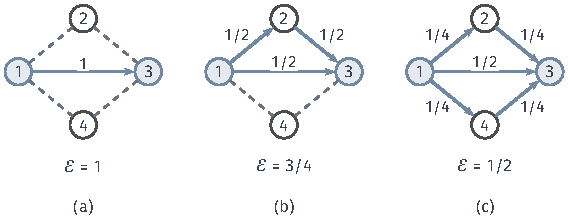
\includegraphics[scale=1]{figures/03-graphs/05-matrices-and-spectra/tikz/electrical-distribution-dissipation/figure.pdf}
  \caption{同一单位注入下的三种分流。顶点$1$注入一单位电流，顶点$3$引出一单位，各边电阻都为一。箭头和数值给出有流量的边，虚线为零电流的边。(a)~只走对角边，(b)~平分到对角边和上路，(c)~网络的实际分流。}
  \label{fig:electrical-distribution-dissipation}
\end{BookInlineFigure}

\paragraph{与最小费用流的比较}

第~\ref{chap:min-cost-flow}章的最小费用流也在守恒条件下选流量，但目标函数是线性的，通常还有容量约束。这里的耗散是严格凸的二次函数，不存在容量限制，边流可以取任意实数。正因为严格凸，极小点唯一——不需要另外检查是否有多个最优解。即使注入量为整数，最优的边流量也可能是分数，如本例中的$1/4$和$1/2$。

\section{有效电阻}
\label{sec:graph-effective-resistance}

从外部观察一个电网络时，如果只在两个选定端点$a$和$b$之间接入一单位电流并测量这两点之间的电势差，网络内部复杂的串并联与环路分流就被浓缩为一个标量——两点之间的有效电阻。本节依次介绍有效电阻的定义与三种等价表达、不同复杂度网络上有效电阻的精确计算方法、大规模网络上有效电阻的三种近似计算方法，以及有效电阻作为图上距离度量的基本性质。

\subsection{有效电阻的定义}
\label{sec:electrical-resistance-definition}

单条电阻为$r$的边在通过$1$单位电流时产生压降$r$。把这一测量方式推广到整张网络中的任意一对顶点$a,b$，就得到有效电阻的定义。

\begin{definition}[有效电阻]
\label{def:graph-effective-resistance}
设$a,b$是同一正权连通分量中的两个不同顶点。取单位偶极注入向量$\bm b_{a,b} = \bm e_a - \bm e_b$（即在顶点$a$注入$1$单位电流、从顶点$b$引出$1$单位电流，其余顶点注入为零）。设$\bm v\in\mathbb R^n$为拉普拉斯方程$\bm L\bm v = \bm b_{a,b}$的任一电势解，定义顶点$a$与$b$之间的\term{有效电阻}（effective resistance）为
\begin{equation}
  R_{a,b} = v_a - v_b.
  \label{eq:electrical-resistance-definition}
\end{equation}
此外，约定同一点的有效电阻为$R_{a,a} = 0$；若$a,b$分属不同的正权连通分量，约定$R_{a,b} = +\infty$。
\end{definition}

由定理~\ref{thm:electrical-laplacian-solvability}(2)，不同电势解在每个正权连通分量上分别相差一个常数；对包含$a,b$的分量记这一常数为$c$，相减后$(v_a+c)-(v_b+c)=v_a-v_b$，故定义~\ref{def:graph-effective-resistance}完全不依赖接地点的选取。若将注入电流从$1$单位改为任意$I$单位（即右端取$I\bm b_{a,b}$），由方程的线性性，两端电势差变为$v_a - v_b = I\cdot R_{a,b}$，说明整张网络对外部端点$a,b$的端口响应完全等价于在$a,b$之间单独连接一个阻值为$R_{a,b}$的电阻器。

除了定义式~\eqref{eq:electrical-resistance-definition}外，有效电阻还有两种常用的等价代数与变分表达：

第一种是\emph{伪逆二次型表达}。在连通分量上取零均值电势解$\bm v = \bm L^\dagger \bm b_{a,b}$，由于$v_a - v_b = (\bm e_a - \bm e_b)^\top\bm v = \bm b_{a,b}^\top\bm v$，代入即得
\begin{equation}
  R_{a,b}
  = \bm b_{a,b}^\top \bm L^\dagger \bm b_{a,b}
  = (\bm e_a - \bm e_b)^\top \bm L^\dagger (\bm e_a - \bm e_b)
  = L^\dagger_{a,a} + L^\dagger_{b,b} - 2L^\dagger_{a,b}.
  \label{eq:electrical-resistance-pseudoinverse}
\end{equation}

第二种是\emph{Thomson最小耗散表达}。在定理~\ref{thm:electrical-thomson}的式~\eqref{eq:electrical-minimum-dissipation}中取$\bm b = \bm b_{a,b} = \bm e_a - \bm e_b$，最小总耗散为$\bm b_{a,b}^\top\bm L^\dagger\bm b_{a,b} = v_a - v_b = R_{a,b}$，因此有效电阻恰好等于从$a$向$b$输送$1$单位守恒流所需的最小总耗散：
\begin{equation}
  R_{a,b} = \min_{\bm B\bm f = \bm e_a - \bm e_b} \bm f^\top \bm C^{-1} \bm f.
  \label{eq:electrical-resistance-energy}
\end{equation}
式~\eqref{eq:electrical-resistance-pseudoinverse}便于通过线性代数直接计算单对或多对顶点的有效电阻；式~\eqref{eq:electrical-resistance-energy}则便于分析网络结构变化（如添边或增大电导）对有效电阻的单调影响。

\subsection{有效电阻的计算}
\label{sec:electrical-series-parallel}

针对结构复杂度不同的电网络，可以按由简入繁的顺序选用三种精确计算方法：对串并联简单结构直接作局部归约；对含桥式结构的小规模网络考虑星-三角（$\text{Y--}\Delta$）变换；对一般中等规模网络直接求解接地拉普拉斯线性方程组。

\subsubsection{简单结构：串联、并联与悬空支路}
\label{sec:electrical-simple-reductions}

当网络局部只包含串联路径、并联重边或无源悬空支路时，可以逐步将局部子网替换为单条等效边，同时保持端口的电势差与电流关系不变。

\paragraph{串联归约}
设两条边$e_1=\{u,w\}$与$e_2=\{w,v\}$在内部顶点$w$处首尾相接，且中间顶点$w$的度数为$2$、没有外部电流注入（$b_w=0$）。此时Kirchhoff电流定律要求流过两条边的电流大小完全相同，记为$I$。两段边上的压降分别为$I r_1$与$I r_2$，从$u$到$v$的总压降为$I(r_1 + r_2)$，因此可将两条串联边合并为一条连接$u,v$的等效边，其等效电阻等于两段电阻之和：
\begin{equation}
  r_{\mathrm{series}} = r_1 + r_2, \qquad
  c_{\mathrm{series}} = \frac{c_1 c_2}{c_1 + c_2}.
  \label{eq:electrical-series}
\end{equation}
需要注意，若中间顶点$w$还连接着第三条边或有外部电流注入，流过两段的电流一般不同，不能直接套用串联公式。

\paragraph{并联归约}
设连接同一对端点$u,v$的多条支路具有电导$c_1,c_2,\ldots,c_k$。由于它们共用相同的两端压降$\Delta v = v_u - v_v$，第$i$条支路流过的电流为$c_i\Delta v$，总电流为$\bigl(\sum_i c_i\bigr)\Delta v$。因此可将多条并联支路合并为一条等效边，其等效电导等于各支路电导之和（等效电阻为总电导的倒数）：
\begin{equation}
  c_{\mathrm{parallel}} = \sum_i c_i, \qquad
  r_{\mathrm{parallel}} = \left(\sum_i \frac{1}{r_i}\right)^{-1}.
  \label{eq:electrical-parallel}
\end{equation}
此外，若网络中存在不包含查询端点$a,b$的悬空叶节点（度为$1$且无外部注入），由电流守恒知该悬空边上的电流必为零，可直接将其删去而不影响$R_{a,b}$。

\begin{BookInlineFigure}
  \centering
  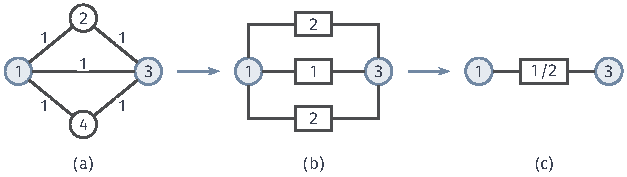
\includegraphics[scale=1]{figures/03-graphs/05-matrices-and-spectra/tikz/electrical-series-parallel-reduction/figure.pdf}
  \caption{四点网络在端点$1,3$之间的串并联简化。数字是边或支路的电阻。(a)~五条单位电阻边，(b)~分别合并经过顶点$2$和顶点$4$的两组串联边，得到阻值为$2,1,2$的三条并联支路，(c)~再合并为阻值$1/2$的单条边。}
  \label{fig:electrical-series-parallel-reduction}
\end{BookInlineFigure}

以四点五边单位电阻图（每条边$r_e=1$）计算$R_{1,3}$为例（图~\ref{fig:electrical-series-parallel-reduction}）。当查询端点为$1$和$3$时，中间顶点$2$和$4$的度数均为$2$且无外部注入：

第一步，作串联归约（图~\ref{fig:electrical-series-parallel-reduction}(b)）。经过顶点$2$的两条边$12,23$串联，合并为连接$1,3$、阻值为$1+1=2$（电导$1/2$）的上支路；经过顶点$4$的两条边$14,43$同样串联，合并为阻值为$1+1=2$（电导$1/2$）的下支路。

第二步，作并联归约（图~\ref{fig:electrical-series-parallel-reduction}(c)）。现在端点$1,3$之间共有三条并联支路，电阻分别为$2,1,2$，电导分别为$1/2,1,1/2$。将三者电导相加得总电导$c_{\mathrm{parallel}} = 1/2 + 1 + 1/2 = 2$，取倒数立得
\[
  R_{1,3} = \frac{1}{1/2 + 1 + 1/2} = \frac{1}{2},
\]
与例~\ref{ex:electrical-four-vertex-network}通过解方程算出的$v_1 - v_3 = 1/2 - 0 = 1/2$完全一致。

\subsubsection{小规模桥式结构：星-三角变换}
\label{sec:electrical-wye-delta}

单纯依靠串联和并联归约并不能化简所有双端网络。例如在四点环加对角边$13$的五边图上，以$2,4$为查询端点时，两个内部顶点$1,3$的度数都为$3$，既没有可消去的二度无源顶点，也没有平行重边。这是一个桥式结构；若各臂阻值恰好平衡，还可另用对称性化简，但一般边权下不能作此假设。

对于度为$3$的内部接点，可用\emph{星-三角变换}（$\text{Y--}\Delta$ transformation）：把以无源顶点$w$为中心的三条星形支路替换为三个外围顶点之间的三角形支路，或反向操作，同时保持端口电势与电流关系（图~\ref{fig:electrical-wye-delta-bridge}(a)）。下文选取仍可串并联化简的$R_{1,2}$作为计算示例，以便交叉核验变换结果。

\begin{theorem}[星-三角（$\text{Y--}\Delta$）等效变换]
\label{thm:electrical-wye-delta}
设中心顶点$w$不接入外部电流（$b_w=0$），且仅与三个外围顶点$u_1,u_2,u_3$相连，三条星形支路的电导分别为$c_1,c_2,c_3>0$（对应电阻为$r_1,r_2,r_3$）。消去中心顶点$w$后，该星形子网对$u_1,u_2,u_3$的端口电势与电流关系，完全等价于在$u_1,u_2,u_3$之间两两连接一条三角形边，其中连接$u_i$与$u_j$（$1\leq i<j\leq 3$，记第三个下标为$k$）的等效电导$c_{i,j}$与等效电阻$r_{i,j}$分别为
\begin{equation}
  c_{i,j} = \frac{c_i c_j}{c_1 + c_2 + c_3}, \qquad
  r_{i,j} = \frac{r_1 r_2 + r_2 r_3 + r_3 r_1}{r_k}.
  \label{eq:electrical-y-to-delta}
\end{equation}
反之，若已知$u_1,u_2,u_3$之间的三角形边电阻为$r_{1,2},r_{2,3},r_{3,1}>0$，将其等价变换为以新增无源顶点$w$为中心的星形支路（$\Delta\to\text{Y}$变换）时，连接$u_i$与$w$的星形支路电阻为
\begin{equation}
  r_i = \frac{r_{i,j}\,r_{i,k}}{r_{1,2} + r_{2,3} + r_{3,1}} \qquad (\{i,j,k\}=\{1,2,3\}).
  \label{eq:electrical-delta-to-y}
\end{equation}
\end{theorem}

\begin{proof}
在星形网络中，中心顶点$w$无外部注入（$b_w=0$），其Kirchhoff电流守恒方程为
\[
  (c_1 + c_2 + c_3)v_w - (c_1 v_1 + c_2 v_2 + c_3 v_3) = 0,
\]
解出中心电势为外围三点电势的加权平均：
\[
  v_w = \frac{c_1 v_1 + c_2 v_2 + c_3 v_3}{c_1 + c_2 + c_3}.
\]

将$v_w$代入外围顶点$u_1$从星形子网流出的电流$I_1 = c_1(v_1 - v_w)$，通分整理得
\[
  \begin{aligned}
    I_1
    &= c_1\left(v_1 - \frac{c_1 v_1 + c_2 v_2 + c_3 v_3}{c_1 + c_2 + c_3}\right)\\
    &= \frac{c_1 c_2}{c_1 + c_2 + c_3}(v_1 - v_2) + \frac{c_1 c_3}{c_1 + c_2 + c_3}(v_1 - v_3).
  \end{aligned}
\]
对$u_2$和$u_3$同理。这恰与在$u_i,u_j$之间连接电导为$c_{i,j} = \frac{c_i c_j}{c_1+c_2+c_3}$的三角形边所产生的端口电流完全相同。将$c_i = 1/r_i$代入$r_{i,j}=1/c_{i,j}$并上下同乘$r_1 r_2 r_3$，即得式~\eqref{eq:electrical-y-to-delta}的第二式；求解式~\eqref{eq:electrical-y-to-delta}关于$r_1,r_2,r_3$的代数反演即得$\Delta\to\text{Y}$公式~\eqref{eq:electrical-delta-to-y}。
\end{proof}

\begin{BookInlineFigure}
  \centering
  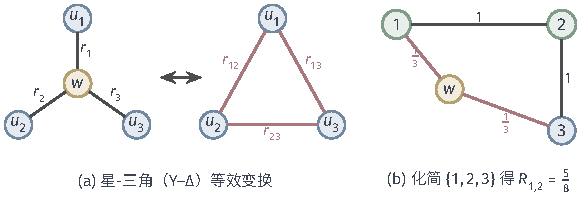
\includegraphics[width=98.591mm]{figures/03-graphs/05-matrices-and-spectra/tikz/electrical-wye-delta-bridge/figure.pdf}
  \caption{星-三角（$\text{Y--}\Delta$）变换及其在桥式结构化简中的应用。（a）无源中心顶点$w$的星形三支路与外围三角形三支路相互等效。（b）计算四点五边图的$R_{1,2}$时，将左下三角形$\{1,3,4\}$通过$\Delta\to\text{Y}$变换化为中心顶点$w$的星形（有效支路电阻为$1/3$），再由串并联算出$R_{1,2}=5/8$。}
  \label{fig:electrical-wye-delta-bridge}
\end{BookInlineFigure}

下面在四点五边单位电阻图上演示如何用星-三角变换求出$R_{1,2}$（图~\ref{fig:electrical-wye-delta-bridge}(b)）。在图$\mathcal G$中，顶点$1,2,3$构成右上三角形，顶点$1,3,4$构成左下三角形：

第一步，对左下角的单位电阻三角形$\{1,3,4\}$（三条边电阻均为$1$）施行$\Delta\to\text{Y}$变换~\eqref{eq:electrical-delta-to-y}。引入星形中心$w$替换该三角形后，连接$1,3,4$的三条星形支路电阻均为
\[
  r_1 = r_3 = r_4 = \frac{1\times 1}{1 + 1 + 1} = \frac{1}{3}.
\]
由于顶点$4$不是查询端点（无外部注入），变换后悬挂在$w$上的支路$w\!-\!4$成为无源悬空叶边，电流为零，直接删去（见图~\ref{fig:electrical-wye-delta-bridge}(b)）。

第二步，对剩余的串并联支路直接求值。在图~\ref{fig:electrical-wye-delta-bridge}(b)中，从端点$1$到端点$2$现在只剩两条并联支路：一条是上方的直接边$1\!-\!2$（电阻为$1$）；另一条依次经过$1\to w\to 3\to 2$，由三段串联组成，总电阻为
\[
  r_{1\to w\to 3\to 2} = \frac{1}{3} + \frac{1}{3} + 1 = \frac{5}{3}.
\]
将阻值为$1$和$5/3$的两条支路并联，立得
\[
  R_{1,2} = \frac{1 \times \frac53}{1 + \frac53} = \frac{5}{8}.
\]

\subsubsection{中等规模网络：求解拉普拉斯方程}
\label{sec:electrical-medium-laplacian-solve}

当网络规模达到数十至数万个顶点、内部包含大量交错环路时，手工寻找星-三角变换和串并联归约不再现实。此时最通用、系统的计算方法是直接回到定义~\ref{def:graph-effective-resistance}：固定端点$b$接地（令$v_b = 0$），在端点$a$注入$1$单位电流，求解$(n-1)\times(n-1)$对称正定线性方程组
\[
  \overline{\bm L}\,\overline{\bm v} = \overline{\bm e}_a,
\]
解出电势后直接读取顶点$a$处的电势值，即有$R_{a,b} = v_a - v_b = v_a$。若需要查询多对顶点之间的有效电阻，可先对$\overline{\bm L}$作一次Cholesky分解（或求出伪逆$\bm L^\dagger$），再利用式~\eqref{eq:electrical-resistance-pseudoinverse}计算$R_{a,b} = L^\dagger_{a,a} + L^\dagger_{b,b} - 2L^\dagger_{a,b}$。

下面用求解拉普拉斯方程的方法重新计算四点五边单位电阻图上的$R_{1,2}$（图~\ref{fig:electrical-r12-potential-flow}），与上一小节的星-三角化简结果核对。设从顶点$1$注入$1$单位电流、从顶点$2$引出$1$单位电流，令顶点$2$接地（$v_2 = 0$）：

第一步，利用无源顶点$4$的守恒方程消去$v_4$。顶点$4$无外部注入，连接邻居$1$和$3$，度为$2$，故
\[
  2v_4 - v_1 - v_3 = 0 \quad\Longrightarrow\quad v_4 = \frac{v_1 + v_3}{2}.
\]

第二步，利用无源顶点$3$的守恒方程求出$v_3$与$v_1$的比例关系。顶点$3$无外部注入，连接邻居$1,2,4$，度为$3$，故
\[
  3v_3 - v_1 - v_2 - v_4 = 0.
\]
将$v_2 = 0$和$v_4 = (v_1 + v_3)/2$代入上式，化简得$5v_3 = 3v_1$，即
\[
  v_3 = \frac{3}{5}v_1, \qquad v_4 = \frac{1}{2}\Bigl(v_1 + \frac{3}{5}v_1\Bigr) = \frac{4}{5}v_1.
\]

第三步，代入注入端顶点$1$的守恒方程解出$v_1$。顶点$1$连接邻居$2,3,4$，度为$3$，外部注入为$1$，故
\[
  3v_1 - v_2 - v_3 - v_4 = 1.
\]
代入$v_2 = 0$、$v_3 = \frac35 v_1$、$v_4 = \frac45 v_1$，得
\[
  3v_1 - 0 - \frac{3}{5}v_1 - \frac{4}{5}v_1 = \frac{8}{5}v_1 = 1
  \quad\Longrightarrow\quad v_1 = \frac{5}{8}.
\]
由此得到全部顶点的接地电势向量为
\[
  \bm v = \Bigl(\frac{5}{8}, \; 0, \; \frac{3}{8}, \; \frac{1}{2}\Bigr)^\top,
\]
两端有效电阻为$R_{1,2} = v_1 - v_2 = 5/8$，与星-三角变换算出的结果完全一致。

\begin{BookInlineFigure}
  \centering
  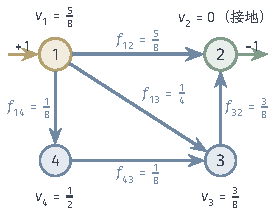
\includegraphics[width=46.718mm]{figures/03-graphs/05-matrices-and-spectra/tikz/electrical-r12-potential-flow/figure.pdf}
  \caption{在四点单位电阻网络中求解$\bm L\bm v=\bm e_1-\bm e_2$（令$v_2=0$接地）计算有效电阻$R_{1,2}=5/8$。顶点旁标注电势值，边上箭头与数字标出五条边的实际分流大小：直接边$1\to 2$承载$5/8$，经由$1\to 3\to 2$和$1\to 4\to 3\to 2$的旁路合流$1/4+1/8=3/8$注入终点$2$。}
  \label{fig:electrical-r12-potential-flow}
\end{BookInlineFigure}

对比$R_{1,2} = 5/8$与$R_{1,3} = 1/2$可以发现：虽然顶点对$(1,2)$和$(1,3)$之间都有一条单位电阻的边直接相连，但$(1,3)$之间有两条对称的二步旁路分担电流，而$(1,2)$之间的旁路需要绕行更远的路径，因此$R_{1,2} > R_{1,3}$。有效电阻综合反映了整张网络在两点之间提供的全体并行通路容量，而不仅仅是直接相连边的电阻。

\subsection{有效电阻的近似计算}
\label{sec:electrical-approximate-resistance}

在包含百万级顶点和边的大规模图（例如社交网络、道路网或第~\ref{chap:graph-sparsification}章的图稀疏化问题，其中需要求出全部$m$条边两端点的有效电阻）上，若直接按定义对每条边求解一次拉普拉斯线性系统，总共需要求解$m$次方程。若每次求解的成本为$T_{\mathrm{solve}}$，这部分总成本为$O(mT_{\mathrm{solve}})$，因所用求解器、精度和预处理复用方式而异。为此，本小节介绍大规模图上批量或快速近似计算有效电阻的三种常见方法：欧氏嵌入与随机投影降维法、谱展开与低频主模态截断法，以及基于随机游走与生成树的蒙特卡洛采样法。

\subsubsection{欧氏嵌入与随机投影降维}
\label{sec:electrical-resistance-embedding}
\label{sec:electrical-resistance-jl}
\label{sec:electrical-resistance-solver-error}

第一种方法是Spielman与Srivastava提出的随机投影法\scite{spielman2011graph}，它将全部点对的有效电阻转化为低维欧氏空间中的两点距离平方，使全图所有边的有效电阻只需通过求解$k=O(\varepsilon^{-2}\log n)$个拉普拉斯线性系统即可在高概率下获得$(1\pm\varepsilon)$相对精度的批量估计，前提是线性求解误差也得到控制。该方法分三步实现：

\paragraph{第一步：精确欧氏嵌入}
设网络连通。从顶点$a$向$b$注入$1$单位电流时，零均值电势解为$\bm u = \bm L^\dagger \bm b_{a,b}$，每条边$e$上的耗散为$c_e\bigl((\bm B^\top\bm u)_e\bigr)^2 = \bigl((\bm C^{1/2}\bm B^\top\bm L^\dagger\bm b_{a,b})_e\bigr)^2$。将“求零均值电势$\bm L^\dagger$—取沿边差分$\bm B^\top$—按$\sqrt{c_e}$缩放$\bm C^{1/2}$”合成为一个$m\times n$矩阵：
\begin{equation}
  \bm Z = \bm C^{1/2} \bm B^\top \bm L^\dagger \in \mathbb R^{m \times n}.
  \label{eq:electrical-resistance-embedding}
\end{equation}
矩阵$\bm Z$的第$a$列$\bm Z\bm e_a\in\mathbb R^m$即为顶点$a$的$m$维精确嵌入坐标。利用$\bm L=\bm B\bm C\bm B^\top$以及伪逆恒等式$\bm L^\dagger\bm L\bm L^\dagger=\bm L^\dagger$，有
\[
  \bm Z^\top \bm Z
  = \bm L^\dagger \bm B\bm C \bm B^\top \bm L^\dagger
  = \bm L^\dagger \bm L \bm L^\dagger
  = \bm L^\dagger.
\]
因此，任意两个顶点$a,b$之间的有效电阻精确等于它们在$\bm Z$中对应坐标列之差的欧氏长度平方：
\[
  \lVert \bm Z(\bm e_a-\bm e_b) \rVert_2^2
  = \bm b_{a,b}^\top \bm Z^\top \bm Z\bm b_{a,b}
  = \bm b_{a,b}^\top \bm L^\dagger \bm b_{a,b}
  = R_{a,b}.
\]

在四点单位权图上核对：从$1$到$3$单位注入的零均值电势为$(1/4, 0, -1/4, 0)^\top$，沿五条边取差得
\[
  \bm Z(\bm e_1 - \bm e_3) = (1/4, \; 1/4, \; -1/4, \; -1/4, \; 1/2)^\top,
\]
五项平方和为$4\times(1/4)^2+(1/2)^2=1/2=R_{1,3}$；同理，对顶点$1,2$，精确列差向量为
\[
  \bm Z(\bm e_1 - \bm e_2) = (5/8, \; -3/8, \; -1/8, \; -1/8, \; 1/4)^\top,
\]
其欧氏长度平方为$25/64+9/64+1/64+1/64+4/64=40/64=5/8=R_{1,2}$。

\paragraph{第二步：随机投影降维与$k$次线性求解}
由于$m$维嵌入矩阵$\bm Z\in\mathbb R^{m\times n}$维数过高，引入一个元素独立同分布于$\mathcal N(0,1/k)$（或$\pm 1/\sqrt{k}$ Rademacher分布）的$k\times m$随机投影矩阵$\bm Q \in \mathbb R^{k \times m}$（$k\ll m$），将所有顶点的坐标列线性压缩为$k\times n$低维坐标矩阵$\bm Y = \bm Q\bm Z$，并用低维坐标差的欧氏长度平方估计有效电阻：
\[
  \widehat R_{a,b} = \lVert \bm Y(\bm e_a - \bm e_b) \rVert_2^2.
\]

计算$\bm Y=\bm Q\bm Z$无需先算出$\bm L^\dagger$或$\bm Z$。记$\bm q_j^\top\in\mathbb R^{1\times m}$为$\bm Q$的第$j$行（$j=1,\ldots,k$），先计算零和右端向量$\bm d_j = \bm B\bm C^{1/2} \bm q_j\in\bm 1^\perp$，然后求解拉普拉斯方程并取零均值解：
\begin{equation}
  \bm L\bm y_j = \bm d_j, \qquad \bm 1^\top \bm y_j = 0.
  \label{eq:electrical-projection-systems}
\end{equation}
由于$\bm y_j = \bm L^\dagger \bm d_j=\bm L^\dagger\bm B\bm C^{1/2}\bm q_j$且$\bm L^\dagger$对称，转置后即得$\bm y_j^\top = \bm q_j^\top \bm C^{1/2} \bm B^\top \bm L^\dagger = \bm q_j^\top \bm Z$，这正是$\bm Y$的第$j$行。因此，只需对$k$个随机右端各求解一次拉普拉斯系统即可得到全部顶点的$k$维坐标$\bm Y$，此后查询任意一对顶点的有效电阻仅需$O(k)$时间。

以四点单位权图演示$k = 3$的投影计算过程（图~\ref{fig:electrical-resistance-coordinate-projection}）。使用随机数种子\texttt{random.Random(17)}按行生成标准正态随机数并除以$\sqrt{3}$得到$3\times 5$矩阵$\bm Q$，其第一行为$\bm q_1^\top\approx(-1.0368, -0.1441, 0.4628, -0.1173, 0.0910)$；左乘$\bm B\bm C^{1/2}$得$\bm d_1 \approx (-0.8284, 0.8926, 0.5159, -0.5801)^\top$，解出零均值电势即得$\bm Y$的第一行$\bm y_1^\top \approx (-0.2071, 0.4073, 0.1290, -0.3291)$。同样解出第二、第三行后，取$\bm Y$中第$1$列与第$3$列之差的平方和即得估计值$\widehat R_{1,3}\approx 0.3680$，第$1$列与第$2$列之差的平方和给出$\widehat R_{1,2}\approx 0.8263$。

\begin{BookInlineFigure}
  \centering
  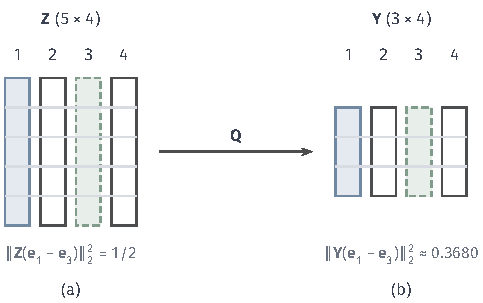
\includegraphics[scale=1]{figures/03-graphs/05-matrices-and-spectra/tikz/electrical-resistance-coordinate-projection/figure.pdf}
  \caption{用两列坐标的欧氏距离平方查询四点图中顶点$1,3$之间的有效电阻。蓝色实框和绿色虚框分别标出顶点$1$和$3$的坐标列。(a)~五维精确坐标$\bm Z$给出$R_{1,3}=1/2$。(b)~左乘随机矩阵$\bm Q$压缩为三维坐标$\bm Y=\bm Q\bm Z$后取列差平方和。}
  \label{fig:electrical-resistance-coordinate-projection}
\end{BookInlineFigure}

下面的定理利用\term{Johnson--Lindenstrauss引理}（Johnson--Lindenstrauss lemma）证明，只需取$k=O(\varepsilon^{-2}\log n)$，就能以高概率同时保证全图所有顶点对的相对误差不超过$\varepsilon$。

\begin{theorem}[高斯投影保留电阻距离]
\label{thm:electrical-jl-resistance}
设$n \geq 2$且正权网络连通，给定相对误差参数$0 < \varepsilon < 1$与失败概率上限$0 < \delta < 1$。令$\bm Q\in\mathbb R^{k\times m}$的元素独立同分布于均值为$0$、方差为$1/k$的正态分布$\mathcal N(0,1/k)$。若投影维数满足
\begin{equation}
  k \geq \frac{8}{\varepsilon^2}\log\frac{n(n-1)}{\delta},
  \label{eq:electrical-projection-dimension}
\end{equation}
则以至少$1 - \delta$的概率，所有顶点对$a,b\in V$同时满足
\begin{equation}
  (1 - \varepsilon)\,R_{a,b}
  \leq \lVert \bm Q\bm Z(\bm e_a - \bm e_b) \rVert_2^2
  \leq (1 + \varepsilon)\,R_{a,b}.
  \label{eq:electrical-projection-guarantee}
\end{equation}
\end{theorem}

\begin{proof}
第一步，分析单个固定非零向量$\bm z\in\mathbb R^m$投影后的分布。由于$\bm Q$的各行独立且元素服从$\mathcal N(0,1/k)$，$\bm Q\bm z$的$k$个分量相互独立且均服从$\mathcal N(0,\lVert\bm z\rVert_2^2/k)$。将各分量除以标准差$\lVert\bm z\rVert_2/\sqrt{k}$后求平方和，所得随机变量
\[
  X = \frac{k\,\lVert\bm Q\bm z\rVert_2^2}{\lVert\bm z\rVert_2^2}=\sum_{j=1}^k \xi_j^2\qquad\bigl(\xi_j\stackrel{\mathrm{i.i.d.}}{\sim}\mathcal N(0,1)\bigr)
\]
服从自由度为$k$的卡方分布，其矩母函数为$\mathbb E[\exp(tX)] = (1 - 2t)^{-k/2}$（$t<1/2$）。

第二步，用Chernoff界估计上下尾概率。对上尾事件$X \geq k(1 + \varepsilon)$，取$t = \varepsilon/[2(1 + \varepsilon)]\in(0,1/2)$应用Markov不等式，得
\[
  \mathbb P\bigl(X \geq k(1 + \varepsilon)\bigr)
  \leq \exp\bigl(-tk(1 + \varepsilon)\bigr)\,(1 - 2t)^{-k/2}
  = \exp\!\left(-\frac{k}{2}\bigl(\varepsilon - \log(1 + \varepsilon)\bigr)\right).
\]
对下尾事件$X \leq k(1 - \varepsilon)$，取$t = -\varepsilon/[2(1 - \varepsilon)] < 0$应用Markov不等式，得
\[
  \mathbb P\bigl(X \leq k(1 - \varepsilon)\bigr)
  \leq \exp\!\left(-\frac{k}{2}\bigl(-\varepsilon - \log(1 - \varepsilon)\bigr)\right).
\]
对$0 < \varepsilon < 1$，利用不等式$\varepsilon-\log(1+\varepsilon)\geq\varepsilon^2/4$和$-\varepsilon-\log(1-\varepsilon)\geq\varepsilon^2/2>\varepsilon^2/4$，合并上下尾可知单个向量$\bm z$的投影长度平方偏离$(1 \pm \varepsilon)\lVert\bm z\rVert_2^2$的概率至多为$2\exp(-k\varepsilon^2/8)$。

第三步，对全部顶点对应用联合界。图中不同顶点的无序对$\{a,b\}$共有$\binom{n}{2}=n(n-1)/2$对，每对对应$\bm z=\bm Z(\bm e_a - \bm e_b)$（长度平方为$R_{a,b}$）。由布尔不等式，至少有一对超出式~\eqref{eq:electrical-projection-guarantee}的概率至多为
\[
  \frac{n(n-1)}{2}\cdot 2\exp\!\left(-\frac{k\varepsilon^2}{8}\right)=n(n-1)\exp\!\left(-\frac{k\varepsilon^2}{8}\right).
\]
当$k$满足式~\eqref{eq:electrical-projection-dimension}时，该概率上界不超过$\delta$。
\end{proof}

\paragraph{第三步：迭代求解的误差控制}
用共轭梯度法近似求解式~\eqref{eq:electrical-projection-systems}的$k$个方程时，设第$j$个方程的近似零均值解为$\widetilde{\bm y}_j$，误差为$\bm h_j = \widetilde{\bm y}_j - \bm y_j$。记单位注入的精确电势为$\bm u = \bm L^\dagger \bm b_{a,b}$，由$\bm L\bm u = \bm b_{a,b}$及能量内积的Cauchy--Schwarz不等式，第$j$行坐标差的误差满足
\[
  |\bm h_j^\top \bm b_{a,b}|
  = |\bm h_j^\top \bm L\bm u|
  \leq \lVert\bm h_j\rVert_{\bm L}\,\lVert\bm u\rVert_{\bm L}
  = \lVert\bm h_j\rVert_{\bm L}\,\sqrt{R_{a,b}}.
\]
若将全部$k$次求解的总能量误差控制在$\sum_{j=1}^k \lVert\bm h_j\rVert_{\bm L}^2 \leq \eta^2$以内，则$\lVert(\widetilde{\bm Y}-\bm Y)\bm b_{a,b}\rVert_2\leq\eta\sqrt{R_{a,b}}$。结合式~\eqref{eq:electrical-projection-guarantee}与三角不等式，对$a\ne b$，最终估计值$\widehat R_{a,b} = \lVert \widetilde{\bm Y}\bm b_{a,b}\rVert_2^2$满足
\begin{equation}
  \max\{0, \sqrt{1-\varepsilon} - \eta\}
  \leq \sqrt{\frac{\widehat R_{a,b}}{R_{a,b}}}
  \leq \sqrt{1+\varepsilon} + \eta.
  \label{eq:electrical-resistance-total-error}
\end{equation}

\subsubsection{谱展开与低频主模态截断}
\label{sec:electrical-resistance-spectral-truncation}

第二种常见方法利用拉普拉斯矩阵的正交谱分解。在连通图上，设$\bm L$的特征值为$0=\lambda_1<\lambda_2\leq\cdots\leq\lambda_n$，对应的标准正交特征向量为$\bm u_1,\bm u_2,\ldots,\bm u_n$（其中$\bm u_1=\frac{1}{\sqrt n}\bm 1$）。由伪逆的谱分解
\[
  \bm L^\dagger = \sum_{i=2}^n \frac{1}{\lambda_i}\bm u_i\bm u_i^\top,
\]
将其代入式~\eqref{eq:electrical-resistance-pseudoinverse}，可得有效电阻的\emph{谱展开公式}：
\begin{equation}
  R_{a,b}
  = (\bm e_a - \bm e_b)^\top\bm L^\dagger(\bm e_a - \bm e_b)
  = \sum_{i=2}^n \frac{1}{\lambda_i}(u_{i,a} - u_{i,b})^2.
  \label{eq:electrical-resistance-spectral-sum}
\end{equation}

在式~\eqref{eq:electrical-resistance-spectral-sum}中，每个正交模态的贡献被特征值的倒数$1/\lambda_i$加权：较小的非零特征值（低频全局模态）权重$1/\lambda_i$最大，但单对顶点上的实际贡献还取决于坐标差$(u_{i,a}-u_{i,b})^2$，不能只据特征值断定低频项占主导；而较大的特征值（高频局部振荡模态）权重$1/\lambda_i$较小。当已通过Lanczos方法预先求出前$r$个最小非零特征对$(\lambda_i,\bm u_i)$（$i=2,\ldots,r+1$，$r\ll n$）时，只保留前$r$项即可构造低秩谱截断近似：
\[
  R_{a,b}^{(r)} = \sum_{i=2}^{r+1}\frac{1}{\lambda_i}(u_{i,a} - u_{i,b})^2.
\]
由于被截去的余项满足$\sum_{i=r+2}^n(u_{i,a}-u_{i,b})^2 \leq \lVert\bm e_a - \bm e_b\rVert_2^2 = 2$且对所有$i\geq r+2$有$\lambda_i\geq\lambda_{r+2}$，当$1\leq r\leq n-2$时，截断误差具有显式上界（$r=n-1$时为精确展开）：
\[
  0 \leq R_{a,b} - R_{a,b}^{(r)} \leq \frac{2}{\lambda_{r+2}}.
\]
在实际大规模计算中，还可以将函数$g(\lambda)=1/\lambda$在谱区间$[\lambda_2,\lambda_n]$上用低阶Chebyshev多项式$p_m(\lambda)$逼近，通过稀疏矩阵向量乘积直接实现多项式滤波，无需显式求特征向量。

用四点五边单位权图核对谱展开式~\eqref{eq:electrical-resistance-spectral-sum}。由第~\ref{sec:graph-laplacian-frequency}小节，三个非零特征值及单位特征向量分别为：$\lambda_2=2$，$\bm u_2=\frac{1}{\sqrt 2}(0,1,0,-1)^\top$；$\lambda_3=4$，$\bm u_3=\frac{1}{\sqrt 2}(1,0,-1,0)^\top$；$\lambda_4=4$，$\bm u_4=\frac12(1,-1,1,-1)^\top$。代入式~\eqref{eq:electrical-resistance-spectral-sum}计算$R_{1,2}$：
\[
  R_{1,2}
  = \frac{1}{2}\Bigl(0 - \frac{1}{\sqrt 2}\Bigr)^2
    + \frac{1}{4}\Bigl(\frac{1}{\sqrt 2} - 0\Bigr)^2
    + \frac{1}{4}\Bigl(\frac12 - \Bigl(-\frac12\Bigr)\Bigr)^2
  = \frac{1}{4} + \frac{1}{8} + \frac{1}{4} = \frac{5}{8},
\]
与前面两种精确方法的结果完全吻合。

\subsubsection{随机游走与生成树蒙特卡洛估计}
\label{sec:electrical-resistance-monte-carlo}

第三种常见方法完全不求解线性代数方程组，而是利用有效电阻在图上随机游走和随机生成树中的概率解释，通过蒙特卡洛（Monte Carlo）采样进行估计。

一方面，对于单对顶点$a,b$的局部查询，有效电阻与随机游走的\emph{逃逸概率}（escape probability）直接相关。设粒子从顶点$a$出发按转移概率$P_{i,j}=c_{i,j}/d_i$作随机游走，记$\mathbb P_a(\tau_b < \tau_a^+)$为粒子在首次返回起点$a$之前先到达终点$b$的概率。在边界条件$v_a=1, v_b=0$下，内部无源顶点的电势满足$v_i=\sum_j P_{i,j}v_j$，恰好等于从$i$出发在到达$b$之前先到达$a$的概率；在起点$a$处注入的电流为$\sum_j c_{a,j}(1-v_j) = d_a\mathbb P_a(\tau_b < \tau_a^+)$，由有效电阻定义立得
\begin{equation}
  R_{a,b} = \frac{1}{d_a\,\mathbb P_a(\tau_b < \tau_a^+)}.
  \label{eq:electrical-resistance-escape}
\end{equation}
因此，从$a$出发独立模拟多条随机游走轨迹直至触碰$b$或返回$a$，用经验逃逸频率代入式~\eqref{eq:electrical-resistance-escape}可估计$R_{a,b}$；零成功样本无法给出有限估计，取倒数后的估计也一般有偏，逃逸概率很小时需要更多样本。

另一方面，当需要批量估计图中各条边$e=\{a,b\}\in E$的有效电阻$R_e = R_{a,b}$时，可以利用矩阵树定理（定理~\ref{thm:graph-matrix-tree}）导出的\emph{生成树边包含概率公式}：在按生成树权重$\prod_{e'\in T}c_{e'}$成比例抽样的随机生成树分布中，任意一条边$e=\{a,b\}$被选入随机生成树$T$的边缘概率恰好等于该边的电导乘以其两端有效电阻（将在第~\ref{sec:graph-sparsification-resistance-trees}小节严格证明）：
\begin{equation}
  \mathbb P(e \in T) = c_e R_{a,b}.
  \label{eq:electrical-resistance-tree-probability}
\end{equation}
利用基于圈擦除随机游走（loop-erased random walk）的Wilson算法，按电导比例选择下一步并使用独立随机数，可以抽取$N$棵独立随机生成树$T_1,\ldots,T_N$；其运行时间取决于游走到达已生成树的时间，一般不保证接近线性；统计每条边$e$在样本树中出现的频率$\widehat p_e = \frac1N\sum_{s=1}^N \mathbb I(e\in T_s)$，即可由$\widehat R_{a,b} = \widehat p_e / c_e$同时给出全图所有边有效电阻的无偏估计。

\subsection{有效电阻的基本性质}
\label{sec:electrical-resistance-properties}

有效电阻不仅具有明确的物理意义，还在连通图的顶点集上构成一个严格满足三角不等式的距离度量（称为\emph{电阻距离}，resistance distance），且在添边或增大电导时满足Rayleigh单调性。下面分别证明这两条基本性质。

\begin{theorem}[有效电阻的度量性质]
\label{thm:electrical-resistance-metric}
在任一正权连通分量内，有效电阻$R_{a,b}$是顶点集上的距离度量，即对任意顶点$a,b,c$满足：
\begin{enumerate}
  \item 非负性与非退化性：$R_{a,b}\geq 0$，且$R_{a,b}=0$当且仅当$a=b$；
  \item 对称性：$R_{a,b} = R_{b,a}$；
  \item 三角不等式：$R_{a,c} \leq R_{a,b} + R_{b,c}$。
\end{enumerate}
\end{theorem}

\begin{proof}
第一步，验证非负性、非退化性与对称性。$R_{a,a} = 0$由定义给出；当$a \ne b$时，$\bm b_{a,b}=\bm e_a - \bm e_b\in\bm 1^\perp$非零，由$\bm L^\dagger$在$\bm 1^\perp$上对称正定知$R_{a,b} = \bm b_{a,b}^\top\bm L^\dagger\bm b_{a,b} > 0$。对称性由$\bm b_{b,a} = -\bm b_{a,b}$及$(-\bm b_{a,b})^\top \bm L^\dagger (-\bm b_{a,b}) = \bm b_{a,b}^\top \bm L^\dagger \bm b_{a,b}$直接得出（也可由欧氏嵌入$R_{a,b}=\lVert\bm Z(\bm e_a-\bm e_b)\rVert_2^2$直接看出）。

第二步，利用电势的极值原理证明引出端达到最低电势。若$a=b$或$b=c$，三角不等式直接成立。以下设$a\ne b$且$b\ne c$，并取三点所在的正权连通分量为网络，考察从$a$注入$1$单位电流、从$b$引出$1$单位电流时的电势解$\bm v = \bm L^\dagger \bm b_{a,b}$。对除$a,b$以外的任意内部无源顶点$i\notin\{a,b\}$，拉普拉斯方程的第$i$行给出
\[
  d_i v_i - \sum_{j=1}^n c_{i,j} v_j = 0
  \quad\Longrightarrow\quad
  v_i = \sum_{j=1}^n \frac{c_{i,j}}{d_i} v_j,
\]
即每个无源顶点的电势等于其邻居电势的加权平均。

若某个无源顶点$i$达到了全分量电势的最小值，则它的所有正电导邻居的电势都不能高于$v_i$（否则加权平均将严格大于$v_i$），故所有邻居也必须取同一最小值；沿连通分量内的正权路径传递可知，最小值必然在某个端点$a$或$b$处达到。然而在注入端$a$处，$d_a v_a - \sum_j c_{a,j} v_j = 1 > 0$，即$v_a$严格高于其邻居的加权平均，不可能取最小值。因此全分量的最低电势必在引出端$b$处达到，从而对第三个顶点$c$有
\[
  v_b \leq v_c \quad\Longleftrightarrow\quad v_b - v_c \leq 0.
\]

第三步，展开伪逆二次型导出三角不等式。将$\bm e_a - \bm e_c = (\bm e_a - \bm e_b) + (\bm e_b - \bm e_c)$代入伪逆二次型式~\eqref{eq:electrical-resistance-pseudoinverse}展开：
\[
  R_{a,c}
  = (\bm e_a - \bm e_b)^\top\bm L^\dagger(\bm e_a - \bm e_b)
    + (\bm e_b - \bm e_c)^\top\bm L^\dagger(\bm e_b - \bm e_c)
    + 2(\bm e_b - \bm e_c)^\top \bm L^\dagger (\bm e_a - \bm e_b).
\]
前两项分别为$R_{a,b}$和$R_{b,c}$，交叉项中的$\bm L^\dagger(\bm e_a-\bm e_b)$正是电势$\bm v$，故交叉项等于$2(\bm e_b-\bm e_c)^\top\bm v = 2(v_b - v_c) \leq 0$。于是
\begin{equation}
  R_{a,c} = R_{a,b} + R_{b,c} + 2(v_b - v_c) \leq R_{a,b} + R_{b,c}.
  \label{eq:electrical-resistance-triangle}
\end{equation}
\end{proof}

\begin{theorem}[有效电阻的Rayleigh单调性]
\label{thm:electrical-resistance-monotonicity}
在电网络中，增大任意边的电导（即减小其电阻）或增添新的正电导边，原先连通的任意两点$a,b$之间的有效电阻$R_{a,b}$单调不增。
\end{theorem}

\begin{proof}
设在原网络中从$a$到$b$的最小耗散单位守恒流为$\bm f_\star$，其耗散为$\mathcal E(\bm f_\star) = R_{a,b}$。

若将网络中各边的电阻$r_e = 1/c_e$减小为$r'_e \leq r_e$，原流$\bm f_\star$在新网络中依然满足Kirchhoff电流守恒约束$\bm B\bm f_\star = \bm e_a - \bm e_b$，且它在新网络中的耗散满足
\[
  \mathcal E'(\bm f_\star) = \sum_{e\in E} r'_e f_{\star,e}^2 \leq \sum_{e\in E} r_e f_{\star,e}^2 = R_{a,b}.
\]
（若是在网络中增添一条新边，只需在原流$\bm f_\star$基础上对新边赋零流量，即可构成新网络上的可行单位守恒流且耗散保持$R_{a,b}$不变。）

由Thomson最小耗散表达~\eqref{eq:electrical-resistance-energy}，新网络的有效电阻$R'_{a,b}$是在全体满足$\bm B\bm f = \bm e_a - \bm e_b$的守恒流上取最小耗散，而$\bm f_\star$是其中一个可行候选流，故必有
\[
  R'_{a,b} = \min_{\bm B\bm f = \bm e_a - \bm e_b}\mathcal E'(\bm f) \leq \mathcal E'(\bm f_\star) \leq R_{a,b}.
\]
\end{proof}

例如在四点单位电阻环$C_4$上，未加对角边$13$时，顶点$1,3$之间由两条阻值为$2$的支路并联，有效电阻为$R_{1,3} = 1$；添入单位电阻的对角边$13$后，有效电阻单调减小至$R_{1,3} = 1/2$。反之，若在顶点$2,4$之间添入一条新边，由于在$1\to 3$注入下对称顶点$2$和$4$本来就处于同一电势$v_2 = v_4 = 1/4$，新边两端无压降、不改变原有分流，此时$R_{1,3}$保持$1/2$不变。

\subsection{有效电阻与图结构}
\label{sec:graph-sparsification-resistance-trees}

除了作为顶点对之间的距离度量，单条边$e=\{u,v\}\in E$两端的有效电阻$R_e=R_{u,v}$与其自身电导$c_e=1/r_e$的乘积$c_e R_e\in(0,1]$，还可以刻画这条边在全图连通结构中的\emph{不可替代性}。从电学角度看，当向端点$u$注入$1$单位电流并从$v$引出时，$u,v$两端的电势差为$R_e$，根据Ohm定律，直接流经边$e$自身的电流恰好是$i_e = c_e(v_u-v_v) = c_e R_e$。若$e$是连接两个连通块的唯一\emph{桥边}（割边），没有其他并联支路分流，全部$1$单位电流都必须经过$e$，此时$R_e = r_e = 1/c_e$，故$c_e R_e = 1$达到最大值；反之，若$e$位于高度稠密的团内部，两端之间存在大量并联替代路径分担电流，流经$e$自身的电流占比$c_e R_e$就会很小。

更进一步，Kirchhoff与定理~\ref{thm:graph-matrix-tree}（矩阵树定理）给出如下组合恒等式：无量纲乘积$c_e R_e$恰好等于边$e$出现在随机生成树中的概率。

\subsubsection{生成树的边包含概率}
\label{sec:graph-tree-edge-probability}

设正权图$\mathcal G=(V,E,c)$连通。对于$\mathcal G$的一棵生成树$T$，将其包含的$n-1$条边的电导相乘，定义为生成树权重$w(T)$；将全体生成树的权重总和记为配分函数$Z$。在全体生成树集合上定义按权重成正比的概率分布：
\begin{equation}
w(T)=\prod_{e\in T}c_e,
\qquad
Z=\sum_T w(T),
\qquad
\mathbb P(T)=\frac{w(T)}{Z}.
\label{eq:graph-weighted-tree-distribution}
\end{equation}
当所有边的电导均为$1$时，每棵生成树的权重均为$1$，式~\eqref{eq:graph-weighted-tree-distribution}退化为在所有生成树上均匀等概率抽取。

一条边$e\in E$出现在随机生成树$T$中的边缘概率，等于所有包含$e$的生成树概率之和：$\mathbb P(e\in T)=\sum_{T\ni e}\mathbb P(T)$。下面的定理证明，这个概率精确等于$c_e R_e$。

\begin{theorem}[生成树的边包含概率]
\label{thm:graph-tree-edge-probability}
对具有正边权的连通图$\mathcal G$，按式~\eqref{eq:graph-weighted-tree-distribution}抽取随机生成树$T$。则每条边$e\in E$被包含在$T$中的概率为
\begin{equation}
\mathbb P(e\in T)=c_eR_e.
\label{eq:graph-tree-edge-probability}
\end{equation}
\end{theorem}

\begin{proof}
证明的核心思想是：将边$e$的电导微扰为$c_e+t$，分别用“生成树权重直接展开”和“矩阵树定理行列式秩一更新”两种方式计算新配分函数$Z(t)$关于$t$的一次项系数，令两者相等即可得出结论。

第一步：从生成树权重定义展开$Z(t)$。将边$e$的电导从$c_e$改为$c_e+t$（其余边电导不变）。对任意不包含$e$的生成树$T\not\ni e$，其权重不受$t$影响；对任意包含$e$的生成树$T\ni e$，除去因子$c_e$后其余$n-2$条边的电导乘积为$w(T)/c_e$，故微扰后的权重变为$(c_e+t)\frac{w(T)}{c_e}=w(T)+\frac{t}{c_e}w(T)$。对全体生成树求和，得到
\[
Z(t)=Z(0)+\frac{t}{c_e}\sum_{T\ni e}w(T).
\]

第二步：用矩阵树定理与秩一行列式引理展开$Z(t)$。选定任一顶点接地，删去拉普拉斯矩阵$\bm L=\sum_{f\in E}c_f\bm b_f\bm b_f^\top$中对应的行与列，记所得$(n-1)\times(n-1)$接地正定矩阵为$\widetilde{\bm L}$，并将边$e$的关联向量$\bm b_e=\bm e_u-\bm e_v$删去接地点坐标后的向量记为$\tilde{\bm b}_e$。当$c_e$增加$t$时，接地矩阵变为$\widetilde{\bm L}+t\tilde{\bm b}_e\tilde{\bm b}_e^\top$。由第~\ref{sec:graph-matrix-tree}节的矩阵树定理（定理~\ref{thm:graph-matrix-tree}）可得
\[
Z(t)=\det(\widetilde{\bm L}+t\tilde{\bm b}_e\tilde{\bm b}_e^\top).
\]

由于原图连通，$\widetilde{\bm L}$对称正定，可在行列式左右两侧同时提出$\widetilde{\bm L}^{1/2}$：
\[
\widetilde{\bm L}+t\tilde{\bm b}_e\tilde{\bm b}_e^\top
=\widetilde{\bm L}^{1/2}
  (\bm I+t\bm v\bm v^\top)\widetilde{\bm L}^{1/2},
\qquad \bm v=\widetilde{\bm L}^{-1/2}\tilde{\bm b}_e.
\]
秩一矩阵$\bm v\bm v^\top$在$\bm v$方向上的特征值为$\lVert\bm v\rVert_2^2=\tilde{\bm b}_e^\top\widetilde{\bm L}^{-1}\tilde{\bm b}_e$，在与$\bm v$正交的$n-2$维子空间上特征值全为$0$。因此$\bm I+t\bm v\bm v^\top$的行列式等于$1+t\,\tilde{\bm b}_e^\top\widetilde{\bm L}^{-1}\tilde{\bm b}_e$，结合$\det\widetilde{\bm L}=Z(0)$即得
\[
Z(t)=Z(0)\bigl(1+t\,\tilde{\bm b}_e^\top\widetilde{\bm L}^{-1}\tilde{\bm b}_e\bigr).
\]

第三步：识别有效电阻并比较一次项系数。将顶点接地的拉普拉斯解$\tilde{\bm v}=\widetilde{\bm L}^{-1}\tilde{\bm b}_e$代入定义~\ref{def:graph-effective-resistance}可知，二次型$\tilde{\bm b}_e^\top\widetilde{\bm L}^{-1}\tilde{\bm b}_e$正是边$e=\{u,v\}$两端的有效电阻$R_e$。比较第一步与第二步中$Z(t)$关于$t$的一次项系数：
\[
\frac{1}{c_e}\sum_{T\ni e}w(T)=Z(0)\,R_e
\quad\Longrightarrow\quad
\mathbb P(e\in T)=\frac{\sum_{T\ni e}w(T)}{Z(0)}=c_e R_e.\qedhere
\]
\end{proof}

\begin{example}[四点五边图的全部生成树与有效电阻核对]
\label{ex:graph-sparsification-trees}
取四点环加对角边$13$的单位电导网络（$c_e=1$）。如图~\ref{fig:sparsification-spanning-trees}所示，该图共有$8$棵生成树：上排$4$棵不含对角边$13$（由四元环删去任一条环边得到）；下排$4$棵包含对角边$13$（顶点$2$从$12,23$中任选一条接入，顶点$4$从$34,41$中任选一条接入）。
\end{example}

\begin{BookInlineFigure}
  \centering
  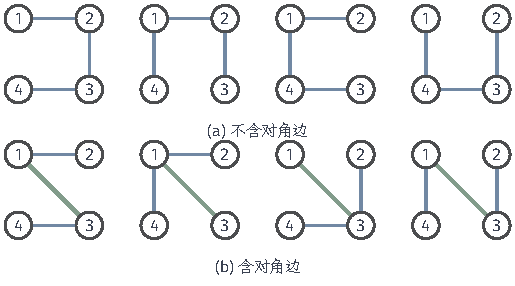
\includegraphics{figures/03-graphs/05-matrices-and-spectra/tikz/sparsification-spanning-trees/figure.pdf}
  \caption{四点五边单位权图的全部$8$棵生成树。上排$4$棵不含对角边$13$，下排$4$棵包含对角边$13$。每条环边（如$12$）在$8$棵树中出现$5$次，故$R_{1,2}=5/8$；对角边$13$在$8$棵树中出现$4$次，故$R_{1,3}=4/8=1/2$。}
  \label{fig:sparsification-spanning-trees}
\end{BookInlineFigure}

由于各边电导均为$1$，生成树包含概率$\mathbb P(e\in T)=c_e R_e$直接等于有效电阻$R_e$。观察图~\ref{fig:sparsification-spanning-trees}：以环边$12$为例，上排$4$棵树中有$3$棵包含它，下排$4$棵树中有$2$棵包含它，共计出现$5$次，故$R_{1,2}=\mathbb P(12\in T)=5/8$；对角边$13$恰好在下排$4$棵树中出现，故$R_{1,3}=\mathbb P(13\in T)=4/8=1/2$。这与第~\ref{sec:electrical-series-parallel}小节通过串并联和拉普拉斯方程算出的结果完全一致。

\subsubsection{Foster定理}
\label{sec:graph-foster-theorem}

对单条边而言，$c_e R_e\in(0,1]$给出了它在随机生成树中的出现概率；如果把全图所有边的$c_e R_e$加起来，总和是多少？由于每一棵生成树都恰好包含$n-1$条边，全图所有边的包含概率之和必定恒等于生成树的边数$n-1$——这就是电网络理论中著名的\term{Foster定理}（Foster's theorem）。

\begin{theorem}[Foster定理]
\label{thm:graph-foster-theorem}
对包含$n$个顶点的连通正权网络$\mathcal G=(V,E,c)$，全体边的电导与有效电阻乘积之和恒等于$n-1$：
\begin{equation}
\sum_{e\in E}c_eR_e=n-1.
\label{eq:graph-foster-sum}
\end{equation}
更一般地，若网络有$k$个正权连通分量，则$\sum_{e\in E}c_e R_e = n-k$。
\end{theorem}

\begin{proof}
我们给出两种相互印证的证明：一种利用随机生成树的期望，另一种利用拉普拉斯伪逆的矩阵迹。

方法一（生成树边数期望法）：在按式~\eqref{eq:graph-weighted-tree-distribution}抽取的随机生成树$T$中，对每条边$e\in E$定义零一指示随机变量$I_e(T)=\mathbb I(e\in T)$。由于任一棵生成树$T$恒有$n-1$条边，必有恒等式$\sum_{e\in E}I_e(T)=n-1$。对等式两边取数学期望，利用期望的线性性及定理~\ref{thm:graph-tree-edge-probability}的$\mathbb E[I_e(T)]=\mathbb P(e\in T)=c_e R_e$，立得
\[
\sum_{e\in E}c_eR_e = \sum_{e\in E}\mathbb P(e\in T) = \mathbb E\!\left[\sum_{e\in E}I_e(T)\right] = n-1.
\]

方法二（拉普拉斯伪逆求迹法）：将$R_e=\bm b_e^\top\bm L^\dagger\bm b_e=\operatorname{tr}(\bm L^\dagger\bm b_e\bm b_e^\top)$代入求和，利用迹的线性性及$\bm L=\sum_{e\in E}c_e\bm b_e\bm b_e^\top$，可得
\[
\sum_{e\in E}c_eR_e
=\operatorname{tr}\!\left(\bm L^\dagger\sum_{e\in E}c_e\bm b_e\bm b_e^\top\right)
=\operatorname{tr}(\bm L^\dagger\bm L).
\]
在连通图上，$\bm L^\dagger\bm L=\bm I-\frac{1}{n}\bm 1\bm 1^\top$是向$n-1$维零和子空间$\bm 1^\perp$上的正交投影矩阵，其迹等于子空间维数$\operatorname{dim}(\bm 1^\perp)=n-1$（当图有$k$个连通分量时，$\bm L$的零空间维数为$k$，投影矩阵的秩与迹均为$n-k$）。
\end{proof}

用四点五边单位权图核对Foster定理：$4$条环边的$c_e R_e$均为$5/8$，对角边的$c_e R_e$为$1/2$，五条边相加得$4\times\frac58+\frac12=3=n-1$。又如在单位权完全图$K_n$中，全部$\binom{n}{2}$条边地位完全对称，由Foster定理无需解方程即可直接读出任意两点间的有效电阻为$R_e=(n-1)/\binom{n}{2}=2/n$。在第~\ref{chap:graph-sparsification}章中，Foster定理给出的归一化常数$\sum_{e\in E}c_e R_e=n-1$将直接把$\{c_e R_e\}_{e\in E}$转化为边抽样概率分布$p_e=\frac{c_e R_e}{n-1}$。

\section{本章小结}
\label{sec:graph-electrical-networks-summary}

给定各顶点的外部注入后，逐边的电流守恒和Ohm定律联立为拉普拉斯方程$\bm L\bm v = \bm b$。正权连通分量内注入总量为零是有解的充要条件。接地选定电势基准——删去的那一列对应已固定的电势，删去的那一行可由其余方程恢复。非连通时各分量独立选基准，孤点注入必须为零。

同一组注入下，电流不唯一决定于守恒条件。不同的守恒流与实际电流之差是环流——它不改变任何顶点的净流出。叠加环流只增加该环流自身的耗散，交叉项因电势与环流正交而消去。实际电流因此是耗散最小的守恒分流，最小耗散同时等于两端压降。这把能量最小原理和有效电阻联系在一起。

计算方式取决于任务。查询单个点对时，解它的单位注入方程再取电势差。树上每条边的电流可以由一侧子树的注入和直接确定，电势由根向叶递推，时间为$O(n)$。若要查询大量点对，可以用一批随机右端给每个顶点预计算低维坐标，之后每次查询只需取两列的平方距离。投影维数和方程求解精度分别控制近似误差和失败概率。

有效电阻在稀疏化与行走中还会出现：第~\ref{chap:graph-sparsification}章用边的有效电阻决定抽样权重，第~\ref{chap:graph-walks}章用点对有效电阻计算随机游走的平均往返时间。


\chapter{图的谱划分}
\label{chap:spectral-partition}

拉普拉斯矩阵零特征值的重数刻画图的连通分量个数。对于连通图，还可以进一步比较跨割边权与割两侧的规模，以识别连接较少的瓶颈并构造划分。

点连通度与边连通度对全图取最小，但不记录分隔后两侧的规模。等周数、导通率和比例割（RatioCut）引入了规模归一化，其一般情形的精确优化是NP难问题。谱方法把离散指示向量放宽为实向量，用特征值给出松弛下界，再沿相应谱坐标扫描候选割。后文将分别说明不同目标的下界、构造算法及其适用的性能保证。

本章记无向图的顶点集为$V$，边集为$E$，顶点数和边数分别为$n=|V|\geq 2$和$m=|E|$，边权非负，连通性按正权支撑判断。第~\ref{sec:graph-algebraic-connectivity}节从连通度的几何意义与不同连通度度量的对比出发，引入代数连通度$\lambda_2$与Fiedler向量$\bm v_2$；第~\ref{sec:graph-cheeger}节建立连接归一化谱$\mu_2$与最小导通率$\phi_*$的Cheeger不等式；第~\ref{sec:graph-ratiocut}至\ref{sec:graph-spectral-partition-comparison}节在此基础上系统展开RatioCut与NCut两种谱划分方法及其对比。

\section{代数连通度}
\label{sec:graph-algebraic-connectivity}

判断一张图是否连通，只需要检查任意两个顶点之间是否存在路径；但要刻画一张连通图“连得有多稳固”，则需要审视它的全局几何形态。本节先通过四类典型图建立“瓶颈”与“稀疏割”的几何图像，再对比局部组合连通度与全局稀疏割度量的局限，由此引出连续可算的代数连通度$\lambda_2$及其对应的Fiedler向量$\bm v_2$。

\subsection{连通度的几何意义}
\label{sec:graph-connectivity-geometry}

连通性只判断任意两点之间是否存在路径。对于已经连通的图，还可以考察删除多少条边会使它断开，以及断开后两侧的规模。图~\ref{fig:graph-connectivity-archetypes}通过四类图比较这些性质。

\begin{BookInlineFigure}
  \centering
  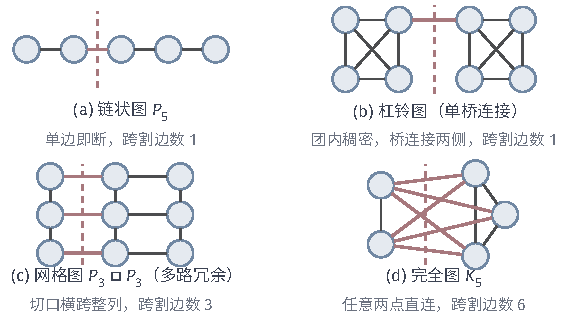
\includegraphics[width=96.238mm]{figures/03-graphs/05-matrices-and-spectra/tikz/connectivity-four-archetypes/figure.pdf}
  \caption{四类典型连通图的瓶颈结构对比。红色虚线标出将图切分为两个较大子集的最薄弱切口，红色实线为被切断的跨割边。(a) 链状图任一内边都是唯一通路；(b) 杠铃图两侧稠密但受制于中间的细腰单桥；(c) 网格图有多条平行通路，切口需横跨整列；(d) 完全图任意两部分之间都有密集边相连。}
  \label{fig:graph-connectivity-archetypes}
\end{BookInlineFigure}

第一类是\emph{链状图}（路径图$P_n$，$n\geq2$）。任意两点之间只有一条路径；删除任意一条边，或在$n\geq3$时删除任意内部顶点，都会使图分为两个连通分量。

第二类是\emph{杠铃图}（barbell graph）。这里取两个完全子图通过一条桥边相连的形式。两个子图内部均有较多连接，但删除中间的桥边就会使两侧断开。因此，局部边数较多并不保证全图没有规模较大的稀疏割。

第三类是\emph{网格图}$P_m\square P_m$（$m\geq2$）。它有$n=m^2$个顶点，每个内部顶点有四个邻居。沿相邻两列之间切开需要删除$m$条边；当$m$为偶数且从中间切开时，两侧顶点数相等。这个例子说明，某些图的均衡切分需要切断随规模增长的多条边。

第四类是\emph{完全图}$K_n$。将顶点集分成大小为$s$和$n-s$的两部分时，割边数为$s(n-s)$。当两侧大小都与$n$同阶时，割边数为$\Theta(n^2)$；若只隔离一个顶点，则只需删除$n-1$条边。讨论切分代价时，需要同时说明两侧的规模。

这些例子提示我们用\emph{稀疏割}（sparse cut）描述图中的连接瓶颈。对非空真子集$S\subsetneq V$，跨割边权为$c(S,\bar S)=\sum_{i\in S,j\in\bar S}w_{i,j}$。只有将它与两侧规模比较，才能区分“隔离一个低度顶点”和“分开两个较大的子图”。后面分别用顶点数与度数总和衡量规模，得到不同的稀疏割指标。

\subsection{连通度的度量}
\label{sec:graph-connectivity-measures}

如何将上述“瓶颈/稀疏割”的几何直觉转化为精确的数学度量？传统图论与组合优化分别从“最弱局部脱节代价”和“全局归一化割代价”两个角度提出了不同的指标，但二者在刻画能力与计算复杂度上各自面临根本困难。

\paragraph{局部组合连通度：$\kappa(\mathcal G)$、$\lambda(\mathcal G)$与$\delta(\mathcal G)$}

在经典图论中，简单无权图$\mathcal G=(V,E)$的连通程度通常由三个离散组合量来度量。第一个量是\term{点连通度}（vertex connectivity）$\kappa(\mathcal G)$，定义为使图变得不连通（或缩为单个顶点）所需删去的最少顶点数。第二个量是\term{边连通度}（edge connectivity）$\lambda(\mathcal G)$，定义为使图变得不连通所需删去的最少边数，即所有非空真子集割的最小割边数：
\begin{equation}
\label{eq:graph-edge-connectivity-def}
  \lambda(\mathcal G) = \min_{\varnothing\neq S\subsetneq V} c(S,\bar S).
\end{equation}
（注意此处带括号的$\lambda(\mathcal G)$表示图$\mathcal G$的边连通度，勿与带下标的拉普拉斯特征值$\lambda_1\leq\lambda_2\leq\cdots\leq\lambda_n$混淆。）第三个量是全图的\term{最小度数}（minimum degree）$\delta(\mathcal G)=\min_{v\in V}d_v$。

对任意顶点$v\in V$，只要删去与$v$关联的全部$d_v$条边，就能将单点$\{v\}$与其余顶点彻底隔开，因此必有$\lambda(\mathcal G)\leq\delta(\mathcal G)$；进一步，从最小边割的每条跨边中适当选取端点删去，又可证明$\kappa(\mathcal G)\leq\lambda(\mathcal G)$（详见定理~\ref{thm:graph-connectivity-comparison}）。三者满足经典的Whitney不等式：
\begin{equation}
\label{eq:graph-whitney-inequality}
  \kappa(\mathcal G) \leq \lambda(\mathcal G) \leq \delta(\mathcal G).
\end{equation}

点连通度$\kappa(\mathcal G)$与边连通度$\lambda(\mathcal G)$都是对全图取最小得到的量，但不记录最小分隔造成的两侧规模。图~\ref{fig:graph-connectivity-local-vs-global}中，$K_5$外接一个叶子与两个$K_4$经单桥相连的图均满足$\kappa=\lambda=1$；前者的最小边割隔离一个顶点，后者则把图分成等大的两部分。这两个指标本身不能区分这两种切分。

\begin{BookInlineFigure}
  \centering
  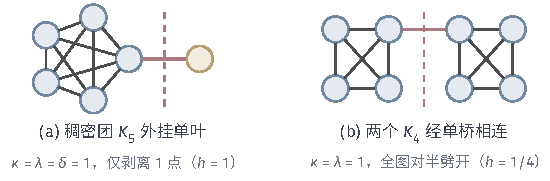
\includegraphics[width=93.059mm]{figures/03-graphs/05-matrices-and-spectra/tikz/connectivity-local-vs-global/figure.pdf}
  \caption{点、边连通度$\kappa(\mathcal G),\lambda(\mathcal G)$与等周数$h(\mathcal G)$的对比。(a) 稠密团$K_5$外挂单个叶子顶点，最弱局部切口仅剥离$1$个末梢顶点；(b) 两个$K_4$经单条桥边相连，最弱切口将全图对半劈开。两张图的$\kappa(\mathcal G)=\lambda(\mathcal G)=1$完全相同，但全局等周数分别为$h=1$与$h=1/4$。}
  \label{fig:graph-connectivity-local-vs-global}
\end{BookInlineFigure}

上述无权连通度只依赖边是否存在，不反映已有边的权重变化。若要比较加权网络，还需要采用割权或谱量。加权最小割值是若干线性函数的最小值，随边权连续变化，但在最优割改变时可能不可微；代数连通度也可能在特征值重合处不可微，因此连续性与可微性应分别讨论。

\paragraph{全局稀疏割指标与NP-Hard计算困境}

为了真正捕捉全局瓶颈，必须在跨割边代价$c(S,\bar S)$的分母上除以两侧子集的规模，迫使指标同时兼顾“割边少”与“两侧大”。按顶点数衡量集合规模时，最自然的全局稀疏割指标是图的\term{等周数}（isoperimetric number，亦称\term{Cheeger常数}）：
\begin{equation}
\label{eq:graph-isoperimetric-number}
  h(\mathcal G) = \min_{\varnothing\neq S\subsetneq V} \frac{c(S,\bar S)}{\min\{|S|,|\bar S|\}},
\end{equation}
以及对称兼顾两侧顶点数的\term{比例割}（RatioCut）：
\begin{equation}
\label{eq:graph-ratiocut-preview}
  \operatorname{RatioCut}(S) = c(S,\bar S)\left(\frac{1}{|S|}+\frac{1}{|\bar S|}\right).
\end{equation}
若改按度数总和（集合体积$\operatorname{vol}(S)=\sum_{i\in S}d_i$）衡量规模，则得到第~\ref{sec:graph-cheeger}节将深入研究的导通率$\phi(S)$与第~\ref{sec:graph-ncut}节的归一化割$\operatorname{NCut}(S)$。

在图~\ref{fig:graph-connectivity-local-vs-global}中，图(a)切下单叶时$\min\{|S|,|\bar S|\}=1$，等周数$h(\mathcal G)=1/1=1$；而图(b)沿桥边对半切开时$\min\{|S|,|\bar S|\}=4$，等周数为$h(\mathcal G)=1/4$，反映了两侧规模不同所带来的指标差异。

然而，这种全局精准性付出了高昂的计算代价：在包含$n$个顶点的图上，非空无序二分共有$2^{n-1}-1$种；精确求解最小等周数$h(\mathcal G)$、最小导通率$\phi_*$或最小RatioCut，均已被证明是\emph{NP-Hard组合优化难题}。当图的顶点数达到数千乃至数百万时，遍历所有离散子集寻找最稀疏割在计算上完全不可行。

因此可以考虑连续松弛：用能够高效近似计算的特征值给出离散割目标的界，再从特征向量构造候选划分。

\subsection{代数连通度}
\label{sec:graph-algebraic-connectivity-variational}

这个连续可算替代品正是组合拉普拉斯矩阵$\bm L=\bm D-\bm W$的第二小特征值$\lambda_2$。为了理解$\lambda_2$为何能度量全局连通程度，我们先从拉普拉斯二次型的沿边能量出发给出它的定义与变分刻画，再证明它与经典连通度及全局稀疏割的定量关系。

\paragraph{代数连通度的定义与变分刻画}

回顾第~\ref{sec:graph-laplacian-energy}节，给每个顶点$i$赋予实数值$x_i$时，组合拉普拉斯二次型
\[
  \bm x^\top\bm L\bm x = \sum_{\{i,j\}\in E} w_{i,j}(x_i-x_j)^2
\]
累加了所有边两端读数差的平方，衡量向量$\bm x$在图上的沿边变化能量。例如在图~\ref{fig:graph-partition-edge-energy}(a)的单位权四点路径上，给前两个顶点赋$+1$、后两个赋$-1$，只有中间边$23$产生差值$1-(-1)=2$，总能量为$4$；而在图~\ref{fig:graph-partition-edge-energy}(b)中添入跨接首尾的边$14$后，同一赋值的总能量增至$8$。

\begin{BookInlineFigure}
  \centering
  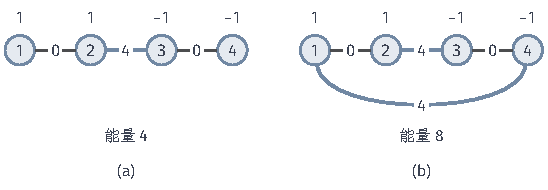
\includegraphics{figures/03-graphs/05-matrices-and-spectra/tikz/partition-edge-energy/figure.pdf}
  \caption{对同一组顶点赋值计算沿边能量。(a) 四点路径，只有中间边贡献了能量$4$。(b) 加上边$14$后得到四边环，新增的边上也有差$2$，总能量变为$8$。顶点上方是赋值，边上的数是差的平方。}
  \label{fig:graph-partition-edge-energy}
\end{BookInlineFigure}

要在给定图上寻找“沿边能量最小”的非平凡顶点赋值，必须满足两条规范化约束。第一，给所有顶点赋相同的常数时，每条边两端差均为零，能量恒为零；这种常值赋值不反映任何图结构信息，因此需要要求赋值向量与全一常向量正交，即满足零和条件$\bm x\perp\bm 1$（$\sum_{i=1}^n x_i=0$）。

第二，将非零向量$\bm x$同乘常数$c\neq 0$会使能量$\bm x^\top\bm L\bm x$与欧氏长度平方$\bm x^\top\bm x$同步放大$c^2$倍；为了在同一尺度下公平比较不同方向，应当考察两者的比值——即Rayleigh商$\frac{\bm x^\top\bm L\bm x}{\bm x^\top\bm x}$。Fiedler于1973年提出将非平凡方向上的最小Rayleigh商定义为图的代数连通度。

\begin{definition}[代数连通度]
\label{def:graph-algebraic-connectivity}
设$n$阶无向非负加权图$\mathcal G$的组合拉普拉斯矩阵$\bm L$的特征值按升序排列为$0=\lambda_1\leq\lambda_2\leq\cdots\leq\lambda_n$。图的\term{代数连通度}（algebraic connectivity）定义为第二小特征值$\lambda_2(\mathcal G)$（在不致混淆时简记为$\lambda_2$），其Courant--Fischer变分刻画为
\begin{equation}
\label{eq:graph-algebraic-connectivity}
\lambda_2
=\min_{\substack{\bm x\perp\bm 1\\\bm x\ne\bm 0}}
\frac{\bm x^\top\bm L\bm x}{\bm x^\top\bm x}
=\min_{\substack{\bm x^\top\bm 1=0\\\lVert\bm x\rVert_2=1}}
\bm x^\top\bm L\bm x.
\end{equation}
\end{definition}

将式~\eqref{eq:graph-algebraic-connectivity}与前文的正交特征展开相对照，可以一步看清该极小值的代数结构。设$\bm v_1=\bm 1/\sqrt{n},\bm v_2,\ldots,\bm v_n$为$\bm L$对应于$0=\lambda_1\leq\lambda_2\leq\cdots\leq\lambda_n$的标准正交特征向量基。

任取满足$\bm x\perp\bm 1$的非零向量$\bm x$，它在$\bm v_1$方向上的投影系数为零，故可展开为$\bm x=\sum_{k=2}^n\alpha_k\bm v_k$。

代入Rayleigh商并利用特征向量的正交性，可得
\[
  \frac{\bm x^\top\bm L\bm x}{\bm x^\top\bm x}
  = \frac{\sum_{k=2}^n\lambda_k\alpha_k^2}{\sum_{k=2}^n\alpha_k^2}
  \geq \lambda_2,
\]
且当$\bm x$取为$\lambda_2$对应的特征向量$\bm v_2$时等号精确成立。

由这一变分刻画立即可读出代数连通度的三项基本性质：
\begin{enumerate}
\item \emph{连通性的充要判据}：由第~\ref{sec:graph-laplacian-kernel}小节知，$\bm L$的零特征值重数等于图$\mathcal G$的连通分量个数。因此$\lambda_2>0$当且仅当$\mathcal G$连通；$\lambda_2=0$当且仅当$\mathcal G$不连通。
\item \emph{关于边权与加边的单调性}：若在相同顶点集上增大边权或添加新边得到$\mathcal G'$，则对每个零和向量$\bm x$都有$\bm x^\top\bm L(\mathcal G')\bm x\geq\bm x^\top\bm L(\mathcal G)\bm x$，取最小后即得$\lambda_2(\mathcal G')\geq\lambda_2(\mathcal G)$。
\item \emph{典型图族的定量对比}：结合第~\ref{sec:graph-typical-laplacian-spectra}小节算出的典型图谱，四类典型图（图~\ref{fig:graph-connectivity-archetypes}）的代数连通度呈现出鲜明的量级差异：链状路径图$\lambda_2(P_n)=2\bigl(1-\cos(\pi/n)\bigr)=\Theta(n^{-2})$，随$n$增大迅速衰减至$0$；由两个$K_m$经单桥相连的杠铃图（$m\geq2$，$n=2m$）满足$\lambda_2=\bigl(m+2-\sqrt{(m+2)^2-8}\bigr)/2=\Theta(m^{-1})=\Theta(n^{-1})$，定量暴露出细腰瓶颈；二维网格图$\lambda_2(P_m\square P_m)=2\bigl(1-\cos(\pi/m)\bigr)=\Theta(n^{-1})$，比链状图高出一个量级；而完全图$\lambda_2(K_n)=n$随规模线性增长，成为所有$n$阶简单无权图的上界。
\end{enumerate}

\paragraph{代数连通度与其他连通度的关系}

代数连通度$\lambda_2$不仅在定性趋势上区分了不同图族，而且与前文介绍的局部组合连通度$\kappa(\mathcal G),\lambda(\mathcal G),\delta(\mathcal G)$以及全局稀疏割指标$h(\mathcal G),\operatorname{RatioCut}$之间存在严格的不等式联系。我们先证明Fiedler关于局部连通度的经典上界定理。

\begin{theorem}[代数连通度与点、边连通度的比较]
\label{thm:graph-connectivity-comparison}
设$\mathcal G=(V,E)$为有限简单无权连通非完全图，则其代数连通度$\lambda_2(\mathcal G)$、点连通度$\kappa(\mathcal G)$、边连通度$\lambda(\mathcal G)$与最小度数$\delta(\mathcal G)$满足
\begin{equation}
\label{eq:graph-connectivity-comparison}
  \lambda_2(\mathcal G)\leq\kappa(\mathcal G)\leq\lambda(\mathcal G)\leq\delta(\mathcal G).
\end{equation}
\end{theorem}

\begin{proof}
我们按从左到右的顺序分三步证明式~\eqref{eq:graph-connectivity-comparison}中的三个不等号。

第一步：证明$\lambda_2(\mathcal G)\leq\kappa(\mathcal G)$。因为$\mathcal G$是连通非完全图，必存在最小点分隔集$T\subsetneq V$（$|T|=\kappa(\mathcal G)$），使得删去$T$后剩余顶点集$V\setminus T$至少分裂为两个互不相连的非空部分。取其中一个连通块记为$A$，将其余所有块合并记为$B=V\setminus(T\cup A)$，则$A,B$均非空，且$A$与$B$之间没有任何直接边相连。

构造如下三值试探向量$\bm x\in\mathbb R^n$：对$i\in A$令$x_i=|B|$，对$i\in B$令$x_i=-|A|$，对$i\in T$令$x_i=0$。

核对零和条件：$\bm x$的各分量之和为
\[
  \sum_{i=1}^n x_i = |A|\cdot|B| + |B|\cdot(-|A|) + |T|\cdot 0 = 0,
\]
故$\bm x\perp\bm 1$且$\bm x\neq\bm 0$。

计算分母的欧氏长度平方：
\[
  \bm x^\top\bm x = |A|\cdot|B|^2 + |B|\cdot|A|^2 = |A||B|(|A|+|B|).
\]

计算分子的沿边能量$\bm x^\top\bm L\bm x$：$A$内部各点取值恒为$|B|$，差为零；$B$内部各点取值恒为$-|A|$，差为零；$T$内部各点取值恒为$0$，差也为零；而$A$与$B$之间无边。因此，只有一端在$T$、另一端在$A$或$B$的边才对能量有贡献。

由于$\mathcal G$是简单无权图，$A$中的每个顶点至多与$T$中的$|T|$个顶点相邻，每条这样的边贡献$(|B|-0)^2=|B|^2$；同理，$B$中的每个顶点至多与$T$中的$|T|$个顶点相邻，每条这样的边贡献$(-|A|-0)^2=|A|^2$。累加可得分子上界：
\[
  \bm x^\top\bm L\bm x
  \leq |T|\bigl(|A|\cdot|B|^2 + |B|\cdot|A|^2\bigr)
  = |T|\cdot|A||B|(|A|+|B|).
\]

将分子上界除以分母$\bm x^\top\bm x$，结合变分刻画式~\eqref{eq:graph-algebraic-connectivity}即得
\[
  \lambda_2(\mathcal G)\leq\frac{\bm x^\top\bm L\bm x}{\bm x^\top\bm x}\leq |T|=\kappa(\mathcal G).
\]

第二步：证明$\kappa(\mathcal G)\leq\lambda(\mathcal G)$。取一个大小为$\lambda(\mathcal G)$的最小边割$c(S,\bar S)$。若在两侧能找到一对不相邻的顶点$u\in S$与$v\in\bar S$，则每条跨割边至少有一个端点不属于$\{u,v\}$；从每条跨割边各选一个异于$u,v$的端点组成集合$T$，则$|T|\leq\lambda(\mathcal G)$且删去$T$即切断了$u$与$v$之间的所有跨边，故$\kappa(\mathcal G)\leq|T|\leq\lambda(\mathcal G)$。

若$S$与$\bar S$之间的所有可能边都存在，设$|S|=p,|\bar S|=q$，则$\lambda(\mathcal G)=pq$；由$(p-1)(q-1)\geq 0$知$pq\geq p+q-1=n-1$，而在非完全图中任取一对不相邻顶点并删去其余$n-2$个顶点即可断开图，故仍有$\kappa(\mathcal G)\leq n-2<n-1\leq\lambda(\mathcal G)$。

第三步：证明$\lambda(\mathcal G)\leq\delta(\mathcal G)$。取达到最小度数的顶点$v_0$（$d_{v_0}=\delta(\mathcal G)$），令$S=\{v_0\}$，则割$(S,\bar S)$恰好切断与$v_0$关联的$\delta(\mathcal G)$条边，故$\lambda(\mathcal G)\leq c(\{v_0\},V\setminus\{v_0\})=\delta(\mathcal G)$。
\end{proof}

在单位权四点路径$P_4$上，$\lambda_2=2-\sqrt 2\approx 0.586<\kappa(P_4)=\lambda(P_4)=\delta(P_4)=1$；在四元环$C_4$上，$\lambda_2=\kappa(C_4)=\lambda(C_4)=\delta(C_4)=2$，不等式链全部取等（图~\ref{fig:graph-connectivity-separator-trial}）。完全图$K_n$之所以在定理~\ref{thm:graph-connectivity-comparison}中单独排除，是因为$K_n$中不存在不相邻的顶点对，无法删点将其分成两个不相连的非空部分，按约定$\kappa(K_n)=\lambda(K_n)=\delta(K_n)=n-1$，而$\lambda_2(K_n)=n$。

\begin{BookInlineFigure}
  \centering
  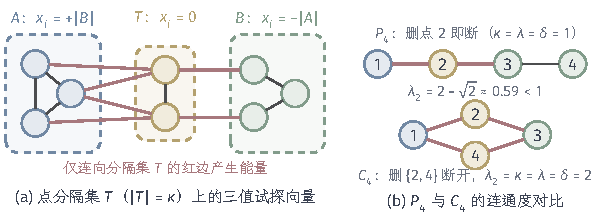
\includegraphics[width=102.164mm]{figures/03-graphs/05-matrices-and-spectra/tikz/connectivity-separator-trial/figure.pdf}
  \caption{点分隔集试探向量构造与连通度不等式核对。(a) 删去最小点分隔集$T$（$|T|=\kappa$）将图分为互不相连的$A$与$B$；给$A$赋$+|B|$、$B$赋$-|A|$、$T$赋$0$后，仅连向$T$的红边产生沿边能量。(b) $P_4$（严格不等式）与$C_4$（等号成立）的连通度对比。}
  \label{fig:graph-connectivity-separator-trial}
\end{BookInlineFigure}

除了受局部连通度$\kappa(\mathcal G)$上界控制之外，代数连通度$\lambda_2$还直接给出了全局等周数$h(\mathcal G)$与最小RatioCut的\emph{连续下界}。对任意非空真子集$S\subsetneq V$（记$s=|S|,t=|\bar S|=n-s$），在式~\eqref{eq:graph-algebraic-connectivity}中代入中心化两值试探向量$\bm y=\bm 1_S-\frac{s}{n}\bm 1$（详见第~\ref{sec:graph-ratiocut-relaxation}小节定理~\ref{prop:graph-ratiocut-relaxation}），立即可得
\begin{equation}
\label{eq:algebraic-connectivity-isoperimetric-bound}
  \lambda_2(\mathcal G)
  \leq \frac{\bm y^\top\bm L\bm y}{\bm y^\top\bm y}
  = c(S,\bar S)\left(\frac{1}{|S|}+\frac{1}{|\bar S|}\right)
  = \operatorname{RatioCut}(S)
  \leq \frac{2\,c(S,\bar S)}{\min\{|S|,|\bar S|\}}.
\end{equation}
对所有非空真子集$S$取最小后，即得全局稀疏割的下界关系：
\begin{equation}
\label{eq:algebraic-connectivity-cheeger-lower}
  \frac{\lambda_2(\mathcal G)}{2}
  \leq \frac{1}{2}\min_{\varnothing\neq S\subsetneq V}\operatorname{RatioCut}(S)
  \leq h(\mathcal G).
\end{equation}
式~\eqref{eq:algebraic-connectivity-cheeger-lower}给出了按顶点数归一化的割权下界：$h(\mathcal G)\geq\lambda_2/2$。这里的尺度仍依赖边权；把全部边权同乘常数会使$\lambda_2$和$h$同比变化。若希望指标对这种整体缩放不变，可以改用度加权体积作分母，这将引出下一节的导通率与归一化拉普拉斯。

\subsection{Fiedler向量}
\label{sec:graph-fiedler-vector}

代数连通度$\lambda_2$给出割权的谱下界，而相应的特征向量$\bm v_2$提供一维顶点坐标，可据此构造候选划分。它一般不直接给出最优稀疏割。

\begin{definition}[Fiedler向量]
\label{def:graph-fiedler-vector}
设连通无向非负加权图$\mathcal G$的组合拉普拉斯矩阵为$\bm L$。对应于代数连通度$\lambda_2>0$的非零特征向量$\bm v_2$（即满足$\bm L\bm v_2=\lambda_2\bm v_2$且$\bm v_2^\top\bm 1=0$，亦常记作$\bm f$）称为图的\term{Fiedler向量}（Fiedler vector）。
\end{definition}

如果$\lambda_2$是单重特征值，单位长度的Fiedler向量在差一个正负号的意义下唯一确定；若$\lambda_2$为重根，则对应的特征子空间中任意非零向量都是Fiedler向量。由于连通图上$\bm v_2\perp\bm 1$，Fiedler向量的所有分量之和为零：$\sum_{i=1}^n(\bm v_2)_i=0$，因此它必然同时包含正分量与负分量。

\paragraph{Fiedler向量$\bm v_2$的物理与几何意义}

我们可以从弹簧势能、振动和扩散三个角度理解$\bm v_2$为何可用于构造划分。

第一个视角是\emph{一维胡克弹簧网络的最小势能嵌入}。将图中的每条边$\{i,j\}$看作劲度系数为$w_{i,j}$的理想弹簧，把每个顶点$i$放置在实数轴上的坐标$x_i=(\bm v_2)_i$处，则拉普拉斯二次型的一半$\frac12\bm x^\top\bm L\bm x=\frac12\sum_{\{i,j\}\in E}w_{i,j}(x_i-x_j)^2$恰好是整个弹簧系统的总弹性势能。零和条件$\sum_i x_i=0$将全部顶点的重心固定在原点$0$，单位长度条件$\sum_i x_i^2=1$则固定了顶点在实轴上的总展开尺度，防止所有顶点坍缩到原点以逃避势能。

在零和与单位长度约束下，最小化Rayleigh商等价于最小化上述弹簧势能。图~\ref{fig:graph-fiedler-barbell}中的两个三角形仅由边$3\!-\!4$连接，其Fiedler向量在两个三角形上分别取负值和正值，团内坐标差小于桥边两端的坐标差。这说明该图的低能量方向能够反映桥边所连接的两个部分；对于一般图，仍须计算各候选割的目标值来判断划分质量。

\begin{BookInlineFigure}
  \centering
  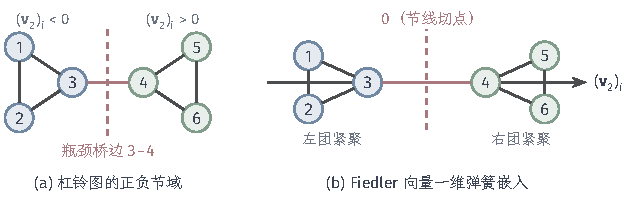
\includegraphics[width=107.495mm]{figures/03-graphs/05-matrices-and-spectra/tikz/fiedler-barbell-embedding/figure.pdf}
  \caption{杠铃图上Fiedler向量$\bm v_2$的物理意义与一维弹簧嵌入。(a) 两个三角形团$\{1,2,3\}$与$\{4,5,6\}$经单条瓶颈桥边$3\!-\!4$相连，$\bm v_2$在左团取负值、右团取正值；(b) 将顶点放置在实轴坐标$(\bm v_2)_i$上时，团内密集弹簧将各自顶点紧紧聚拢在两侧，唯一的瓶颈桥边被大幅拉伸并跨越原点$0$（红色虚线切点）。}
  \label{fig:graph-fiedler-barbell}
\end{BookInlineFigure}

第二个视角是\emph{弹性振动的基频驻波模态}。在质量均匀的离散振动网络$\frac{\mathrm d^2\bm u}{\mathrm dt^2}=-\bm L\bm u$中，$\lambda_1=0$对应全体顶点同向平移的刚体运动（零频模态），而$\lambda_2>0$对应的$\bm v_2$则是系统的第一阶非平凡简谐振动模态（基频驻波）。正负分量表示相反的振动相位，角频率为$\sqrt{\lambda_2}$。在上述杠铃图中，两团以相反相位振动；一般图的符号边界不保证对应最优稀疏割。

第三个视角是\emph{图上热扩散的最慢衰减模态}。在连续时间热传导或共识扩散方程$\frac{\mathrm d\bm x}{\mathrm dt}=-\bm L\bm x$中，任意初始温度分布$\bm x(0)=\sum_{k=1}^n\alpha_k\bm v_k$按$\bm x(t)=\alpha_1\bm v_1+\sum_{k=2}^n\alpha_k\mathrm e^{-\lambda_k t}\bm v_k$演化。非恒定模态按各自的$\mathrm e^{-\lambda_k t}$衰减，最小正特征值$\lambda_2$对应最慢衰减率。若$\lambda_2$为重特征值，整个对应特征子空间具有相同的衰减率；该部分是否出现在演化中，还取决于初值在此子空间上的投影。

\paragraph{Fiedler节域连通性定理}

按Fiedler向量的符号可以构造二分候选。下面的Fiedler节域连通性定理保证非负顶点集和非正顶点集各自诱导连通子图；这是一项连通性结论，不是割目标最优性的保证。

\begin{theorem}[Fiedler节域连通性定理]
\label{thm:graph-fiedler-connected-side}
设有限无向加权图$\mathcal G$的正权支撑连通，$\bm f=\bm v_2$为组合拉普拉斯矩阵$\bm L$的Fiedler向量。则非负顶点集合$V_+=\{i\in V:f_i\geq 0\}$（以及对称地，非正顶点集合$V_-=\{i\in V:f_i\leq 0\}$）所诱导的正权子图必定连通。
\end{theorem}

\begin{proof}
由$\bm f$与$-\bm f$的对称性，只需证明$V_+=\{i:f_i\geq 0\}$诱导的正权子图连通。反设$V_+$分裂成了两个或更多个互不连通的连通块，我们将导出矛盾。

第一步：写出单个非负连通块上的特征方程。记严格负值顶点集合为$N=\{j\in V:f_j<0\}$，任取$V_+$的一个连通块$C$。由于$V_+$的不同连通块之间没有正权边相连，特征方程$\bm L\bm f=\lambda_2\bm f$限制在块$C$的坐标上只涉及$C$自身与负值集$N$：
\[
  \bm L_{C,C}\bm f_C = \lambda_2\bm f_C - \bm r_C,
  \qquad
  \bm r_C = \bm L_{C,N}\bm f_N.
\]
矩阵块$\bm L_{C,N}$的元素为$-w_{i,j}\leq 0$（$i\in C,j\in N$），而$\bm f_N$的分量全部严格为负，故$\bm r_C$的每个分量$(\bm r_C)_i=\sum_{j\in N}w_{i,j}(-f_j)\geq 0$。又因原图连通且$C$不与$V_+\setminus C$相连，$C$至少有一条正权边连向$N$，从而$\bm r_C$是逐项非负且至少有一项严格为正的向量。

第二步：利用块主子矩阵的正Perron向量证明$\theta_C<\lambda_2$。取实数$a>0$足够大，使$\bm M_C=a\bm I-\bm L_{C,C}$逐项非负。因为$C$诱导的正权子图连通，沿用第~\ref{sec:adjacency-perron-theorem}节Perron定理的证明（对角非负项不影响取绝对值和沿正权边传播的论证，单点块可直接验证），$\bm M_C$的最大特征值对应的特征向量可取为分量全部严格为正的向量$\bm z>\bm 0$。若记$\theta_C$为对称块$\bm L_{C,C}$的最小特征值，则$a-\theta_C$正是$\bm M_C$的最大特征值，故$\bm L_{C,C}\bm z=\theta_C\bm z$。

将第一步的块方程左乘$\bm z^\top$，利用$\bm z^\top\bm L_{C,C}=\theta_C\bm z^\top$可得
\[
  \theta_C\,\bm z^\top\bm f_C
  = \lambda_2\,\bm z^\top\bm f_C - \bm z^\top\bm r_C.
\]
注意$\bm f_C\geq\bm 0$且不可能全为零（若$\bm f_C=\bm 0$，则由第一步方程得$\bm r_C=\bm 0$，与$\bm r_C$至少有一项为正矛盾）。结合$\bm z>\bm 0$可知$\bm z^\top\bm f_C>0$且$\bm z^\top\bm r_C>0$。两边同除以$\bm z^\top\bm f_C$即得
\[
  \theta_C = \lambda_2 - \frac{\bm z^\top\bm r_C}{\bm z^\top\bm f_C} < \lambda_2.
\]
这表明$V_+$的每一个连通块$C$的最小特征值$\theta_C$都严格小于$\lambda_2$。

第三步：由Cauchy交错定理导出矛盾。若$V_+$至少有两个连通块$C_1,C_2$，则$\bm L$在$V_+$上的主子矩阵$\bm L_{V_+,V_+}$是以各连通块$\bm L_{C_r,C_r}$为对角块的分块对角矩阵，其全体特征值是各块特征值的并集。由于$\theta_{C_1}<\lambda_2$且$\theta_{C_2}<\lambda_2$，主子矩阵$\bm L_{V_+,V_+}$至少有两个特征值严格小于$\lambda_2$，即其第二小特征值$\lambda_2(\bm L_{V_+,V_+})<\lambda_2(\bm L)$。但这直接违背了实对称矩阵主子矩阵的Cauchy交错定理（见\BookChapterRef{chap:eigen-spectral-decomposition}{卷二“谱分解”章}：任意主子矩阵的第$k$小特征值不低于原矩阵的第$k$小特征值）。矛盾说明$V_+$只能包含唯一一个连通块。
\end{proof}

需要注意，定理~\ref{thm:graph-fiedler-connected-side}包含零坐标顶点（$f_i\geq 0$）。如图~\ref{fig:graph-fiedler-star-zero}所示，在有四片叶子的五顶点星图$K_{1,4}$上，中心顶点度为$4$，四片叶子度均为$1$；取中心分量为$0$、四片叶子分量依次为$+1,+1,+1,-3$，容易验证它是对应于$\lambda_2=1$的Fiedler向量。此时非负集合$V_+$由中心和三片取$+1$的叶子组成，通过中心保持连通；但如果只取严格正值集合$\{i:f_i>0\}$，三片叶子之间互不相连，不再连通。

\begin{BookInlineFigure}
  \centering
  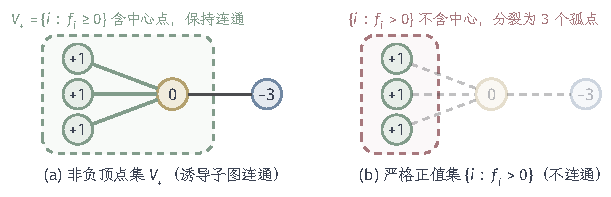
\includegraphics[width=103.396mm]{figures/03-graphs/05-matrices-and-spectra/tikz/fiedler-star-zero-center/figure.pdf}
  \caption{五顶点星图$K_{1,4}$上Fiedler向量$\bm f=(1,1,1,0,-3)^\top$的节域结构。(a) 非负集合$V_+=\{i:f_i\geq 0\}$包含取值为$0$的中心顶点，诱导子图保持连通；(b) 严格正值集合$\{i:f_i>0\}$不含中心顶点，分裂为三个孤立叶子。}
  \label{fig:graph-fiedler-star-zero}
\end{BookInlineFigure}

Fiedler向量$\bm v_2$通过一维连续坐标为所有顶点排出了反映瓶颈结构的自然顺序。在此基础上，接下来两节将进一步解决两个关键问题：第~\ref{sec:graph-cheeger}节引入归一化拉普拉斯与Cheeger不等式，严格证明沿谱方向扫描阈值必定能找到逼近全局最优导通率的稀疏割；第~\ref{sec:graph-ratiocut}至\ref{sec:graph-spectral-partition-comparison}节则给出RatioCut与NCut的完整谱划分算法。

\section{Cheeger不等式}
\label{sec:graph-cheeger}

前一节用组合拉普拉斯的第二小特征值$\lambda_2$衡量图连得有多紧。但$\lambda_2$会随边权的整体放大而增大，两张规模不同的图之间直接比较$\lambda_2$并不公平。

一种更合理的衡量方式是：割掉一组边后，组间断开的边权占较小一侧总连接量的多少？如果一座大桥连接两个城市群，桥虽然只有一条，但两侧各自有大量内部道路，切断这一条边对较小一侧的影响取决于那一侧总共有多少路。相比之下，切下一个只有一条边的孤立叶子，割权同为一，但那个叶子的全部连接就是这一条边。

以下假定正权支撑连通，这保证每个顶点都有正度。

\subsection{导通率}
\label{sec:graph-conductance}

用$S$和$\bar S=V\setminus S$表示一组顶点和剩下的顶点，要求两组都非空。把一端在$S$、另一端在$\bar S$的边各数一次，将它们的权重相加，得到\term{割权}（cut weight）$c(S,\bar S)$。

顶点$i$的加权度$d_i$是连到该点的所有边权之和。将$S$内每个点的度累加，得到集合体积$\operatorname{vol}(S)=\sum_{i\in S}d_i$。体积的计算中，组内边在两个端点各被计入一次，跨边只在组内的那个端点计入。图~\ref{fig:graph-conductance-volume}标出了这两种计数。

\begin{BookInlineFigure}
  \centering
  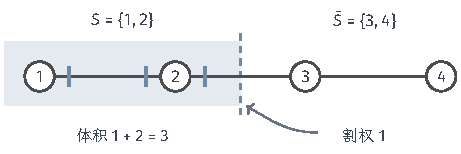
\includegraphics{figures/03-graphs/05-matrices-and-spectra/tikz/conductance-volume/figure.pdf}
  \caption{单位权四点路径上$S=\{1,2\}$的体积计算。每道刻度表示一个边端点处计入的一份。边$12$两端都在$S$中，计两份；边$23$只有一端在$S$中，计一份。左侧体积为$3$。虚线切过的边只有$23$，割权为$1$。}
  \label{fig:graph-conductance-volume}
\end{BookInlineFigure}

用体积较小的一侧来衡量规模。分母越小，同样的割权所占的比例就越大。

\begin{definition}[导通率]
\label{def:graph-conductance}
集合的\term{导通率}（conductance）和图的最小导通率分别为
\begin{equation}
\label{eq:graph-conductance}
\phi(S)=\frac{c(S,\bar S)}
  {\min\{\operatorname{vol}(S),\operatorname{vol}(\bar S)\}},
\qquad
\phi_*=\min_{\varnothing\ne S\subsetneq V}\phi(S).
\end{equation}
\end{definition}

在单位权四点路径上试两种切法。把中间边$23$切断，得到$\{1,2\}$和$\{3,4\}$。顶点$1$的度为$1$，顶点$2$的度为$2$，左侧体积为$1+2=3$。右侧的度分别为$2,1$，体积也为$3$。跨边只有一条，割权为$1$，所以这个割的导通率为$1/3$。

如果只切下端点$1$，割权仍为$1$，但$\{1\}$的体积只有$1$，另一侧体积为$5$。导通率变成$1/1=1$。

两种割的割权相同，但中间割的较小一侧承载了更多连接（体积$3$对$1$），所以按比例算，中间割更"高效"。在所有切法中选最小的导通率，就是图的$\phi_*$。

接下来要用归一化拉普拉斯的第二小特征值$\mu_2$来控制$\phi_*$。回顾第~\ref{sec:graph-normalized-laplacian}节，对称归一化拉普拉斯$\mathcal L=\bm D^{-1/2}\bm L\bm D^{-1/2}$的变分刻画为
\begin{equation}
\label{eq:graph-normalized-variational-cut}
\mu_2=\min_{\substack{\bm f^\top\bm D\bm1=0\\\bm f\ne\bm0}}
       \frac{\bm f^\top\bm L\bm f}{\bm f^\top\bm D\bm f}.
\end{equation}
这里的分母把每个坐标的平方乘以该点的度再求和，而不是简单的平方和。零方向对应的条件也变成度加权的零和$\sum_i d_i f_i=0$。若将$S$内的坐标设为$1$，其余设为$0$，分母恰好是$\operatorname{vol}(S)$。因此体积与归一化谱之间有了直接联系。

\begin{theorem}[\term{Cheeger不等式}]
\label{thm:graph-cheeger}
有限无向非负权图的正权支撑连通，且至少有两个顶点时，
\begin{equation}
\label{eq:graph-cheeger}
\frac{\mu_2}{2}\leq\phi_*\leq \sqrt{2\mu_2}.
\end{equation}
\end{theorem}

两个界各回答一个问题。下界说：无论怎样选择分组，其导通率都至少为$\mu_2/2$，图中不存在比这更稀疏的平衡割。上界则提供了一种构造性的搜索：按第二特征方向的分量给顶点排序，依次尝试切点，其中至少有一个割的导通率不超过$\sqrt{2\mu_2}$。

下面分别证明这两个界。

\subsection{下界：指示向量的Rayleigh商}
\label{sec:graph-cheeger-lower}

为证明下界，我们从任意一个割出发，构造一个满足约束的试探向量，再把它代入式~\eqref{eq:graph-normalized-variational-cut}。

取任意非空真子集$S$，设$a=\operatorname{vol}(S)\leq\operatorname{vol}(\bar S)=b$。从$S$的指示向量$\bm 1_S$出发，把每个坐标减去度加权平均值$a/(a+b)$，得到
\[
\bm f=\bm1_S-\frac{a}{a+b}\bm1.
\]
$\bm f$在$S$上取值$b/(a+b)$，在$\bar S$上取值$-a/(a+b)$。度加权的坐标和为
\[
a\cdot\frac{b}{a+b}+b\cdot\frac{-a}{a+b}=0,
\]
满足零和条件$\bm f^\top\bm D\bm 1=0$。

下面分别计算分子和分母。对组内的一条边，两端取同一个值，差为零，不贡献能量。对跨边，两端分别取$b/(a+b)$和$-a/(a+b)$，差恰好为$1$。因此分子等于割权：
\[
\bm f^\top\bm L\bm f=c(S,\bar S).
\]

分母将两侧的常数平方各按体积累加：
\[
\bm f^\top\bm D\bm f
=a\left(\frac{b}{a+b}\right)^{\!2}
+b\left(\frac{a}{a+b}\right)^{\!2}
=\frac{ab}{a+b}.
\]

$\mu_2$是所有合格向量中Rayleigh商的最小值。把$\bm f$代入，给出上界
\[
\mu_2
\leq\frac{c(S,\bar S)}{\dfrac{ab}{a+b}}
=c(S,\bar S)\left(\frac{1}{a}+\frac{1}{b}\right).
\]
因为$a\leq b$，有$1/b\leq 1/a$，所以
\[
\frac{1}{a}+\frac{1}{b}\leq\frac{2}{a}
=\frac{2}{\min\{\operatorname{vol}(S),\operatorname{vol}(\bar S)\}}.
\]
代入得$\mu_2\leq 2\phi(S)$。这个结论对每个非空真子集$S$都成立，因此对所有割取最小后，$\mu_2/2\leq\phi_*$。

用四点路径的中间割核对。两侧体积$a=b=3$，中心化后两侧的坐标分别为$1/2$和$-1/2$。只有一条跨边，割权为$1$。分母为$3\cdot(1/2)^2+3\cdot(1/2)^2=3/2$。代入得$\mu_2\leq 1/(3/2)=2/3$，恰好是$2\phi(S)=2\cdot(1/3)$。

\subsection{上界：扫描阈值}
\label{sec:graph-cheeger-sweep}

下界告诉我们导通率不可能太小。上界则要找到一个具体的割来展示它也不会太大。思路是从归一化拉普拉斯的第二特征方向出发，对顶点排序后逐个阈值切开，证明其中至少有一个割的导通率不超过$\sqrt{2\mu_2}$。

证明分三步。第一步从特征方向中选出一侧体积不超过半图的非负向量。第二步用积分论证，说明沿该向量的阈值扫描中，导通率的加权平均可以用能量商控制。第三步用Cauchy--Schwarz不等式把能量商和$\mu_2$联系起来。

\paragraph{第一步：选出合适的一侧}

设$\bm f$是式~\eqref{eq:graph-normalized-variational-cut}的一个最优向量，能量商恰为$\mu_2$。按分量从小到大排列各顶点，逐个累计加权度。累计首次达到$\operatorname{vol}(V)/2$时，取该顶点的分量值作为度加权中位数$\tau$。严格小于$\tau$的顶点体积不超过半图，严格大于$\tau$的也不超过半图。

将$\bm f$平移为$\bm h=\bm f-\tau\bm 1$。平移对每条边的差没有影响，所以能量$\bm h^\top\bm L\bm h=\bm f^\top\bm L\bm f$不变。对于度加权平方和，展开得到
\[
\bm h^\top\bm D\bm h
=\bm f^\top\bm D\bm f
-2\tau\underbrace{\bm f^\top\bm D\bm 1}_{=\,0}
+\tau^2\operatorname{vol}(V)
=\bm f^\top\bm D\bm f+\tau^2\operatorname{vol}(V).
\]
分子不变，分母没有减小，因此$\bm h$的能量商不超过$\mu_2$。

把$\bm h$分成正部$\bm g^+$和负部$\bm g^-$两个非负向量：$g^+_i=\max(h_i,0)$，$g^-_i=\max(-h_i,0)$。它们的度加权平方和相加恰等于$\bm h$的度加权平方和。

逐边比较能量。若两端同号（均正或均负），差完全保留在同一部分中。若一端为$p>0$、另一端为$-q<0$，原来的差平方为$(p+q)^2$，而拆开后正部贡献$p^2$，负部贡献$q^2$，合计$p^2+q^2\leq(p+q)^2$。因此两部分的能量之和不超过原来的能量。

如果两个非零部分的能量商都严格大于$\mu_2$，把它们的能量分别用$\mu_2$乘平方和的下界代入，加起来就会超过$\mu_2$乘原平方和，而左侧能量之和又不超过原能量——矛盾。所以至少有一个非零部分$\bm g$的能量商不超过$\mu_2$。这个$\bm g$非负，且它的非零支撑的体积至多为$\operatorname{vol}(V)/2$。

\paragraph{第二步：积分论证}

对$t\geq0$，定义集合$S_t=\{i:g_i^2>t\}$。随着$t$增大，$S_t$逐渐缩小。$t$的连续变化只在经过某个$g_i^2$时才改变集合，因此实际上只需处理有限个阈值。

先计算体积对阈值的积分。顶点$i$当且仅当$0\leq t<g_i^2$时被$S_t$选入，此时它对体积的贡献为$d_i$。把所有顶点的贡献积起来，
\[
\int_0^\infty\operatorname{vol}(S_t)\,\mathrm dt
=\sum_i d_ig_i^2.
\]

再计算割权的积分。对一条边$\{i,j\}$，不妨设$g_i\geq g_j\geq 0$。当$g_j^2\leq t<g_i^2$时，$i$入选但$j$未入选，这条边被切过，贡献$w_{i,j}$。因此
\[
\int_0^\infty c(S_t,\bar S_t)\,\mathrm dt
=\sum_{\{i,j\}\in E}w_{i,j}|g_i^2-g_j^2|.
\]

每个非空$S_t$都在$\bm g$的非零支撑中，体积不超过$\operatorname{vol}(V)/2$。在任一非空的常值区间内，割权等于该割的导通率乘以该集合的体积（因为$\operatorname{vol}(S_t)$已经是较小一侧）。因此两个积分的比值是各割导通率按"区间长度乘体积"为权的加权平均。加权平均不会小于所有项的最小值，所以至少有一个阈值$t_0$使得
\[
\phi(S_{t_0})
\leq\frac{\displaystyle\sum_{\{i,j\}}w_{i,j}|g_i^2-g_j^2|}
         {\displaystyle\sum_i d_ig_i^2}.
\]

\paragraph{第三步：Cauchy--Schwarz}

因为$\bm g$非负，可以把$|g_i^2-g_j^2|$因式分解为$|g_i-g_j|\cdot(g_i+g_j)$。对以边为下标的两个向量——一个分量为$\sqrt{w_{i,j}}|g_i-g_j|$，另一个为$\sqrt{w_{i,j}}(g_i+g_j)$——应用Cauchy--Schwarz不等式：
\[
\sum_{\{i,j\}}w_{i,j}|g_i^2-g_j^2|
\leq
\sqrt{\sum_{\{i,j\}}w_{i,j}(g_i-g_j)^2}
\cdot
\sqrt{\sum_{\{i,j\}}w_{i,j}(g_i+g_j)^2}.
\]
第一个因子的平方正是沿边能量$\bm g^\top\bm L\bm g$。对第二个因子，用$(g_i+g_j)^2\leq 2(g_i^2+g_j^2)$放大，然后逐个顶点$i$收集所有与它相接的边权，得到$d_i$倍的$g_i^2$，因此
\[
\sum_{\{i,j\}}w_{i,j}(g_i+g_j)^2
\leq 2\sum_i d_ig_i^2.
\]

把两个因子代入第二步的比值，再除以分母$\sum_i d_ig_i^2$，得到
\[
\phi(S_{t_0})
\leq\frac{\sqrt{\bm g^\top\bm L\bm g}\cdot\sqrt{2\sum_i d_ig_i^2}}
         {\sum_i d_ig_i^2}
=\sqrt{\frac{2\,\bm g^\top\bm L\bm g}{\bm g^\top\bm D\bm g}}.
\]
由$\bm g$的能量商不超过$\mu_2$，得到$\phi(S_{t_0})\leq\sqrt{2\mu_2}$。

\paragraph{从$\bm g$的阈值回到$\bm f$的排序}

实际操作时，不需要先平移、再取正负部。如果$\bm g$来自正部（即$\bm h$的正值一侧），它的非零支撑恰好是$\bm f$中值较大的那些顶点。如果来自负部，则对应$\bm f$中值较小的那些。因此可以直接对$\bm f$排序，扫描从最大端或最小端开始的前缀。尾端的割与其补集给出同一个分组，所以相同坐标的顶点必须整组跨过阈值，不能任意拆开。

\begin{figure}[htbp]
\centering
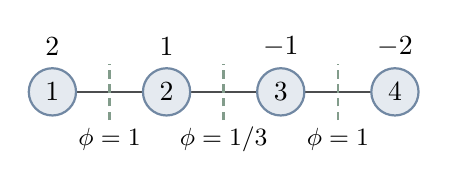
\begin{tikzpicture}[
  x=1.45cm,y=1cm,
  vertex/.style={circle,draw=graphSweepBlue,fill=graphSweepLight,
    line width=.8pt,minimum size=6mm,inner sep=0pt},
  cut/.style={draw=graphSweepGreen,densely dashed,line width=.85pt}
]
\definecolor{graphSweepBlue}{HTML}{7188A3}
\definecolor{graphSweepLight}{HTML}{E5EAF0}
\definecolor{graphSweepGreen}{HTML}{829C8B}
\definecolor{graphSweepLine}{HTML}{4C4D4F}
\draw[graphSweepLine,line width=.85pt] (0,0)--(3,0);
\foreach \i/\v/\f in {0/1/2,1/2/1,2/3/-1,3/4/-2}{
   \node[vertex] at (\i,0) {$\v$};
   \node at (\i,.57) {$\f$};
}
\foreach \i/\value in {.5/1,1.5/{1/3},2.5/1}{
   \draw[cut] (\i,-.36)--(\i,.35);
   \node[font=\small] at (\i,-.6) {$\phi=\value$};
}
\end{tikzpicture}

\caption{单位权四顶点路径上的阈值扫描。顶点上方标出了归一化谱方向还原后的函数值。三条竖虚线对应三个候选阈值，每个阈值恰好切过一条边。}
\label{fig:graph-cheeger-path-sweep}
\end{figure}

用四点路径验证。各点度为$(1,2,2,1)$。取$\bm f=(2,1,-1,-2)^\top$，计算
\[
\bm L\bm f=(1,1,-1,-1)^\top=\tfrac12\bm D\bm f,
\]
可知$\bm f$确实是归一化特征值$\mu_2=1/2$对应的方向。负值侧和正值侧的体积各为$3$，取中位数$\tau=0$后正部为$\bm g=(2,1,0,0)^\top$。

沿边能量为$(2-1)^2+(1-0)^2+(0-0)^2=2$，度加权平方和为$1\cdot4+2\cdot1=6$，能量商为$2/6=1/3<\mu_2$。

$g_i^2$的取值为$(4,1,0,0)$，产生两个非空阈值区间。图~\ref{fig:graph-cheeger-threshold-intervals}在同一条阈值轴上标出了顶点入选和边被切过的区间。

\begin{BookInlineFigure}
  \centering
  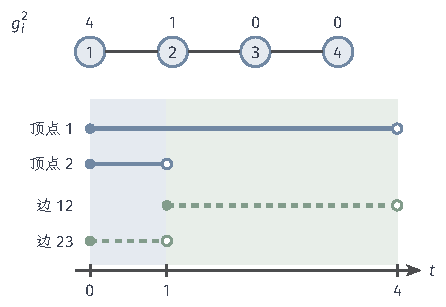
\includegraphics{figures/03-graphs/05-matrices-and-spectra/tikz/cheeger-threshold-intervals/figure.pdf}
  \caption{对$g_i^2=(4,1,0,0)_i$扫描阈值$t$。实线段标出顶点入选的区间，虚线段标出边跨割的区间。顶点$3,4$始终不入选，边$34$始终不被切过。}
  \label{fig:graph-cheeger-threshold-intervals}
\end{BookInlineFigure}

区间$[0,1)$选入$\{1,2\}$，体积$3$，割权$1$（边$23$被切），导通率$1/3$。区间$[1,4)$只选入$\{1\}$，体积$1$，割权$1$（边$12$被切），导通率$1$。

体积积分为$1\cdot3+3\cdot1=6$，割权积分为$1\cdot1+3\cdot1=4$。比值$4/6=2/3$，恰好位于两个导通率$1/3$和$1$之间。上界要求至少有一个候选不超过$\sqrt{2\cdot1/2}=1$，中间割的$1/3$远远满足。

直接按$\bm f$排序时，还有一个候选是$\{1,2,3\}$，它也只切过一条边，导通率为$1/3$。三个候选都只切一条边，中间位置的小侧体积最大，导通率最低。

\subsection{两端的紧性}
\label{sec:graph-cheeger-tightness}

Cheeger不等式的两端不能同时改进为同一个线性关系。下面通过两族图分别说明下界和上界各自的紧性。

\paragraph{下界取等：超立方体}

$d$维超立方体的$2^d$个顶点各有$d$条边，是$d$正则图。组合拉普拉斯的第二小特征值为$2$（沿任一坐标交替赋值$\pm1$给出这个值）。归一化后$\mu_2=2/d$。

沿某一坐标把顶点等分为两半。每个顶点恰有一条边跨割，每侧体积为$2^{d-1}\cdot d$。导通率为$2^{d-1}/(2^{d-1}\cdot d)=1/d$，恰好等于$\mu_2/2$。结合下界$\phi_*\geq\mu_2/2=1/d$，可以断定$\phi_*=1/d$。这说明下界的等号确实可以达到。

\paragraph{上界中的平方根尺度：长环}

对偶数$n\geq4$的环$C_n$，每个非平凡割至少切过两条边。取相邻的$n/2$个顶点为一侧，割权为$2$，该侧体积为$n/2\cdot 2=n$，导通率为$2/n$。可以验证这就是最小导通率$\phi_*=2/n$。

归一化拉普拉斯的第二小特征值为
\[
\mu_2=1-\cos(2\pi/n).
\]
当$n$增大时，$1-\cos(2\pi/n)\approx 2\pi^2/n^2$，因此$\mu_2$是$n^{-2}$阶的量，而$\phi_*=2/n$是$n^{-1}$阶的量。两者之间确实存在平方根的尺度差距：$\phi_*$与$\sqrt{\mu_2}$同阶。这说明上界$\phi_*\leq\sqrt{2\mu_2}$中的平方根不是证明技巧造成的损失，而是反映了长环这类图的真实结构。

这两族图放在一起看，下界可以精确取等，上界中的平方根指数不能改进。但两端并不在同一族图上同时取等——超立方体实现了下界的常数，长环展示了上界的指数。

\section{RatioCut谱划分}
\label{sec:graph-ratiocut}

给定一张图，要把顶点分成两个非空组。边的两个端点分在不同组时，需要付出这条边的权重。如果只求割权最小，把一个度最低的顶点单独切出来往往就够了，但这样的分组并不平衡。\term{RatioCut}用两侧的顶点数量调整割权，使得切出很小一组的方案被放大惩罚。

\subsection{RatioCut的谱松弛}
\label{sec:graph-ratiocut-relaxation}

设第一组为$S$，第二组为$\bar S=V\setminus S$，两组的顶点数分别为$s=|S|$和$t=|\bar S|$，满足$s+t=n$。将割权分别除以两组大小，再相加，定义
\begin{equation}
\label{eq:graph-ratiocut}
\operatorname{RatioCut}(S)=c(S,\bar S)\left(\frac{1}{s}+\frac{1}{t}\right).
\end{equation}
若两种切法的割权相同，其中一种只留下很小的一组，那个组对应的倒数$1/s$就会很大，整体代价随之增大。

在四点路径上，切下端点$1$得到一对三的分组，割权为$1$，代价为$1\cdot(1+1/3)=4/3$。切断中间边得到二对二的分组，割权也为$1$，代价为$1\cdot(1/2+1/2)=1$。中间割在RatioCut意义下更优。

目标是在所有非空二分中找出代价最小的分组。为了用拉普拉斯的谱工具求解，我们先把分组编码为一个向量。

给$S$上的顶点赋$1$，$\bar S$上的赋$0$，得到指示向量$\bm 1_S$。跨边的两端相差$1$，组内边的两端相差$0$，因此沿边能量$\bm 1_S^\top\bm L\bm 1_S$恰好等于割权$c(S,\bar S)$。

但这个向量的坐标和为$s$，不满足式~\eqref{eq:graph-algebraic-connectivity}的正交条件$\bm x\perp\bm 1$。将每个坐标减去均值$s/n$，得到
\[
\bm y=\bm 1_S-\frac{s}{n}\bm 1.
\]
$\bm y$在$S$上取$t/n$，在$\bar S$上取$-s/n$。两侧之差仍为$t/n-(-s/n)=1$，跨边的能量不变，组内边仍无贡献。因此$\bm y^\top\bm L\bm y=c(S,\bar S)$。

向量的长度平方按两侧计算：
\[
\bm y^\top\bm y
=s\left(\frac{t}{n}\right)^{\!2}+t\left(\frac{s}{n}\right)^{\!2}
=\frac{st}{n}.
\]
将$\bm y$归一化为$\bm x=\bm y/\|\bm y\|$，它的长度变为$1$，坐标和仍为$0$。能量被除以$\|\bm y\|^2=st/n$，得到
\[
\bm x^\top\bm L\bm x
=\frac{n}{st}\,c(S,\bar S)
=c(S,\bar S)\left(\frac{1}{s}+\frac{1}{t}\right)
=\operatorname{RatioCut}(S).
\]
最后一步用到$n/(st)=1/s+1/t$。这就解释了两组顶点数的倒数之和为什么会出现。

以四点路径的中间割为例，$s=t=2$，归一化后的向量为$(1/2,1/2,-1/2,-1/2)^\top$。唯一的非零边差等于$1$，能量为$1$，恰好等于这个割的RatioCut值。

到此为止，向量$\bm x$只能取由分组确定的两个值。这个离散限制使得问题在组合意义上是困难的。谱松弛去掉两值限制，只保留$\bm x\perp\bm 1$和$\|\bm x\|=1$这两个条件。松弛后的最小值就是组合拉普拉斯的第二小特征值$\lambda_2$。

原来的每个分组向量都满足这两个条件，因而$\lambda_2$不超过任何实际RatioCut值。它是离散最优值的一个下界。

图~\ref{fig:graph-ratiocut-relaxation}对比了实际分组和松弛解。中间割的两值向量只在一条边上有变化，所有能量集中在那里。松弛解允许数值在多条边上逐步过渡，沿边能量因此更小。

\begin{BookInlineFigure}
  \centering
  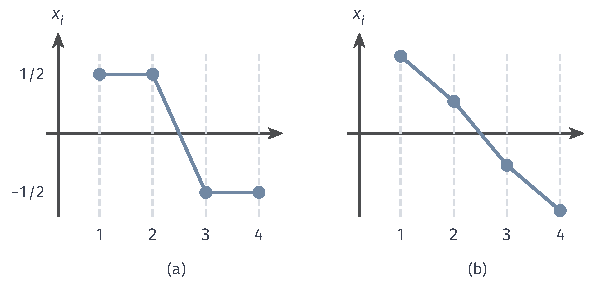
\includegraphics{figures/03-graphs/05-matrices-and-spectra/tikz/ratiocut-relaxation/figure.pdf}
  \caption{单位权四点路径的两种赋值。横轴按路径顺序标出顶点，纵轴是赋值。(a) 中间割的两值向量，能量为$1$。(b) 松弛后得到的第二特征向量，能量为$2-\sqrt2$。两者的坐标和都为零，长度都为一。}
  \label{fig:graph-ratiocut-relaxation}
\end{BookInlineFigure}

松弛给出了下界和一个连续方向，但这个方向本身不是合法的分组。下一步要把实数值的特征向量转换成可以在原图中使用的两组顶点。

\subsection{算法实现}
\label{sec:graph-ratiocut-sweep}

思路是按特征向量的分量从大到小排序，在相邻不同值之间逐个试切，并为每个候选分组计算原始的RatioCut目标。

\begin{algorithm}[RatioCut阈值扫描]
\label{alg:graph-ratiocut-sweep}
给定有限非负加权图，输出非空二分及其RatioCut值。
\begin{enumerate}
\item 若图不连通，选一个连通分量为一侧，另一侧为其余顶点。两侧之间没有正权边，割权为零，返回零代价的分组。
\item 否则求组合拉普拉斯的第二特征向量。按分量从大到小排序。分量相同的顶点作为一组，不能拆开。
\item 从空集开始逐组加入顶点。加入时更新割权：从当前割权中减去新顶点连向已选顶点的边权（这些边从跨边变为组内边），加上连向仍未入选顶点的边权（这些边从组内边变为跨边）。
\item 每组加入后，若两侧均非空，按式~\eqref{eq:graph-ratiocut}计算RatioCut。比较所有候选，返回目标值最小的分组。
\end{enumerate}
\end{algorithm}

\paragraph{执行过程}

在单位权四点路径上，第二特征向量可取为
\[
\bm x=(a,b,-b,-a)^\top,
\qquad a=\cos(\pi/8),\quad b=\cos(3\pi/8).
\]
因为$a>b>0$，顶点按$1,2,3,4$的顺序入选。

第一步放入顶点$1$。它只有一条边连向尚未入选的顶点$2$，割权变为$1$。第二步放入$2$时，边$12$从跨边变成组内边（割权减$1$），但边$23$从组内变为跨边（割权加$1$），割权仍为$1$。第三步放入$3$时，类似地跨边改成$34$。

三个候选的计算如下。
\begin{center}
\begin{tabular}{lccc}
\toprule
已选集合 & 两侧大小 & 割权 & RatioCut\\
\midrule
$\{1\}$ & $1,3$ & $1$ & $4/3$\\
$\{1,2\}$ & $2,2$ & $1$ & $1$\\
$\{1,2,3\}$ & $3,1$ & $1$ & $4/3$\\
\bottomrule
\end{tabular}
\end{center}

图~\ref{fig:ratiocut-sweep-candidates}按排序顺序画出四个顶点，并标出三种切分位置。每条竖线对应一种候选，线两侧的集合、割边及RatioCut值都标在旁边。观察中间切法如何同时使两侧大小均匀且割权不增。

\begin{figure}[!htb]
\centering
\begin{tikzpicture}[x=1mm,y=1mm,>=Stealth,
  vertex/.style={circle,draw=FigureBlue,fill=FigureBlueFill,inner sep=0pt,
    minimum size=5mm,line width=.52pt,font=\figurefont\fontsize{8}{10}\selectfont},
  cutline/.style={dashed,FigureRed,line width=.6pt},
  clabel/.style={font=\figurefont\fontsize{7}{8.5}\selectfont,FigureRed},
  vlabel/.style={font=\figurefont\fontsize{7.5}{9}\selectfont,FigureInk}]
  % vertices on a line
  \node[vertex] (v1) at (0,0) {$1$};
  \node[vertex] (v2) at (16,0) {$2$};
  \node[vertex] (v3) at (32,0) {$3$};
  \node[vertex] (v4) at (48,0) {$4$};
  \draw[FigureStroke,line width=.52pt] (v1)--(v2)--(v3)--(v4);
  % Cut 1: after vertex 1
  \draw[cutline] (8,7) -- (8,-7);
  \node[clabel,above] at (8,7.5) {$\frac{4}{3}$};
  % Cut 2: after vertex 2
  \draw[cutline] (24,7) -- (24,-7);
  \node[clabel,above] at (24,7.5) {$1$};
  % Cut 3: after vertex 3
  \draw[cutline] (40,7) -- (40,-7);
  \node[clabel,above] at (40,7.5) {$\frac{4}{3}$};
  % vertex ordering label
  \node[vlabel] at (24,-12) {按特征向量分量从大到小排序};
\end{tikzpicture}
\caption{四点路径上的RatioCut阈值扫描。四个顶点按第二特征向量分量递减排列。红色虚线标出三种切分位置，上方数字是对应的RatioCut值。中间割的代价最低。}
\label{fig:ratiocut-sweep-candidates}
\end{figure}

中间割的代价最小，为$1$。这是扫描得到的实际分组代价，可以和松弛下界$\lambda_2=2-\sqrt2\approx0.586$放在一起比较。

\subsection{算法分析}
\label{sec:graph-ratiocut-guarantee}

记所有非空二分中的RatioCut最小值为$\operatorname{OPT}_R$，扫描返回的分组为$S_R$。松弛扩大了可行域，给出下界；扫描提供了一个具体的可行割，给出上界：
\begin{equation}
\label{eq:graph-ratiocut-bounds}
\lambda_2\leq\operatorname{OPT}_R
\leq\operatorname{RatioCut}(S_R).
\end{equation}

四点路径上可以直接验证$\operatorname{OPT}_R=1$。任何非空二分至少切过一条边（路径是连通的），且两侧顶点数之积$st$至多为$\lfloor n/2\rfloor\cdot\lceil n/2\rceil=4$。因此$1/s+1/t=n/(st)\geq 4/4=1$，任何割的RatioCut都不低于$1$。中间割恰好达到了这个值。

排序$n$个顶点需要$O(n\log n)$时间。扫描过程中每个顶点加入一次，加入时检查它的邻接表，因此所有边在两个端点各被访问至多一次，扫描耗时$O(n+m)$。求特征向量的代价另行计算，取决于所用的迭代方法和精度要求。

一次扫描只比较沿一个排序方向切开的嵌套集合，没有覆盖全部$2^{n-1}-1$个无序二分。选择不同的最优方向（当$\lambda_2$为重根时）或近似方向可能给出不同的候选。相同分量作为一组处理，减少了切点数量。

精确的$\lambda_2$是有效的下界。但如果使用的是数值迭代得到的近似特征向量，代入Rayleigh商所得的值大于或等于$\lambda_2$，不一定仍是离散最优值的下界。报告结果时应区分：认证过误差的下界和数值估计值。扫描得到的分组及其原目标代价可以直接在原图上核对，不受特征向量精度的影响。

\section{NCut谱划分}
\label{sec:graph-ncut}

RatioCut在割权相同时偏好顶点数较均衡的划分，但顶点数不反映每个顶点参与连接的多少。例如，把星图的多个叶子归为一组，这组顶点内部没有边，其全部度数都来自跨组连接。若希望比较每侧跨组连接占该侧总连接量的比例，可以把分母换成集合体积。体积包括内部边和跨割边的贡献，不能直接等同于内部边权或内部连接密度。

为此，Shi与Malik于2000年提出将RatioCut分母中的“节点个数$|A|,|B|$”替换为子图中所有节点的\emph{度数之和}（即第~\ref{sec:graph-conductance}小节定义的集合体积$\operatorname{vol}(A),\operatorname{vol}(B)$），从而得到了\term{归一化割}（normalized cut，简称\term{NCut}）\scite{shi2000normalized}。

以下先限制在正度顶点集$V_+$上，并假定$V_+$非空；无自环图中这保证$|V_+|\geq2$。若全图没有正权边，则不存在两侧均为正体积的合法NCut划分。

\subsection{NCut的谱松弛}
\label{sec:graph-ncut-relaxation}

\begin{definition}[NCut目标]
\label{def:graph-ncut}
设非空二分$(A,B)$（其中$B=V\setminus A$）两侧的体积分别为$\operatorname{vol}(A)=\sum_{i\in A}d_i>0$和$\operatorname{vol}(B)=\sum_{j\in B}d_j>0$（满足$\operatorname{vol}(A)+\operatorname{vol}(B)=\operatorname{vol}(V)$）。划分$(A,B)$的归一化割（NCut）目标定义为
\begin{equation}
\label{eq:graph-ncut}
\operatorname{NCut}(A,B)
=\frac{c(A,B)}{\operatorname{vol}(A)}+\frac{c(A,B)}{\operatorname{vol}(B)}
=c(A,B)\left(\frac{1}{\operatorname{vol}(A)}+\frac{1}{\operatorname{vol}(B)}\right).
\end{equation}
\end{definition}

由$\operatorname{vol}(A)=2w(E(A))+c(A,B)$可得，当$c(A,B)/\operatorname{vol}(A)$较小时，$A$的度数总和主要来自内部边；另一侧同理。因此，NCut较小表示两侧各自只有较小比例的连接权重通向外部，并不保证内部连通或内部边密度较高。全图体积固定时，体积平衡也是目标的一部分，但不能同时独立最大化两侧体积。

\begin{BookInlineFigure}
  \centering
  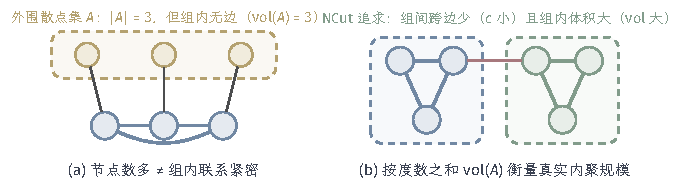
\includegraphics[width=114.935mm]{figures/03-graphs/05-matrices-and-spectra/tikz/ncut-volume-vs-count/figure.pdf}
  \caption{为什么NCut用度数总和（体积$\operatorname{vol}(A)$）替代节点个数$|A|$。(a) 将$3$个外围叶子归为集合$A$时，虽然节点数$|A|=3$已占半图，但$A$内部没有一条边，体积仅为$\operatorname{vol}(A)=3$。(b) 将两个内部紧密相连的三角形社区切开时，仅断开$1$条红边，而两侧体积各达$\operatorname{vol}=7$，两侧的跨割权与体积之比均为$1/7$。}
  \label{fig:graph-ncut-volume-vs-count}
\end{BookInlineFigure}

与第~\ref{sec:graph-ratiocut-relaxation}小节的RatioCut推导完全平行，只需把顶点个数$|A|,|B|$替换为集合体积$\operatorname{vol}(A),\operatorname{vol}(B)$，并把标准欧氏内积替换为以度矩阵$\bm D$加权的内积，即可分四步导出NCut的谱松弛。

\paragraph{1. 构造按体积加权的指示向量$\bm f$}

对任意满足$\operatorname{vol}(A)>0,\operatorname{vol}(B)>0$的二分$(A,B)$，利用两侧体积的比值构造两值指示向量$\bm f=(f_1,\ldots,f_n)^\top\in\mathbb R^n$：
\begin{equation}
\label{eq:ncut-indicator-vector}
  f_i = \begin{cases}
    \sqrt{\dfrac{\operatorname{vol}(B)}{\operatorname{vol}(A)}}, & i\in A,\\[10pt]
    -\sqrt{\dfrac{\operatorname{vol}(A)}{\operatorname{vol}(B)}}, & i\in B.
  \end{cases}
\end{equation}

\paragraph{2. 代入二次型分子$\bm f^\top\bm L\bm f$}

将$\bm f$代入组合拉普拉斯二次型$\bm f^\top\bm L\bm f=\sum_{\{i,j\}\in E}w_{i,j}(f_i-f_j)^2$。组内边两端取值相同、差为$0$；每条跨割边两端取值差的平方为
\[
\begin{aligned}
  \left(\sqrt{\frac{\operatorname{vol}(B)}{\operatorname{vol}(A)}} - \left(-\sqrt{\frac{\operatorname{vol}(A)}{\operatorname{vol}(B)}}\right)\right)^{\!2}
  &= \frac{\operatorname{vol}(B)}{\operatorname{vol}(A)} + \frac{\operatorname{vol}(A)}{\operatorname{vol}(B)} + 2 \\
  &= \operatorname{vol}(V)\left(\frac{1}{\operatorname{vol}(A)}+\frac{1}{\operatorname{vol}(B)}\right).
\end{aligned}
\]
对所有跨割边加权求和，得到二次型分子：
\begin{equation}
\label{eq:ncut-quadratic-numerator}
  \bm f^\top\bm L\bm f = \operatorname{vol}(V)\,c(A,B)\left(\frac{1}{\operatorname{vol}(A)}+\frac{1}{\operatorname{vol}(B)}\right)
  = \operatorname{vol}(V)\,\operatorname{NCut}(A,B).
\end{equation}

\paragraph{3. 验证度加权分母和度加权正交条件}

由于式~\eqref{eq:ncut-indicator-vector}使用的是体积比值，对应的正交条件和范数分母也自然带有顶点度数$d_i$的权重（即度对角矩阵$\bm D$）。第一，计算度加权坐标和$\bm f^\top\bm D\bm 1$：
\[
\begin{aligned}
  \bm f^\top\bm D\bm 1
  = \sum_{i=1}^n d_i f_i
  &= \left(\sum_{i\in A}d_i\right)\sqrt{\frac{\operatorname{vol}(B)}{\operatorname{vol}(A)}}
    - \left(\sum_{j\in B}d_j\right)\sqrt{\frac{\operatorname{vol}(A)}{\operatorname{vol}(B)}} \\
  &= \sqrt{\operatorname{vol}(A)\operatorname{vol}(B)} - \sqrt{\operatorname{vol}(A)\operatorname{vol}(B)}
  = 0.
\end{aligned}
\]
即向量$\bm f$恒满足度加权零和条件$\bm D\bm 1\perp\bm f$。

第二，计算度加权长度平方（分母$\bm f^\top\bm D\bm f$）：
\[
\begin{aligned}
  \bm f^\top\bm D\bm f
  = \sum_{i=1}^n d_i f_i^2
  &= \operatorname{vol}(A)\cdot\frac{\operatorname{vol}(B)}{\operatorname{vol}(A)}
    + \operatorname{vol}(B)\cdot\frac{\operatorname{vol}(A)}{\operatorname{vol}(B)} \\
  &= \operatorname{vol}(B) + \operatorname{vol}(A)
  = \operatorname{vol}(V).
\end{aligned}
\]
将分子式~\eqref{eq:ncut-quadratic-numerator}除以分母$\bm f^\top\bm D\bm f=\operatorname{vol}(V)$，常因子$\operatorname{vol}(V)$消去，得到广义Rayleigh商恒等式：
\begin{equation}
\label{eq:ncut-rayleigh-identity}
  \operatorname{NCut}(A,B) = \frac{\bm f^\top\bm L\bm f}{\bm f^\top\bm D\bm f}.
\end{equation}

\paragraph{4. 等价变换与连续松弛}

离散NCut问题要求$f_i$取式~\eqref{eq:ncut-indicator-vector}中由划分确定的两个值。放宽这一离散限制、允许$\bm f\in\mathbb R^n$取任意满足$\bm f^\top\bm D\bm 1=0$的非零实向量，并在正度顶点空间上作可逆坐标变换$\bm z=\bm D^{1/2}\bm f$（即$\bm f=\bm D^{-1/2}\bm z$），则正交约束$\bm f^\top\bm D\bm 1=0$化为$\bm z\perp\bm D^{1/2}\bm 1$，目标函数化为对称归一化拉普拉斯$\mathcal L=\bm D^{-1/2}\bm L\bm D^{-1/2}$的标准Rayleigh商：
\begin{equation}
\label{eq:ncut-spectral-relaxation}
  \min_{\substack{\bm f^\top\bm D\bm 1=0\\\bm f\neq\bm 0}}\frac{\bm f^\top\bm L\bm f}{\bm f^\top\bm D\bm f}
  = \min_{\substack{\bm z\perp\bm D^{1/2}\bm 1\\\bm z\neq\bm 0}}\frac{\bm z^\top\mathcal L\bm z}{\bm z^\top\bm z}
  = \mu_2(\mathcal L).
\end{equation}
由此可知：NCut连续松弛问题的最小值恰为对称归一化拉普拉斯的第二小特征值$\mu_2(\mathcal L)$；若达到$\mu_2(\mathcal L)$的特征向量为$\bm z_2$，则还原到原顶点空间的连续最优解为$\bm f^\star=\bm D^{-1/2}\bm z_2$，它直接满足广义特征方程$\bm L\bm f^\star=\mu_2\bm D\bm f^\star$（即随机游走归一化拉普拉斯特征方程$\bm L_{\mathrm{rw}}\bm f^\star=\mu_2\bm f^\star$）。

\begin{theorem}[NCut的度加权二次型表示与谱松弛下界]
\label{prop:graph-ncut-relaxation}
对任意两侧体积均为正的划分$(A,B)$，按式~\eqref{eq:ncut-indicator-vector}定义的指示向量$\bm f$（或其度加权单位化向量$\bm f_A=\bm f/\sqrt{\operatorname{vol}(V)}$）满足$\bm f^\top\bm D\bm 1=0$且$\operatorname{NCut}(A,B)=\frac{\bm f^\top\bm L\bm f}{\bm f^\top\bm D\bm f}$。因而，所有合法二分的离散最优值$\operatorname{OPT}_N=\min_{\operatorname{vol}(A),\operatorname{vol}(B)>0}\operatorname{NCut}(A,B)$以正度顶点集上对称归一化拉普拉斯$\mathcal L$的第二小特征值$\mu_2$为下界：
\[
  \mu_2(\mathcal L)
  = \min_{\substack{\bm f^\top\bm D\bm 1=0\\\bm f\neq\bm 0}}\frac{\bm f^\top\bm L\bm f}{\bm f^\top\bm D\bm f}
  = \min_{\substack{\bm z\perp\bm D^{1/2}\bm 1\\\lVert\bm z\rVert_2=1}}\bm z^\top\mathcal L\bm z
  \leq \operatorname{OPT}_N.
\]
\end{theorem}

注意$\mu_2$始终在正度顶点集$V_+=\{i\in V:d_i>0\}$上计算：度数为$0$的孤立顶点既不贡献割权也不贡献体积，可在正度顶点划分完毕后归入任意一侧。

\subsection{算法实现}
\label{sec:graph-ncut-sweep}

\paragraph{主要思路与算法步骤}

NCut谱划分的整体框架与RatioCut一致，核心差别在于将矩阵从组合拉普拉斯$\bm L$换成了对称归一化拉普拉斯$\mathcal L=\bm D^{-1/2}\bm L\bm D^{-1/2}$，并且在求得$\mathcal L$的特征向量$\bm z_2$后，必须左乘$\bm D^{-1/2}$作\emph{坐标逆缩放还原}，得到原顶点空间上的谱坐标$\bm f=\bm D^{-1/2}\bm z_2$后再执行排序或聚类。

具体执行流程分为以下四步：
\begin{enumerate}
\item \emph{构建归一化拉普拉斯矩阵}：在正度顶点集上计算对称归一化拉普拉斯矩阵$\mathcal L = \bm D^{-1/2}\bm L\bm D^{-1/2} = \bm I - \bm D^{-1/2}\bm W\bm D^{-1/2}$。
\item \emph{求解归一化特征向量}：计算$\mathcal L$的第二小特征值$\mu_2$对应的特征向量$\bm z_2\in\mathbb R^n$（若作$k$路谱聚类，则求$\mathcal L$前$k$个最小特征值对应的特征向量$\bm z_1,\bm z_2,\ldots,\bm z_k$）。
\item \emph{坐标逆缩放与构建特征矩阵}：在二分问题中，将特征向量$\bm z_2$的每个分量除以对应顶点度数的平方根$\sqrt{d_i}$，还原为原顶点指示空间上的谱坐标向量$\bm f=\bm D^{-1/2}\bm z_2$（即$f_i=(\bm z_2)_i/\sqrt{d_i}$）；在$k$路谱聚类（Ng--Jordan--Weiss算法）中，将$\bm D^{-1/2}[\bm z_1,\ldots,\bm z_k]$（或直接将$[\bm z_1,\ldots,\bm z_k]$）的每一行归一化为单位长度行向量，构建特征矩阵$\bm V\in\mathbb R^{n\times k}$。
\item \emph{离散化还原（还原为最终切分）}：在二分问题中，将全部顶点按还原后的坐标$f_i$从大到小排序，依次扫描$n-1$个前缀切口，计算各自的$\operatorname{NCut}(S,\bar S)$并取最小值对应的划分输出（在$k$路划分中则对特征矩阵$\bm V$的行向量运行$k$-means聚类）。
\end{enumerate}

\begin{algorithm}[NCut谱划分]
\label{alg:graph-ncut-sweep}
给定正度支撑非空且连通的有限无向非负加权图$\mathcal G=(V,E,w)$，输出两侧为正体积的二分$(A,B)$及其NCut值。
\begin{enumerate}
\item \textbf{构建归一化矩阵}：在正度支撑上构建对称归一化拉普拉斯矩阵$\mathcal L=\bm D^{-1/2}\bm L\bm D^{-1/2}$。
\item \textbf{求解特征向量并还原坐标}：求$\mathcal L$的第二小特征值$\mu_2$对应的特征向量$\bm z_2$，作逆缩放还原$\bm f=\bm D^{-1/2}\bm z_2$（即$f_i=(\bm z_2)_i/\sqrt{d_i}$）。
\item \textbf{按还原坐标排序}：按$f_i$从大到小排列顶点，分量值相同的并列顶点整组跨过阈值。
\item \textbf{离散化还原（增量阈值扫描）}：按排序顺序逐组将顶点并入前缀集合$S$，用算法~\ref{alg:graph-ratiocut-sweep}的方式增量更新割权$c(S,\bar S)$，同时累加集合体积$\operatorname{vol}(S)=\sum_{i\in S}d_i$。对所有两侧体积均为正的候选$S$，按式~\eqref{eq:graph-ncut}计算$\operatorname{NCut}(S,\bar S)$（同时可记录导通率$\phi(S)$），返回NCut最小的划分$(A,B)$，并把原图孤点归入任意一侧。
\end{enumerate}
\end{algorithm}

\paragraph{为什么必须用还原后的$f_i$排序？}

在第二步到第三步中，有一个极易忽略的关键细节：对称矩阵特征求解器算出的是$\bm z_2$，而我们在式~\eqref{eq:ncut-indicator-vector}中构造的两值分组向量是$\bm f=\bm D^{-1/2}\bm z_2$。由于不同顶点的度数$d_i$不同，除以$\sqrt{d_i}$可能会反转两个顶点的先后顺序。

图~\ref{fig:graph-ncut-coordinate-order}用一个简单例子展示了这种顺序反转：设圆点顶点的真实谱坐标为$f_1=2$、度数为$d_1=1$；方点顶点的真实谱坐标为$f_2=1$、度数为$d_2=9$。在乘以$\sqrt{d_i}$变换到$z_i=\sqrt{d_i}\,f_i$后，圆点坐标为$z_1=1\times 2=2$，而方点坐标变为$z_2=3\times 1=3$，大小顺序刚好颠倒。因此，阈值扫描必须严格使用逆缩放还原后的$f_i=(\bm z_2)_i/\sqrt{d_i}$排序（这与第~\ref{sec:graph-cheeger-sweep}小节Cheeger上界证明中的排序完全一致）。

\begin{BookInlineFigure}
  \centering
  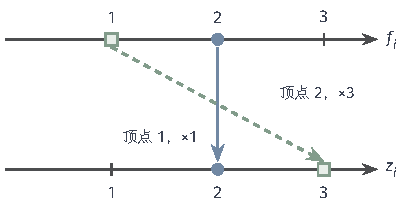
\includegraphics{figures/03-graphs/05-matrices-and-spectra/tikz/ncut-coordinate-order/figure.pdf}
  \caption{度数缩放可能改变顶点的排序先后。圆点对应度数$d_1=1$的顶点，方点对应度数$d_2=9$的顶点。按$z_i=\sqrt{d_i}\,f_i$转换到下轴时，方点坐标从$1$放大为$3$并反超圆点。阈值扫描必须使用上方的还原坐标$f_i$轴。}
  \label{fig:graph-ncut-coordinate-order}
\end{BookInlineFigure}

在单位权四点路径$1\!-\!2\!-\!3\!-\!4$上，各点度数为$(1,2,2,1)$，还原后的特征向量为$\bm f=(2,1,-1,-2)^\top$，按$f_i$从大到小排序仍为$1,2,3,4$。三个前缀候选切口的指标如下：切下$\{1\}$时割权为$1$、两侧体积为$1$和$5$，$\operatorname{NCut}=1\times(1+\frac15)=\frac65$；切断中间边得$\{1,2\}$时割权为$1$、两侧体积均为$3$，$\operatorname{NCut}=1\times(\frac13+\frac13)=\frac23$；切出$\{1,2,3\}$时$\operatorname{NCut}=\frac65$。算法返回中间割$\{1,2\}\mid\{3,4\}$，其NCut值$\frac23$夹在松弛下界$\mu_2=\frac12$之上。

\subsection{算法分析}
\label{sec:graph-ncut-guarantee}

记全图所有合法二分中的NCut真实最小值为$\operatorname{OPT}_N$，算法~\ref{alg:graph-ncut-sweep}扫描输出的划分为$S_N$。与RatioCut类似，松弛值$\mu_2$给出下界，扫描结果给出可行上界：
\begin{equation}
\label{eq:graph-ncut-bounds}
\mu_2(\mathcal L)\leq\operatorname{OPT}_N\leq\operatorname{NCut}(S_N,\bar S_N).
\end{equation}

NCut的松弛与阈值扫描使用的算子和坐标，与Cheeger不等式上界证明中的对象相同。由此可以得到不显式含最大度或最小度的目标值上界。下面分别核对目标函数、松弛方向和候选割之间的关系。

\paragraph{1. 目标函数同源：NCut与导通率$\phi(S)$仅差至多$2$倍}

对任意非空真子集$S\subsetneq V$，设两侧体积分别为$a=\operatorname{vol}(S)$和$b=\operatorname{vol}(\bar S)$，且不妨设$a\leq b$（即$a=\min\{\operatorname{vol}(S),\operatorname{vol}(\bar S)\}$）。对比定义~\ref{def:graph-conductance}与定义~\ref{def:graph-ncut}：
\[
\operatorname{NCut}(S,\bar S)
=\frac{c(S,\bar S)}{a}+\frac{c(S,\bar S)}{b}
=\frac{c(S,\bar S)}{a}\left(1+\frac{a}{b}\right)
=\phi(S)\left(1+\frac{a}{b}\right).
\]
由于$0<a\leq b$，比值$\frac{a}{b}$必定落在$(0,1]$内，故$1<\left(1+\frac{a}{b}\right)\leq 2$。因此，对图上的任何一个割，NCut与导通率$\phi(S)$都被锁定在常数$2$倍以内：
\begin{equation}
\label{eq:ncut-conductance-equivalence}
\phi(S)\leq\operatorname{NCut}(S,\bar S)\leq 2\phi(S).
\end{equation}

\paragraph{2. 谱松弛与扫描顺序完全一致}

对比式~\eqref{eq:graph-normalized-variational-cut}与式~\eqref{eq:ncut-spectral-relaxation}可以看到：Cheeger不等式所用的特征值$\mu_2(\mathcal L)$，与NCut连续谱松弛得到的下界$\mu_2(\mathcal L)$是\emph{同一个特征值}；而且第~\ref{sec:graph-cheeger-sweep}小节证明Cheeger上界时所扫描的特征向量$\bm f=\bm D^{-1/2}\bm z_2$，与算法~\ref{alg:graph-ncut-sweep}第三步排序所用的还原向量$\bm f=\bm D^{-1/2}\bm z_2$也是\emph{同一个向量}。换言之，NCut阈值扫描所考察的至多$|V_+|-1$个阈值前缀候选集，与Cheeger不等式上界证明所考察的前缀候选集完全相同。

\paragraph{3. 由Cheeger不等式直接导出NCut的性能保证}

由第~\ref{sec:graph-cheeger-sweep}小节的证明，同一批前缀候选中存在$S_\phi$使$\phi(S_\phi)\leq\sqrt{2\mu_2}$。算法在这些候选中最小化NCut，故$\operatorname{NCut}(S_N,\bar S_N)\leq\operatorname{NCut}(S_\phi,\bar S_\phi)$。再用$\operatorname{NCut}(S_\phi,\bar S_\phi)\leq2\phi(S_\phi)$和松弛下界$\mu_2\leq\operatorname{OPT}_N$，得到
\begin{equation}
\label{eq:graph-ncut-sweep-bound}
\begin{aligned}
\mu_2(\mathcal L)
&\leq \operatorname{OPT}_N
\leq \operatorname{NCut}(S_N,\bar S_N)
\leq \operatorname{NCut}(S_\phi,\bar S_\phi) \\
&\leq 2\phi(S_\phi)
\leq 2\sqrt{2\mu_2(\mathcal L)}
\leq 2\sqrt{2\operatorname{OPT}_N}.
\end{aligned}
\end{equation}

式~\eqref{eq:graph-ncut-sweep-bound}给出平方根形式的目标值保证。若$\operatorname{OPT}_N>0$，相除得到的近似因子为$2\sqrt{2/\operatorname{OPT}_N}$，并非常数；因此不能由此推断NCut在所有任务上优于RatioCut。得到准确谱向量后，排序与增量扫描共需$O(n\log n+m)$时间，特征向量求解的成本须另计。对于近似特征向量，还需根据其Rayleigh商和正交误差重新核对保证。

\begin{BookInlineFigure}
  \centering
  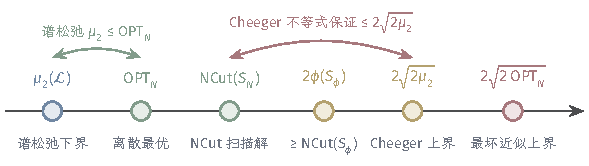
\includegraphics[width=99.713mm]{figures/03-graphs/05-matrices-and-spectra/tikz/ncut-sweep-and-cheeger-chain/figure.pdf}
  \caption{NCut谱划分与Cheeger不等式结合形成的双向近似保证链。左侧由连续谱松弛给出下界$\mu_2(\mathcal L)\leq\operatorname{OPT}_N$，右侧由Cheeger阈值扫描上界保证扫描输出解$S_N$满足$\operatorname{NCut}(S_N)\leq 2\sqrt{2\mu_2}\leq 2\sqrt{2\operatorname{OPT}_N}$。}
  \label{fig:graph-ncut-sweep-guarantee}
\end{BookInlineFigure}

\section{谱划分方法的比较}
\label{sec:graph-spectral-partition-comparison}

RatioCut与NCut同属基于拉普拉斯二次型松弛的谱划分方法，两者的算法骨架高度一致，核心区别仅在于\emph{如何定义子图的规模}：RatioCut按“顶点个数$|A|$”计规模，追求两侧节点数量的均衡；NCut按“度数总和（体积$\operatorname{vol}(A)$）”计规模，衡量跨割权相对于两侧总度数的比例。表~\ref{tab:ratiocut-vs-ncut}汇总了两种方法在各个环节的一一对应关系。

\begin{table}[!htb]
\centering
\caption{RatioCut与NCut谱划分方法的核心要素对比。}
\label{tab:ratiocut-vs-ncut}
\footnotesize
\begin{tabular}{lll}
\toprule
对比维度 & RatioCut（比例割） & NCut（归一化割）\\
\midrule
均衡目标 & 节点个数$|A|,|B|$均衡 & 度体积$\operatorname{vol}(A),\operatorname{vol}(B)$均衡\\
目标函数 & $c(A,B)\bigl(\frac{1}{|A|}+\frac{1}{|B|}\bigr)$ & $c(A,B)\bigl(\frac{1}{\operatorname{vol}(A)}+\frac{1}{\operatorname{vol}(B)}\bigr)$\\
两值向量$f_i$ & $\sqrt{|B|/|A|},-\sqrt{|A|/|B|}$ & 式~\eqref{eq:ncut-indicator-vector}的两值\\
等价Rayleigh商 & $\dfrac{\bm f^\top\bm L\bm f}{\bm f^\top\bm f}$ & $\dfrac{\bm f^\top\bm L\bm f}{\bm f^\top\bm D\bm f}$\\
松弛算子 & 组合拉普拉斯$\bm L=\bm D-\bm W$ & 对称归一化$\mathcal L=\bm D^{-1/2}\bm L\bm D^{-1/2}$\\
下界与排序 & $\lambda_2(\bm L)$，按$\bm v_2$排序 & $\mu_2(\mathcal L)$，按$\bm f=\bm D^{-1/2}\bm z_2$排序\\
Cheeger保证 & 需另行给出相应尺度的界 & $\operatorname{NCut}(S_N)\leq 2\sqrt{2\operatorname{OPT}_N}$\\
\bottomrule
\end{tabular}
\end{table}

在正则图上，两种目标成比例；度数不完全相同时，即使差异较小，也不能保证最优划分一致。下面通过一个具体的四点加权路径算例直观展示这一分歧。

\paragraph{加权路径上的最优割分歧}

考虑图~\ref{fig:graph-partition-weighted-path}所示的四顶点路径$1\!-\!2\!-\!3\!-\!4$，将其三条边的权重设为中间重、两端轻：$w_{12}=1$，$w_{23}=2$，$w_{34}=1$。由此算出四个顶点的加权度依次为$d_1=1,d_2=3,d_3=3,d_4=1$，全图总体积为$\operatorname{vol}(V)=8$。

\begin{BookInlineFigure}
  \centering
  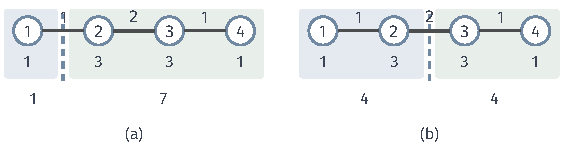
\includegraphics{figures/03-graphs/05-matrices-and-spectra/tikz/partition-weighted-path/figure.pdf}
  \caption{加权路径（边权$1,2,1$）上的两个关键候选割。(a) 切下左端点$1$：只切断权重为$1$的端边，两侧顶点数为$1$对$3$，两侧体积为$1$对$7$。(b) 沿中间边切开：需切断权重为$2$的粗边，但两侧顶点数（$2$对$2$）与体积（$4$对$4$）均相等。顶点下方标注加权度。}
  \label{fig:graph-partition-weighted-path}
\end{BookInlineFigure}

我们重点比较图~\ref{fig:graph-partition-weighted-path}标出的两种切法：
\begin{enumerate}
\item \emph{候选一：切下低度端点$\{1\}\mid\{2,3,4\}$}（图a，与切下右端点$\{4\}\mid\{1,2,3\}$对称）。这一刀避开了中间权重为$2$的粗边，只切断权重为$1$的轻边$12$，故割权$c=1$。两侧的节点个数为$|A|=1,|B|=3$，而两侧的体积则悬殊为$\operatorname{vol}(A)=1,\operatorname{vol}(B)=7$。代入两个目标函数：
\[
\begin{aligned}
  \operatorname{RatioCut}(\{1\}) &= 1\times\left(\frac{1}{1}+\frac{1}{3}\right) = \frac{4}{3}\approx 1.333, \\
  \operatorname{NCut}(\{1\}) &= 1\times\left(\frac{1}{1}+\frac{1}{7}\right) = \frac{8}{7}\approx 1.143.
\end{aligned}
\]
\item \emph{候选二：切断中间重边$\{1,2\}\mid\{3,4\}$}（图b）。这一刀直接切断权重为$2$的中间边$23$，割权升至$c=2$，但换来了两侧规模相等——两侧节点个数为$2$对$2$，两侧体积均为$1+3=4$。代入两个目标函数：
\[
  \operatorname{RatioCut}(\{1,2\}) = 2\times\left(\frac{1}{2}+\frac{1}{2}\right) = 2,
  \qquad
  \operatorname{NCut}(\{1,2\}) = 2\times\left(\frac{1}{4}+\frac{1}{4}\right) = 1.
\]
\end{enumerate}

至于其余非空二分（如将两端点合为一组的$\{1,4\}\mid\{2,3\}$，或奇偶交错的$\{1,3\}\mid\{2,4\}$），它们同时切断了两条或三条边，割权不低于$2$且规模不比中间割更优。图~\ref{fig:graph-comparison-four-bipartitions}与下表展示了四类代表性二分；下表还列出了切下内部顶点的第五类，从而覆盖所有非空二分（对称情形合并）的结构与指标：

\begin{BookInlineFigure}
  \centering
  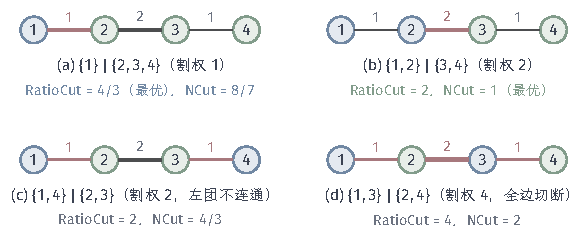
\includegraphics[width=98.316mm]{figures/03-graphs/05-matrices-and-spectra/tikz/comparison-four-bipartitions/figure.pdf}
  \caption{加权路径（边权$1,2,1$）的四类非空二分结构对比。蓝色与绿色区分两侧子集，红色边表示被切断的跨割边。(a) 切下单个端点，RatioCut达到全局最小$4/3$；(b) 切断中间重边，NCut达到全局最小$1$；(c) 两端点合并为一侧，同时切断两条端边且左侧不连通；(d) 奇偶交错分组，三条边全部被切断。}
  \label{fig:graph-comparison-four-bipartitions}
\end{BookInlineFigure}
\begin{center}
\small
\setlength{\tabcolsep}{4pt}
\begin{tabular}{lccccc}
\toprule
候选划分 & 割权$c$ & 节点数 & 两侧体积 & RatioCut & NCut\\
\midrule
$\{1\}\mid\{2,3,4\}$ & $1$ & $1,3$ & $1,7$ & $\mathbf{4/3}$ & $8/7$\\
$\{1,2\}\mid\{3,4\}$ & $2$ & $2,2$ & $4,4$ & $2$ & $\mathbf{1}$\\
$\{2\}\mid\{1,3,4\}$ & $3$ & $1,3$ & $3,5$ & $4$ & $8/5$\\
$\{1,4\}\mid\{2,3\}$ & $2$ & $2,2$ & $2,6$ & $2$ & $4/3$\\
$\{1,3\}\mid\{2,4\}$ & $4$ & $2,2$ & $4,4$ & $4$ & $2$\\
\bottomrule
\end{tabular}
\end{center}

枚举全部二分后，RatioCut的最小值为$4/3$，由两种端点割取得；NCut的最小值为$1$，由中间割取得。端点割将割权从$2$减为$1$，足以抵消RatioCut中的顶点数失衡代价；在NCut中，端点仅占总体积的$1/8$，其代价$8/7$仍大于中间割的$1$。这一差异来自两个目标采用的规模度量。

\paragraph{正则图上的统一性与实践选择建议}

当图是加权度恒为常数$d>0$的$d$正则图时，任意子集$A$的体积恒等于节点数的$d$倍：$\operatorname{vol}(A)=d|A|$。此时NCut与RatioCut严格成正比：
\[
\operatorname{NCut}(A,B)
=c(A,B)\left(\frac{1}{d|A|}+\frac{1}{d|B|}\right)
=\frac{1}{d}\operatorname{RatioCut}(A,B),
\]
对称归一化拉普拉斯也简化为$\mathcal L=\frac{1}{d}\bm L$，两种离散目标具有相同的最优划分。若选择相同的特征方向并使用一致的并列处理规则，谱扫描的排序与结果也相同；重特征值或多个最优切口可能使不同实现返回不同划分。

选择目标应依据任务如何衡量规模。若每个顶点代表等量负载，可以考虑RatioCut；若关心每侧跨组连接占总连接量的比例，可以考虑NCut。二者都是软性的均衡目标，均不保证指定的组大小或内部密度。若任务要求严格等分，应另加规模约束，并重新分析算法和保证。

\section{本章小结}
\label{sec:graph-spectral-partition-summary}

组合拉普拉斯的第二小特征值$\lambda_2$衡量连通图连得有多紧。它不低于点连通度和边连通度（对简单无权非完全图），Fiedler向量的非负一侧在连通图上保持连通。但$\lambda_2$会随边权整体放大而增大，跨图比较时需要消除尺度。

归一化拉普拉斯的第二小特征值$\mu_2$用度加权长度替代普通长度。Cheeger不等式把$\mu_2$与最小导通率$\phi_*$从两侧绑在一起：下界$\mu_2/2\leq\phi_*$说明图中不存在太稀疏的平衡割，上界$\phi_*\leq\sqrt{2\mu_2}$提供了一个构造性的搜索——按特征方向排序并扫描阈值，其中至少一个割满足导通率保证。超立方体实现了下界等号，长环展示了上界中平方根尺度的必要性。

实际分组只给顶点两种值。RatioCut用顶点数计量组规模，松弛为$\lambda_2$的变分问题。NCut用度的总和计量，松弛为$\mu_2$的变分问题。两者的流程相同：求特征向量、排序、逐阈值扫描、按原目标选出最优候选。松弛值是离散最优值的下界，扫描候选给出上界，两者合在一起为分组质量提供可核验的区间。

这些步骤反复用到拉普拉斯的二次型。下一章研究怎样用更少的边同时近似保留所有顶点方向上的能量，并将这种稀疏近似用于方程求解。


\chapter{图的稀疏化}
\label{chap:graph-sparsification}

在前面两章的拉普拉斯方程迭代求解与谱划分中，每计算一次拉普拉斯矩阵与向量的乘积$\bm L\bm x$，都要遍历图中的所有$m$条边。当原图$\mathcal G$是边数高达$\Theta(n^2)$的稠密图时，矩阵乘法每次需要$O(n^2)$时间。如果能用一张共享同一顶点集$V$、但边数仅有$O(n\log n/\varepsilon^2)$的稀疏重加权子图$\mathcal H$来代替原图$\mathcal G$，对$\mathcal H$的矩阵乘法只需按其边数计时；能否加速原问题，还取决于近似误差、构造成本与后续算法。

然而，简单地随机删边很容易破坏图的关键结构：设两个稠密大团之间仅靠一条细桥相连，一旦删边时漏掉了这条桥，两团之间的割权会从正数降为零，图由连通变为不连通；相反，若删去的是稠密团内部的一条边，由于两端顶点之间还有大量并联替代路径，可以尝试通过保留边重加权控制误差，但仍须验证谱近似条件。

这一对比说明，构造稀疏图必须回答三个核心问题：第一，什么样的替代图$\mathcal H$才算在数学上严格逼近了原图$\mathcal G$？第二，应当按什么概率抽取原图的边、并如何重新分配权重，才能既保留关键瓶颈边又大幅削减冗余边？第三，如何利用构造出的稀疏图加速原图拉普拉斯方程的求解？

本章讨论无向无自环图，设原图$\mathcal G=(V,E,c)$包含$n=|V|\geq 2$个顶点和$m=|E|$条正权边，替代图$\mathcal H=(V,E_H,\widehat c)$保留全部顶点并从$E$中选取子集重新赋权。对每条边$e=\{u,v\}\in E$，固定任意参考方向并记边关联向量为$\bm b_e=\bm e_u-\bm e_v\in\mathbb R^n$，则顶点赋值向量$\bm x\in\mathbb R^n$在原图与替代图上的拉普拉斯二次型分别为
\[
\bm x^\top\bm L_G\bm x
=\sum_{e\in E}c_e(\bm b_e^\top\bm x)^2,
\qquad
\bm x^\top\bm L_H\bm x
=\sum_{e\in E_H}\widehat c_e(\bm b_e^\top\bm x)^2.
\]
第~\ref{sec:graph-sparsification-approximation}节首先定义割近似与谱近似，说明谱近似对线性求解所提供的额外控制，并分别证明谱近似保持特征值、有效电阻与方程解的三条核心性质；第~\ref{sec:graph-resistance-sampling}节直接调用第~\ref{sec:graph-sparsification-resistance-trees}小节的生成树包含概率与Foster定理，给出基于有效电阻抽样的稀疏图构造算法与矩阵Chernoff界证明；第~\ref{sec:graph-sparse-preconditioning}节展示如何将稀疏图作为预条件子加速原图拉普拉斯方程的共轭梯度求解。

\section{割近似与谱近似}
\label{sec:graph-sparsification-approximation}

稀疏化的目标是用一张边少得多的图来代替原图。但代替到什么程度才算够用？本节先从割权开始回答这个问题，再把要求提高到所有实值向量上的能量。

\subsection{割近似}
\label{sec:graph-cut-approximation}

假设原来某个割的权是十。如果允许百分之十的误差，替代图上这个割的权落在九和十一之间就算可以接受。如果原来的割权为零，相对误差要求替代图上也是零——两团之间没边的判断不能弄错。

但是，稀疏化是在看到任何特定的割之前就已经选定了一张替代图。之后在替代图上搜索最小割时，算法会逐一比较各种分组，其中可能恰好有一种分组的跨边被删掉了许多。因此我们要求先固定替代图，再让它对\emph{每一个}分组都满足同一个相对误差。

\begin{definition}[割近似]
\label{def:graph-cut-approximation}
设$\mathcal G$与$\mathcal H$有同一顶点集$V$，$0<\varepsilon<1$。对$S\subseteq V$，记$\overline S=V\setminus S$，用$c_G(S,\overline S)$和$c_H(S,\overline S)$分别表示两图中跨越该割的边权之和。若每个$S$都满足
\begin{equation}
(1-\varepsilon)c_G(S,\overline S)
\leq c_H(S,\overline S)
\leq (1+\varepsilon)c_G(S,\overline S),
\label{eq:graph-cut-approximation}
\end{equation}
就说$\mathcal H$是$\mathcal G$的一个$\varepsilon$\term{割近似}（cut approximation）。
\end{definition}

下界系数$1-\varepsilon$是正数，所以原图中有正权边跨越的割，在$\mathcal H$中仍有正权边跨越。零割也自动保持为零。这保证了"某一组顶点与外部是否相连"的判断不变。

\paragraph{最小割的继承}

记$C_G$和$C_H$为两图的最小割权。两图的分组候选完全相同，但取到最小值的分组可能不同。

先给$C_H$找一个下界。设$S^*_H$是$\mathcal H$中的最优分组，按割近似的上界，它在$\mathcal H$中的割权至多是它在$\mathcal G$中割权的$1+\varepsilon$倍。反过来，$\mathcal G$中的最优分组$S^*_G$作为$\mathcal H$的一个候选，其在$\mathcal H$中的割权至少是在$\mathcal G$中的$1-\varepsilon$倍。$\mathcal H$的最小割不超过任何候选，$\mathcal G$的最小割不超过$S^*_H$在$\mathcal G$上的值，因此
\begin{equation}
(1-\varepsilon)C_G\leq C_H\leq(1+\varepsilon)C_G.
\label{eq:graph-sparsification-min-cut}
\end{equation}

\paragraph{RatioCut的继承}

第~\ref{chap:spectral-partition}章的RatioCut把割权乘以$1/|S|+1/|\overline S|$。两图共享同一个顶点集，因此这个因子在每个割上完全相同。割权的$1\pm\varepsilon$比例直接传给了RatioCut的目标值，最优值也是如此。

\paragraph{体积和导通率的继承}

导通率和NCut还用到集合的\emph{体积}，即一侧顶点的加权度之和$\operatorname{vol}_G(S)=\sum_{i\in S}d_i$。换了边权后，各顶点的加权度也会改变。

取单点集合$\{v\}$。它的割恰好由$v$的所有关联边组成，因此式~\eqref{eq:graph-cut-approximation}也控制了每个顶点的加权度。将组内所有顶点的度下界相加或上界相加，得到
\begin{equation}
(1-\varepsilon)\operatorname{vol}_G(S)
\leq \operatorname{vol}_H(S)
\leq (1+\varepsilon)\operatorname{vol}_G(S).
\label{eq:graph-sparsification-volume}
\end{equation}
需要注意的是，组内边在组内两个顶点的度里各计一次，但在$S$的割权中不出现。

第~\ref{sec:graph-cheeger}节的导通率以割权为分子、以较小一侧的体积为分母。分子和分母都可能偏离原值。用割权下界除以体积上界，可以得到导通率的下界；用割权上界除以体积下界，得到上界。记两图的导通率为$\phi_G(S)$和$\phi_H(S)$，整理后
\begin{equation}
\frac{1-\varepsilon}{1+\varepsilon}\phi_G(S)
\leq \phi_H(S)
\leq \frac{1+\varepsilon}{1-\varepsilon}\phi_G(S).
\label{eq:graph-sparsification-conductance}
\end{equation}
NCut是割权分别除以两侧体积之后的和。每一项都继承同样的比例界，两图的正体积集合相同，因此可以在相同的合法划分上取最小来比较最优值。

\subsection{谱近似}
\label{sec:graph-spectral-approximation}

割近似只看指示向量——每个顶点要么在$S$中取一、要么在$\overline S$中取零。这时跨割边两端的差平方都是一，能量就等于跨割的边权之和。

但谱划分的松弛和拉普拉斯方程用到的是\emph{任意实值}的顶点赋值。两端相差五的那条边和两端相差零点一的那条边，对能量的贡献可以差几个数量级。单纯比较跨边总权看不出重加权集中在差异大的边还是差异小的边。因此需要一种更严格的保证：让替代图在\emph{每一种}赋值上的能量都接近原图。

\begin{definition}[谱近似]
\label{def:graph-spectral-approximation}
设$\bm L_G$和$\bm L_H$是同一顶点集上两图的拉普拉斯矩阵。若对每个$\bm x\in\mathbb R^n$都有
\begin{equation}
(1-\varepsilon)\bm x^\top\bm L_G\bm x
\leq \bm x^\top\bm L_H\bm x
\leq (1+\varepsilon)\bm x^\top\bm L_G\bm x,
\label{eq:graph-spectral-approximation-energy}
\end{equation}
则称$\mathcal H$是$\mathcal G$的一个$\varepsilon$\term{谱近似}（spectral approximation）。用半正定序写，就是
\begin{equation}
(1-\varepsilon)\bm L_G\preceq\bm L_H\preceq(1+\varepsilon)\bm L_G.
\label{eq:graph-spectral-approximation-order}
\end{equation}
边数显著减少且满足此条件的构造称为\term{谱稀疏化}（spectral sparsification）。
\end{definition}

谱近似蕴含割近似。只需在式~\eqref{eq:graph-spectral-approximation-energy}中把$\bm x$取成子集$S$的指示向量——只有跨割边的两端值不同，差的平方都是一，因此能量恰好等于割权。代入后就得到式~\eqref{eq:graph-cut-approximation}。

谱近似还自动保留连通分量。若$\bm x^\top\bm L_G\bm x=0$，上界迫使$\bm x^\top\bm L_H\bm x=0$。反过来，若$\bm x^\top\bm L_H\bm x=0$，正的下界系数$1-\varepsilon$迫使原图能量也为零。第~\ref{sec:graph-laplacian-kernel}节说过，能量为零要求在每个正权连通分量上取常值。因此两图的零能量方向完全相同，连通分量也完全相同。

对连通图，只有常值方向的能量为零。在$\bm 1^\perp$中，非零向量的能量为正，可以取拉普拉斯的逆。

\paragraph{割近似不蕴含谱近似}

反过来的推论不成立。下面用一个三顶点的例子说明，满足割近似的替代图在某个实值向量上的能量可以超出谱近似的允许范围。

\begin{example}[满足割界的图可以超出同一谱界]
\label{ex:graph-cut-not-spectral}
令$\mathcal G$是单位权三角形，三条边的权都是一。取$0<\varepsilon<1/2$，构造替代图$\mathcal H$：把边$12$的权增加$2\varepsilon$，把边$23$的权减少$2\varepsilon$，边$13$保持不变，
\[
c_H(12)=1+2\varepsilon,\qquad c_H(23)=1-2\varepsilon,\qquad c_H(13)=1.
\]

先检查割近似。原图中每个顶点都连着两条单位权边，三个单点割的权都是二。替代图中：顶点$1$的两条边权之和为$(1+2\varepsilon)+1=2+2\varepsilon$，顶点$2$的为$(1+2\varepsilon)+(1-2\varepsilon)=2$，顶点$3$的为$(1-2\varepsilon)+1=2-2\varepsilon$。三个数都落在$2(1\pm\varepsilon)$之间。因为两点割和它的单点补割权相同，所以全部六个非平凡割都满足式~\eqref{eq:graph-cut-approximation}。

再取顶点赋值$\bm x=(3,-2,-1)^\top$。三条边上两端差的平方分别是
\[
(3-(-2))^2=25,\qquad ((-2)-(-1))^2=1,\qquad (3-(-1))^2=16.
\]
原图能量为$25+1+16=42$。替代图的能量为
\[
25(1+2\varepsilon)+1\cdot(1-2\varepsilon)+16\cdot1=42+48\varepsilon.
\]
比如取$\varepsilon=1/4$。此时所有割权都在原值的$75\%$到$125\%$之间——割近似完全满足。但这个向量的能量从$42$升到了$54$，超过了谱近似允许的上界$42\times 5/4=52.5$。

能量比为$1+48\varepsilon/42=1+8\varepsilon/7$，严格大于$1+\varepsilon$。原因在于：顶点$2$的单点割看到的两条边权一增一减，总和不变。但这个实值赋值在边$12$上的差平方为$25$，在边$23$上只有$1$，增权集中在能量高的边上，减权集中在能量低的边上，二者无法对消。图~\ref{fig:sparsification-cut-energy}并排画出两图和同一个赋值，便于逐边比较。
\end{example}

\begin{BookInlineFigure}
  \centering
  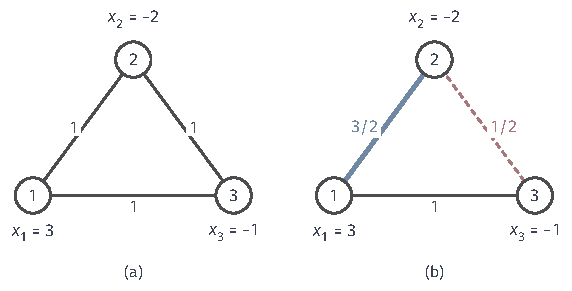
\includegraphics{figures/03-graphs/05-matrices-and-spectra/tikz/sparsification-cut-energy/figure.pdf}
  \caption{单位权原图（a）和取$\varepsilon=1/4$的替代图（b）。粗实线表示增重的边，虚线表示减重的边。三个单点割的权都满足$1\pm\varepsilon$比例，但按相同的顶点赋值$(3,-2,-1)$计算能量，替代图从$42$升到$54$，超出了谱近似的允许范围。}
  \label{fig:sparsification-cut-energy}
\end{BookInlineFigure}


\subsection{谱近似保持的量}
\label{sec:graph-spectral-approximation-consequences}

有了谱近似图，可以用它来估计原图的特征值、有效电阻和方程解。这三种比较共用同一个能量界，但各自控制的量不同：特征值来自能量商的极值，后两种还需要把比较从拉普拉斯传到逆矩阵上。

\paragraph{特征值的保持}

先把两图的组合拉普拉斯特征值各按从小到大排序。对每个$i$，想要比较第$i$个特征值。

式~\eqref{eq:graph-spectral-approximation-energy}对每个非零向量成立，两边同除以$\bm x^\top\bm x$仍然成立。左边和右边变成了Rayleigh商的比例界。在同一个$i$维子空间上分别对两图取商的最大值，原来的比例界不变。再在所有$i$维子空间中取最小值——Courant--Fischer原理（可参考\BookChapterRef{chap:condition-and-spectral-perturbation}{卷二"条件数与谱扰动"章}）说这个极值就是第$i$个特征值。因此
\begin{equation}
(1-\varepsilon)\lambda_i(\bm L_G)
\leq \lambda_i(\bm L_H)
\leq (1+\varepsilon)\lambda_i(\bm L_G).
\label{eq:graph-sparsification-eigenvalue}
\end{equation}
这只比较排序后的谱值。逐个特征向量或子空间的稳定性需要额外分析，特别是在特征值接近时。

\paragraph{有效电阻的保持}

有效电阻用到拉普拉斯的逆。为了把能量的正向比较变成逆矩阵的比较，先换一套坐标，让原图变成单位矩阵。

设原图连通，在$\bm 1^\perp$上操作。令$\bm y=\bm L_G^{1/2}\bm x$，原图能量就是$\lVert\bm y\rVert_2^2$。将$\bm x=\bm L_G^{-1/2}\bm y$代入替代图的能量，得到$\bm y^\top\bm A\bm y$，其中
\[
\bm A=\bm L_G^{-1/2}\bm L_H\bm L_G^{-1/2}.
\]
能量界对每个$\bm y$成立，因此
\begin{equation}
(1-\varepsilon)\bm I\preceq\bm A\preceq(1+\varepsilon)\bm I.
\label{eq:graph-sparsification-normalized-order}
\end{equation}
这意味着$\bm A$的每个特征值都落在$[1-\varepsilon,1+\varepsilon]$中。

取逆就是对同一组正交特征方向分别取倒数。$1-\varepsilon$变成$1/(1-\varepsilon)$，$1+\varepsilon$变成$1/(1+\varepsilon)$。注意取倒数会翻转大小关系——原来的下界变成了新的上界。图~\ref{fig:sparsification-inverse-band}用数轴标出这个翻转。

\begin{BookInlineFigure}
  \centering
  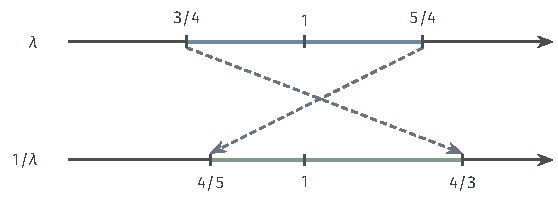
\includegraphics{figures/03-graphs/05-matrices-and-spectra/tikz/sparsification-inverse-band/figure.pdf}
  \caption{能量坐标中谱值的允许区间。虚线示意两端取倒数后怎样换位：靠左的$1-\varepsilon$变到$1/(1-\varepsilon)$一端。中间的$1$保持不动。}
  \label{fig:sparsification-inverse-band}
\end{BookInlineFigure}

将三个因子依次反向取逆，$\bm A^{-1}=\bm L_G^{1/2}\bm L_H^{-1}\bm L_G^{1/2}$。对逆矩阵的比较式两边同乘$\bm L_G^{-1/2}$，中间还原为$\bm L_H^{-1}$，上下界的单位阵还原为$\bm L_G^{-1}$。在全体向量上，两个逆都在常数方向取零，由此得到伪逆的比较
\begin{equation}
\frac{1}{1+\varepsilon}\bm L_G^\dagger
\preceq \bm L_H^\dagger
\preceq \frac{1}{1-\varepsilon}\bm L_G^\dagger.
\label{eq:graph-sparsification-inverse-order}
\end{equation}

把两点差向量$\bm e_u-\bm e_v$代入这三个二次型。按第~\ref{sec:graph-effective-resistance}节的有效电阻公式，
\begin{equation}
\frac{R_G(u,v)}{1+\varepsilon}
\leq R_H(u,v)
\leq \frac{R_G(u,v)}{1-\varepsilon}.
\label{eq:graph-sparsification-resistance}
\end{equation}
直觉上，替代图若整体提高了能量，通相同电流所需的电势差会降低——这对应了取逆之后比例关系的翻转。

\paragraph{方程解的保持}

设$\bm b\in\bm 1^\perp$，$\bm x_G=\bm L_G^\dagger\bm b$是原图的零均值解，$\bm x_H=\bm L_H^\dagger\bm b$是替代图的零均值解。我们想知道用$\bm x_H$代替$\bm x_G$会产生多大的误差。

先把两个解都放到原图的能量坐标中。令$\bm y_G=\bm L_G^{1/2}\bm x_G$，$\bm y_H=\bm L_G^{1/2}\bm x_H$。在这个坐标下，原解变成了
\[
\bm y_G=\bm L_G^{-1/2}\bm b.
\]
把$\bm x_H=\bm L_G^{-1/2}\bm y_H$代入替代图的方程$\bm L_H\bm x_H=\bm b$，两边左乘$\bm L_G^{-1/2}$，得到
\[
\bm A\bm y_H=\bm L_G^{-1/2}\bm b.
\]
右端和原解的方程相同，因此$\bm y_H=\bm A^{-1}\bm y_G$。两解的差为
\[
\bm y_H-\bm y_G=(\bm A^{-1}-\bm I)\bm y_G.
\]
在$\bm A$的正交特征基中，$\bm A^{-1}-\bm I$把每个方向乘以$1/\lambda-1$，其中$\lambda$是该方向的特征值。因为$1-\varepsilon\leq\lambda\leq1+\varepsilon$，这个乘数的绝对值至多是$\varepsilon/(1-\varepsilon)$。

按坐标定义，新坐标中的普通长度就是原图能量的平方根。因此
\begin{equation}
\lVert\bm x_H-\bm x_G\rVert_{\bm L_G}
\leq \frac{\varepsilon}{1-\varepsilon}
      \lVert\bm x_G\rVert_{\bm L_G},
\label{eq:graph-sparsification-solution-error}
\end{equation}
其中$\lVert\bm z\rVert_{\bm L_G}=\sqrt{\bm z^\top\bm L_G\bm z}$是$\bm 1^\perp$上的能量范数。这个界控制的是误差在原图上的总沿边变化，而非某个特定坐标的相对误差——如果某个坐标恰好为零，无法以它为分母给出相对界。

用于电阻查询时应读式~\eqref{eq:graph-sparsification-resistance}，用于方程近似时应读式~\eqref{eq:graph-sparsification-solution-error}，只评估划分目标时割权和体积的比较已经足够。

\section{稀疏图的构造}
\label{sec:graph-resistance-sampling}

明确了谱近似的目标后，接下来的核心问题是：\emph{如何从原图$\mathcal G$的$m$条边中只选出少量的边，构造出满足$(1-\varepsilon)\bm L_G\preceq\bm L_H\preceq(1+\varepsilon)\bm L_G$的稀疏图$\mathcal H$？}Spielman与Srivastava于2011年给出了一种随机抽样构造法：以每条边的电导与有效电阻之积$c_e R_e$作为重要性权重，从原图边集中独立有放回地抽取$q$次边，并对抽中的边按概率倒数补偿权重\scite{spielman2011graph}。本节分三步介绍抽样分布的选择、具体算法实现以及基于矩阵Chernoff界的理论证明。

\subsection{抽样分布的选择}
\label{sec:graph-resistance-sampling-distribution}

要通过随机抽边构造稀疏图，首先需要决定每条边$e\in E$在单次抽取中被选中的概率$p_e$。最朴素的想法是所有边等概率抽取（$p_e=1/m$），但它可能以很高概率漏掉维持连通性的桥边。

\paragraph{均匀抽样的风险}

考察图~\ref{fig:graph-sparsification-bridge}所示的杠铃图：左右两个稠密大团之间只有一条唯一的桥边$e_{\mathrm{bridge}}$。若在全部$m$条边中等概率独立抽样$q$次（$q\ll m$），则单次未抽中桥边的概率为$1-1/m$，连续$q$次都漏掉桥边的概率高达$(1-1/m)^q\approx\mathrm e^{-q/m}\approx 1$。

漏掉桥边会使谱近似下界不成立。为说明这一点，取一个在左团所有顶点上赋$1$、在右团所有顶点上赋$0$的测试向量$\bm x$。在左右两个团内部，每条边两端取值相同，能量贡献全为$0$；整张图在$\bm x$方向上的非零能量$\bm x^\top\bm L_G\bm x=c_{e_{\mathrm{bridge}}}>0$完全由这条桥边独自承担。漏掉桥边会使替代图在该方向上的能量变为$\bm x^\top\bm L_H\bm x=0$，直接违背谱近似要求的正下界$(1-\varepsilon)\bm x^\top\bm L_G\bm x$。

\begin{figure}[!htb]
  \centering
  \begingroup
\definecolor{SparseBridgeBlue}{HTML}{7188A3}
\definecolor{SparseBridgeBlueFill}{HTML}{E5EAF0}
\definecolor{SparseBridgeYellow}{HTML}{B4A16F}
\definecolor{SparseBridgeNeutral}{HTML}{4C4D4F}
\definecolor{SparseBridgeText}{HTML}{3B4252}
\begin{tikzpicture}[x=10mm,y=10mm,
  vertex/.style={circle,draw=SparseBridgeBlue,fill=SparseBridgeBlueFill,
    minimum size=3.2mm,inner sep=0pt,line width=.65pt},
  inneredge/.style={draw=SparseBridgeNeutral,line width=.75pt},
  bridge/.style={draw=SparseBridgeYellow,line width=1.4pt},
  text=SparseBridgeText]
  \coordinate (l1) at (0,0);
  \coordinate (l2) at (.75,.65);
  \coordinate (l3) at (1.5,0);
  \coordinate (l4) at (.75,-.65);
  \coordinate (r1) at (3.5,0);
  \coordinate (r2) at (4.25,.65);
  \coordinate (r3) at (5,0);
  \coordinate (r4) at (4.25,-.65);
  \draw[inneredge] (l1) -- (l2) -- (l3) -- (l4) -- cycle
                    (l1) -- (l3) (l2) -- (l4);
  \draw[inneredge] (r1) -- (r2) -- (r3) -- (r4) -- cycle
                    (r1) -- (r3) (r2) -- (r4);
  \draw[bridge] (l3) -- node[above,font=\footnotesize\sffamily]{桥} (r1);
  \foreach \point in {l1,l2,l3,l4,r1,r2,r3,r4}{
    \node[vertex] at (\point) {};
  }
  \node[below,font=\footnotesize] at (.75,-.87) {$x_v=1$};
  \node[below,font=\footnotesize] at (4.25,-.87) {$x_v=0$};
\end{tikzpicture}
\endgroup

  \caption{两个稠密团之间仅靠一条桥边相连。取在左团恒为$1$、右团恒为$0$的顶点函数时，两团内部边毫无能量贡献，桥边独自承担该方向的全部能量；若抽样漏掉桥边，谱近似立刻失效。}
  \label{fig:graph-sparsification-bridge}
\end{figure}

\paragraph{按有效电阻分配抽样概率}

怎样自动识别出像桥边这样决定某些方向上全部能量的边？第~\ref{sec:graph-sparsification-resistance-trees}小节建立的有效电阻与生成树理论已经给出了答案。一方面，由定理~\ref{thm:graph-tree-edge-probability}，每条边$e$的电导与有效电阻之积$c_e R_e\in(0,1]$恰好等于该边出现在随机生成树中的概率$\mathbb P(e\in T)=c_e R_e$：对于唯一的桥边，$c_e R_e=1$；而对于存在大量并联替代路径的稠密团内边，$c_e R_e$很小（如$K_n$中仅为$2/n$）。另一方面，由Foster定理（定理~\ref{thm:graph-foster-theorem}），在含$n$个顶点的连通图上，全体边的$c_e R_e$之和恒等于常数$\sum_{e\in E}c_e R_e=n-1$。

因此，将每条边的$c_e R_e$除以归一化常数$n-1$，就得到了一个合法的边抽样概率分布：
\begin{equation}
p_e=\frac{c_eR_e}{\sum_{f\in E}c_fR_f}=\frac{c_eR_e}{n-1}\qquad(e\in E).
\label{eq:graph-resistance-sampling-probability}
\end{equation}
在连通正权图（$n\geq 2$）上，每条正权边的有效电阻$R_e>0$，故$p_e>0$且$\sum_{e\in E}p_e=1$。

\paragraph{重加权补偿与单次波动界}

有了抽样概率$\{p_e\}_{e\in E}$，我们从边集中按分布$p_e$独立有放回地抽取$q$次，记第$j$次抽中的边为$e_j$（$j=1,\ldots,q$）。对于任意一条固定边$e\in E$，它在单次抽取中被选中的概率是$p_e$，$q$次抽取中平均被选中$qp_e$次。为了让它在替代图$\mathcal H$中的\emph{期望总权重}恰好等于原图权重$c_e$，规定每当边$e$被抽中一次，就给它的新权重累加$\frac{c_e}{qp_e}$（抽中概率$p_e$越小的边，一旦抽中获得的单次权重补偿越大）。将全部$q$次抽取的秩一拉普拉斯项相加，得到稀疏图$\mathcal H$的拉普拉斯矩阵：
\begin{equation}
\bm L_H
=\sum_{j=1}^q \frac{c_{e_j}}{qp_{e_j}}
     \bm b_{e_j}\bm b_{e_j}^\top.
\label{eq:graph-resistance-sampling-laplacian}
\end{equation}
沿用式~\eqref{eq:graph-sparsification-normalized-order}在正交补空间$\bm 1^\perp$上的原图能量坐标$\bm y=\bm L_G^{1/2}\bm x$，将第$j$次抽中边$e_j$所贡献的标准化秩一随机矩阵记为
\begin{equation}
\bm X_j=\frac{c_{e_j}}{qp_{e_j}}
     (\bm L_G^{-1/2}\bm b_{e_j})
     (\bm L_G^{-1/2}\bm b_{e_j})^\top.
\label{eq:graph-resistance-sampling-standardized}
\end{equation}
下面的引理揭示了有效电阻抽样分布$p_e=\frac{c_e R_e}{n-1}$如下代数性质：它不仅保证了期望无偏（$\mathbb E[\bm L_H]=\bm L_G$），而且把每一条边在最坏能量方向上的单次算子范数$\lVert\bm X_j\rVert_2$完全拉平为同一个常数$\frac{n-1}{q}$。

\begin{lemma}[有效电阻抽样的无偏性与单次范数界]
\label{lem:graph-resistance-sampling-moments}
设连通正权图按概率$p_e=c_eR_e/(n-1)$独立有放回抽取$q$次边构造式~\eqref{eq:graph-resistance-sampling-laplacian}的$\bm L_H$。则：
\begin{enumerate}
  \item 抽样矩阵的期望等于原图拉普拉斯矩阵：
  \begin{equation}
  \mathbb E[\bm L_H]=\bm L_G,\qquad
  \mathbb E\!\left[\sum_{j=1}^q\bm X_j\right]=\bm I_{\bm 1^\perp}.
  \label{eq:graph-resistance-sampling-expectation}
  \end{equation}
  \item 不论第$j$次抽中哪一条边$e_j\in E$，标准化单次矩阵$\bm X_j$都是对称半正定的，且其算子谱范数恒等于
  \[
    \lVert\bm X_j\rVert_2=\frac{n-1}{q}.
  \]
\end{enumerate}
\end{lemma}

\begin{proof}
（1）对固定的第$j$次抽样，随机矩阵$\bm Y_j=\frac{c_{e_j}}{qp_{e_j}}\bm b_{e_j}\bm b_{e_j}^\top$以概率$p_e$取值为$\frac{c_e}{qp_e}\bm b_e\bm b_e^\top$（$e\in E$）。因此单次期望为
\[
  \mathbb E[\bm Y_j]
  =\sum_{e\in E}p_e\cdot\frac{c_e}{qp_e}\bm b_e\bm b_e^\top
  =\frac{1}{q}\sum_{e\in E}c_e\bm b_e\bm b_e^\top
  =\frac{1}{q}\bm L_G.
\]
对$j=1,\ldots,q$求和即得$\mathbb E[\bm L_H]=\bm L_G$；两侧在$\bm 1^\perp$上夹乘$\bm L_G^{-1/2}$即得$\mathbb E\bigl[\sum_{j=1}^q\bm X_j\bigr]=\bm L_G^{-1/2}\bm L_G\bm L_G^{-1/2}=\bm I_{\bm 1^\perp}$。

（2）记向量$\bm v_j=\bm L_G^{-1/2}\bm b_{e_j}\in\bm 1^\perp$，则$\bm X_j=\frac{c_{e_j}}{qp_{e_j}}\bm v_j\bm v_j^\top$是正标量与向量外积的乘积，故对称半正定且秩为$1$，其唯一非零特征值（即算子范数$\lVert\bm X_j\rVert_2$）等于系数乘以$\lVert\bm v_j\rVert_2^2$。注意到$\bm v_j$的欧氏长度平方恰好就是边$e_j$两端的有效电阻：
\[
\lVert\bm v_j\rVert_2^2
=\bm b_{e_j}^\top\bm L_G^\dagger\bm b_{e_j}
=R_{e_j}.
\]
将$p_{e_j}=c_{e_j}R_{e_j}/(n-1)$代入$\lVert\bm X_j\rVert_2=\frac{c_{e_j}}{qp_{e_j}}\lVert\bm v_j\rVert_2^2$，分子与分母中的$c_{e_j}R_{e_j}$精确对消：
\[
\lVert\bm X_j\rVert_2
=\frac{c_{e_j}R_{e_j}}{qp_{e_j}}
=\frac{n-1}{q}.\qedhere
\]
\end{proof}

\subsection{算法实现}
\label{sec:graph-resistance-sampling-algorithm}

将上述抽样与重加权规则整理为如下算法。

\begin{algorithm}[按有效电阻抽样构造稀疏图]
\label{alg:graph-resistance-sampling}
输入：连通正权图$\mathcal G=(V,E,c)$的边表与各边有效电阻$\widehat R_e$（精确值或严格为正且带相对误差保证的估计值），抽样次数$q$。输出：顶点集为$V$的稀疏重加权子图$\mathcal H=(V,E_H,\widehat c)$。
\begin{enumerate}
  \item \textbf{计算抽样分布}：对每条边$e\in E$计算权重积$c_e\widehat R_e$，归一化为概率分布$p_e=c_e\widehat R_e/\sum_{f\in E}c_f\widehat R_f$，建立累计概率表并将所有边的输出权重$\widehat c_e$初始化为$0$。
  \item \textbf{独立有放回抽样与重加权}：独立重复$q$次：在$[0,1)$上生成均匀随机数，按累计概率表定位抽中的边$e$，将其输出权重累加$\widehat c_e\leftarrow\widehat c_e+c_e/(qp_e)$。
  \item \textbf{输出稀疏图}：保留全部原图顶点$V$，输出所有满足$\widehat c_e>0$的边及其累计权重$\widehat c_e$。
\end{enumerate}
\end{algorithm}

在第一步与第二步的实现中，可将区间$[0,1)$按边表顺序切分为$m$个长度分别为$p_{e_1},\ldots,p_{e_m}$的相邻子区间；每次抽取时用二分查找在$O(\log m)$时间内定位随机数落入的子区间（或用Walker别名表在$O(m)$预处理后实现每次$O(1)$时间抽样）。若算出的所需抽样次数$q\geq m$，则直接返回原图$\mathcal G$即可。

\begin{example}[四点五边图上的有效电阻抽样与重加权过程]
\label{ex:graph-resistance-sampling}
在例~\ref{ex:graph-sparsification-trees}的四点五边单位权图上演示算法~\ref{alg:graph-resistance-sampling}。四条环边的$c_e R_e=5/8$，对角边$13$的$c_e R_e=1/2$，Foster总和为$n-1=3$。归一化后得到四条环边的抽样概率均为$p_e=\frac{5/8}{3}=\frac{5}{24}$，对角边$13$的抽样概率为$p_{13}=\frac{1/2}{3}=\frac{1}{6}$。

为展示重加权规则，这里不使用$q\geq m$时返回原图的快捷处理，取演示样本数$q=6$；这一小样本演示本身不声称满足给定谱精度。每当抽中一条环边，其权重累加$\frac{1}{6\times(5/24)}=\frac{4}{5}$；每当抽中对角边$13$，其权重累加$\frac{1}{6\times(1/6)}=1$（对角边抽中概率较小，单次补偿权重更高）。

假设$6$次随机数依次抽中边$12,23,34,41,13,12$（图~\ref{fig:sparsification-sampling-intervals}标出了第$1$次和第$6$次随机数均落入边$12$的概率区间），表~\ref{tab:graph-resistance-sampling}记录了各步权重的累加过程。最终边$12$因被抽中两次而获得权重$\frac85$，其余三条环边权重为$\frac45$，对角边权重为$1$。
\end{example}

\begin{BookInlineFigure}
  \centering
  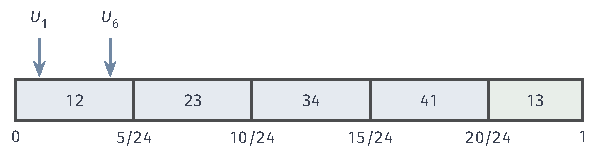
\includegraphics{figures/03-graphs/05-matrices-and-spectra/tikz/sparsification-sampling-intervals/figure.pdf}
  \caption{按各边抽样概率$p_e$切分单位区间$[0,1)$。区间内的两位数字表示边的端点。第$1$次和第$6$次的均匀随机数都落入边$12$的区间$[0,5/24)$内，因此两次增量$\frac45$均累加在边$12$上。}
  \label{fig:sparsification-sampling-intervals}
\end{BookInlineFigure}

\begin{table}[!htb]
  \centering
  \caption{四点五边图在$q=6$次抽样下的边权累加过程。}
  \label{tab:graph-resistance-sampling}
  \begin{tabular}{ccrrrrr}
    \toprule
    抽样序号 & 抽中的边 & $\widehat c_{12}$ & $\widehat c_{23}$ & $\widehat c_{34}$ & $\widehat c_{41}$ & $\widehat c_{13}$ \\
    \midrule
    1 & $12$ & $4/5$ & 0 & 0 & 0 & 0 \\
    2 & $23$ & $4/5$ & $4/5$ & 0 & 0 & 0 \\
    3 & $34$ & $4/5$ & $4/5$ & $4/5$ & 0 & 0 \\
    4 & $41$ & $4/5$ & $4/5$ & $4/5$ & $4/5$ & 0 \\
    5 & $13$ & $4/5$ & $4/5$ & $4/5$ & $4/5$ & 1 \\
    6 & $12$ & $8/5$ & $4/5$ & $4/5$ & $4/5$ & 1 \\
    \bottomrule
  \end{tabular}
\end{table}

\subsection{算法分析}
\label{sec:graph-resistance-sampling-analysis}

引理~\ref{lem:graph-resistance-sampling-moments}(1)保证了抽样图在平均意义下满足$\mathbb E[\bm L_H]=\bm L_G$；但实际算法只生成一张随机图$\mathcal H$，我们需要保证这张图以高概率\emph{同时在所有向量方向$\bm x\in\mathbb R^n$上}满足$(1-\varepsilon)\bm x^\top\bm L_G\bm x\leq\bm x^\top\bm L_H\bm x\leq(1+\varepsilon)\bm x^\top\bm L_G\bm x$。

在正交补空间$\bm 1^\perp$的能量坐标下，所有方向上的二次型能量比值都被夹在随机矩阵和$\sum_{j=1}^q\bm X_j$的最小特征值与最大特征值之间。因此，全部方向同时满足$1\pm\varepsilon$谱近似，当且仅当算子范数偏差满足$\bigl\lVert\sum_{j=1}^q\bm X_j-\bm I_{\bm 1^\perp}\bigr\rVert_2\leq\varepsilon$。下面的\term{矩阵Chernoff界}（matrix Chernoff bound）\scite{tropp2012userfriendly}专门用于控制独立随机半正定矩阵和的极端特征值偏离。

\begin{theorem}[矩阵Chernoff界的单位均值形式]
\label{thm:graph-matrix-chernoff}
设$\bm X_1,\ldots,\bm X_q$是相互独立的$d\times d$随机对称半正定矩阵，满足对每个$j$恒有$\lVert\bm X_j\rVert_2\leq r$，且期望之和为单位矩阵$\sum_{j=1}^q\mathbb E[\bm X_j]=\bm I_d$。则对任意$0<\varepsilon<1$，有
\begin{equation}
\mathbb P\!\left(
  \left\lVert\sum_{j=1}^q\bm X_j-\bm I_d\right\rVert_2>\varepsilon
\right)
\leq 2d\exp\!\left(-\frac{\varepsilon^2}{3r}\right).
\label{eq:graph-matrix-chernoff}
\end{equation}
\end{theorem}

将引理~\ref{lem:graph-resistance-sampling-moments}建立的无偏性与单次范数界$r=(n-1)/q$代入定理~\ref{thm:graph-matrix-chernoff}，立即可导出有效电阻抽样的谱稀疏化主定理。

\begin{theorem}[有效电阻抽样的谱稀疏化保证]
\label{thm:graph-resistance-sparsification}
设$\mathcal G$是含$n\geq 2$个顶点的连通正权图，给定相对误差$0<\varepsilon<1$与失败概率上限$0<\delta<1$。若按有效电阻概率$p_e=c_eR_e/(n-1)$执行算法~\ref{alg:graph-resistance-sampling}，且抽样次数$q$满足
\begin{equation}
q\geq\frac{3(n-1)}{\varepsilon^2}
         \log\frac{2(n-1)}{\delta},
\label{eq:graph-resistance-sampling-count}
\end{equation}
则输出的包含至多$\min\{m,q\}$条边的重加权子图$\mathcal H$以至少$1-\delta$的概率是$\mathcal G$的$\varepsilon$谱近似：
\[
  (1-\varepsilon)\bm L_G\preceq\bm L_H\preceq(1+\varepsilon)\bm L_G.
\]
\end{theorem}

\begin{proof}
在维数$d=n-1$的子空间$\bm 1^\perp$上考察独立随机半正定矩阵$\bm X_1,\ldots,\bm X_q$。由引理~\ref{lem:graph-resistance-sampling-moments}，有$\sum_{j=1}^q\mathbb E[\bm X_j]=\bm I_{\bm 1^\perp}$且$\lVert\bm X_j\rVert_2=(n-1)/q=r$。代入式~\eqref{eq:graph-matrix-chernoff}得
\[
\mathbb P\!\left(
  \left\lVert\sum_{j=1}^q\bm X_j-\bm I_{\bm 1^\perp}\right\rVert_2>\varepsilon
\right)
\leq 2(n-1)\exp\!\left(-\frac{q\varepsilon^2}{3(n-1)}\right).
\]
当$q$满足式~\eqref{eq:graph-resistance-sampling-count}时，右端失败概率不超过$\delta$。在概率至少为$1-\delta$的成功事件上，对任意$\bm y=\bm L_G^{1/2}\bm x\in\bm 1^\perp$都有$(1-\varepsilon)\lVert\bm y\rVert_2^2\leq\bm y^\top\bigl(\sum_{j=1}^q\bm X_j\bigr)\bm y\leq(1+\varepsilon)\lVert\bm y\rVert_2^2$，换回原坐标即得$(1-\varepsilon)\bm x^\top\bm L_G\bm x\leq\bm x^\top\bm L_H\bm x\leq(1+\varepsilon)\bm x^\top\bm L_G\bm x$。又因常向量$\bm 1$在$\bm L_G$与$\bm L_H$下的二次型均为$0$，该不等式对全体$\bm x\in\mathbb R^n$成立。
\end{proof}

若算法~\ref{alg:graph-resistance-sampling}使用的是第~\ref{sec:electrical-approximate-resistance}小节求得的近似有效电阻$\widehat R_e\in[(1-\eta)R_e,(1+\eta)R_e]$（$0\leq\eta<1$），则实际抽样概率满足$\widehat p_e\geq\frac{1-\eta}{1+\eta}p_e$，单次范数上界至多放大为$r=\frac{1+\eta}{1-\eta}\cdot\frac{n-1}{q}$。因此，将式~\eqref{eq:graph-resistance-sampling-count}中的抽样次数乘以$(1+\eta)/(1-\eta)$即可控制条件于电阻估计成功事件的抽样失败概率。当$\eta$固定且远离$1$时，这才是常数因子；若估计本身以概率至多$\delta_R$失败，则总失败概率至多为$\delta_R+\delta$。

边数为$O(n\log(n/\delta)/\varepsilon^2)$并不单独证明构造时间近线性：总成本还包含有效电阻估计、概率表预处理和抽样。采用相应的快速拉普拉斯求解器并控制求解误差，才能得到近线性的构造时间保证。

\section{稀疏图作为预条件}
\label{sec:graph-sparse-preconditioning}

拿到一张谱近似图之后，一个直接的用途是帮助求解原图上的拉普拉斯方程$\bm L_G\bm x=\bm b$。

求解的基本循环是这样的。给定当前的猜测$\bm x$，先算出它在原图上还差多少——残差$\bm r=\bm b-\bm L_G\bm x$。如果能精确解一次$\bm L_G\bm z=\bm r$，那么把$\bm z$加到$\bm x$上就直接补齐了差额。但这需要再解一次原图方程，和原问题一样难。

换一个思路：用边数少得多的近似图$\mathcal H$来求方向。也就是解$\bm L_H\bm z=\bm r$，把$\bm z$作为修正方向。这个方向不完全正确，因为$\bm L_H$和$\bm L_G$不一样。但如果两者足够接近，方向偏差不大，沿着它调整后再回到原图检查残差，几轮下来就能逼近真解。每轮用原图算残差确保终点准确，用稀疏图算方向减少计算量——这就是预条件的思路。

设原图$\mathcal G$连通，相容右端$\bm b\in\bm 1^\perp$，取$\mathcal G$的一个$\varepsilon$谱近似图$\mathcal H$（$0<\varepsilon<1$），以其拉普拉斯矩阵$\bm M=\bm L_H$作为预条件矩阵。在正交补空间$\bm 1^\perp$上，$\bm L_G$与$\bm M$均对称正定。下面的定理给出预条件算子的条件数上界以及\term{预条件共轭梯度法}（preconditioned conjugate gradient method，PCG）的收敛速度。

\begin{theorem}[谱近似预条件的条件数与收敛界]
\label{prop:graph-sparse-preconditioner}
设连通图$\mathcal G$的替代图$\mathcal H$满足$(1-\varepsilon)\bm L_G\preceq\bm M=\bm L_H\preceq(1+\varepsilon)\bm L_G$（$0<\varepsilon<1$）。在$\bm 1^\perp$上定义对称正定预条件算子$\bm A=\bm M^{-1/2}\bm L_G\bm M^{-1/2}$，则：
\begin{enumerate}
  \item 广义Rayleigh商与预条件算子$\bm A$的谱条件数满足
  \begin{equation}
  \frac{1}{1+\varepsilon}
  \leq
  \frac{\bm x^\top\bm L_G\bm x}{\bm x^\top\bm M\bm x}
  \leq
  \frac{1}{1-\varepsilon}\quad(\forall\bm x\in\bm 1^\perp\setminus\{\bm 0\}),
  \qquad
  \kappa_2(\bm A)\leq\frac{1+\varepsilon}{1-\varepsilon}.
  \label{eq:graph-sparse-preconditioned-condition}
  \end{equation}
  \item 以$\bm M$为预条件矩阵求解$\bm L_G\bm x=\bm b$（$\bm b\in\bm 1^\perp$，记零均值精确解为$\bm x_*=\bm L_G^\dagger\bm b$），预条件共轭梯度法第$k$步迭代解$\bm x^{(k)}$满足
  \begin{equation}
  \lVert\bm x^{(k)}-\bm x_*\rVert_{\bm L_G}
  \leq
  2\left(\frac{\sqrt\kappa-1}{\sqrt\kappa+1}\right)^k
  \lVert\bm x^{(0)}-\bm x_*\rVert_{\bm L_G},
  \qquad \kappa=\kappa_2(\bm A)\leq\frac{1+\varepsilon}{1-\varepsilon}.
  \label{eq:graph-sparse-preconditioned-cg-error}
  \end{equation}
\end{enumerate}
\end{theorem}

\begin{proof}
（1）对任意非零$\bm x\in\bm 1^\perp$，将$(1-\varepsilon)\bm x^\top\bm L_G\bm x\leq\bm x^\top\bm M\bm x\leq(1+\varepsilon)\bm x^\top\bm L_G\bm x$移项取倒数，即得广义Rayleigh商夹逼式：
\begin{equation}
\frac{1}{1+\varepsilon}
\leq
\frac{\bm x^\top\bm L_G\bm x}{\bm x^\top\bm M\bm x}
\leq
\frac{1}{1-\varepsilon}.
\label{eq:graph-sparse-preconditioned-rayleigh}
\end{equation}
作可逆坐标变换$\bm y=\bm M^{1/2}\bm x\in\bm 1^\perp$，则$\frac{\bm x^\top\bm L_G\bm x}{\bm x^\top\bm M\bm x}=\frac{\bm y^\top\bm A\bm y}{\bm y^\top\bm y}$正是$\bm A=\bm M^{-1/2}\bm L_G\bm M^{-1/2}$的普通Rayleigh商。因此$\lambda_{\min}(\bm A)\geq\frac{1}{1+\varepsilon}$且$\lambda_{\max}(\bm A)\leq\frac{1}{1-\varepsilon}$，两者相除即得$\kappa_2(\bm A)=\frac{\lambda_{\max}(\bm A)}{\lambda_{\min}(\bm A)}\leq\frac{1+\varepsilon}{1-\varepsilon}$。

（2）将$\bm x=\bm M^{-1/2}\bm y$代入$\bm L_G\bm x=\bm b$并左乘$\bm M^{-1/2}$，转化为等价的对称正定系统$\bm A\bm y=\bm M^{-1/2}\bm b$（精确解为$\bm y_*=\bm M^{1/2}\bm x_*$）。对任意向量$\bm e=\bm x-\bm x_*$，对应变换后误差$\bm d=\bm y-\bm y_*=\bm M^{1/2}\bm e$的$\bm A$-能量范数平方恰好等于$\bm e$的原图$\bm L_G$-能量范数平方：
\[
  \lVert\bm d\rVert_{\bm A}^2=\bm d^\top\bm A\bm d=(\bm M^{1/2}\bm e)^\top\bm M^{-1/2}\bm L_G\bm M^{-1/2}(\bm M^{1/2}\bm e)=\bm e^\top\bm L_G\bm e=\lVert\bm e\rVert_{\bm L_G}^2.
\]
直接对$\bm A\bm y=\bm M^{-1/2}\bm b$应用第~\ref{sec:electrical-numerical-solve}小节的共轭梯度误差界~\eqref{eq:electrical-cg-error}，即得式~\eqref{eq:graph-sparse-preconditioned-cg-error}。
\end{proof}

在实际执行预条件共轭梯度法时，无需显式计算平方根$\bm M^{1/2}$，而是在原坐标下每轮只做两项核心操作：先在原图$\mathcal G$上计算一次矩阵向量乘法$\bm L_G\bm p$以更新步长与残差$\bm r$，再在稀疏图$\mathcal H$上求解一次预条件方程$\bm M\bm z=\bm r$以获得修正方向$\bm z$（完整算法递推见\BookChapterRef{chap:krylov-methods}{卷二“Krylov子空间法”章}）。

若采用单点接地方式，只需在$\mathcal G$和$\mathcal H$中选取同一个接地点$q$：将接地点坐标取零的向量代入式~\eqref{eq:graph-spectral-approximation-energy}，即知两个$(n-1)\times(n-1)$约化正定矩阵$\overline{\bm L}_G$与$\overline{\bm M}=\overline{\bm L}_H$满足完全相同的谱近似界和条件数上界~\eqref{eq:graph-sparse-preconditioned-condition}。

\paragraph{一个完整的迭代例子}

用四点五边图直接看预条件后的效果。令$\mathcal G$为单位权五边图，$\mathcal H$删去对角线$13$后只保留单位权四环。两图在$\bm 1^\perp$上有三个独立的零和方向。

先看$\bm u=(1,0,-1,0)^\top$。对角边两端之差为$2$，贡献能量$4$，加上四条环边各$1$，原图能量为$8$。四环没有对角边，能量只有$4$。广义Rayleigh商$8/4=2$。

再看与$\bm u$正交的零和方向，比如$\bm v=(0,1,0,-1)^\top$。此时对角边两端同值$0$，不贡献能量。两图能量都是$4$（该向量长度平方为$2$、特征值为$2$），商为$1$。

还有一个方向（如$(1,-1,1,-1)^\top/2$归一化），也可核对对角边上差为零。因此四环$\bm M$在$\bm u$方向的特征值是$2$，添对角边后$\bm L_G$在同方向变为$4$，而其余两个方向上两图一样。预条件矩阵$\bm A$的三个特征值为$1,1,2$。通用界$\varepsilon=1/2$给出条件数上界$(1+1/2)/(1-1/2)=3$，覆盖了实际条件数$2$。

用同一例子走一轮迭代。设右端$\bm b=\bm u+\bm v$，初值为零。第一次残差就是$\bm b$。在四环上解$\bm M\bm z=\bm b$，得到$\bm z=(\bm u+\bm v)/2$。

沿$\bm z$更新时，步长由原图决定。因为$\bm u,\bm v$正交且长度平方都是$2$，
\[
\bm b^\top\bm z=2,
\qquad
\bm z^\top\bm L_G\bm z=3.
\]
步长为$2/3$。更新后$\bm x^{(1)}=(\bm u+\bm v)/3$。残差为
\[
\bm b-\bm L_G\bm x^{(1)}
=\frac{-\bm u+\bm v}{3}.
\]
这个残差还含两个方向，下一轮用它继续修正。图~\ref{fig:sparsification-preconditioner-step}把两张图的分工画了出来：四环给出修正方向，原图决定步长和检验残差。

\begin{BookInlineFigure}
  \centering
  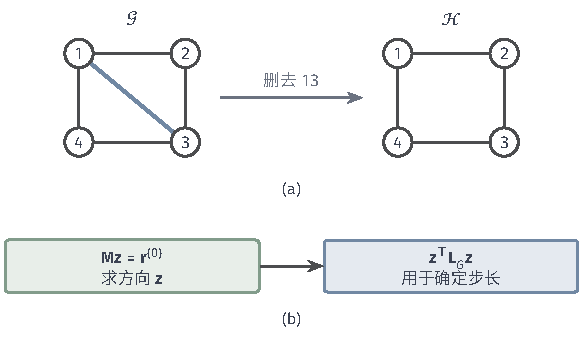
\includegraphics{figures/03-graphs/05-matrices-and-spectra/tikz/sparsification-preconditioner-step/figure.pdf}
  \caption{四点五边图的预条件迭代。（a）原图$\mathcal G$和删去对角边后的四环$\mathcal H$。（b）第一轮用$\mathcal H$的拉普拉斯求方向，用$\mathcal G$的拉普拉斯计算步长和残差。}
  \label{fig:sparsification-preconditioner-step}
\end{BookInlineFigure}

\paragraph{实际代价}

总代价包含三部分：构造稀疏图并准备它的求解器（一次性），每轮在原图上做一次矩阵乘向量（$O(m+n)$），以及每轮在稀疏图上解方程。同一图有多个右端时，可以共享近似图及其分解，把准备成本分摊给多次求解。

稀疏图虽然边少，但直接分解时仍可能产生填充——是否值得要同时比较每轮代价和所需迭代次数。若每轮在近似图上只做有限次内迭代而非精确求解，需要另行控制求解误差，不能直接套用式~\eqref{eq:graph-sparse-preconditioned-cg-error}中精确预条件的结论。

\section{本章小结}
\label{sec:graph-sparsification-summary}

本章研究如何用边数少得多的带权图代替原图，同时近似保持计算结果。

若替代图只用于评价分组，只需保持割权——单点割给出加权度，加权度相加给出体积，割权与体积共同决定导通率和NCut。若还要求特征值、有效电阻或方程解，就需要保持所有实值顶点赋值上的能量，即谱近似。同一个三角形的例子说明，割近似不自动蕴含谱近似：边权的增减可能集中在差异大或差异小的方向上，只看跨边总权无法发现。

每条边在随机生成树中出现的概率是$c_eR_e$，这个乘积由电导和有效电阻共同决定。桥必定出现在每棵树中，团内边只出现在一部分树中。把这些概率除以Foster总和$n-1$，得到加起来等于一的抽样分布。每次抽到一条边后按概率的倒数补偿权重，使平均矩阵恰好等于原矩阵。有效电阻抽样的关键性质是：不论抽到哪条边，单次贡献在标准化坐标中的范数都是同一个值$(n-1)/q$，它均衡了所有边在最坏方向上的波动。矩阵Chernoff界把这个单次上界转为"所有方向同时满足误差"的概率保证。

用稀疏图作预条件时，每轮在原图上算残差，在稀疏图上根据残差求修正方向。两图能量之比越接近一，换坐标后的矩阵越接近恒等算子，条件数越小，所需迭代次数越少。实际节省多少工作，还要加上构造稀疏图和准备其求解器的开销。


\chapter{图上的行走}
\label{chap:graph-walks}

在图的一个顶点放下一枚棋子。每到一处，棋子按邻边的权重比例随机选一个邻居移过去。重复同样的试验——每次从同一个顶点出发，都走五步——统计五步后落在各点的比例，就能估计第五步的位置分布。

位置分布并不是唯一值得关心的问题。另一种问题是：首次到达某个指定顶点需要几步？还有一种更强的问题：把所有顶点都走到需要几步？它们固定的不是步数，而是停止条件，每次试验的步数都可能不同。

对于位置分布，一步选择写成矩阵乘法，多步演化由矩阵的幂给出。归一化拉普拉斯的谱可以判断分布是否最终收敛到平稳状态，并估计达到给定精度需要走多少步。对于等待时间，给目标顶点固定边界值后，首达期望满足接地拉普拉斯方程。往返等待时间还可以直接用有效电阻表示。

最后两节在有向图上加入重启。重启分布给出了行走中断后从哪里重新出发的偏好，由此得到PageRank排名。将重启集中在少数种子上，可以逐点推送尚未处理的概率质量，只访问种子附近的顶点。

除有向排名一节另作说明外，本章取正权支撑连通、至少有两个顶点的有限无向图。记$V$为顶点集，$n=|V|$为顶点数。顶点$i$的加权度为$d_i$，度向量为$\bm{d}=(d_1,\ldots,d_n)^\top$，度矩阵为$\bm{D}=\operatorname{diag}(d_1,\ldots,d_n)$。总加权度$\operatorname{vol}(V)=\sum_{i\in V}d_i$也叫全图的体积。概率分布写成行向量，顶点函数写成列向量。PageRank中的$\alpha\in(0,1)$始终表示重启概率，沿图转移的概率为$1-\alpha$。

\section{随机游走}
\label{sec:graph-random-walk}

一步怎样选邻居，决定了多步以后棋子可能落在哪里。我们先从四点路径上的具体走步出发，明确一步选择的规则，再将所有可能行走的终点汇总为位置分布。

\subsection{随机游走}
\label{sec:graph-walk-rule}

在单位权路径$1\!-\!2\!-\!3\!-\!4$上，把棋子放在顶点$1$。顶点$1$只有一条边连到$2$，所以第一步别无选择，必须走到$2$。

到了$2$之后，面前有两条边：一条回到$1$，一条通往$3$。两条边的权重都是$1$，总共$2$。回到$1$的概率是$1/2$，走到$3$的概率也是$1/2$。如果把从$2$到$3$的边权提高为$3$，那么从$2$离开时两条边的权重共为$1+3=4$，回到$1$的概率变成$1/4$，走到$3$的概率变成$3/4$。选择概率始终由出发顶点的邻边权重决定。

\begin{definition}[随机游走]
\label{def:graph-random-walk}
记$X_t$为第$t$步所在的顶点。给定$X_t=i$，下一步选择$j$的概率与边权$w_{i,j}$成正比，
\begin{equation}
\mathbb{P}(X_{t+1}=j\mid X_0,\ldots,X_t)=\frac{w_{i,j}}{d_i}.
\label{eq:graph-walk-transition-rule}
\end{equation}
若$d_i=0$（孤立顶点），约定棋子停留在原地。
\end{definition}

这条\term{随机游走}（random walk）规则只读取当前位置。即使两次走到$i$的路线完全不同，从$i$出发的下一步概率仍然一样。

用$\nu_i^{(t)}=\mathbb{P}(X_t=i)$记第$t$步在顶点$i$的概率，把各点的概率排成一行，记作$\bm{\nu}^{(t)}$。下标$i$指定顶点，上标$(t)$指定时刻。$\bm{\nu}^{(0)}$就是起点分布。

一条给定的行走序列$v_0,v_1,\ldots,v_k$要求棋子先出现在$v_0$，再依次完成各步转移。每接上一步，就把此前走完该前缀的概率乘上这一跳的转移概率。因此这条行走的概率为
\begin{equation}
\mathbb{P}(X_0=v_0,\ldots,X_k=v_k)
=\nu^{(0)}_{v_0}\prod_{j=0}^{k-1}\frac{w_{v_j,v_{j+1}}}{d_{v_j}}.
\label{eq:graph-walk-path-probability}
\end{equation}

回到单位权路径。从$1$出发，$1\to2\to1$的概率是$1\cdot(1/2)=1/2$，$1\to2\to3$的概率也是$1\cdot(1/2)=1/2$。两条路径走了相同的步数，但中途经过不同的顶点。若包含孤点，对应因子按停留规则取$1$。

\subsection{多步分布}
\label{sec:graph-walk-distributions}

上面计算了单条路径的概率。如果要问"第$t$步落在顶点$j$的概率是多少"，就需要把所有在第$t$步到达$j$的路径概率加起来。转移矩阵把这个求和变成一次矩阵乘法。

\paragraph{转移矩阵}

把从每个顶点出发的一步选择概率排成一行，再把$n$行叠起来，就得到\term{转移矩阵}（transition matrix）$\bm{P}$。第$i$行记录从$i$出发到各点的概率，第$j$列收集各处走到$j$的概率。设加权邻接矩阵为$\bm{W}=(w_{i,j})$，把$\bm{W}$的第$i$行除以$d_i$，等于在左侧乘$\bm{D}^{-1}$，于是
\begin{equation}
\bm{P}=\bm{D}^{-1}\bm{W}.
\label{eq:graph-walk-transition-matrix}
\end{equation}
矩阵元素非负，每行之和为$1$，即$\bm{P}\bm{1}=\bm{1}$。

\paragraph{一步更新}

要算第$t+1$步到达$j$的概率，可以按上一步所在的位置$i$分类。棋子在第$t$步落在$i$的概率是$\nu_i^{(t)}$，从$i$一步到$j$的概率是$P_{i,j}$。把这两个概率相乘再对所有$i$求和，就得到
\begin{equation}
\nu^{(t+1)}_j=\sum_i \nu^{(t)}_i P_{i,j}.
\label{eq:graph-walk-distribution-entry}
\end{equation}

这个求和就是概率行$\bm{\nu}^{(t)}$右乘$\bm{P}$的第$j$个分量。每多走一步，右边就多乘一个$\bm{P}$，从而
\begin{equation}
\bm{\nu}^{(t+1)}=\bm{\nu}^{(t)}\bm{P},
\qquad
\bm{\nu}^{(t)}=\bm{\nu}^{(0)}\bm{P}^t.
\label{eq:graph-walk-distribution}
\end{equation}
取初始分布为顶点$u$上的点质量，$\bm{P}^t$的第$u$行就是第$t$步的分布。

\paragraph{四点路径的前四步}

在单位权路径$1\!-\!2\!-\!3\!-\!4$上，四个顶点的度分别为$1,2,2,1$。转移矩阵为
\[
\bm{P}=\begin{pmatrix}
0&1&0&0\\
1/2&0&1/2&0\\
0&1/2&0&1/2\\
0&0&1&0
\end{pmatrix}.
\]
从顶点$1$出发，初始行只有第一个分量为$1$。第一次乘$\bm{P}$时，只读取$\bm{P}$的第一行，所以一步后全部质量集中在顶点$2$。

第二次乘$\bm{P}$时读取第二行。顶点$2$的$1/2$概率回到$1$，$1/2$概率走到$3$。第三次乘$\bm{P}$时，分别取$\bm{P}$的第一行和第三行各乘$1/2$再相加。包含初态的计算结果为
\[
\begin{array}{c@{\qquad}c}
t&\bm{\nu}^{(t)}\\
0&(1,0,0,0)\\
1&(0,1,0,0)\\
2&(1/2,0,1/2,0)\\
3&(0,3/4,0,1/4)
\end{array}
\]
图~\ref{fig:graph-walk-path-distribution}把各步连起来。顺着顶点$2$在$t=3$处接到的两条箭头往回看，$3/4$中有$1/2$来自顶点$1$（经路线$1\to2$），另有$1/4$来自顶点$3$（经路线$3\to2$）。

图~\ref{fig:graph-walk-bar-chart}以柱状图展示同一组分布。每个面板对应一个时刻，柱高是当前在各顶点的概率。观察概率如何从起点逐步向路径的另一端扩散：$t=1$时质量全部集中在$2$，$t=2$时分到$1$和$3$，$t=3$时已传到$4$。

\begin{figure}[!htb]
\centering
\begin{tikzpicture}[x=1mm,y=1mm,
  bar/.style={fill=FigureBlueFill,draw=FigureBlue,line width=.45pt},
  panel/.style={anchor=mid,font=\figurefont\footnotesize},
  vlabel/.style={font=\figurefont\fontsize{7.5}{9}\selectfont,FigureInk,anchor=north},
  plabel/.style={font=\figurefont\fontsize{7}{8.5}\selectfont,FigureInk,anchor=south}]
  \def\barw{4}
  \def\barscale{20}
  \def\gap{3}
  % Panel t=1: (0,1,0,0)
  \begin{scope}[xshift=0mm]
    \draw[FigureStroke,line width=.4pt] (0,0) -- (0,\barscale+2);
    \draw[FigureStroke,line width=.4pt] (0,0) -- (4*\barw+3*\gap+1,0);
    \foreach \i/\v/\p in {0/1/0, 1/2/1, 2/3/0, 3/4/0} {
      \pgfmathsetmacro{\x}{\i*(\barw+\gap)+1}
      \pgfmathsetmacro{\h}{\p*\barscale}
      \ifnum\p>0
        \fill[bar] (\x,0) rectangle +(\barw,\h);
        \node[plabel] at (\x+\barw/2,\h) {$\p$};
      \fi
      \node[vlabel] at (\x+\barw/2,-1) {$\v$};
    }
    \node[panel] at (16,-8) {(a) $t=1$};
  \end{scope}
  % Panel t=2: (1/2,0,1/2,0)
  \begin{scope}[xshift=38mm]
    \draw[FigureStroke,line width=.4pt] (0,0) -- (0,\barscale+2);
    \draw[FigureStroke,line width=.4pt] (0,0) -- (4*\barw+3*\gap+1,0);
    \foreach \i/\v/\p/\plbl in {0/1/0.5/{1/2}, 1/2/0/{}, 2/3/0.5/{1/2}, 3/4/0/{}} {
      \pgfmathsetmacro{\x}{\i*(\barw+\gap)+1}
      \pgfmathsetmacro{\h}{\p*\barscale}
      \pgfmathparse{\p>0?1:0}
      \ifnum\pgfmathresult=1
        \fill[bar] (\x,0) rectangle +(\barw,\h);
        \node[plabel] at (\x+\barw/2,\h) {$\plbl$};
      \fi
      \node[vlabel] at (\x+\barw/2,-1) {$\v$};
    }
    \node[panel] at (16,-8) {(b) $t=2$};
  \end{scope}
  % Panel t=3: (0,3/4,0,1/4)
  \begin{scope}[xshift=76mm]
    \draw[FigureStroke,line width=.4pt] (0,0) -- (0,\barscale+2);
    \draw[FigureStroke,line width=.4pt] (0,0) -- (4*\barw+3*\gap+1,0);
    \foreach \i/\v/\p/\plbl in {0/1/0/{}, 1/2/0.75/{3/4}, 2/3/0/{}, 3/4/0.25/{1/4}} {
      \pgfmathsetmacro{\x}{\i*(\barw+\gap)+1}
      \pgfmathsetmacro{\h}{\p*\barscale}
      \pgfmathparse{\p>0?1:0}
      \ifnum\pgfmathresult=1
        \fill[bar] (\x,0) rectangle +(\barw,\h);
        \node[plabel] at (\x+\barw/2,\h) {$\plbl$};
      \fi
      \node[vlabel] at (\x+\barw/2,-1) {$\v$};
    }
    \node[panel] at (16,-8) {(c) $t=3$};
  \end{scope}
\end{tikzpicture}
\caption{从顶点$1$出发在四点路径上的前三步位置分布。柱高表示当前在各顶点的概率。$t=1$时全部质量在$2$。$t=2$时分成两半回到$1$和前进到$3$。$t=3$时已到达端点$4$，但$3/4$的质量留在$2$。}
\label{fig:graph-walk-bar-chart}
\end{figure}

\begin{BookInlineFigure}
\centering
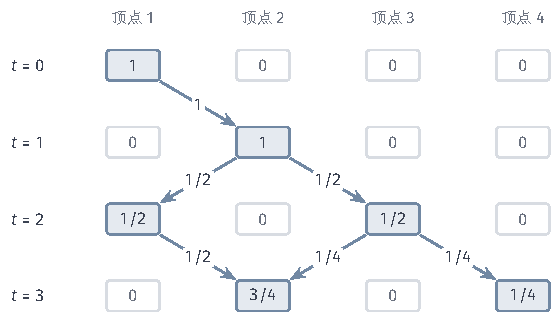
\includegraphics[width=94.132mm]{figures/03-graphs/05-matrices-and-spectra/tikz/walk-examples/path-distribution.pdf}
\caption{单位权路径$1\!-\!2\!-\!3\!-\!4$上从顶点$1$出发的分布。每行对应一个时刻，格内是当前位置的概率，箭头上的数字是这一小股概率在一步中实际转移的量。}
\label{fig:graph-walk-path-distribution}
\end{BookInlineFigure}

\paragraph{与邻接矩阵幂的关系}

第~\ref{chap:graph-adjacency-matrix}章用邻接矩阵$\bm{A}$的幂$(\bm{A}^t)_{u,v}$来计算从$u$到$v$的$t$步行走条数。在无权$d$正则图上，每个顶点的度都是$d$，每一步沿指定边行走的概率为$1/d$。同一条$t$步行走的概率为$d^{-t}$，因此
\[
\bm{P}^t=d^{-t}\bm{A}^t.
\]
度随顶点变化时，同样长的行走可有不同概率，上式不再成立。例如在四点路径上，从顶点$2$出发，$2\to1\to2$的概率是$(1/2)\cdot1=1/2$，$2\to3\to2$的概率是$(1/2)\cdot(1/2)=1/4$。两条路径长度相同，但经过不同度数的顶点，概率不一样。

\section{平稳分布}
\label{sec:graph-walk-stationary}

走了很多步以后，分布会不会停在某个固定形状上？如果给每个顶点分配一定的概率质量，使得一步转移后各点的质量恰好不变，这份分布就叫平稳分布。我们先用四点路径的具体算例看到这样的分布确实存在，再回到一般的无向图推导它的形式。

在四点路径上，试着给每条边的每个端点各分出$1/6$的质量。三条边共分出六份，各顶点收到的份数与自身的邻边数一致：端点$1$和$4$各收到一份，中间的$2$和$3$各收到两份。于是初始质量为$(1,2,2,1)/6$。

现在看一步转移。端点$1$的一份质量全部送给$2$。中间顶点$2$有两份质量，一份送给$1$，另一份送给$3$。边$23$和$34$上的情况也是类似的对称交换。图~\ref{fig:graph-walk-stationary-edge-balance}标出了每条边上的两笔对向转移。任取一个顶点，加起来的流入恰好等于加起来的流出。一步之后各点质量都没有变化。

\begin{BookInlineFigure}
\centering
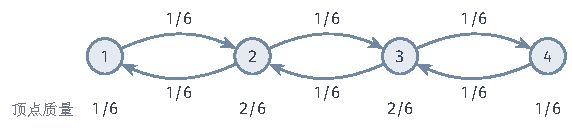
\includegraphics[width=96.936mm]{figures/03-graphs/05-matrices-and-spectra/tikz/walk-examples/stationary-edge-balance.pdf}
\caption{四顶点单位权路径的平稳概率及一步转移量。节点下方是原有质量，同一条边的两个方向各送出$1/6$。}
\label{fig:graph-walk-stationary-edge-balance}
\end{BookInlineFigure}

\begin{definition}[平稳分布]
\label{def:graph-walk-stationary}
若非负行向量$\bm{\pi}$满足$\sum_i\pi_i=1$且
\begin{equation}
\bm{\pi}\bm{P}=\bm{\pi},
\label{eq:graph-walk-stationary}
\end{equation}
则称$\bm{\pi}$是转移矩阵$\bm{P}$的\term{平稳分布}（stationary distribution）。
\end{definition}

上面四点路径的例子提示了一种做法：让每个顶点持有与其度成正比的质量。在一般的加权无向图上，令
\[
\pi_i=\frac{d_i}{\operatorname{vol}(V)}.
\]
下面验证这确实是一个平稳分布。

\paragraph{详细平衡}

考虑一条边$\{i,j\}$上的双向概率流。从$i$送往$j$的流量是当前在$i$的概率乘以从$i$到$j$的转移概率，
\[
\pi_i P_{i,j}=\frac{d_i}{\operatorname{vol}(V)}\cdot\frac{w_{i,j}}{d_i}
=\frac{w_{i,j}}{\operatorname{vol}(V)}.
\]
右边只含边权$w_{i,j}$，与方向无关。交换$i,j$后结果不变，因为$w_{i,j}=w_{j,i}$。这就是说，每条边上从两端送出的概率流相等。这个性质称为\term{详细平衡}（detailed balance）。

既然每条边的双向流已经抵消，对起点$i$求和后，流入$j$的总量自然等于$j$原有的质量$\pi_j$。因此按度分配的分布确实平稳。详细平衡是一个比平稳方程更强的条件：后者只要求每个顶点的总流入等于总流出，前者要求每条边上都各自平衡。

\paragraph{唯一性}

接下来说明连通无向图的平稳分布唯一。

\begin{theorem}[无向连通图的平稳分布]
\label{thm:graph-walk-stationary-uniqueness}
正权支撑连通的有限无向图的转移矩阵$\bm P$有唯一的平稳分布，且$\pi_i=d_i/\operatorname{vol}(V)$。
\end{theorem}

\begin{proof}
设$\bm{q}$是任意一个平稳分布，满足$\bm{q}\bm{P}=\bm{q}$。将等式写成$\bm{q}\bm{D}^{-1}\bm{W}=\bm{q}$，两边转置得
\[
\bm{W}\bm{D}^{-1}\bm{q}^\top=\bm{q}^\top.
\]
这里用了$\bm{W}$对称和$\bm{D}^{-1}$为对角矩阵。

令$\bm{y}=\bm{D}^{-1}\bm{q}^\top$，即$y_i=q_i/d_i$。等式右边的$\bm{q}^\top$可以写成$\bm{D}\bm{y}$，于是
\[
(\bm{D}-\bm{W})\bm{y}=\bm{0}.
\]
左边正是组合拉普拉斯$\bm{L}$作用于$\bm{y}$。第~\ref{chap:graph-laplacian-matrix}章指出，连通图的拉普拉斯零空间由常向量张成。这意味着$y_i=q_i/d_i$对所有$i$取相同的值。由总质量$\sum_i q_i=1$确定这个常数为$1/\operatorname{vol}(V)$，于是
\begin{equation}
\pi_i=\frac{d_i}{\operatorname{vol}(V)}.
\label{eq:graph-walk-stationary-degrees}
\end{equation}
\end{proof}

\paragraph{不连通与收敛的区别}

若图有多个正权连通分量，每个分量可以独立保有自己的概率质量。取各分量平稳分布的任意凸组合仍然平稳，因此唯一性不再成立。孤点上的点质量也可以保留——在停留规则下它已经平稳。

回到只有一条边的两点图。它只有一个正权分量，平稳分布唯一，为$(1/2,1/2)$。但如果从其中一个顶点出发，棋子每一步切换顶点，分布在$(1,0)$与$(0,1)$之间交替，始终不收敛。平稳分布的唯一性回答了"哪些分布保持不变"，至于任意初态能否到达它，还需要检查矩阵幂的行为。

\section{收敛速度}
\label{sec:graph-walk-convergence}

上一节末尾看到，在二部图上单点出发的随机游走会永久奇偶振荡。对于一般的连通无向图，从任意初态$\bm\nu^{(0)}$出发的多步分布$\bm\nu^{(t)}=\bm\nu^{(0)}\bm P^t$究竟何时收敛到平稳分布$\bm\pi$？如果收敛，需要走多少步才能与平稳分布足够接近？本节先将转移矩阵$\bm P$对称化以对接归一化拉普拉斯谱，再导出收敛的充要条件与误差衰减界，最后对比几类典型图的收敛速度。

\subsection{转移矩阵的对称化}
\label{sec:graph-walk-symmetrization}

在度数不均匀的无向图上，虽然边权对称（$w_{i,j}=w_{j,i}$），转移矩阵$\bm P=\bm D^{-1}\bm W$本身通常并\emph{不对称}（例如在四点路径上，$P_{1,2}=1$而$P_{2,1}=1/2$）。为了使用实对称矩阵的正交谱分解，我们对$\bm P$作度平方根相似变换：将第$i$行乘以$\sqrt{d_i}$、第$j$列除以$\sqrt{d_j}$，其$(i,j)$元变为对称的$\frac{w_{i,j}}{\sqrt{d_i d_j}}$。写成矩阵形式，即左乘$\bm D^{1/2}$、右乘$\bm D^{-1/2}$：
\begin{equation}
\bm{S}=\bm{D}^{1/2}\bm{P}\bm{D}^{-1/2}
=\bm{D}^{-1/2}\bm{W}\bm{D}^{-1/2}=\bm{I}-\mathcal{L},
\label{eq:graph-walk-symmetric-transition}
\end{equation}
其中$\mathcal L=\bm D^{-1/2}\bm L\bm D^{-1/2}$正是第~\ref{sec:graph-normalized-laplacian}节的对称归一化拉普拉斯矩阵。

式~\eqref{eq:graph-walk-symmetric-transition}建立起了随机游走与归一化拉普拉斯谱之间的直接桥梁：
\begin{enumerate}
\item \emph{特征值一一对应}：因为$\bm P=\bm D^{-1/2}\bm S\bm D^{1/2}$与实对称矩阵$\bm S$相似，两者的特征值完全相同。设$\mathcal L$的特征值按升序排列为$0=\mu_1<\mu_2\leq\cdots\leq\mu_n\leq 2$，则$\bm P$与$\bm S$的特征值按降序排列为
\[
  1=\theta_1>\theta_2\geq\cdots\geq\theta_n\geq -1,
  \qquad \theta_i = 1 - \mu_i.
\]
\item \emph{多步演化的对称坐标表示}：由$\bm P\bm D^{-1/2}=\bm D^{-1/2}\bm S$，在多步演化式$\bm\nu^{(t+1)}=\bm\nu^{(t)}\bm P$两侧右乘$\bm D^{-1/2}$，可得
\[
\bm{\nu}^{(t+1)}\bm{D}^{-1/2}
=(\bm{\nu}^{(t)}\bm{D}^{-1/2})\bm{S}
=(\bm{\nu}^{(0)}\bm{D}^{-1/2})\bm{S}^{t+1}.
\]
也就是说，只要把概率分布行向量$\bm\nu^{(t)}$缩放为$\bm\nu^{(t)}\bm D^{-1/2}$，每走一步就等价于右乘一次实对称矩阵$\bm S$。
\end{enumerate}

例如在单位权四点路径上，$\bm P$与$\bm S$的四个特征值为$\{1,\frac12,-\frac12,-1\}$；在单位权四元环$C_4$上，特征值为$\{1,0,0,-1\}$。两者的最小特征值都达到了$-1$（对应$\mu_4=2$）。

\subsection{收敛条件}
\label{sec:graph-walk-convergence-condition}

利用对称矩阵$\bm S$的标准正交特征基，可以一步写出第$t$步分布$\bm\nu^{(t)}$与平稳分布$\bm\pi$之间的偏差演化公式。

设$\bm u_1,\bm u_2,\ldots,\bm u_n$为$\bm S$对应于$1=\theta_1>\theta_2\geq\cdots\geq\theta_n\geq -1$的标准正交特征向量（列向量），其中第一特征向量为$\bm u_1=\bm D^{1/2}\bm 1/\sqrt{\operatorname{vol}(V)}$。记第$t$步的分布偏差行向量为$\bm z^{(t)}=\bm\nu^{(t)}-\bm\pi$。由于$\bm\nu^{(t)}\bm 1=1$且$\bm\pi\bm 1=1$，偏差的分量和恒为零：$\bm z^{(t)}\bm 1=0$。因此在对称坐标下，缩放偏差$\bm z^{(t)}\bm D^{-1/2}$与第一特征向量$\bm u_1$恒正交：
\[
(\bm z^{(t)}\bm D^{-1/2})\bm u_1
=\frac{1}{\sqrt{\operatorname{vol}(V)}}(\bm z^{(t)}\bm D^{-1/2})(\bm D^{1/2}\bm 1)
=\frac{\bm z^{(t)}\bm 1}{\sqrt{\operatorname{vol}(V)}}=0.
\]
这意味着偏差在$\bm u_1$方向上的分量恒为$0$。将初始缩放偏差在其余$n-1$个非平稳特征方向$\bm u_2,\ldots,\bm u_n$上展开为$\bm z^{(0)}\bm D^{-1/2}=\sum_{i=2}^n a_i\bm u_i^\top$（其中$a_i=\bm z^{(0)}\bm D^{-1/2}\bm u_i$），每走一步右乘$\bm S$就将第$i$项乘上$\theta_i$，从而第$t$步的缩放偏差精确等于
\begin{equation}
\bm{z}^{(t)}\bm{D}^{-1/2}
=\sum_{i=2}^n a_i\theta_i^t\bm{u}_i^\top.
\label{eq:graph-walk-spectral-evolution}
\end{equation}

\begin{theorem}[无向连通图随机游走的收敛判别]
\label{thm:graph-walk-convergence}
设有限无向图的正权支撑连通且至少有两个顶点，平稳分布为$\bm\pi$。则从任意初始分布$\bm\nu^{(0)}$出发的随机游走分布$\bm\nu^{(t)}=\bm\nu^{(0)}\bm P^t$当$t\to\infty$时收敛于$\bm\pi$，当且仅当正权支撑不是二部图（等价于最小特征值$\theta_n>-1$，或$\mu_n<2$）。
\end{theorem}

\begin{proof}
由式~\eqref{eq:graph-walk-spectral-evolution}及$\bm u_2,\ldots,\bm u_n$的标准正交性，有$\lVert\bm z^{(t)}\bm D^{-1/2}\rVert_2^2=\sum_{i=2}^n a_i^2\theta_i^{2t}$。该平方和在$t\to\infty$时对任意初始系数$(a_2,\ldots,a_n)$趋于$0$，当且仅当对所有$i=2,\ldots,n$都有$|\theta_i|<1$。由于连通图上$1>\theta_2\geq\cdots\geq\theta_n\geq -1$，故$\max_{i\geq 2}|\theta_i|<1$当且仅当$\theta_n>-1$（即$\mu_n=1-\theta_n<2$）。由第~\ref{sec:graph-normalized-laplacian}节定理~\ref{prop:graph-normalized-spectrum-bound}，这等价于图不是二部图。必要性并不要求任意系数组合都能表示概率分布：若存在$\theta_i=-1$，可取$\bm\nu^{(0)}=\bm\pi+a\bm u_i^\top\bm D^{1/2}$，其中非零$a$足够小。其分量和为$1$且逐项非负，却保留不衰减的交替模态。
\end{proof}

图~\ref{fig:graph-walk-parity}直观对比了非二部图与二部图的演化差异：在三角形$C_3$（非二部图，$\theta_2=\theta_3=-1/2$）上，偏差按$(-1/2)^t$指数衰减，分布迅速趋向均匀平稳分布；而在四元环$C_4$（二部图，$\theta_4=-1$）上，$\theta_4=-1$对应的正负交替模态$(-1)^t\bm u_4^\top$永不衰减，概率质量在奇偶两侧顶点集之间无休止地来回跳动。

\begin{figure}[!htb]
\centering
% Exact transient probabilities on the unweighted triangle and four-cycle.
\begin{tikzpicture}[x=1mm,y=1mm,font=\figurefont\fontsize{8}{9}\selectfont]
  \foreach \column/\step in {0/0,1/1,2/2,3/3} {
    \node[text=FigureInk] at ({20*\column+8},35) {$t=\step$};
  }
  \node[anchor=east,text=FigureInk] at (-2,25) {$C_3$};
  \node[anchor=east,text=FigureInk] at (-2,7) {$C_4$};
  \foreach \column/\values in {0/{12,0,0},1/{0,6,6},2/{6,3,3},3/{3,4.5,4.5}} {
    \begin{scope}[shift={({20*\column},19)}]
      \foreach \value [count=\vertex from 1] in \values {
        \fill[FigureBlue] ({4*\vertex-2},0) rectangle ({4*\vertex+1},\value);
        \node[anchor=north,text=FigureInk] at ({4*\vertex-.5},0) {$\vertex$};
      }
      \draw[FigureStroke,line width=.55pt] (0,0)--(17.5,0);
      \draw[FigureStroke,dashed,line width=.55pt] (0,4)--(17.5,4);
    \end{scope}
  }
  \foreach \column/\values in {0/{12,0,0,0},1/{0,6,0,6},2/{6,0,6,0},3/{0,6,0,6}} {
    \begin{scope}[shift={({20*\column},1)}]
      \foreach \value [count=\vertex from 1] in \values {
        \fill[FigureBlue] ({4*\vertex-2},0) rectangle ({4*\vertex+1},\value);
        \node[anchor=north,text=FigureInk] at ({4*\vertex-.5},0) {$\vertex$};
      }
      \draw[FigureStroke,line width=.55pt] (0,0)--(17.5,0);
      \draw[FigureStroke,dashed,line width=.55pt] (0,3)--(17.5,3);
    \end{scope}
  }
\end{tikzpicture}

\caption{从顶点$1$出发的前四个时刻位置分布对比。每个面板自左至右以柱高表示各顶点的概率，水平虚线为均匀平稳概率。三角形$C_3$（上排）按$(-1/2)^t$迅速衰减收敛；四元环$C_4$（下排）因含$\theta_4=-1$模态，质量始终在二部划分的两侧之间交替跳动。}
\label{fig:graph-walk-parity}
\end{figure}

\subsection{收敛速度}
\label{sec:graph-walk-lazy}

当随机游走满足收敛条件时，非平稳特征值的最大模长
\[
  \rho = \max_{2\leq i\leq n}|\theta_i| = \max\{\theta_2, -\theta_n\} < 1
\]
直接决定了偏差$\bm z^{(t)}=\bm\nu^{(t)}-\bm\pi$向零衰减的几何速率，而$1-\rho>0$则称为转移矩阵的\term{绝对谱隙}（absolute spectral gap）。

\paragraph{总变差距离与谱间隙衰减界}

为了定量衡量第$t$步分布$\bm\nu^{(t)}$与平稳分布$\bm\pi$的接近程度，概率论中标准采用\term{总变差}（total variation）距离：
\[
  \lVert\bm\nu-\bm\pi\rVert_{\mathrm{TV}}
  =\frac12\lVert\bm\nu-\bm\pi\rVert_1
  =\frac12\sum_{i=1}^n|\nu_i-\pi_i|
  =\max_{A\subseteq V}\bigl|\bm\nu(A)-\bm\pi(A)\bigr|.
\]
另一方面，在对称坐标式~\eqref{eq:graph-walk-spectral-evolution}中，最契合正交展开的欧氏范数是以平稳概率$\pi_i=d_i/\operatorname{vol}(V)$倒数加权的$\pi^{-1}$-范数：
\[
\lVert\bm{z}\rVert_{\pi^{-1}}^2
=\sum_{i=1}^n\frac{z_i^2}{\pi_i}
=\operatorname{vol}(V)\,\lVert\bm{z}\bm{D}^{-1/2}\rVert_2^2.
\]
下面的定理通过Cauchy--Schwarz不等式将两者衔接，给出总变差距离随步数$t$的指数衰减上界。

\begin{theorem}[谱间隙与总变差收敛速度]
\label{prop:graph-walk-tv-bound}
设连通正权无向图随机游走的非平稳特征值最大模长为$\rho=\max_{i\geq 2}|\theta_i|$。则对任意初始分布$\bm\nu^{(0)}$及任意步数$t\geq 0$，有
\begin{equation}
\lVert\bm{\nu}^{(t)}-\bm{\pi}\rVert_{\pi^{-1}}
\le\rho^t\lVert\bm{\nu}^{(0)}-\bm{\pi}\rVert_{\pi^{-1}},
\qquad
\lVert\bm{\nu}^{(t)}-\bm{\pi}\rVert_{\mathrm{TV}}
\le\frac12\rho^t\lVert\bm{\nu}^{(0)}-\bm{\pi}\rVert_{\pi^{-1}}.
\label{eq:graph-walk-weighted-contraction}
\end{equation}
特别地，若从单个顶点$u\in V$确定性出发（$\bm\nu^{(0)}=\bm e_u^\top$），则
\begin{equation}
\lVert\bm{\nu}^{(t)}-\bm{\pi}\rVert_{\mathrm{TV}}
\le\frac12\sqrt{\frac{1}{\pi_u}-1}\;\rho^t.
\label{eq:graph-walk-tv-bound}
\end{equation}
\end{theorem}

\begin{proof}
记$\bm z^{(t)}=\bm\nu^{(t)}-\bm\pi$。由正交展开式~\eqref{eq:graph-walk-spectral-evolution}，有
\[
\lVert\bm{z}^{(t)}\bm{D}^{-1/2}\rVert_2^2
=\sum_{i=2}^n a_i^2|\theta_i|^{2t}
\le \rho^{2t}\sum_{i=2}^n a_i^2
=\rho^{2t}\lVert\bm{z}^{(0)}\bm{D}^{-1/2}\rVert_2^2.
\]
两边同乘$\operatorname{vol}(V)$并开方即得式~\eqref{eq:graph-walk-weighted-contraction}第一式。接着将$|z_i^{(t)}|$分解为$\sqrt{\pi_i}\cdot\frac{|z_i^{(t)}|}{\sqrt{\pi_i}}$，应用Cauchy--Schwarz不等式并利用$\sum_{i=1}^n\pi_i=1$，得
\[
2\lVert\bm z^{(t)}\rVert_{\mathrm{TV}}
=\sum_{i=1}^n|z_i^{(t)}|
\le\left(\sum_{i=1}^n\pi_i\right)^{1/2}
   \left(\sum_{i=1}^n \frac{(z_i^{(t)})^2}{\pi_i}\right)^{1/2}
=\lVert\bm{z}^{(t)}\rVert_{\pi^{-1}}
\le\rho^t\lVert\bm{z}^{(0)}\rVert_{\pi^{-1}},
\]
同除以$2$即得式~\eqref{eq:graph-walk-weighted-contraction}第二式。当$\bm\nu^{(0)}=\bm e_u^\top$时，$z_u^{(0)}=1-\pi_u$，对$j\neq u$有$z_j^{(0)}=-\pi_j$，故$\lVert\bm z^{(0)}\rVert_{\pi^{-1}}^2=\frac{(1-\pi_u)^2}{\pi_u}+(1-\pi_u)=\frac{1}{\pi_u}-1$，代入即得式~\eqref{eq:graph-walk-tv-bound}。
\end{proof}

由式~\eqref{eq:graph-walk-tv-bound}可知，要使总变差距离降低到给定精度$0<\varepsilon<1/2$以内，利用$\rho^t=(1-(1-\rho))^t\leq\mathrm e^{-(1-\rho)t}$，定义\term{混合时间}（mixing time）为使所有单点初态的总变差误差均不超过$\varepsilon$的最小非负整数时刻。记$\pi_{\min}=\min_i\pi_i$，在$\rho<1$时，上述界给出
\begin{equation}
  t_{\mathrm{mix}}(\varepsilon) \leq \left\lceil\frac{1}{1-\rho}\log\frac{1}{2\varepsilon\sqrt{\pi_{\min}}}\right\rceil.
  \label{eq:graph-walk-mixing-time-bound}
\end{equation}
这一充分步数上界包含$(1-\rho)^{-1}$，同时依赖目标误差与$\pi_{\min}$；它不是实际混合时间与谱隙的精确反比关系。

\paragraph{惰性游走：消除负特征值振荡}

在二部图或接近二部图的网络中，最小特征值$\theta_n\approx -1$会导致$\rho=\max\{\theta_2,-\theta_n\}$由高频奇偶振荡项$-\theta_n$主导。为使转移矩阵的全部特征值非负，算法应用中常采用\term{惰性游走}（lazy random walk）：每一步先抛一枚公平硬币，以$1/2$的概率停留在当前顶点不动，以$1/2$的概率按原转移矩阵$\bm P$走一步。惰性游走的转移矩阵为
\begin{equation}
\bm{Q}=\frac{\bm{I}+\bm{P}}{2}=\bm I - \frac12\bm L_{\mathrm{rw}}.
\label{eq:graph-walk-lazy-transition}
\end{equation}
由于原地停留和按$\bm P$转移都保持$\bm\pi$不变，惰性游走具有完全相同的平稳分布$\bm\pi$；但它的特征值被平移缩放为$\theta_i(\bm Q)=\frac{1+\theta_i}{2}=1-\frac{\mu_i}{2}\in[0,1]$，全部变为非负实数。此时原先$\theta_n=-1$的奇偶振荡模态直接变为$0$，非平稳特征值的最大模长完全由归一化拉普拉斯的第二小特征值$\mu_2$决定：
\[
  \rho(\bm Q) = 1 - \frac{\mu_2}{2},
  \qquad
  \text{惰性谱隙 } \gamma = 1 - \rho(\bm Q) = \frac{\mu_2}{2}.
\]

\subsection{典型图的收敛速度}
\label{sec:graph-walk-bottleneck}

将上一小节的惰性谱隙$\gamma=\mu_2/2$与第~\ref{sec:graph-cheeger}节的Cheeger不等式$\frac{\mu_2}{2}\leq\phi_*\leq\sqrt{2\mu_2}$结合，立即可得谱隙$\gamma$与全图最小导通率$\phi_*$的双向控制关系：
\begin{equation}
\frac{\phi_*^2}{4}\le\gamma\le\phi_*.
\label{eq:graph-walk-lazy-cheeger}
\end{equation}
式~\eqref{eq:graph-walk-lazy-cheeger}从几何上解释了什么图收敛快、什么图收敛慢：当$\operatorname{vol}(S)\leq\operatorname{vol}(V)/2$时，普通游走的导通率$\phi(S)=\frac{c(S,\bar S)}{\operatorname{vol}(S)}$正是平稳状态下棋子位于集合$S$内时“下一步跨过边界离开$S$的条件概率”；如果图中存在导通率$\phi_*$极小的稀疏割瓶颈，棋子一旦落入瓶颈一侧就很难穿过狭窄的咽喉逃到另一侧，谱隙$\gamma\leq\phi_*$必然极小，混合时间随之急剧拉长。

下面固定总变差误差$0<\varepsilon<1/2$，比较四类图族的谱隙与混合时间。除明确说明的普通游走外，均使用惰性游走；典型量级中的常数可以依赖$\varepsilon$。

\paragraph{1. 完全图$K_n$（固定误差下常数步混合，$t_{\mathrm{mix}}=\Theta(1)$）}

在单位权完全图$K_n$上（$n\geq3$），归一化拉普拉斯的所有非零特征值均为$\mu_2=\cdots=\mu_n=\frac{n}{n-1}>1$。普通游走的非平稳特征值全为$\theta_i=-\frac{1}{n-1}$，谱半径$\rho=\frac{1}{n-1}$随$n$增大反而趋于$0$；即便采用惰性游走，谱隙也高达$\gamma=\frac{n}{2(n-1)}>\frac12$。从任意顶点出发，仅需$O(1)$步即可在整个完全图上接近均匀分布。

\paragraph{2. 超立方体$Q_d$（对数级快速混合，$t_{\mathrm{mix}}=\Theta(d\log d)=\Theta(\log n\log\log n)$）}

在顶点数$n=2^d$的$d$维超立方体$Q_d$上，最小导通率为$\phi_*=1/d$，归一化第二小特征值为$\mu_2=2/d$（第~\ref{sec:graph-cheeger-tightness}小节）。惰性游走的谱隙为$\gamma=\frac{1}{d}=\frac{1}{\log_2 n}$。代入式~\eqref{eq:graph-walk-mixing-time-bound}（其中$\pi_u=2^{-d}$给出$\log(1/\sqrt{\pi_u})=\Theta(d)$），可知混合时间为$O(d^2)$（进一步利用坐标更新过程的耦合与谱展开可证明$t_{\mathrm{mix}}=\Theta(d\log d)$），虽然顶点数呈指数增长，随机游走却能在多项式对数步内迅速混合。

\paragraph{3. 路径图$P_n$与环图$C_n$（二次方扩散混合，$t_{\mathrm{mix}}=\Theta(n^2)$）}

在$n$点路径$P_n$或环$C_n$上，最小导通率为$\phi_*=\Theta(1/n)$，而归一化第二小特征值为$\mu_2=1-\cos(\Theta(1/n))=\Theta(n^{-2})$，惰性谱隙仅为$\gamma=\Theta(n^{-2})$。远离端点时，游走的位移呈扩散尺度，经过$t$步的典型距离为$O(\sqrt t)$，这解释了跨越长度$n$为何需要二次方时间。端点反射和惰性停留需另行计入；严格的$\Theta(n^2)$混合界可由路径、环的转移谱展开得到，不能只由单步方差推出。

\paragraph{4. 杠铃图（细腰瓶颈严重拖慢混合，$t_{\mathrm{mix}}=\Omega(n^2)$）}

将两个各含$k=n/2$个顶点的完全图$K_k$用一条单位权桥边相连（图~\ref{fig:graph-connectivity-archetypes}b）。虽然团内的位置分布在常数步内就可接近均匀，但单侧团的体积高达$\operatorname{vol}(S)=k(k-1)+1=\Theta(n^2)$，而跨桥割权仅为$c(S,\bar S)=1$，导致最小导通率骤降至
\[
  \phi_* = \frac{1}{k(k-1)+1} = \Theta(n^{-2}).
\]
由式~\eqref{eq:graph-walk-lazy-cheeger}的上界$\gamma\leq\phi_*=\Theta(n^{-2})$可知，这条细腰单桥构成了严重的扩散瓶颈：从团内平稳条件分布出发跨越桥边的等待具有$\Theta(n^2)$量级；谱隙的倒数也为混合时间提供相应下界，从而固定误差下全局混合时间为$\Omega(n^2)$。

\section{首达时间}
\label{sec:graph-walk-hitting}

前面固定时刻，考察棋子落在何处。现在换一个角度：固定目的地，问棋子在第几步首次到达。每次行走可能走不同的步数。我们先把这个步数当作一个随机量，再计算它的期望。

\subsection{首达期望的方程}
\label{sec:graph-walk-hitting-equation}

在四点路径上从顶点$1$出发，目标是$4$。一种可能是直走三步$1\to2\to3\to4$，另一种可能是走了五步$1\to2\to1\to2\to3\to4$，还有更长的情况。$\tau_4$记录的是某一次试验中实际走出的步数，$h_{1,4}$则是对所有可能步数按概率求出的平均值。

若起点已经是目标，一步也不用走。一般地，对目标$j$定义\term{首达时间}（hitting time）$\tau_j$，并用$h_{i,j}$表示从$i$出发的首达期望，
\begin{equation}
\tau_j=\inf\{t\ge0:X_t=j\},
\qquad h_{i,j}=\mathbb{E}_i[\tau_j].
\label{eq:graph-walk-hitting-definition}
\end{equation}
$\mathbb{E}_i$表示固定$X_0=i$后的期望，且$h_{j,j}=0$。

先检查期望是否有限。对每个非目标顶点选一条通往$j$的简单路径，长度至多$n-1$。沿这些路径逐步走完的最小概率为某个$p>0$。

将行走按每$n-1$步分块。不论上一块结束在什么位置，只要尚未到达目标，下一块命中它的概率至少为$p$。连续$k$块均未命中的概率至多$(1-p)^k$，几何级数求和给出等待的块数期望不超过$1/p$。每块最多$n-1$步，因此$h_{i,j}\le(n-1)/p$。

\paragraph{首步分解}

从$i\ne j$出发，第一步总要花一步。若这一步走到$k$，剩余等待时间的期望正是$h_{k,j}$，因为以后的转移只取决于当前位置。按第一步的去向加权求和，得到
\begin{equation}
h_{i,j}=1+\sum_k P_{i,k}h_{k,j},\qquad i\ne j.
\label{eq:graph-walk-first-step}
\end{equation}

\paragraph{化为拉普拉斯方程}

用$P_{i,k}=w_{i,k}/d_i$代入上式并两边乘$d_i$，一步的代价$1$变成$d_i$，
\[
d_i h_{i,j}-\sum_k w_{i,k}h_{k,j}=d_i,\qquad i\ne j.
\]
左边正是$\bm{D}-\bm{W}=\bm{L}$作用于首达期望列$\bm{h}_{:,j}$的第$i$个分量。

目标点$j$的分量已经固定为零，乘它的项都消失，因此删掉对应列。$j$处用的是边界条件$h_{j,j}=0$而非一步递推，因此也删掉相应行。记$-j$表示去掉坐标$j$，方程变为
\begin{equation}
\bm{L}_{-j,-j}\bm{h}_{-j,j}=\bm{d}_{-j}.
\label{eq:graph-walk-grounded-hitting}
\end{equation}
这正是第~\ref{sec:graph-laplacian-solve}节的接地系统。右端是度向量，因为乘以$d_i$把"走一步"的代价换算到拉普拉斯的尺度。

\paragraph{四点路径上的消元}

在单位权路径$1\!-\!2\!-\!3\!-\!4$上以$4$为目标。端点$1$的度为$1$，内点$2,3$的度为$2$。逐点写出方程，

从$1$出发：下一步必在$2$，故$h_{1,4}=1+h_{2,4}$。

从$2$出发：第一步以各$1/2$概率到$1$或$3$，故$h_{2,4}=1+(h_{1,4}+h_{3,4})/2$。

从$3$出发：一半概率到$2$，另一半概率到$4$（目标），故$h_{3,4}=1+h_{2,4}/2$。

乘上各点的度并移项，得到
\[
\begin{aligned}
h_{1,4}-h_{2,4}&=1,\\
-h_{1,4}+2h_{2,4}-h_{3,4}&=2,\\
-h_{2,4}+2h_{3,4}&=2.
\end{aligned}
\]
将第一式代入第二式，得到$h_{2,4}-h_{3,4}=3$。代回第三式得到$h_{3,4}=5$，逐项回代有
\[
\bm{h}_{:,4}=(9,8,5,0)^\top.
\]
图~\ref{fig:graph-walk-hitting-target}画出从$3$出发的两种第一步。两边各占一半加上必走的一步，得到$1+(8+0)/2=5$。

\begin{BookInlineFigure}
\centering
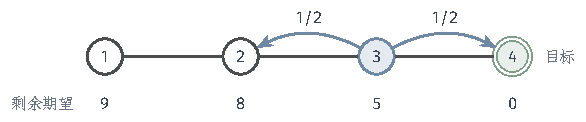
\includegraphics[width=99.24mm]{figures/03-graphs/05-matrices-and-spectra/tikz/walk-examples/hitting-path-target.pdf}
\caption{四顶点单位权路径以$4$为目标。节点下方是以该点为起点还要走的期望步数。箭头标出从$3$出发的两个去处及其概率，双圈标出目标。}
\label{fig:graph-walk-hitting-target}
\end{BookInlineFigure}

\paragraph{两个方向的首达期望不同}

从$1$到$2$只需一步。反过来从$2$到$1$就不一样了：$2$有$1/2$的概率直接到$1$，另有$1/2$的概率先走到$3$。走到$3$之后，要先从$3$绕回$2$，然后再重新尝试。

先算从$3$到$2$的平均时间。从$3$出发，$1/2$概率一步到$2$，$1/2$概率走到$4$。走到$4$后下一步必回$3$，等于白走两步回到原处。因此
\[
h_{3,2}=\tfrac{1}{2}\cdot1+\tfrac{1}{2}(2+h_{3,2}).
\]
解得$h_{3,2}=3$。

回到从$2$到$1$的问题。$1/2$概率一步到达，$1/2$概率先到$3$（一步），再从$3$回到$2$（平均$3$步），然后重新开始，
\[
h_{2,1}=\tfrac{1}{2}\cdot1+\tfrac{1}{2}(1+3+h_{2,1}).
\]
解得$h_{2,1}=5$。虽然$\{1,2\}$是一条无向边，但从两端出发绕远的机会完全不同。

在完全图$K_n$上，只要尚未命中目标，从任何非目标顶点出发，下一步命中的概率都是$1/(n-1)$。等待步数的期望就是$n-1$。

\subsection{往返时间与有效电阻}
\label{sec:graph-walk-commute-resistance}

从$i$去$j$再从$j$回$i$，总等待时间由两段组成。前一段的期望是$h_{i,j}$。前一段结束时，棋子恰好在$j$，此后每一步仍按相同规则转移，返程的条件期望都是$h_{j,i}$。两段相加，\term{往返时间}（commute time）的期望为$h_{i,j}+h_{j,i}$。

单向首达期望不对称。为了找到一个对称的表达式，先把首达方程恢复成全图形式。

将$\bm{L}\bm{h}_{:,j}$的各分量相加。$\bm{L}$的每一列和为零，因此总和也为零。已知$i\ne j$时第$i$项等于$d_i$，所以第$j$项必须抵消其余各项之和，等于$d_j-\operatorname{vol}(V)$。用$\bm{e}_j$记第$j$项为$1$、其余为$0$的列向量，全图方程为
\begin{equation}
\bm{L}\bm{h}_{:,j}=\bm{d}-\operatorname{vol}(V)\bm{e}_j.
\label{eq:graph-walk-full-hitting}
\end{equation}

右端各分量和为零，可以用伪逆$\bm{L}^\dagger$先求一个解。$\bm{L}^\dagger\bm{e}_j$取出伪逆的第$j$列，因此
\[
\bm{x}=\bm{L}^\dagger\bm{d}-\operatorname{vol}(V)\bm{L}^\dagger\bm{e}_j.
\]
这个解的第$j$项未必为零。由$\bm{L}\bm{1}=\bm{0}$，可以统一减去$x_j$后仍满足方程，同时保证$h_{j,j}=0$。展开$h_{i,j}=x_i-x_j$，得
\begin{equation}
h_{i,j}=(\bm{L}^\dagger\bm{d})_i-(\bm{L}^\dagger\bm{d})_j
+\operatorname{vol}(V)
\bigl((\bm{L}^\dagger)_{j,j}-(\bm{L}^\dagger)_{i,j}\bigr).
\label{eq:graph-walk-hitting-pseudoinverse}
\end{equation}
第一行包含度向量的信息，记录了度分配对单向首达时间的影响。正则图上度为常向量，这一部分消失。

把去程和返程相加。交换$i,j$后，第一行的两个差值恰好符号相反，抵消为零。剩下的是总加权度乘
\[
(\bm{L}^\dagger)_{i,i}+(\bm{L}^\dagger)_{j,j}
-(\bm{L}^\dagger)_{i,j}-(\bm{L}^\dagger)_{j,i}.
\]
把差向量$\bm{e}_i-\bm{e}_j$放在$\bm{L}^\dagger$的两侧相乘，展开后恰好是这四项。这正是第~\ref{sec:graph-effective-resistance}节的有效电阻二次型。

\begin{theorem}[往返时间与有效电阻]
\label{thm:graph-walk-commute-resistance}
对正权支撑连通的有限无向图，任意两点$i,j$的往返期望为
\begin{equation}
h_{i,j}+h_{j,i}
=\operatorname{vol}(V)\,R_{i,j}.
\label{eq:graph-walk-commute-time}
\end{equation}
\end{theorem}

有效电阻衡量一对顶点间的电势响应，乘以总加权度后就给出两次首达所需的平均总步数。

在四点路径上，总加权度为$1+2+2+1=6$。相邻点$1,2$之间只有一条单位电阻边，$R_{1,2}=1$，往返期望为$6$，与$h_{1,2}+h_{2,1}=1+5$一致。两端之间串联三条边，$R_{1,4}=3$，往返期望为$18$，即两个方向各$9$步。

在$n$点单位权环上，若两点沿环相隔$k$条边，两段弧的电阻分别为$k$和$n-k$，并联后得到$R=k(n-k)/n$。总度为$2n$，往返期望为$2k(n-k)$。

若把所有电导同时乘$c>0$，每步用边权除以度，转移矩阵保持不变。电阻缩小为原来的$1/c$，总加权度增为$c$倍，二者相乘后仍不变。

\section{遍历时间}
\label{sec:graph-walk-cover}

想象每到一个顶点就给它做上记号。走过已标记的顶点花了一步但没有新记号。遍历问题关心最后一个记号何时出现。

\subsection{遍历时间的计算}
\label{sec:graph-walk-cover-computation}

把起点计为已访问，定义\term{遍历时间}（cover time）$\tau_{\mathrm{cov}}$，分别记从$i$出发的遍历期望$C_i$和最坏起点的期望$C$，
\begin{equation}
\begin{aligned}
\tau_{\mathrm{cov}}&=\inf\{t\ge0:\{X_0,\ldots,X_t\}=V\},\\
C_i&=\mathbb{E}_i[\tau_{\mathrm{cov}}],
\qquad C=\max_i C_i.
\end{aligned}
\label{eq:graph-walk-cover-definition}
\end{equation}
遍历要求所有顶点都被访问，不要求每条边都经过。

\paragraph{完全图上的逐阶段收集}

在$K_n$的单位权游走中，若已经标记了$k$个顶点，当前顶点之外有$n-1$个等可能的去处，其中$n-k$个尚未标记。一步找到新顶点的概率为$p=(n-k)/(n-1)$。

只要这一步没有找到新顶点，记号数仍为$k$，下一步的情况完全一样。等待时间的期望$H$满足
\[
H=1+(1-p)H.
\]
式中$1$是必走的一步，$1-p$是失败后继续等$H$步。因此$H=1/p$。

将从$k$个记号增加到$k+1$个所需的平均步数$1/p=(n-1)/(n-k)$，按$k$从$1$到$n-1$相加。令$j=n-k$表示还未访问的顶点数，得到
\begin{equation}
C_i=(n-1)\sum_{j=1}^{n-1}\frac{1}{j}.
\label{eq:graph-walk-cover-complete}
\end{equation}
例如$K_4$的三段期望为$3/3=1$、$3/2$、$3/1=3$，合计$11/2$步。

\paragraph{路径端点的遍历}

在单位权$n$点路径上从端点$1$出发，首次到达另一端$n$之前必然经过所有中间顶点。因此$C_1=h_{1,n}$。两端之间串联了$n-1$条单位电阻边，$R_{1,n}=n-1$，总加权度$\operatorname{vol}(V)=2(n-1)$。路径反转后形状一样，所以$h_{1,n}=h_{n,1}$，由往返公式$2h_{1,n}=2(n-1)(n-1)$，得
\[
C_1=h_{1,n}=(n-1)^2.
\]
若起点在内部，遍历还需要覆盖两端，下一小节给出的统一上界可以处理任意起点。

\subsection{生成树上界}
\label{sec:graph-walk-cover-tree-bound}

一般图上很难直接按已访问集合分阶段计算，因为同样数量的记号可能分布在完全不同的区域。一种做法是：指定一份覆盖全图的访问次序，估计完成它所需的时间。由于实际遍历可能更早结束，这份次序给出的是遍历时间的上界。

以起点$u$为根取一棵生成树$T$，沿深度优先次序走完这棵树。每条树边去一次、回一次，沿途列出必须依次命中的目标。

例如四点环加对角线$\{1,3\}$，选择树路径$1\!-\!2\!-\!3\!-\!4$，从$1$出发的目标名单为$2,3,4,3,2,1$。这份名单只规定停止条件：先等到$2$、再等到$3$，以此类推。等待期间，棋子仍在原图上随机走，可以经过对角线。图~\ref{fig:graph-walk-cover-tree-targets}把所选的树和由它生成的名单放在一起。

\begin{BookInlineFigure}
\centering
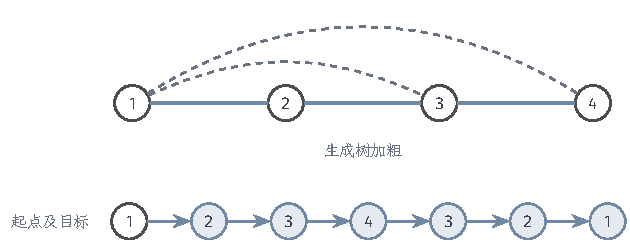
\includegraphics[width=106.726mm]{figures/03-graphs/05-matrices-and-spectra/tikz/walk-examples/cover-tree-targets.pdf}
\caption{用四点环加对角线$\{1,3\}$说明遍历上界。粗实线是所选树边，虚线是原图的其余边。下方从白底的起点$1$开始，箭头依次指向六个等待目标。实际游走仍可沿原图的所有边转移。}
\label{fig:graph-walk-cover-tree-targets}
\end{BookInlineFigure}

命中当前目标后，棋子的位置已经确定。下一段等待的期望就是从该位置出发的首达期望，与此前走过哪些顶点无关。

按名单完成全部目标时，每个顶点一定都已访问过。实际遍历可能更早结束——某些顶点在正式等到它之前已经顺路走过。因此名单给出的总等待时间是一个上界。

将每条树边的去程和返程配对，利用往返公式~\eqref{eq:graph-walk-commute-time}，得到
\begin{equation}
C_u\le\sum_{\{a,b\}\in T}(h_{a,b}+h_{b,a})
=\operatorname{vol}(V)\sum_{\{a,b\}\in T}R_{a,b}.
\label{eq:graph-walk-cover-resistance}
\end{equation}

每条树边$\{a,b\}$本身已经存在于图中。将全部单位电流送过这条边，可行流的耗散为$1/w_{a,b}$。有效电阻是所有单位流的最小耗散，因此$R_{a,b}\le1/w_{a,b}$。

对无权图，每条树边的$R_{a,b}\le1$，树有$n-1$条边，总加权度为$2m$，于是
\begin{equation}
C\le2m(n-1).
\label{eq:graph-walk-cover-unweighted}
\end{equation}
路径图的$m=n-1$，从端点出发的下界$(n-1)^2$与上界$2(n-1)(n-1)$同阶，因此最坏起点的遍历期望为$\Theta(n^2)$。

\paragraph{三次方量级的构造}

取一个$k$点完全图，在其中一个顶点$u$上接出一条含$\ell$条边的路径，末端为$v$。路径上所有边串联在$u,v$之间，完全图只在$u$处与路径相接，无法分担通往$v$的电流，因此$R_{u,v}=\ell$。

完全图已有$k(k-1)/2$条边，路径增加$\ell$条，每条边两端都计入度数，总加权度为$k(k-1)+2\ell$。

从$v$出发首次到达$u$以前，棋子只能在路径上行走，故$h_{v,u}=\ell^2$。利用往返公式减去这一方向，得
\[
h_{u,v}=\operatorname{vol}(V)\,R_{u,v}-h_{v,u}
=(k(k-1)+2\ell)\ell-\ell^2=k(k-1)\ell+\ell^2.
\]
遍历至少要到达$v$。当$k$与$\ell$都和$n=k+\ell$同阶时，这一项给出$\Theta(n^3)$的下界，与式~\eqref{eq:graph-walk-cover-unweighted}的上界量级一致。大量边集中在一个团里，增加了找到路径入口前的等待。

\section{PageRank}
\label{sec:graph-pagerank}

把网页看成顶点，链接看成有向边。只沿链接行走时，棋子可能进入走不出来的区域，也可能来到没有出边的页面。给行走加入重新选择顶点的机会，可以用长期分布为页面排名。这种做法称为\term{PageRank}\scite{page1999pagerank}。

\subsection{PageRank方程}
\label{sec:graph-pagerank-equation}

\paragraph{有向图的转移矩阵}

有向图的弧只从尾端指向头端。计算顶点$i$的转移概率时，只读取从$i$出去的弧，按出弧权重的总和归一化。

若某个顶点没有出边，就没有权重可以归一化。设$\bm{s}$为给定的概率行，用它补上零出度顶点所在的行。补齐后的$\bm{P}$每行非负、和为一，是一个行随机矩阵。

\paragraph{平稳分布的存在}

有限行随机矩阵总有平稳分布。为说明这一点，取任意概率初态$\bm{\nu}^{(0)}$，把前$T$步的分布取平均，
\[
\bm{a}^{(T)}=\frac{1}{T}\sum_{t=0}^{T-1}\bm{\nu}^{(0)}\bm{P}^t.
\]
右乘$\bm{P}$将每个时刻推进一步，新平均覆盖第$1$到第$T$步。中间$T-1$项相同，首尾两项之差除以$T$趋于零，
\[
\bm{a}^{(T)}\bm{P}-\bm{a}^{(T)}
=\frac{\bm{\nu}^{(0)}\bm{P}^T-\bm{\nu}^{(0)}}{T}
\to\bm{0}.
\]
这些平均都是概率行，位于有限维的闭有界集合中。从中选出一个收敛子列，极限就是平稳分布。

\paragraph{不唯一和振荡}

存在平稳分布之后，还要问它是否唯一、迭代能否收敛到它。

两个互不相连的有向环各有一个平稳分布，初态的分配方式会影响极限。即使平稳解唯一，迭代也可能振荡——一个两点有向环的唯一平稳分布是$(1/2,1/2)$，但从一点出发，分布在两个顶点之间永远交替。

\paragraph{重启机制}

为了同时解决不唯一和振荡，在每一步独立决定是否重启。以概率$\alpha\in(0,1)$按$\bm{s}$选择新位置，以概率$1-\alpha$按补齐后的$\bm{P}$转移。重启这一支不依赖当前位置，总使用同一份$\bm{s}$。

如果当前分布为$\bm{p}$，两支分别向下一步贡献$\alpha\bm{s}$和$(1-\alpha)\bm{p}\bm{P}$。要求下一步仍是$\bm{p}$，得到
\begin{equation}
\bm{p}=\alpha\bm{s}+(1-\alpha)\bm{p}\bm{P}.
\label{eq:graph-pagerank-fixed-point}
\end{equation}

这个方程还有另一种理解方式。先按$\bm{s}$选起点，每到一个位置，以概率$\alpha$结束，否则按$\bm{P}$再走一步。绕过前$t$次结束机会才在第$t+1$次结束，行走恰好走了$t$步，概率为$\alpha(1-\alpha)^t$。终点分布按步数加权求和，得
\begin{equation}
\bm{p}=\alpha\sum_{t=0}^{\infty}(1-\alpha)^t\bm{s}\bm{P}^t.
\label{eq:graph-pagerank-series}
\end{equation}
第零项对应立即结束的$\alpha\bm{s}$。把其余各项整体前移一个步数，提出公因子$(1-\alpha)$和一次$\bm{P}$，恰好得到$(1-\alpha)\bm{p}\bm{P}$。两部分相加满足式~\eqref{eq:graph-pagerank-fixed-point}。

\paragraph{唯一性与收敛性}

对任意两份概率差$\bm{z}$，一步转移不会放大$\ell^1$距离：逐列取绝对值并利用行和为一，$\lVert\bm{z}\bm{P}\rVert_1\le\lVert\bm{z}\rVert_1$。式~\eqref{eq:graph-pagerank-fixed-point}右端的更新映射$F$满足
\begin{equation}
\lVert F(\bm{x})-F(\bm{y})\rVert_1
\le(1-\alpha)\lVert\bm{x}-\bm{y}\rVert_1.
\label{eq:graph-pagerank-contraction}
\end{equation}
这是因为两个输入共享同一份重启$\alpha\bm{s}$，差值只出现在$1-\alpha$比例的转移部分。

若存在两个平稳解，更新后它们不变、距离不变，但收缩系数$1-\alpha<1$迫使距离为零。唯一性得证。从任意初态出发，第$t$轮与真解的距离每轮至少缩小为$1-\alpha$倍，因此迭代收敛。

\subsection{算法实现}
\label{sec:graph-pagerank-implementation}

输入为有向邻接表、概率行$\bm{s}$、重启概率$\alpha$和$\ell^1$误差容限$\varepsilon$。算法维护一份候选排名$\bm{p}^{(t)}$，从$\bm{p}^{(0)}=\bm{s}$开始。每一轮先沿实际出边传播概率，再加上重启部分。

\begin{algorithm}[PageRank迭代]
\label{alg:graph-pagerank-iteration}
输入：有向邻接表、概率行$\bm{s}$、重启概率$\alpha$、容许$\ell^1$误差$\varepsilon$。输出：近似排名$\bm{p}$。
\begin{enumerate}
  \item 令$\bm{p}^{(0)}=\bm{s}$。对零出度顶点记录标志。
  \item 每轮执行更新$\bm{p}^{(t+1)}=\alpha\bm{s}+(1-\alpha)\bm{p}^{(t)}\bm{P}$。实现时：先对每个正出度顶点$i$，把$(1-\alpha)p^{(t)}_i$按出边权重比例分给各头端。同时累计所有零出度顶点上的质量$q$，统一加回$q\bm{s}$。最后再加上重启项$\alpha\bm{s}$。
  \item 计算残差$\bm{r}=\bm{p}^{(t+1)}-\bm{p}^{(t)}$。若$\lVert\bm{r}\rVert_1\le\alpha\varepsilon$，返回$\bm{p}^{(t+1)}$。
\end{enumerate}
\end{algorithm}

每轮更新写成公式为
\begin{equation}
\bm{p}^{(t+1)}=\alpha\bm{s}+(1-\alpha)\bm{p}^{(t)}\bm{P}.
\label{eq:graph-pagerank-iteration}
\end{equation}

每轮先沿实际出边传播概率。对于零出度的顶点，只把它的分数加到悬挂质量$q$中。边扫描结束后，统一把$q\bm{s}$加到尚未乘$1-\alpha$的一步结果中。这等价于给每个悬挂点补上同一行$\bm{s}$，只需存一份重启分布。

考虑四个顶点及单位权弧$1\to2$、$2\to3$、$3\to1$、$3\to4$。顶点$4$没有出边。取$\bm{s}=(1,0,0,0)$、$\alpha=1/2$。每轮的重启部分给顶点$1$增加$1/2$的质量。

第一轮开始时全部质量在$1$，沿边部分的$1/2$送往$2$。第二轮将顶点$1$的质量减半后送到$2$，同时将$2$的质量减半后送到$3$，两点各得$1/4$。第三轮中，顶点$3$的$1/4$里有$1/2$沿边分出，分给$1,4$各$1/16$。这是顶点$4$首次收到质量。各轮结果为
\[
\begin{array}{c@{\qquad}c}
t&\bm{p}^{(t)}\\
1&(1/2,1/2,0,0)\\
2&(1/2,1/4,1/4,0)\\
3&(9/16,1/4,1/8,1/16)\\
4&(9/16,9/32,1/8,1/32)
\end{array}
\]
第四轮中，顶点$4$的旧质量$1/16$通过零出度填补分给顶点$1$，再乘沿边比例$1/2$，贡献$1/32$。同轮$3$也沿弧$3\to1$送来$1/32$。重启的$1/2$加上这两笔，$1$的新质量为$9/16$。图~\ref{fig:graph-pagerank-fourth-round}给出这一轮的各笔转移。

\begin{BookInlineFigure}
\centering
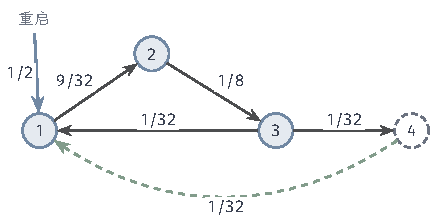
\includegraphics[width=73.459mm]{figures/03-graphs/05-matrices-and-spectra/tikz/walk-examples/pagerank-fourth-round.pdf}
\caption{四页算例在第四轮的质量分配，重启概率为$1/2$，重启集中到顶点$1$。深灰实线沿实际链接送出质量，虚线是零出度顶点$4$补齐后送出的份额。重启直接增加顶点$1$的质量。}
\label{fig:graph-pagerank-fourth-round}
\end{BookInlineFigure}

每轮所得各项非负，总和应为一，可据此检查传播、悬挂补偿和重启项是否漏加。

\subsection{算法分析}
\label{sec:graph-pagerank-cost}

由式~\eqref{eq:graph-pagerank-contraction}及两份概率行的$\ell^1$距离至多为$2$，第$t$轮的误差满足
\begin{equation}
\lVert\bm{p}^{(t)}-\bm{p}\rVert_1\le 2(1-\alpha)^t.
\label{eq:graph-pagerank-geometric-bound}
\end{equation}
要将上界压到$\varepsilon$，对$2(1-\alpha)^t\le\varepsilon$取对数，得到充分的迭代轮数
\[
t\ge \left\lceil\frac{\log(2/\varepsilon)}{-\log(1-\alpha)}\right\rceil.
\]
例如$\alpha=1/2$时，六轮可把上界压到$1/32$。当$\alpha$很小时，$-\log(1-\alpha)$与$\alpha$同阶，轮数约为$\alpha^{-1}\log(2/\varepsilon)$。

在运行中，真解$\bm{p}$未知，但可以计算候选$\bm{q}$再走一轮会变多少。记残差为$\bm{r}=F(\bm{q})-\bm{q}$。从$\bm{q}$到真解$\bm{p}$的距离，可以先走到$F(\bm{q})$再走到$F(\bm{p})=\bm{p}$。第一段距离是$\lVert\bm{r}\rVert_1$，第二段由收缩性控制，因此
\[
\lVert\bm{q}-\bm{p}\rVert_1
\le\lVert\bm{r}\rVert_1+(1-\alpha)\lVert\bm{q}-\bm{p}\rVert_1.
\]
移项得到
\begin{equation}
\lVert\bm{q}-\bm{p}\rVert_1\le\frac{\lVert\bm{r}\rVert_1}{\alpha}.
\label{eq:graph-pagerank-residual-bound}
\end{equation}
若残差范数不超过$\alpha\varepsilon$，当前候选的误差就不超过$\varepsilon$。

设图有$n$个顶点、$m$条弧。每轮传播扫描$m$条弧，初始化和悬挂补偿需$O(n)$。每轮时间和整个存储均为$O(n+m)$。

$\alpha$越大，一次行走越可能很快结束，终点分布越接近$\bm{s}$，迭代也越快收敛。较小的$\alpha$留下更多沿边传播的机会，但也让每轮保留更多旧误差。选择$\alpha$同时改变排名的含义和计算的速度。

\section{个性化PageRank}
\label{sec:graph-personalized-pagerank}

上一节的标准PageRank取均匀跳转分布$\bm s=\frac1n\bm 1^\top$，计算出的是所有节点与查询者无关的“全局通用权威分”。如果我们将重启分布$\bm s$集中到某一个指定节点$u$（或少数几个节点）上，让随机游走每次重启时都回到$u$重新出发，所得的平稳分布就称为\term{个性化PageRank}（personalized PageRank，简称PPR），其中的起点称为\term{种子}（seed）。本节按照“背景与主要思想—算法实现—算法分析”的脉络，介绍个性化PageRank及其在超大规模图上的局部推送算法与局部谱划分应用。

\subsection{背景与主要思想}
\label{sec:graph-pagerank-push-principle}

\paragraph{为什么引入个性化PageRank}

全局排名与针对某个种子的关联排名回答不同的问题。将重启分布集中在顶点$u$后，游走反复从$u$出发，短路径的传播权重通常高于长路径。个性化PageRank由图结构、转移概率与重启概率共同确定，因而可作为相对于种子的关联度量；它不等同于最短路距离，也不保证得分高的顶点一定与种子直接相邻。

第二个问题是如何利用稀疏种子进行局部计算。全局幂迭代通常读取整张图，而局部查询未必需要计算每个顶点的精确分数。重启使长度为$t$的传播项按几何因子衰减，但这不自动保证某个小邻域包含绝大多数概率质量。下面的局部推送通过截断单位度数余量，给出显式的工作量与误差界；在参数和种子支撑较小时，它可能只访问图的一部分。

\paragraph{主要思想：种子重启与局部推送（Local Push）}

本节在至少有两个顶点的连通简单无权图上考察采用惰性转移矩阵$\bm Q=(\bm I+\bm P)/2$的个性化PageRank。在个性化PageRank与局部算法文献中，习惯用$\alpha\in(0,1)$直接表示每一步的\emph{重启（或就地终止）概率}，用$1-\alpha$表示沿惰性矩阵$\bm Q$继续游走一步的概率（对应上一节的阻尼系数$1-\alpha$）。对于任意非负种子向量$\bm s\in\mathbb R^{1\times n}$（通常取单点种子$\bm s=\bm e_u^\top$），对应的个性化PageRank线性算子$\mathcal R(\bm s)$定义为
\begin{equation}
\mathcal{R}(\bm{s})
=\alpha\sum_{t=0}^{\infty}(1-\alpha)^t\bm{s}\bm{Q}^t,
\label{eq:graph-pagerank-linear-operator}
\end{equation}
其满足不动点方程$\mathcal R(\bm s)=\alpha\bm s+(1-\alpha)\mathcal R(\bm s)\bm Q$，且对任意待分配质量行向量$\bm r$满足一步分解恒等式：
\begin{equation}
\mathcal{R}(\bm{r})=\alpha\bm{r}+(1-\alpha)\mathcal{R}(\bm{r}\bm{Q}).
\label{eq:graph-pagerank-push-decomposition}
\end{equation}

如何在不扫描全图的前提下算出$\mathcal R(\bm s)$的高精度近似？Andersen、Chung与Lang于2006年提出了著名的\emph{局部推送}（local push，或ApproximatePR）思想\scite{andersen2006localpagerank}。

其核心设计首先在于\emph{维护“已确认分数$\bm p$ + 待处理余量$\bm r$”的质量守恒不变量}。局部推送不像全局幂法那样每轮同步更新全图所有节点，而是维护两个稀疏行向量：一个是记录已经终止游走、已累积的终点分数的\emph{近似向量}$\bm p$，另一个是记录当前仍滞留在各节点等待继续向外扩散的\emph{余量向量}（residual）$\bm r$。初始时令已确认分数$\bm p=\bm 0$，并将全部初始种子质量放入待处理余量$\bm r=\bm s$。

在每一步局部操作中，算法只单独挑出一个节点$i$，将它当前积压的余量$q=r_i$清空，并按一步分解式~\eqref{eq:graph-pagerank-push-decomposition}拆成两部分处理：其中$\alpha q$比例就地停止游走，直接累加到已确认分数$p_i$中；其余$(1-\alpha)q$比例则按惰性矩阵$\bm Q$向前推进一步，分发给节点$i$自身及它的直接邻居作为新的待处理余量。

由于每次推送只是把单个节点$i$的待处理质量沿着随机游走规则向前推进了一步，整个算法运行期间始终严格保持如下质量守恒不变量：
\begin{equation}
\mathcal{R}(\bm{s})=\bm{p}+\mathcal{R}(\bm{r}).
\label{eq:graph-pagerank-push-invariant}
\end{equation}

对顶点$i$推送一次需读取$d_i$个邻居。用阈值$r_i/d_i>\varepsilon$筛选活跃顶点，便能将每次读取的邻接表大小与被转移到$\bm p$中的质量联系起来。当所有余量均满足$r_i\leq\varepsilon d_i$时停止，可得到逐点误差界。算法不必展开所有顶点的邻接表，但仍会读取被推送顶点的邻居标识并更新余量；是否为亚线性工作量取决于$\alpha,\varepsilon$和种子支撑。

\subsection{算法实现}
\label{sec:graph-pagerank-push-implementation}

\paragraph{局部推送算法步骤}

在简单无权图上，惰性转移矩阵$\bm Q=(\bm I+\bm P)/2$将一半质量留在当前顶点$i$，另一半质量均分给$i$的$d_i$个邻居。因此，对顶点$i$（旧余量记为$q=r_i$）执行一次局部推送的更新公式为
\begin{equation}
\begin{aligned}
p_i &\leftarrow p_i+\alpha q,\\
r_i &\leftarrow (1-\alpha)q/2,\\
r_j &\leftarrow r_j+(1-\alpha)q/(2d_i),\qquad \forall j\sim i.
\end{aligned}
\label{eq:graph-pagerank-push-update}
\end{equation}
采用哈希表（字典）稀疏存储$\bm p$与$\bm r$，并用队列维护满足$r_i>\varepsilon d_i$的活跃顶点，完整算法如下。

\begin{algorithm}[个性化PageRank局部推送（Local Push）]
\label{alg:graph-personalized-pagerank-push}
输入：可按点查询且能常数时间读取度数的无向图邻接表、稀疏种子分布$\bm{s}$、重启概率$\alpha\in(0,1)$、截断阈值$\varepsilon>0$。输出：稀疏近似分数$\bm{p}$与剩余余量$\bm{r}$。
\begin{enumerate}
  \item \textbf{稀疏初始化}：令$\bm{p}=\bm{0}$、$\bm{r}=\bm{s}$。将所有满足$r_i>\varepsilon d_i$的顶点$i$加入活跃队列$Q$。
  \item \textbf{局部推送循环}：当队列$Q$非空时，弹出队首顶点$i$，记其当前余量为$q=r_i$，按式~\eqref{eq:graph-pagerank-push-update}执行局部推送：
    \begin{enumerate}
    \item 划入已确认分数：$p_i\leftarrow p_i+\alpha q$；
    \item 更新本点惰性停留余量：$r_i\leftarrow(1-\alpha)q/2$；
    \item 分发邻居余量：遍历$i$的每个邻居$j\sim i$，令$r_j\leftarrow r_j+(1-\alpha)q/(2d_i)$。
    \end{enumerate}
    更新完毕后，检查顶点$i$及每个邻居$j\sim i$：若某个顶点满足$r_v>\varepsilon d_v$且不在队列$Q$中，将其加入队尾。
  \item \textbf{终止返回}：当队列$Q$为空时停止，返回稀疏向量$\bm{p}$和$\bm{r}$。
\end{enumerate}
\end{algorithm}

\paragraph{四点路径上的三次推送演示}

在单位权四点路径$1\!-\!2\!-\!3\!-\!4$上取单点种子$1$（$\bm s=(1,0,0,0)$），重启概率$\alpha=1/2$，阈值$\varepsilon=1/8$。四个顶点的度依次为$1,2,2,1$，对应的触发阈值$\varepsilon d_i$依次为$\frac18,\frac14,\frac14,\frac18$。
\begin{itemize}
\item \emph{第一次推送顶点$1$}：旧余量$q=1>\frac18$。划入分数$p_1\leftarrow\frac12$；剩余$\frac12$对半分，$r_1\leftarrow\frac14$留在本点，$r_2\leftarrow\frac14$送给邻居$2$，此时$\bm p=(\frac12,0,0,0),\bm r=(\frac14,\frac14,0,0)$。因$r_1=\frac14>\frac18$仍超阈值，顶点$1$继续留在队列中（而$r_2=\frac14$未严格超过$\varepsilon d_2=\frac14$）。
\item \emph{第二次推送顶点$1$}：旧余量$q=\frac14$。划入分数$\frac18$使$p_1=\frac58$；剩余$\frac18$对半分，$r_1\leftarrow\frac{1}{16}$，$r_2\leftarrow\frac14+\frac{1}{16}=\frac{5}{16}$。此时$\bm p=(\frac58,0,0,0),\bm r=(\frac{1}{16},\frac{5}{16},0,0)$，顶点$2$的余量$\frac{5}{16}>\frac14$超过阈值，进入队列。
\item \emph{第三次推送顶点$2$}（图~\ref{fig:graph-pagerank-third-push}）：旧余量$q=\frac{5}{16}$。划入分数$p_2\leftarrow\frac{5}{32}$；剩余$\frac{5}{32}$中一半$\frac{5}{64}$留作$r_2$，另一半$\frac{5}{64}$均分给邻居$1$和$3$（各加$\frac{5}{128}$）。合并后得到
\[
\bm{p}=\left(\frac58,\frac{5}{32},0,0\right),\qquad
\bm{r}=\left(\frac{13}{128},\frac{5}{64},\frac{5}{128},0\right).
\]
此时四个顶点的余量均不再超过各自阈值$\frac18,\frac14,\frac14,\frac18$，队列为空，算法终止。注意最右端的顶点$4$在整个运行过程中从未被访问过（$p_4=r_4=0$）。图~\ref{fig:pagerank-push-evolution}以柱状图直观展示了三次推送中$\bm p$与$\bm r$的消长过程。
\end{itemize}

\begin{BookInlineFigure}
\centering
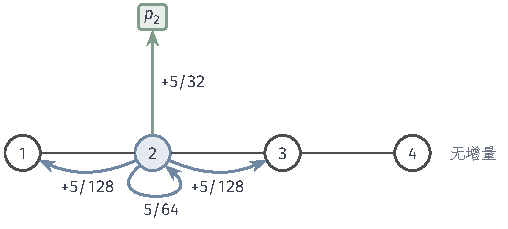
\includegraphics[width=85.965mm]{figures/03-graphs/05-matrices-and-spectra/tikz/walk-examples/pagerank-push-path.pdf}
\caption{四顶点路径上的第三次局部推送（$\alpha=1/2$）。从顶点$2$取出旧余量$5/16$：向上箭头将$5/32$确认为终点分数$p_2$，回环将$5/64$留作本点余量，左右箭头向邻居$1,3$各分发$5/128$余量。}
\label{fig:graph-pagerank-third-push}
\end{BookInlineFigure}

\begin{figure}[!htb]
\centering
\begin{tikzpicture}[x=1mm,y=1mm,
  pbar/.style={fill=FigureBlueFill,draw=FigureBlue,line width=.4pt},
  rbar/.style={fill=FigureYellowFill,draw=FigureYellow,line width=.4pt},
  panel/.style={anchor=mid,font=\figurefont\footnotesize},
  vlabel/.style={font=\figurefont\fontsize{6.5}{8}\selectfont,FigureInk,anchor=north},
  plabel/.style={font=\figurefont\fontsize{6}{7.5}\selectfont,FigureInk,anchor=south}]
  \def\bw{2.6}
  \def\sc{32}
  \def\gp{1.2}
  \def\vgp{3.0}
  \fill[pbar] (0,27) rectangle +(3,2); \node[font=\figurefont\fontsize{6.5}{8}\selectfont,anchor=west] at (4,28) {分数$p_i$};
  \fill[rbar] (20,27) rectangle +(3,2); \node[font=\figurefont\fontsize{6.5}{8}\selectfont,anchor=west] at (24,28) {余量$r_i$};
  \begin{scope}[xshift=0mm]
    \draw[FigureStroke,line width=.35pt] (0,0) -- (0,\sc*0.55);
    \draw[FigureStroke,line width=.35pt] (0,0) -- (4*2*\bw+4*\gp+3*\vgp+1,0);
    \foreach \i/\v/\pv/\rv in {0/1/0.5/0.25, 1/2/0/0.25, 2/3/0/0, 3/4/0/0} {
      \pgfmathsetmacro{\x}{\i*(2*\bw+\gp+\vgp)+1}
      \pgfmathsetmacro{\hp}{\pv*\sc}
      \pgfmathsetmacro{\hr}{\rv*\sc}
      \pgfmathparse{\pv>0?1:0}\ifnum\pgfmathresult=1
        \fill[pbar] (\x,0) rectangle +(\bw,\hp);
      \fi
      \pgfmathparse{\rv>0?1:0}\ifnum\pgfmathresult=1
        \fill[rbar] (\x+\bw+\gp,0) rectangle +(\bw,\hr);
      \fi
      \node[vlabel] at (\x+\bw+\gp/2,-1) {$\v$};
    }
    \node[panel] at (15,-7) {(a) 第$1$次推送后};
  \end{scope}
  \begin{scope}[xshift=36mm]
    \draw[FigureStroke,line width=.35pt] (0,0) -- (0,\sc*0.7);
    \draw[FigureStroke,line width=.35pt] (0,0) -- (4*2*\bw+4*\gp+3*\vgp+1,0);
    \foreach \i/\v/\pv/\rv in {0/1/0.625/0.0625, 1/2/0/0.3125, 2/3/0/0, 3/4/0/0} {
      \pgfmathsetmacro{\x}{\i*(2*\bw+\gp+\vgp)+1}
      \pgfmathsetmacro{\hp}{\pv*\sc}
      \pgfmathsetmacro{\hr}{\rv*\sc}
      \pgfmathparse{\pv>0?1:0}\ifnum\pgfmathresult=1
        \fill[pbar] (\x,0) rectangle +(\bw,\hp);
      \fi
      \pgfmathparse{\rv>0?1:0}\ifnum\pgfmathresult=1
        \fill[rbar] (\x+\bw+\gp,0) rectangle +(\bw,\hr);
      \fi
      \node[vlabel] at (\x+\bw+\gp/2,-1) {$\v$};
    }
    \node[panel] at (15,-7) {(b) 第$2$次推送后};
  \end{scope}
  \begin{scope}[xshift=72mm]
    \draw[FigureStroke,line width=.35pt] (0,0) -- (0,\sc*0.7);
    \draw[FigureStroke,line width=.35pt] (0,0) -- (4*2*\bw+4*\gp+3*\vgp+1,0);
    \foreach \i/\v/\pv/\rv in {0/1/0.625/0.1016, 1/2/0.1563/0.0781, 2/3/0/0.0391, 3/4/0/0} {
      \pgfmathsetmacro{\x}{\i*(2*\bw+\gp+\vgp)+1}
      \pgfmathsetmacro{\hp}{\pv*\sc}
      \pgfmathsetmacro{\hr}{\rv*\sc}
      \pgfmathparse{\pv>0?1:0}\ifnum\pgfmathresult=1
        \fill[pbar] (\x,0) rectangle +(\bw,\hp);
      \fi
      \pgfmathparse{\rv>0?1:0}\ifnum\pgfmathresult=1
        \fill[rbar] (\x+\bw+\gp,0) rectangle +(\bw,\hr);
      \fi
      \node[vlabel] at (\x+\bw+\gp/2,-1) {$\v$};
    }
    \node[panel] at (15,-7) {(c) 第$3$次推送后};
  \end{scope}
\end{tikzpicture}
\caption{四点路径上三次局部推送后的已确认分数$\bm{p}$（蓝色）与待处理余量$\bm{r}$（黄色）。每次推送仅在局部更新被推顶点及其邻居，远端顶点$4$始终未被触及。}
\label{fig:pagerank-push-evolution}
\end{figure}

\subsection{算法分析}
\label{sec:graph-pagerank-push-analysis}

下面证明局部推送的邻接表访问总量与逐点误差界。推送部分的工作量为$O(1/(\alpha\varepsilon))$，另需读取并初始化种子向量的非零支撑；该上界不显式含$n,m$，但参数随图规模变化时并不保证亚线性。局部划分的质量还需要额外的种子和参数条件。

\begin{theorem}[局部推送算法的复杂度与逐点误差界]
\label{thm:graph-pagerank-push-guarantee}
设在连通简单无权图上对非负种子行向量$\bm s$（$\lVert\bm s\rVert_1\leq 1$）、重启概率$\alpha\in(0,1)$和阈值$\varepsilon>0$运行算法~\ref{alg:graph-personalized-pagerank-push}。则算法必在有限步内停止，且满足：
\begin{enumerate}
  \item \emph{总工作量与支撑集上界}：整个运行过程中所有推送操作访问的邻接表边数总和（及已确认分数$\bm p$的非零支撑集体积）满足
  \begin{equation}
  \operatorname{vol}\bigl(\operatorname{supp}(\bm p)\bigr)
  \le \sum_{\text{各次推送}\;i}d_i
  \le \frac{\lVert\bm s\rVert_1}{\alpha\varepsilon}
  \le \frac{1}{\alpha\varepsilon}.
  \label{eq:graph-pagerank-push-work}
  \end{equation}
  \item \emph{逐点相对度数误差与总质量守恒}：算法停止时输出的$(\bm p,\bm r)$对全图每个顶点$i\in V$满足
  \begin{equation}
  0\le\mathcal{R}(\bm{s})_i-p_i\le\varepsilon d_i,
  \qquad
  \frac{\mathcal{R}(\bm s)_i}{d_i} - \varepsilon \le \frac{p_i}{d_i} \le \frac{\mathcal{R}(\bm s)_i}{d_i},
  \label{eq:graph-pagerank-push-pointwise}
  \end{equation}
  且$\ell^1$总误差恒等于剩余余量的总质量：
  \begin{equation}
  \lVert\mathcal{R}(\bm{s})-\bm{p}\rVert_1=\lVert\bm{r}\rVert_1.
  \label{eq:graph-pagerank-push-mass}
  \end{equation}
\end{enumerate}
\end{theorem}

\begin{proof}
（1）每次从队列中弹出顶点$i$执行推送时，该点必满足触发条件$q=r_i>\varepsilon d_i$。此次推送将$\alpha q>\alpha\varepsilon d_i$的质量从余量$\bm r$转化为已确认分数$\bm p$，而其余$(1-\alpha)q$的质量只是在余量向量内部重新分配，因此余量总和$\lVert\bm r\rVert_1$在此次推送中净减少$\alpha q>\alpha\varepsilon d_i$。由于初始余量总和为$\lVert\bm s\rVert_1\leq 1$且余量始终非负，全部推送操作累计减少的余量不可能超过$\lVert\bm s\rVert_1$：
\[
  \sum_{\text{各次推送}\;i}\alpha\varepsilon d_i \leq \sum_{\text{各次推送}\;i}\alpha q \leq \lVert\bm s\rVert_1\leq 1.
\]
由于每个顶点的度至少为$1$，每次推送至少减少$\alpha\varepsilon$的余量，因此推送次数有限。两边同除以$\alpha\varepsilon$即得式~\eqref{eq:graph-pagerank-push-work}（每个$p_i>0$的顶点至少被推送过一次，故$\operatorname{vol}(\operatorname{supp}(\bm p))\leq\sum d_i\leq\frac{1}{\alpha\varepsilon}$）。

（2）算法停止时队列为空，说明每个顶点$i\in V$的剩余余量均满足$0\leq r_i\leq\varepsilon d_i$，即逐分量有$\bm 0^\top\leq\bm r\leq\varepsilon\bm d^\top$。在无向图上，由详细平衡知度向量满足$\bm d^\top\bm P=\bm d^\top$，从而在惰性矩阵$\bm Q=(\bm I+\bm P)/2$下同样满足平稳性$\bm d^\top\bm Q=\bm d^\top$。因为$\bm Q$的元素全部非负，右乘$\bm Q^t$保持逐分量不等号方向：
\[
  \bm 0^\top\leq\bm r\bm Q^t\leq\varepsilon\bm d^\top\bm Q^t=\varepsilon\bm d^\top\qquad(\forall t\geq 0).
\]
代入级数定义~\eqref{eq:graph-pagerank-linear-operator}并结合守恒不变量~\eqref{eq:graph-pagerank-push-invariant}的$\mathcal R(\bm s)-\bm p=\mathcal R(\bm r)$，立得
\[
  \bm 0^\top\leq\mathcal R(\bm s)-\bm p=\alpha\sum_{t=0}^\infty(1-\alpha)^t\bm r\bm Q^t\leq\alpha\sum_{t=0}^\infty(1-\alpha)^t\varepsilon\bm d^\top=\varepsilon\bm d^\top,
\]
取第$i$个分量即为式~\eqref{eq:graph-pagerank-push-pointwise}。最后，因$\mathcal R(\bm r)\geq\bm 0^\top$且算子$\mathcal R$保持向量分量和不变，有$\lVert\mathcal R(\bm s)-\bm p\rVert_1=\lVert\mathcal R(\bm r)\rVert_1=\lVert\bm r\rVert_1$。
\end{proof}

\paragraph{基于个性化PageRank的局部谱划分}

定理~\ref{thm:graph-pagerank-push-guarantee}给出的一个结论是式~\eqref{eq:graph-pagerank-push-pointwise}第二式：局部推送得到的单位度数分数$p_i/d_i$是对真实平稳概率比$\mathcal R(\bm s)_i/d_i$的$\varepsilon$一致逼近，且非零支撑集$S_+=\{i\in V:p_i>0\}$的体积至多为$\frac{1}{\alpha\varepsilon}$。

在全图体积已给定的前提下，这使我们能够将第~\ref{chap:spectral-partition}章的阈值扫描搬到种子附近的候选顶点集$S_+$上（割权与体积仍按原图计算，不能丢弃通向$V\setminus S_+$的边）：只需将满足$p_i>0$的少量顶点按归一化分数$p_i/d_i$从大到小排序，依次扫描非空且不等于全图的前缀集合，并选出导通率$\phi(S)$最小的切分（耗时为$O(\frac{1}{\alpha\varepsilon}\log n)$）。

例如在两个三角形$\{1,2,3\}$与$\{4,5,6\}$经桥边$\{3,4\}$相连的杠铃图上，取$\alpha=1/5,\varepsilon=1/25$，从种子$1$出发执行局部推送后仅顶点$1,2,3$获得正分数，按$p_i/d_i$排序扫描出的前缀$\{1,2,3\}$直接命中了导通率$\phi=1/7$的左团瓶颈割。

这一算例不构成对任意种子和参数的质量保证。Andersen、Chung与Lang的局部划分结果还要求种子属于目标集合中的良种子集，并按目标导通率选择重启概率、截断精度及体积尺度\scite{andersen2006localpagerank}。

原文的精确PageRank扫描保证与带体积筛选的PageRank-Nibble算法是不同结果：后者在给定目标导通率$\varphi$和尺度$2^b$时具有$O(2^b\log^3 m/\varphi^2)$的运行时间界，目标集合还须满足相应的导通率与体积条件。不能将其直接归结为本节任意参数下的局部推送保证。

\section{本章小结}
\label{sec:graph-walk-summary}

本章以图上的随机游走为主线，将前几章建立的矩阵幂、归一化拉普拉斯谱、Cheeger导通率以及电网络有效电阻融会贯通。

在位置分布与混合速度方面，随机游走的一步转移规则由行随机矩阵$\bm P=\bm D^{-1}\bm W$描述，多步分布由$\bm\nu^{(t)}=\bm\nu^{(0)}\bm P^t$给出。无向连通图的详细平衡与拉普拉斯零空间保证了按度数分配的平稳分布$\pi_i=d_i/\operatorname{vol}(V)$唯一存在。

通过度平方根相似变换$\bm S=\bm D^{1/2}\bm P\bm D^{-1/2}=\bm I-\mathcal L$，从任意初始分布出发均收敛于$\bm\pi$当且仅当图不是二部图（$\theta_n>-1$）；引入惰性游走$\bm Q=(\bm I+\bm P)/2$可消除负特征值奇偶振荡，使非平稳谱模长由$\gamma=\mu_2/2$决定，具体误差界还含初态因子，并经由Cheeger不等式$\phi_*^2/4\leq\gamma\leq\phi_*$与图的瓶颈导通率$\phi_*$紧密相连。

在首达时间方面，不同起终点间的最大期望在完全图（$\Theta(n)$）、路径与环（$\Theta(n^2)$）、超立方体（$\Theta(n)$）以及棒棒糖图（$\Theta(n^3)$）中展示了不同的等待时间量级。一般图上首达期望满足接地拉普拉斯方程$\bm L_{-j,-j}\bm h_{-j,j}=\bm d_{-j}$，而两点间的往返时间则满足电学恒等式$h_{i,j}+h_{j,i}=\operatorname{vol}(V)R_{i,j}$，对连通简单单位权图，由此得到首达时间上界$2m\,\operatorname{dist}(i,j)\leq 2m(n-1)<n^3$。

进一步，Matthews定理通过调和数$H_{n-1}$将遍历时间$C$夹在$h_{\min}H_{k-1}$与$h_{\max}H_{n-1}$之间，而生成树深度优先巡游则利用有效电阻给出了消除多余对数因子的遍历上界$C\leq\operatorname{vol}(V)\sum_{e\in T}R_e$，在单位权图上进一步有$C\leq2m(n-1)$。

在有向图PageRank中，死胡同修补与阻尼跳转给出唯一平稳分布；只有跳转分布处处为正时，才直接保证所有顶点得分严格为正。非平稳特征值模长不超过阻尼系数$\alpha$，稀疏幂法具有几何收缩界与残差误差证书。

个性化PageRank一节改用$\alpha$表示重启概率：局部推送在不变量$\mathcal R(\bm s)=\bm p+\mathcal R(\bm r)$下具有$O(1/(\alpha\varepsilon))$的推送工作量和单位度数误差界，另需种子初始化成本。它是否为亚线性算法取决于参数；局部切分还需排序、按原图计算割权，以及额外的种子与质量保证条件。


